\documentclass{book}
\usepackage[utf8]{inputenc}
\usepackage[paperheight=23.5cm,paperwidth=16.5cm,margin=2.5cm,heightrounded]{geometry}
% use attribute showframe to show the page frames
%\usepackage[a4paper,margin=2.5cm,heightrounded, showframe]{geometry}

%bibliography for each chapter
\usepackage[sectionbib,square,numbers]{natbib} %cite with square brackets and numbers
\usepackage{chapterbib}


% packages for figures and captions
\usepackage{graphicx} %image package
\usepackage{caption} %table and figures captions

% packages for rotating figures full page
\usepackage{lscape} %setup landscape page
\usepackage{rotating} %rotate the figures

%Links and references color
\usepackage[colorlinks=true, citecolor = blue,linkcolor = blue, urlcolor=blue]{hyperref} %url links

%deployment of equations
\usepackage{amsmath}

%package for algorithms
\usepackage[ruled,vlined]{algorithm2e}

%package for math symbols (Real set, etc.)
\usepackage{amssymb}

%Package per teoremi con  dimostrazioni e proof
\usepackage{amsthm} 
\newtheorem{theorem}{Theorem} %number theorems

%PAckage per numeri romani
\usepackage{enumitem} %per numeri romani nelle liste

%Package per simbolo euro
\usepackage[official]{eurosym}

%package per simbolo gradi celsius
\usepackage{gensymb}

%package per caratteri greci
\usepackage[greek,english]{babel}

%package per tabelle
\usepackage{booktabs}


%Package draft watermark
\usepackage{draftwatermark}
\SetWatermarkText{Draft Version 1.0}
\SetWatermarkColor[rgb]{1,1,0.8}
\SetWatermarkScale{3}


%Chapter style
%Options: Sonny, Lenny, Glenn, Conny, Rejne, Bjarne, Bjornstrup
\usepackage[Bjornstrup]{fncychap}

%quotation package
\usepackage{epigraph}



\title{PhD Thesis}
\author{Eng. Alessandro Tufano}
\date{September 2020}

\begin{document}




\frontmatter


\maketitle

%\include{Dedication/dedication}
%\include{Declaration/declaration}
%\include{Acknowledgement/acknowledgement}
%\include{Abstract/abstract}

% *********************** Adding TOC and List of Figures ***********************
\chapter*{Preface}


%citazione introduttiva
\epigraph{\textit{How do we know what we know?}}{}

Thousands of years ago, the Greek philosopher Plato introduced the “theory of \textit{Forms}”, i.e. a philosophical viewpoint where an ideal world called \textit{Hyperuranion} contains the purest and most accurate realisation of the knowledge. This unreachable knowledge is called the \textit{Form}. The reality surrounding us in the real world is an imitation of the \textit{Form}, and it is called the \textit{Substance}. Then, according to Plato, knowledge is a deductive process, from the steady and perfect Form to its “dirty” realisation in the \textit{Substance}.\par

Differently, the Greek Philosopher Aristotle considers the real world as the only source of knowledge. In his viewpoint, the empirical process of observing the world is the path to get knowledge. This process is, then, inductive and implies that anything can only exist if a living being can observe it.\par

Aristotle’s philosophy is the background of this work that will approach the logistics and operations phenomena with an inductive approach. The data-driven methodology creating knowledge by observing and classifying data is an implementation on lifeless machines of one of the most beautiful philosophical intuition in the story of our world.\par

% INSERT fig_actors

\begin{figure}[hbt!]
\centering
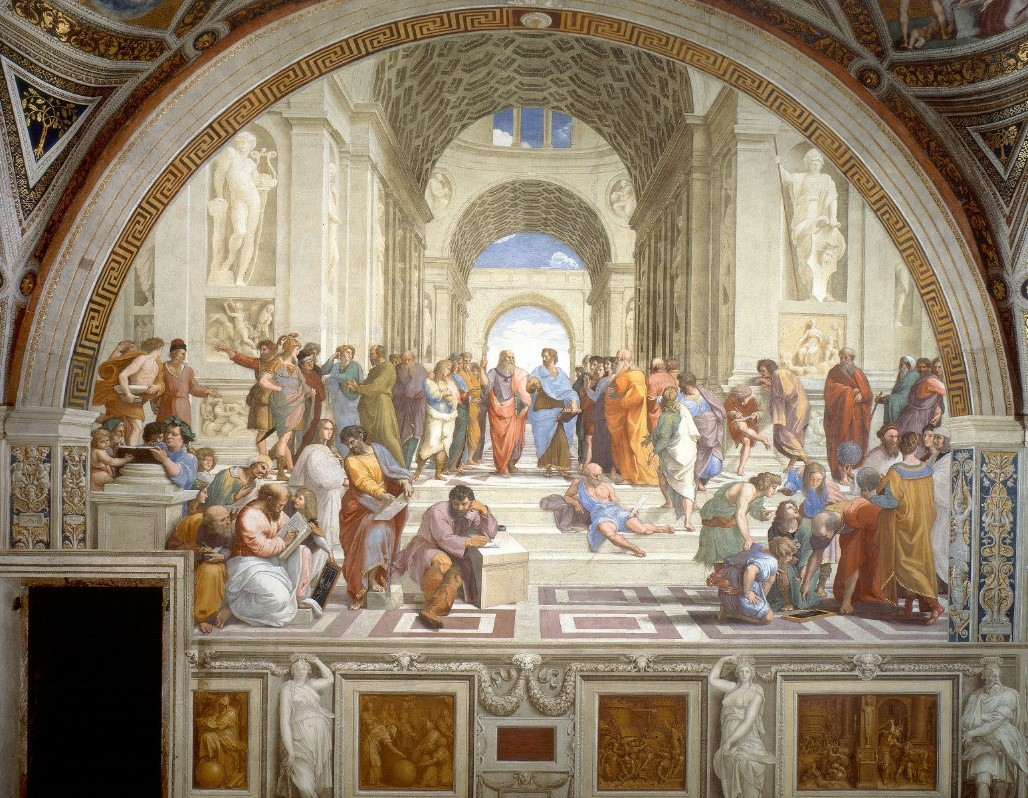
\includegraphics[width=0.9\textwidth]{other/preface_figures/laScuolaDiAtene.jpg}
\captionsetup{type=figure}
\caption{“The school of Athens”, Apostolic Palace, Vatican City. In the centre of the fresco, Plato and Aristotle.}
\end{figure}


\tableofcontents

%\listoffigures


%\listoftables

% \printnomenclature[space] space can be set as 2em between symbol and description
%\printnomenclature[3em]

%\printnomenclature

% ******************************** Main Matter *********************************
\mainmatter

%part 1
\part{DATA-DRIVEN MODELLING}
\chapter{Introduction}

%citazione introduttiva
\epigraph{\textit{How do you know if what you believe is really true?}}{}


This chapter introduces the background of this work identifying its relevance, originality and the placement within the existing literature.\par

The background of this work is engineering. Engineering is composed of models based on math (approximations) that describe a physical phenomenon. The electricity current passing through a wire, the lift force of the air which supports the weight of an aircraft, the exchange of heat in an air conditioning system are physical phenomenon described by engineering models. On-field experiments and observations lead to the definition of the models, i.e. the mathematical relationships between the entities involved in the phenomenon.

\section{Taxonomy} \label{secSupplyChainTaxonomy}

Logistics research is the research domain of this work, which is borderline between engineering and economics. The world \textit{taxonomy} comes from the ancient Greek \textgreek{τάξις} (order) and \textgreek{νόμος} (law). A taxonomy is used to classify the disciplines of a research domain systematically. Figure \ref{fig_operationsResearch} proposes a taxonomy of the logistics research domain. Table \ref{tab_glossaryIntroduction} introduces the glossary with the keywords of this taxonomy.

% INSERT fig_operationsResearch
\begin{figure}[hbt!]
\centering
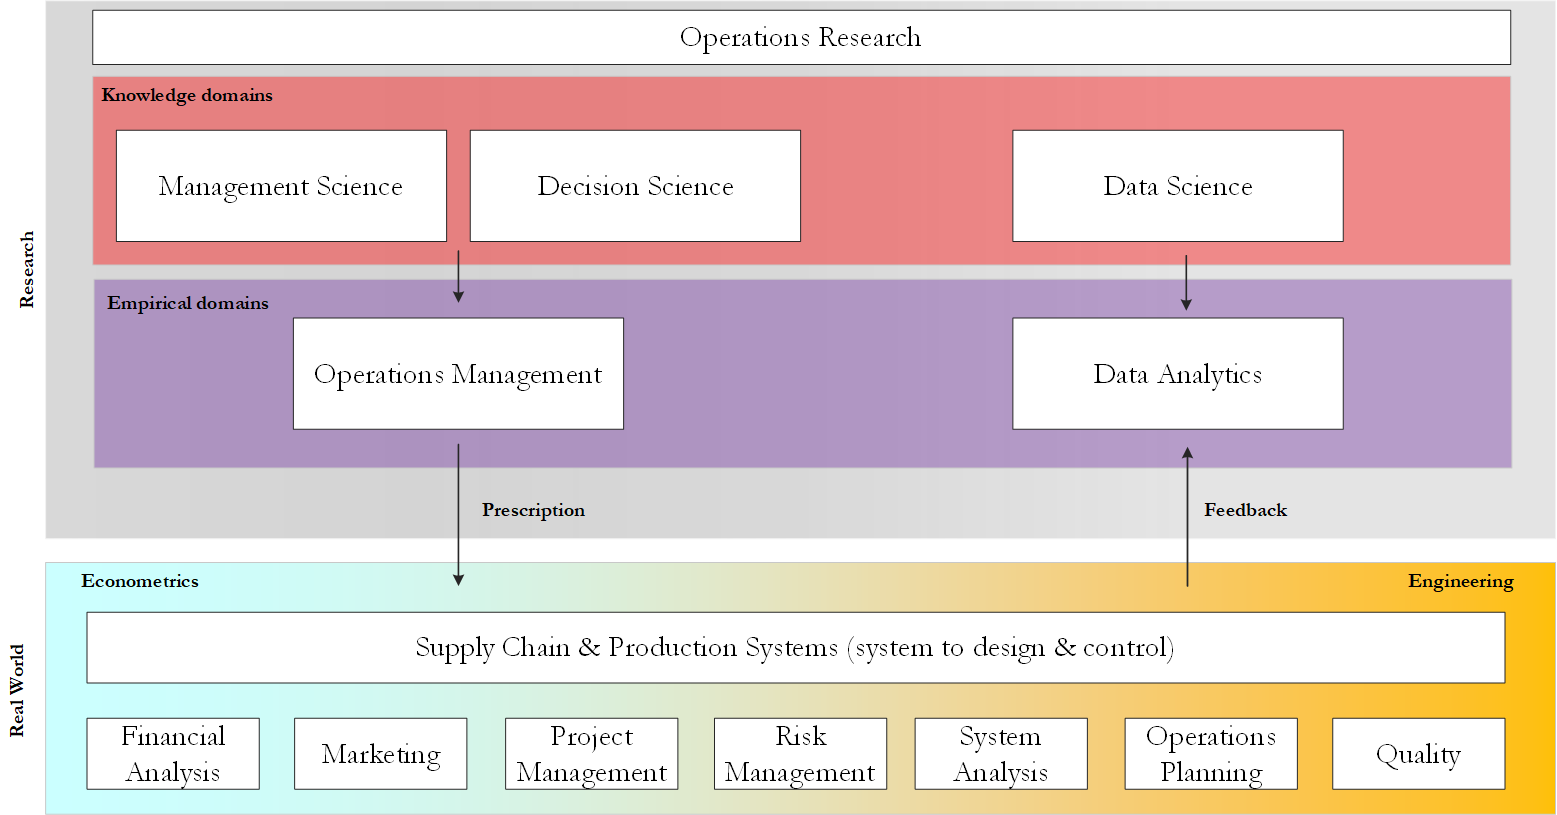
\includegraphics[width=1\textwidth]{SectionIntroduction/introduction_figures/fig_operationsResearch.png}
\captionsetup{type=figure}
\caption{Taxonomy of operations research}
\label{fig_operationsResearch}
\end{figure}


% Please add the following required packages to your document preamble:
% \usepackage{graphicx}
\begin{table}[]
\caption{Glossary of opertions research.}
\label{tab_glossaryIntroduction}
\resizebox{\textwidth}{!}{%
\begin{tabular}{ll}
\hline
Keyword                            & Description                                                                                                                                             \\ \hline
Research domain                    & contributions of academic research on a specific topic.                                                                                                 \\
Real World                         & a physical system.                                                                                                                                      \\
Operations Research                & a research discipline studying the operations (e.g., storage, distribution and production) in the supply chain.                                         \\
Management Science                 & a research discipline studying the relationship between people and resources in an operational context.                                                 \\
Decision Science                   & a research discipline studying the outcome of people’s decisions or expert systems in an operational context.                                           \\
Data Science                       & a research discipline   studying the information content of data.                                                                                       \\
Operations Management              & the outcome of   management and decision science, i.e. a set of models to design and control a   supply chain.                                          \\
Data Analytics                     & a set of models to understand and analyse the information content of a dataset.                                                                         \\
Supply Chain \& Production systems & the set of physical and virtual entities implementing technologies for the realisation, storage and transportation of goods.                            \\
Financial Analysis                 & application of a set of methods to identify the financial position of a physical (e.g., an asset) or virtual (e.g. a stock) entity in the supply chain. \\
Marketing                          & application of a set of methods to connect the demand and offer of a product/service.                                                                   \\
Project Management                 & application of a set of methods to manage resource and time for the realisation of a project.                                                           \\
Risk Management                    & application of a set of methods to manage and control the risk connected to the entities of the supply chain.                                           \\
System Analysis                    & application of a set of methods to manage and control the behaviour of a set of entities in the supply chain.                                           \\
Operations Planning                & application of a set of methods to manage resource and time for the realisation of the product/service.                                                 \\
Quality                            & application of a set of methods   to keep the operations under statistical control.                                                                     \\ \hline
\end{tabular}%
}
\end{table}

This work considers the relationship between decision science and data science proposing a new role of data analytics as a prescriptive tool (together with operations management). The \textit{System Analysis} is the field of application of this work in the supply chain. The following paragraphs introduce the topology for decision \ref{secDecScienceTopology} and data science \ref{secDataScienceTopology}.

\section{Decision Science Topology} \label{secDecScienceTopology}
The word \textit{topology} comes from the ancient Greek \textgreek{τóπος} and \textgreek{λóγοσ}, literally place and study. Differently from taxonomy, the topology studies the “space” of a discipline. In this case, we want to explore which variables influence the nature of the tools used in decision and data science.\par

To define the object of study of this work, we consider the literature ~\cite{Stecca2019} classifying a decision-making process according to:

\begin{itemize}
    \item the number of decision-makers;
    \item their knowledge about the information relevant for a decision. 
\end{itemize}

Usually, a decision-maker (DM) makes a decision (i.e., setting the value of decision variables) based on the knowledge of some information (i.e., decision parameters).\par

A decision process can have single or multiple DMs. We define, accordingly, concentrated and distributed decision making. The information for the decision-making process can be centralised within a single entity/actor or decentralised and owned by several sources. Depending on the topology of information and decision-makers, there are different tools to support the decision process. Figure \ref{fig_decisionsParMak} illustrates this decision topology with classic decision science tools. We analyse four different cases (CC, CD, DC and DD).

% INSERT fig_decisionsParMak
\begin{figure}[hbt!]
\centering
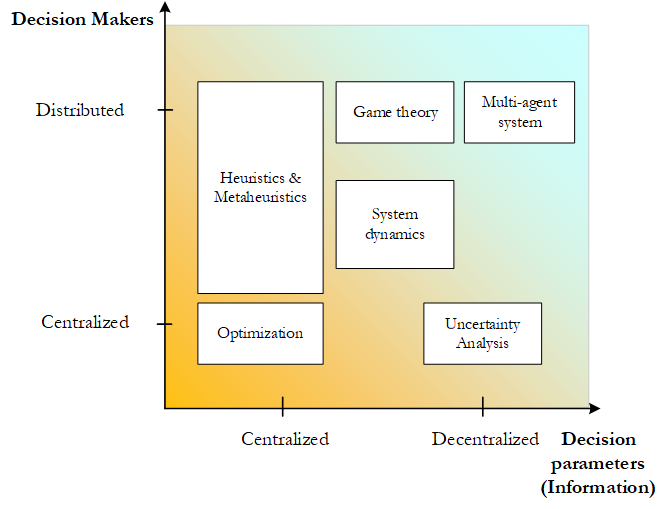
\includegraphics[width=1\textwidth]{SectionIntroduction/introduction_figures/fig_decisionsParMak.png}
\captionsetup{type=figure}
\caption{The Taxonomy of deision support methods.}
\label{fig_decisionsParMak}
\end{figure}

\subsection{Centralised information with centralised decision-makers (CC)}
When a single DM knows all the decision parameters, the optimisation (e.g. integer linear programming, nonlinear programming, robust optimisation) is the most used decision support tool. When the complexity of an instance arises, the optimisation runtime increases exponentially. Under these conditions, suboptimal heuristics or metaheuristics are good alternatives to get proper results within a brief time. A vast number of operational decisions belong to this group since a single person (i.e. the manager) has the responsibility for the decision and the ownership of the information. Some examples are:

\begin{itemize}
    \item the definition of the storage assignment in an industrial storage system;
    \item the job scheduling on a production machine;
    \item the loading sequence of the containers on a vessel;
    \item the definition of the route for a fleet of trucks.

\end{itemize}

An intermediate decision support tool between CC and DC is the “system dynamics”, which defines connection and cause-effect relationships between the decision variables (i.e. the entities of a system) and the DMs. The relationships are usually nonlinear, and the system dynamic evolves at different time steps. The discrete event simulation (DES) is an implementation of system dynamics which evaluates the states of a system at discrete time lags.

\subsection{Centralised information with distributed decision-makers (CD)}
When the output of a single DM depends on the information owned by other DMs, it is necessary to identify different decision scenarios guessing the behaviour of the other actors. Usually, two tools go in this direction:

\begin{itemize}
    \item game theory;
    \item problem-oriented heuristics or metaheuristics algorithms.
\end{itemize}

The game theory assesses the probability of the outcomes of a decision process evaluating all the alternatives in a tree structure. Game theory is mostly used to evaluate the payback of many actors cooperating or not cooperating in a supply chain. All the possibilities of cooperation or not cooperation are evaluated, finding the payback for each actor. Different approaches exist to identify the strategy which provides a higher benefit to a single actor or the entire system.\par

Heuristics and metaheuristics result suitable to provide sub-optimal solutions since they can be tailored to a specific instance of the problem.\par

The definition of the route of a truck is an example of this problem: the planner has all the information, but some decisions (e.g. route replanning) may happen due to exogenous facts as disruptions. 

\subsection{Decentralised information with distributed decision-makers (DD)}

When the information and the ownership of a decision are decentralised, the outcome of the decision process depends on several independent decisions for each actor of the system. An important support tool is the agent-based modelling where each actor (i.e. an agent) has its own set of (partial) information to base its decision. Multi-agent simulation is similar to discrete event simulation. However, each actor implements its specific heuristics to make decisions based on the current state of the system from his point of view (i.e. based on its information set). \par

The participation of a company to a tender is an example of DD; each company makes an offer based on its information. The outcome of the process depends on all the offers from all the companies participating in the tender.

\subsection{Decentralised information with centralised decision-makers (DC)}
When a single DM has the ownership of the decision but not all the information needed, the analysis of the uncertainty is a good choice to deal with the decision process. There are statistical models and methods to evaluate the risk behind a decision (e.g. Montecarlo simulation), and it is possible to infer information finding integrity rules among data. \par

Any CC case with incomplete knowledge on the decision parameters is a DC decision process. The incompleteness can be approached using statistical approaches as Montecarlo simulation or Markov chain to identify confidence intervals on a target variable. It is the case of cost-benefit analysis, where some cost distributions are skewed or hard to estimate.

This book focuses on centralised decision making in the supply chain, i.e. CC and DC cases.


\section{Data Science Topology} \label{secDataScienceTopology}

The previous paragraph introduces a topology of the most used decision support methods without paying attention to the type of data they need. First of all, it is necessary to classify the input data depending on their structure:

\begin{itemize}
    \item structured data. These data usually are from a relational database (e.g., SQL-based) designed using an entity-relationship (ER) model;
    \item Semi-structured data. These data come with a precise but non-relational structure (e.g. CSV, NO-SQL, XML and JSON\footnote{JavaScript Object Notation.} data);
    \item unstructured data. These data have no structure (e.g. text, pictures).
\end{itemize}

In the majority of cases, the literature on logistics and operations works with structured data. Usually, scholars and researchers first approach the methodology to solve a problem and then look for data to validate the approach (model-driven approach). These data are rarely available, and a considerable part of the literature on decision sciences relies on theoretical models validated by randomly generated instances. This research approach supports the development of robust and efficient algorithms, but it does not address real problems. Besides, there is a risk that the problem identified by the researchers does not exist in practice.\par

In this work, we use a different perspective, by introducing the data-driven approach, that is based on the classification in ~\cite{Irv2010} (see Figure \ref{fig_methods}). Data-driven means “let data speak for itself”. The major effort is on understanding the meaning of data and developing a decision support method only after translating data into information.

% INSERT fig_methods
\begin{figure}[hbt!]
\centering
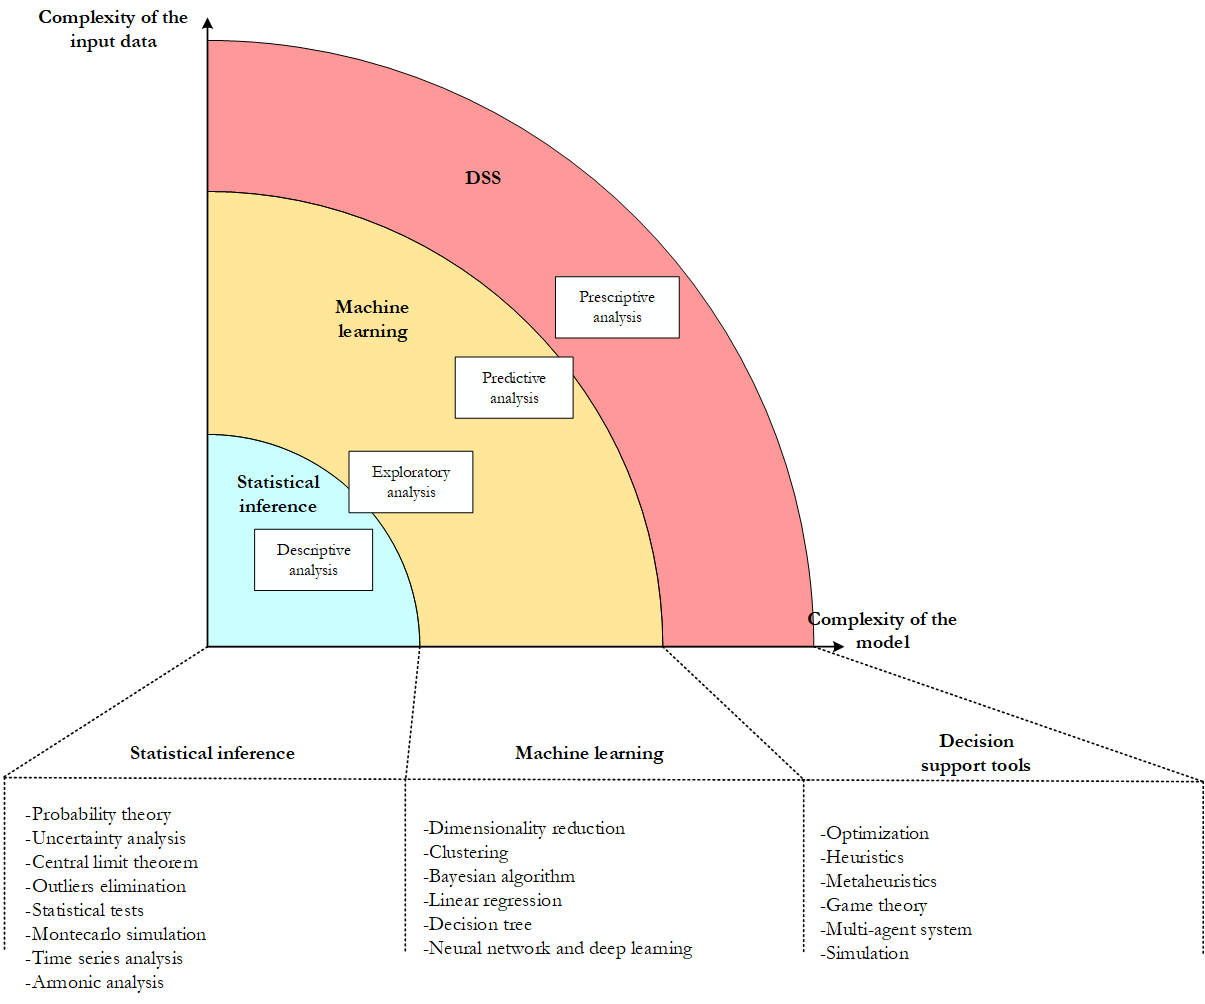
\includegraphics[width=1\textwidth]{SectionIntroduction/introduction_figures/fig_methods.png}
\captionsetup{type=figure}
\caption{The relationship between data and analyticsl methods.}
\label{fig_methods}
\end{figure}

During the last decade, scholars pay attention to data science because of the advent of big data. Big data is the collection, storage and manipulation of data that are \cite{Kitchin2014}:

\begin{itemize}
    \item Huge in storage volume;
    \item High in velocity (e.g., real time);
    \item Diverse in variety (e.g., structured/semi-structured/unstructured);
    \item Exhaustive in scope (i.e., getting the information of a whole population)
    \item Fine-grained in resolution and uniquely indexical;
    \item Relational (i.e., with attributes lining different datasets);
    \item Flexible (i.e., can easily add new attributes);
    \item Scalable (i.e., can easily add new records).

\end{itemize}

Under the perspective of big data, data science opens a new horizon for science. Traditionally, statistical techniques are used to extract knowledge from scarce and static data with weak relations between datasets. This analysis served to answer specific questions (generated under restrictive assumptions) by a researcher with a clear research question in mind ~\cite{Miller2010}. This perspective is changed by big data whose characteristics provides a level of information to explore phenomena without a specific question in mind. Data science introduces a new research paradigm (see Table \ref{tab_paradigms}): Exploratory Science ~\cite{Hey2009}. 


% INSERT tab_paradigms
\begin{figure}[hbt!]
\centering
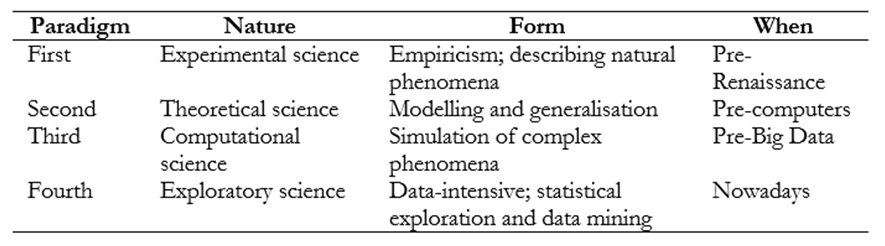
\includegraphics[width=1\textwidth]{SectionIntroduction/introduction_figures/tab_paradigms.png}
\captionsetup{type=table}
\caption{The four research paradigms and their features.}
\label{tab_paradigms}
\end{figure}

The following chapters of this book aim at evaluating when data-driven methods are suitable to address strategic decisions in the field of logistics and operations.

\subsection{Fundamentals of data science}
We start, first, from the fundamental theoretical concepts of data science ~\cite{Provost2013}. 

\begin{enumerate}
    \item Extracting useful knowledge from data to solve business problems can be treated systematically by following a process with reasonably well-defined stages.
    \item Evaluating data-science results requires careful consideration of the context in which they will be used.
    \item The relationship between the business problem and the analytics solution often can be decomposed into tractable subproblems via the framework of analysing expected value.
    \item Information technology can be used to find informative data items from within a large body of data.
    \item Entities that are similar with respect to known features or attributes are similar with respect to unknown features or attributes.
    \item If you look too hard at a set of data, you will find something—but it might not generalise beyond the data you’re observing.
   \item To draw causal conclusions, one must pay very close attention to the presence of confounding factors, possibly unseen ones.

\end{enumerate}

The following paragraphs comes from the (2) and (3) proposing a framework for logistic and operational data. The other points are implemented in the following sections of this work that are dedicated to storage systems, distribution networks and production plants.

\section{History of Operations Research}
Section \ref{secSupplyChainTaxonomy} introduced the research field of this work, while sections \ref{secDecScienceTopology} and \ref{secDataScienceTopology} review the organisation of the decision support tools belonging to the fields of Decision Science and Data Science. The careful readers already will have noticed some overlaps between these two disciplines. Nevertheless, to understand these overlaps and to point out the direction of this work, it is necessary to introduce some history of the operations research (that, in our taxonomy, embeds both Decision and Data Science). \par

Logistics research was born in 1910 with the term “scientific management”, and it is possible to identify eight different periods where technologies, decision making and quantitative methods embed different roles within the same research domain ~\cite{Mortenson2015}:

\begin{enumerate}
    \item Scientific Management (1910-1945)
    \item Scientific Method (1945-1965)
    \item Management Information System (1965-1970)
    \item Decision Support System (1970-1990)
    \item Business Intelligence (1990-2005)
    \item Analytics (2005-2015)
    \item Artificial Intelligence (2015-today)
    \item Non-Human Intelligence (future)

\end{enumerate}

The scientific management of the work (1) starts together with the first assembly line to produce the Ford Model T. For the first time there is a scientific organisation of the work and the time and motion analysis are used to measure and control the productivity of the line. It is the beginning of the application of scientific tools to operations, the era of logistics research began.\par

In the second period (2), after World War II, the Von Neumann's architecture defines how to connect the component of a computer. This architecture changed the world, implementing the separation of the processor and the storage unit of a computer. This architecture is still used today in almost all IT applications, and it opened for the implementation of many decision support tools we still use nowadays.\par

The third period (3) has seen the development of microchips, which make affordable for companies to build information technology (IT) systems. Companies started to collect and store data on their operations into their system.\par

In the fourth period (4), these data are used to improve the decision process through: 

\begin{itemize}
    \item decision support systems (DSS), providing the decision-makers with a suggestion to their problem;
    \item expert system (ES), guiding the DM step by step to get a suggestion to his/her problem.

\end{itemize}

During the period of business intelligence (5), it becomes obvious that there is a value behind the data collected by the IT systems. In addition to companies, the world wide web started providing tons of data and information to a broad public.\par

The period of analytics (6) saw the realisation of the deductive process where information is obtained from tons of data and used to understand and improve the operations. Mathematics is used for understanding the data, but human intuition is still necessary to choose and implement the right decision. According to ~\cite{Mortenson2015}, period (6) was the current one. Nevertheless, the technological developments of the last few years move us to add two additional periods.\par

The period of artificial intelligence (7) starts in 2015 when a team of data scientist from Google develops a neural network able to play the game of Go better than the world champion of this game ~\cite{Silver2016}. It is the advent of artificial intelligence. IT systems have already overcome the speed of the human brain (during period (6)), but now they are also able to think and react similarly to a real human brain. The following step is theoretical, but natural (8): when the artificial systems will be able to program themselves, they will be able to understand a problem autonomously and to get a solution faster and better than a real human brain. However, for the sake of our knowledge, this step in the history of IT is yet to come.\par

This work focuses on step (6) in the field of logistics and operations. We want to approach analytics to deeper investigate how human intuition and the value of logistics information match for proper management of a supply chain ~\cite{Arvan2019}.\par

Accordingly to the periods defined above, step (6) should already be out-to-date. Nevertheless, the literature (see chapter 2) shows that few papers study analytics from a research point of view and their application in the logistics practice is still rare. The majority of supply chain systems stopped at the stage (4) where complex ES and DSS are seen as the final weapon against the inefficiencies of the supply chain.\par

Big companies use analytics to profile customers, price products and make financial analysis (the green shade in Figure 1). Nevertheless, they rarely studied analytics for engineering applications whose potential is even higher due to big data available from production, tracking and other activities in a supply chain. 

\section{A change in the perspective}

Figure \ref{fig_operationsResearch} illustrates the topology of logistics research and the traditional role of decision science and data science. Here we want to investigate their role from a control perspective. Traditionally, decision science is used to model the system to control (e.g. a supply chain or a plant), and data science is used to get relevant data and keep the variables of the system under control. Figure \ref{fig_controlDataDriven} illustrates the differences between a data-driven and a model-driven approach ~\cite{Hedgebeth2007}, which will now be investigated, from a system control perspective. It is important to remark that a model is never the reality, but a useful approximation used to get information on it ~\cite{Hazen2014}.

% INSERT fig_controlDataDriven
\begin{figure}[hbt!]
\centering
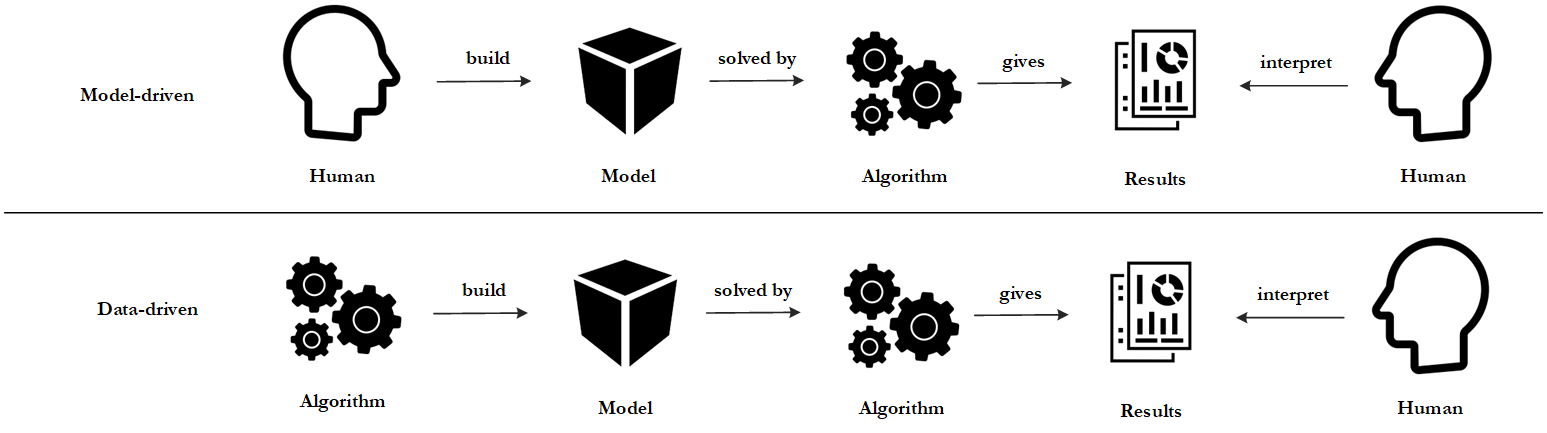
\includegraphics[width=1\textwidth]{SectionIntroduction/introduction_figures/fig_controlDataDriven.png}
\captionsetup{type=figure}
\caption{Model-driven vs. data-driven learning process.}
\label{fig_controlDataDriven}
\end{figure}

The traditional model-driven approach can be seen as a system to control through a feedback loop:

\begin{enumerate}
    \item the real system is modelled through decision science, defining decision variables based on the human understanding of the system;
    \item the historical data of the system is the input parameter of the model;
    \item the output of the model is analysed and used again to control the system.

\end{enumerate}

Here we have a traditional model-driven approach (see Figure \ref{fig_controlAsIs}) where the “system model” is an ES or a DSS.

% INSERT fig_controlAsIs
\begin{figure}[hbt!]
\centering
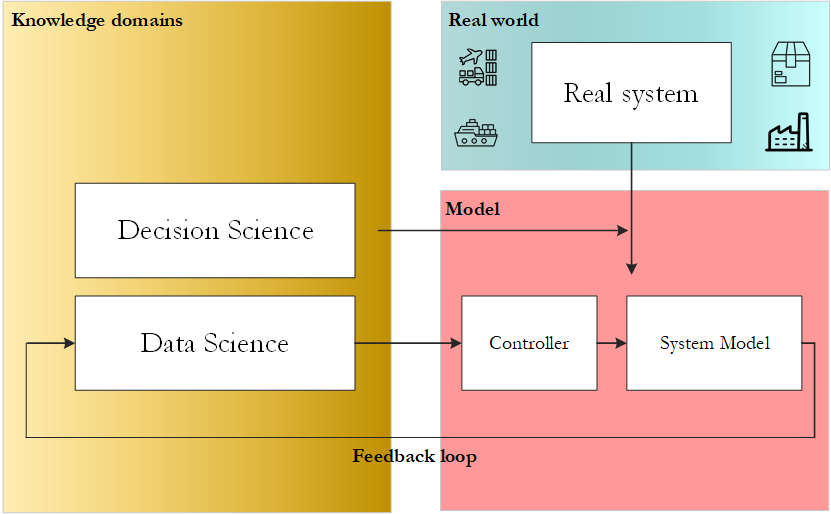
\includegraphics[width=1\textwidth]{SectionIntroduction/introduction_figures/fig_controlAsIs.png}
\captionsetup{type=figure}
\caption{Traditional model-driven approach, based on feedback control.}
\label{fig_controlAsIs}
\end{figure}

In this work, we introduce a different approach (see Figure \ref{fig_controlToBe}). Data science is not only the base for the control of the system but also the design of the model. Figure \ref{fig_controlDataDriven} already illustrated the differences between model-driven to data-driven perspectives.

% INSERT fig_controlToBe
\begin{figure}[hbt!]
\centering
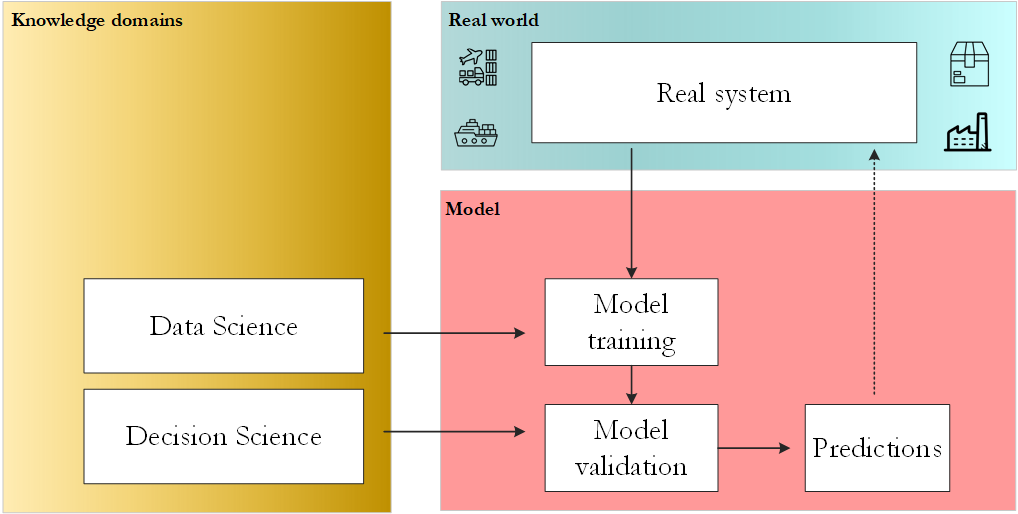
\includegraphics[width=1\textwidth]{SectionIntroduction/introduction_figures/fig_controlToBe.png}
\captionsetup{type=figure}
\caption{Novel data-driven approach, based on predictions.}
\label{fig_controlToBe}
\end{figure}

By using this approach, data science is used to train a model which is based on the real behaviour of the system and not on apriori human intuition. The outcome of the model which highlight patterns, correlations and relationships among data are discussed and interpreted by human and used as input for decision-making. The model is, then, used to predict the behaviour of the system in the future. The model is trained and updated each time new historical data from the real system are available, making the data-driven approach flexible and up-to-date. We can think of this fact as the change from a world where there was the need to design from scratch to a world where it is necessary to understand, control and improve the extant processes. This is the reason why the following sections of this book analyse the control of a logistic system first.\par

This approach does not question the relevance of decision science, but it considers a new relationship between data science and decision science. We can exemplify this new relationship thinking of the design of a DSS. We identify the four fundamental stages in the design of a DSS from a data-driven perspective (whose implementation will be the object of Parts III, IV and V of this book):

\begin{enumerate}
    \item diagnosis of the real system (business-as-usual);
    \item training of the model;
    \item validation of the model;
    \item deployment of the DSS.

\end{enumerate}

The diagnosing of the business-as-usual scenario (1) is the phase where the DM assesses the problem, its environment, its criticalities, identify the managerial question to answer and the KPIs to measure the goodness of possible answers. In this phase, the DM takes a “snapshot” of the real system using statistical inference and data visualisation to:

\begin{itemize}
    \item understand the business-as-usual process;
    \item identify the level of information at his/her disposal.

\end{itemize}

The training of the model (2) is the phase where the decision variables are identified and the model to predict their value is built (based on data science methods). The model is trained upon the available data from the real world. Differently from the model-driven approach, we do not assume any relationship between the input variables. In some case, assumptions are made on the value of each column to clean the data but, in general, we are interested in augmenting the knowledge we have on the data by only observing the data. For this reason, other assumptions are discouraged at this stage. The model will highlight the relationships between the input data and the decision variables.\par

Human intuition is then required to understand the output of the model and the link between the input data that is the validation of the model (3). Decision science methods can be implemented at this stage when the scenario is complex, and it requires additional information to be useful for the DM (e.g. it is necessary to merge the results of two models trained on different decision variables).\par

When the output of the model is considered confident enough for the DM (and from a statistical point of view), the model can be deployed into a DSS (e.g., a software) able to get input, train the model and present the output aiding the DM in his/her work.\par

This work proposes a novel approach where data-driven models are used together with the traditional scholars’ model-driven approach. In other words, instead of modelling a logistic/operations process based on human understanding, the modelling phase is based on the data available from the measurement of that process.\par

A human effort is required in the organisation of the measurement data and the understanding of the outcome of the model. In other words, we switch from the control of a logistic/operation process to the prediction of the outcome of that process. In this work, we use the terms “data-driven”, “logistics 4.0”, “smart logistics”, supply-chain 4.0” and “predictive logistics” to indicate this change of perspective.

\section{Towards Predictive-Prescriptive Optimisation}
Model-driven and data-driven models can co-exist. For this reason, we introduce the mathematical formulation of a problem addressed together by them ~\cite{Bertsimas2014}). We introduce here the general formulation of:

\begin{itemize}
    \item data-driven optimisation;
    \item supervised learning;
    \item predictive-prescriptive problem.

\end{itemize}

Let introduce the following variables. Let $y_1,\ldots,y_N\in Y$ a quantity of logistics/operational interest (e.g. the demand); $x_1,\ldots,x_N\in X$ be an associated covariates $X$ (e.g. search engine attention); $z\in Z$ the decision variables.

In data-driven optimisation, we are interested in setting decision variables $z$ to minimise an uncertain cost $c(z;Y)$. We only consider the prescriptive approach (i.e. defining the values of $z$) and the historical data $Y$. The problem can be written as:

\begin{equation}
    min_{z \in Z} \left[ c(z,Y) \right]
\end{equation}

The solution to the problem can be found by sample average approximation solving the problem with different replication of the input variable $Y$:

\begin{equation}
    {\hat{z}}_N^{SAA}\in\arg{\min_{z\in Z}{\frac{1}{N}\sum_{i=1}^{N}{c(z;y^i)}}}
\end{equation}

The “pure” supervised learning approach, on the other side, does not involve prescription but focuses on the prediction (i.e. the forecast) of the future values of $Y$ given the historical values of $Y$ and $X$. In other words, we are looking for a prediction ${\hat{m}}_N(x)$ for the future value of $Y$ after observing $X=x$ and $Y=y$. The problem can be written as:

\begin{equation}
    E \left[ Y|X=x \right]
\end{equation}

The problems defined by (1) and (3) matches together in the predictive-prescriptive problem i.e. fitting a machine learning (supervised) model ${\hat{m}}_N\approx\ E[Y|X=x]$ and then solving a deterministic problem:

\begin{equation}
    {\hat{z}}_N^{point-pred}\left(x\right)\in\arg{\min_{z\in Z}{c(z;{\hat{m}}_N(x))}}
\end{equation}

An optimal solution to the problem can be found as:

\begin{equation}
    z^\ast(x)\in arg min_{z\in Z} E[c(z;Y)|X=x]
\end{equation}

Roughly speaking,  predictive-prescriptive optimisation works:

\begin{enumerate}
    \item finding a relationship (i.e. a predictive model) between  the set of variables $X$ and $Y$;
	\item exploring the cost $c$ of different configurations of $Y$, predicted by different settings of $X$;
	\item Averaging over different replicates finding the set of decision variables $z$ connected to the minimum of $c$.

\end{enumerate}

\section{The quality of data}

Data-driven methods offer the technology to substitute some knowledge-based roles of a human by a machine. Nevertheless, we would like to know how much accurate can a machine be. In other words, if a company needs a logistic expert, they hire (or train) a person with a logistic background. How can we measure the degree of competence of a machine?\par

The outcomes of a data-driven process always depend on the quality of the input data ~\cite{Hazen2014}. We can think of the data production process as a manufacturing process with three stages:

\begin{enumerate}
    \item raw data;
    \item data processing;
    \item data product.

\end{enumerate}

The \textit{data product} is the final product of a data collection process and, as for physical products, it is possible to measure its quality. The higher the quality of the data product, the more robust the results of a data-driven model fed by the data product. We identify four metrics to measure the quality of a data product (see Table \ref{tab_dataQuality}).

% INSERT tab_dataQuality
\begin{figure}[hbt!]
\centering
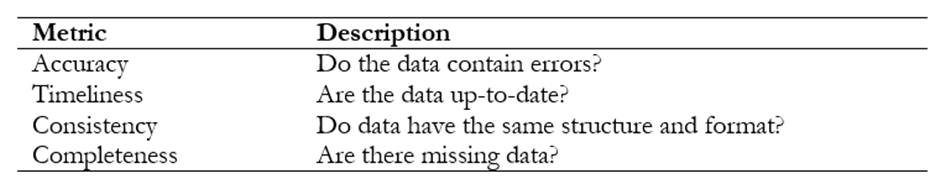
\includegraphics[width=1\textwidth]{SectionIntroduction/introduction_figures/tab_dataQuality.png}
\captionsetup{type=table}
\caption{Metrics to measure the quality of data.}
\label{tab_dataQuality}
\end{figure}

The accuracy identifies if data corresponds to the real values. Timeliness describes if data records are up-to-date (currency) and their update frequency (volatility). Consistency regards the robustness of data format and data structure. Completeness measures the fraction of missing data over the total information content. It is important to check the quality of the input data before starting with data-driven modelling since poor data quality is the most common cause of bad predictions.


%\clearpage
\bibliographystyle{ieeetr}
\bibliography{SectionIntroduction/introduction_ref}




\chapter{Research Background}

%citazione introduttiva
\epigraph{\textit{The line between statistics, computer science and engineering is getting thinner.}}{}


This chapter reviews the relevant literature identifying the academic position of this work. As introduced, this work provides advances in the field of engineering applied to the “system analysis” (see Figure \ref{fig_operationsResearch}) of a supply chain by using data-driven technologies.\par

Before starting with this data-driven journey, it is necessary to introduce a brief glossary with the keywords used to gather academic papers by scholars and practitioners (see Table \ref{tab_dataGlossary}).

% INSERT tab_dataGlossary
\begin{figure}[hbt!]
\centering
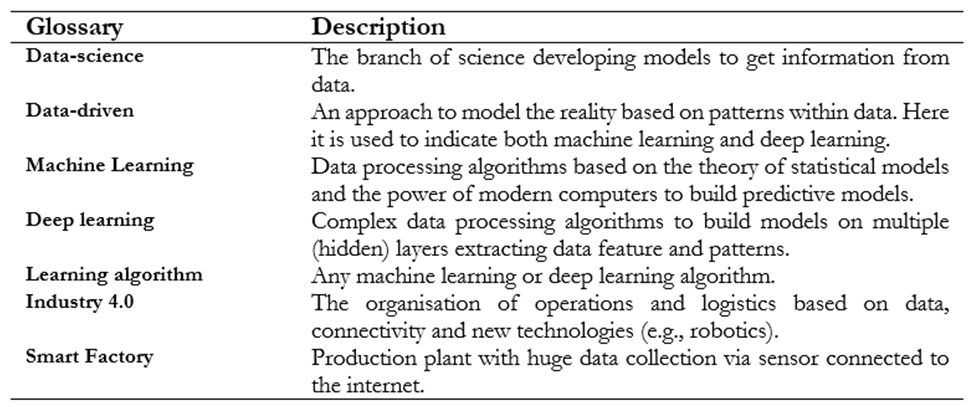
\includegraphics[width=0.9\textwidth]{SectionIntroduction/researchBackground_figures/tab_dataGlossary.png}
\captionsetup{type=figure}
\caption{Glossary of data science terms.}
\label{tab_dataGlossary}
\end{figure}

\section{Academic background}

The data-driven approach is gathering an increasing interest in literature during the last decade. In particular, the number of research paper approaching logistics research issues from a data-driven perspective is increasing exponentially ~\cite{Moktadir2019, Spanaki2018}. Figure \ref{fig_literature_trend} illustrates research trends on Scopus reporting the number of research papers published in international journals resulting from four research queries. The world “machine learning”, “deep learning” and “data-driven” are used together with the word “industry” to check how literature evolves approaching this topic from an industrial perspective. The last trend is focused on the field of supply chain management. This trend is similar, but with a lower absolute number of papers.

% INSERT fig_literature_trend
\begin{figure}[hbt!]
\centering
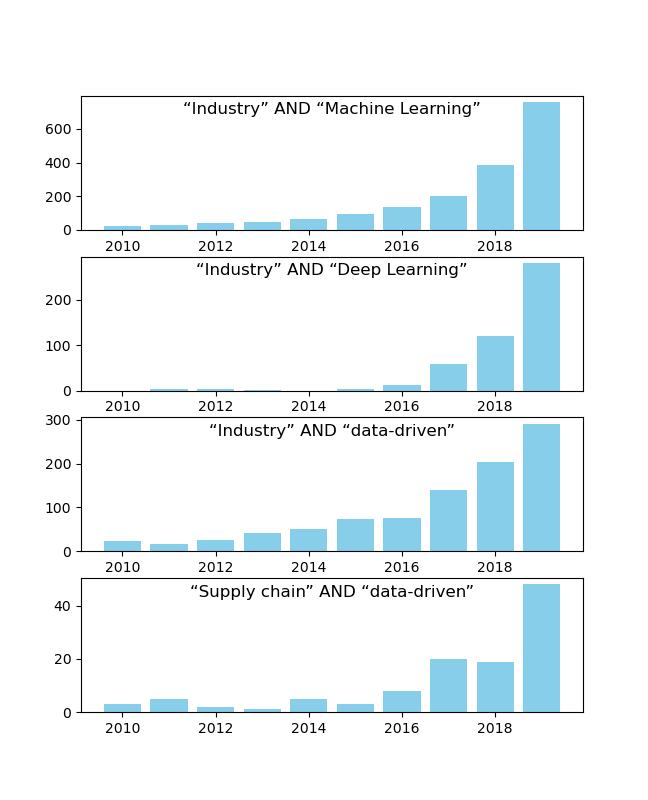
\includegraphics[width=0.9\textwidth]{SectionIntroduction/researchBackground_figures/fig_literature_trend.png}
\captionsetup{type=figure}
\caption{Literature trends corrsemponding to different research queries on Scopus.}
\label{fig_literature_trend}
\end{figure}

This analysis shows that, in the last few years, scholars are paying more attention to data-driven approaches applied to industrial fields. Nevertheless, the amount of contributions in the field of industrial engineering and supply chain is still limited. A closer investigation of the industrial engineering field confirms the need for a broader study of data-driven methods in this field ~\cite{Nguyen2018}. Figure \ref{fig_literature_pie} categorises the topic of industrial engineering approached with a data-driven approach in a sample of 23 journal articles.

% INSERT fig_literature_pie
\begin{figure}[hbt!]
\centering
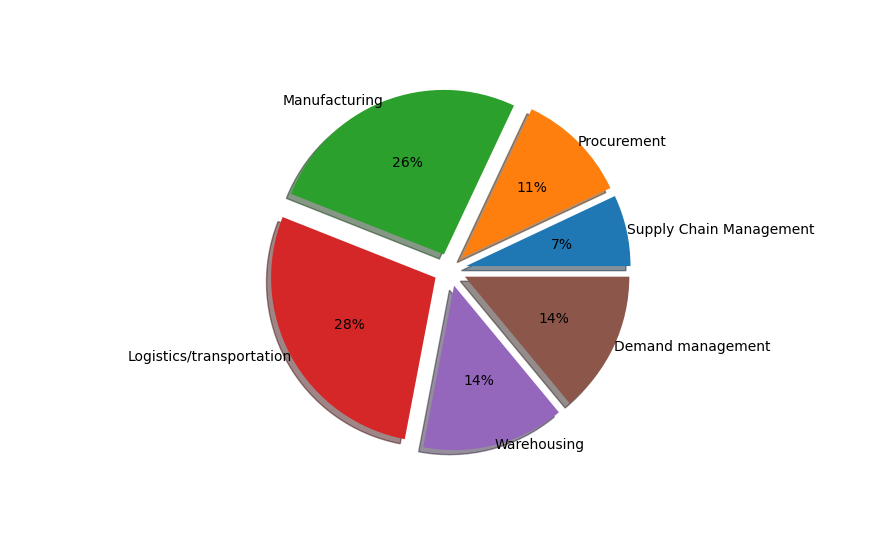
\includegraphics[width=0.9\textwidth]{SectionIntroduction/researchBackground_figures/fig_literature_pie.png}
\captionsetup{type=figure}
\caption{Fields of application of data-driven algorithms in the industrial engineering sector.}
\label{fig_literature_pie}
\end{figure}

Industrial engineering shares engineering and decision science features. Figure \ref{fig_topics_pie} (defined on a sample of 52 journal articles) shows that both of them are areas of research where analytics and data-driven modelling are established methodologies ~\cite{Gupta2019}.

% INSERT fig_topics_pie
\begin{figure}[hbt!]
\centering
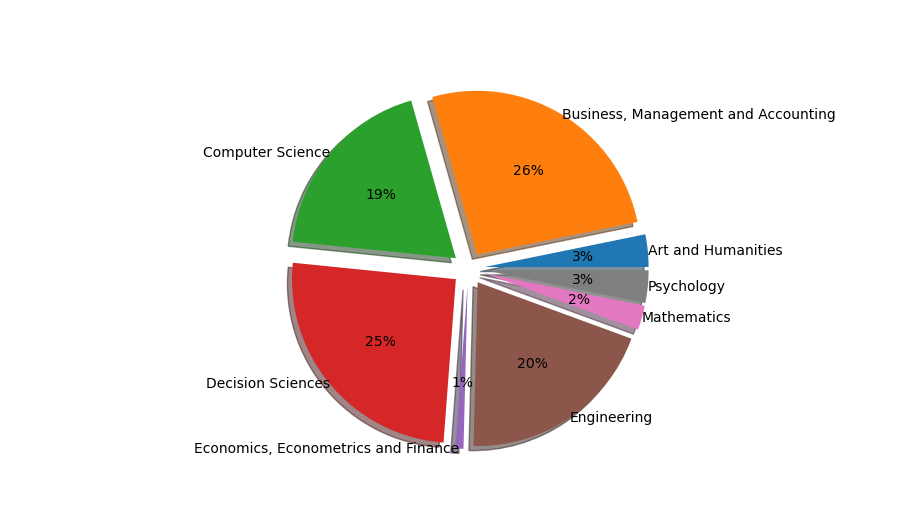
\includegraphics[width=0.9\textwidth]{SectionIntroduction/researchBackground_figures/fig_topics_pie.png}
\captionsetup{type=figure}
\caption{The fields of application of data-driven algorithms.}
\label{fig_topics_pie}
\end{figure}

The literature lacks a comprehensive approach of data-driven models in the field of logistics research as tools for system analysis ~\cite{Wang2016, Lamba2018}. Many papers show frameworks for the application of analytics and data-driven methods to sub-topics as safety engineering, industrial database design data structures and real-time data collection with internet-of-things (IoT) industrial devices ~\cite{Huang2018, Zhang2018}. Nevertheless, none of them proposes a holistic point of view on logistics and operations.\par

On the other side, they clearly recognise a value behind data ~\cite{Balandin2015, Uckelmann2008} and the importance of smart logistics and smart factory whose capability is to adapt decision making dynamically to predict future scenarios.\par

This new approach involves a large mass of data exchanged between several actors ~\cite{Kawa2012, Singh2017}. Literature suggests robust methodologies to manage the information flow of data ~\cite{Tran-Dang2018}. The outcome of these data structures supports the development of the smart factory, i.e. a manufacturing plants where information is used to control the process and to make decisions on the future processes (i.e. the design) ~\cite{Hajdul2011}. \par

In ~\cite{TAN2018}, they identify three main research issues to improve the operation in a smart factory using data-driven methods:

\begin{enumerate}
    \item modelling the theory and method of smart factory;
    \item knowledge discovery and knowledge management based on industrial big data analysis;
    \item adaptive scheduling and optimisation of the smart factory.

\end{enumerate}

This book focuses on the key issues (2) and (3). Often, literature focuses only on theoretical frameworks for the application of data-driven methods ~\cite{DaSilva2019}. In this work, we aim at a comprehensive approach for logistics and operations being practice-ready for a company proposing areas of application of data-driven methods.

\section{Industrial background}
In addition to the academic relevance, we want to highlight the rationale of this work considering the structure of the external industrial sector: data science is the present, not the future. In the last decade, companies started creating a new professional role called “data scientist” able to generate value from industrial data. From this perspective, the statistic is the history, machine learning is the past, and deep learning is the present ~\cite{HubSpot2016}. These methodologies have already been established and implemented in many business areas (e.g. marketing, finance) with or without the contribution of the research community since a number of companies recognised their data could be used to improve the efficiency, reliability and sustainability of their business ~\cite{Nascimento2019, Trkman2010}.\par

Looking at the industrial practice, we notice that there is an enormous potential for data-driven application in the field of logistics. The industry is reacting to this new trend with significant investments in data-driven projects ~\cite{Worldeconomicforum2017, Zhong2016}. Managers and directors from logistics and operations identify in the big data analytics the main tool to handle decision and processes in the future ~\cite{Rossmann2018}. Nevertheless, a significant gap exists between large companies, able to train data scientist themselves, and small and medium enterprises (SME) which cannot afford this kind of investment ~\cite{Dubey2019}.\par

It is the case of large third-party providers that develop machine learning and artificial intelligence tools to support their business ~\cite{Ku2018}. They identify a precise workflow to check if a data-driven approach can be used to generate value, improving a logistic process (see Figure \ref{fig_applicationML}) with two main activities:

\begin{enumerate}
    \item creating new knowledge;
    \item reducing costs.

\end{enumerate}

% INSERT fig_applicationML
\begin{figure}[hbt!]
\centering
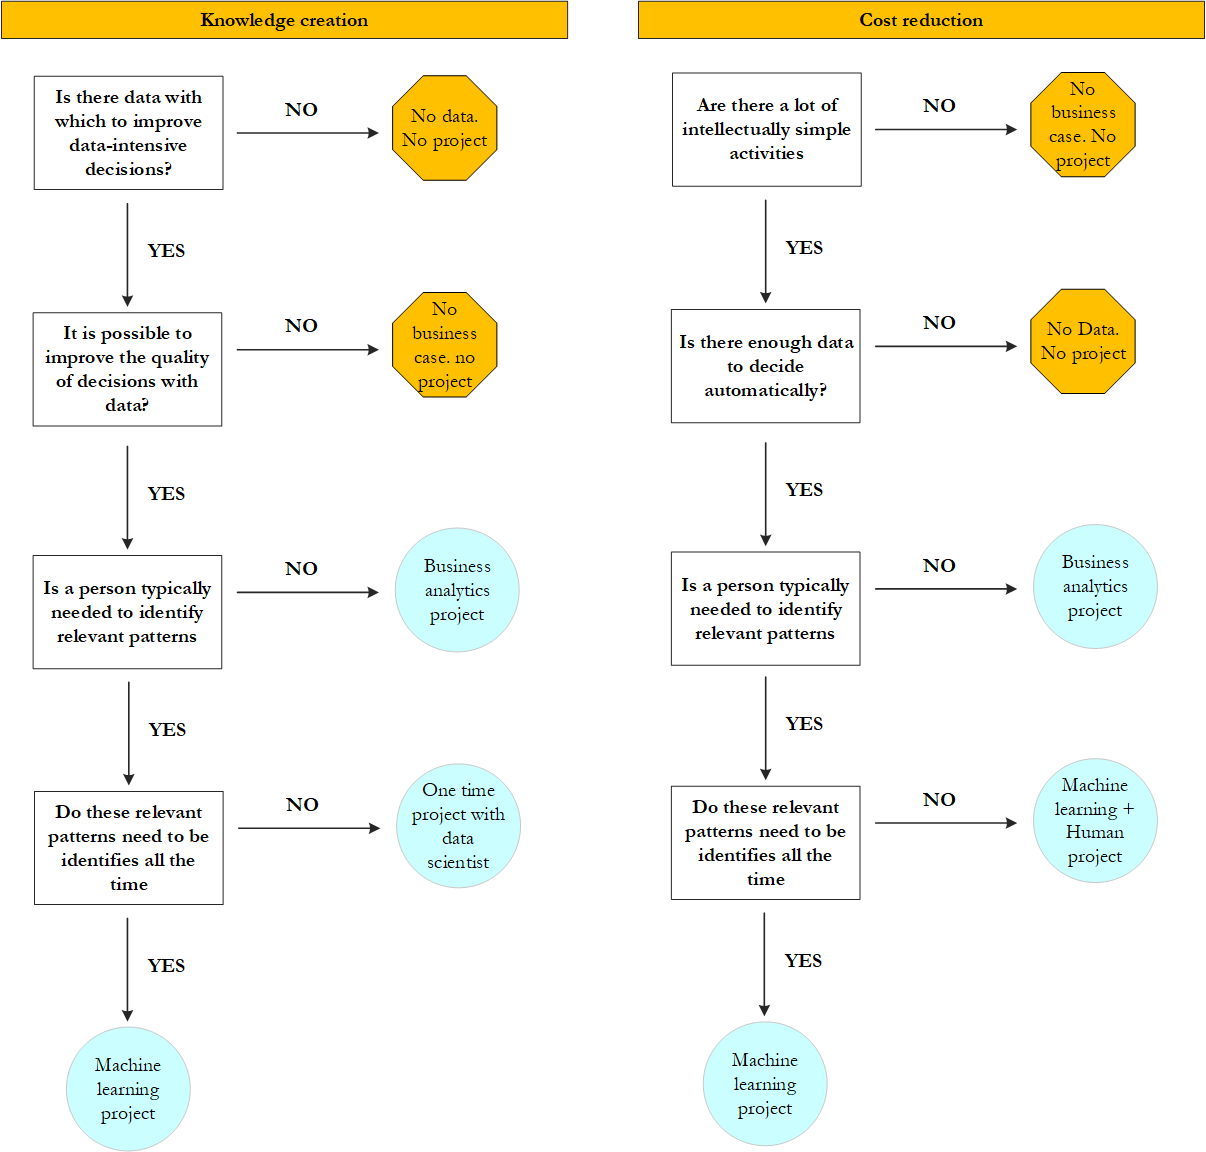
\includegraphics[width=0.9\textwidth]{SectionIntroduction/researchBackground_figures/fig_applicationML.png}
\captionsetup{type=figure}
\caption{Checklist for the implementation of a data-driven project adapted from ~\cite{Ku2018}.}
\label{fig_applicationML}
\end{figure}

These two objectives are the reason why companies started collecting data on their processes and hiring data scientists. The flowcharts in Figure \ref{fig_applicationML} identify the necessary ingredients to get success from data-driven approach. The quantity and quality of the data is, obviously, a crucial issue to work with a data-driven approach. Besides, the data collected must be relevant to solve a decision problem. Finally, if an algorithm can find patterns better than a human does, the data-driven approach is a good choice to create knowledge and reduce costs.\par

Both these objectives are reachable when data scientists have both analytic skills and profound knowledge of the industry-specific domain ~\cite{Ku2018}. When these two characteristics come together, data-driven application leads these companies to success while some small logistics companies still strive to work with pen and paper.

Logistics companies identify the need to anticipate the behaviour of the market with predictions on:

\begin{itemize}
    \item lead times;
    \item transport capacity;
    \item customer orders. 

\end{itemize}

Predictive logistics can forecast the value of these metrics anticipating market demand. Traditional logistics is way less efficient and unable to anticipate market behaviour ~\cite{LOGISTICAEFFICIENTE2019}. Data-driven tools are not limited to transportation activities.  Recent applicationS in the manufacturing and storage industry have seen several predictive models to support the operations ~\cite{Logisticofthings2017, Package.ai2017, Reporter2016}.\par

While a small number of big companies recognises the value of its operational data, researchers strive to get data to test their assumptions enriching the literature and public knowledge. Besides, the more these companies see a profit in their data-driven approaches, the less they are willing to share data with the research community. This happens because they get a competitive advantage from the utilisation of their data and sharing their valuable knowledge with the public would not be safe for their business.\par

In this sense, our work is even harder since it is difficult not only to design new methods but also to get data to test them and keep them useful in the real world. For this reason, we notice a gap between practice and academic research, especially when internal research units of multinational companies hold the data and autonomously lead the research activities.\par

Also, the application of data-driven models in industrial practice is still limited in the field of logistics and operations ~\cite{Garver2019}. We think that academic research has the responsibility to explore the role and the potential of analytics and data-driven methods in the logistics and operations fields.\par

%\clearpage
\bibliographystyle{ieeetr}
\bibliography{SectionIntroduction/researchBackground_ref}

\chapter{The Information Framework} \label{chap_InformationFramework}

%citazione introduttiva
\epigraph{\textit{Pure mathematics is, in its way, the poetry of logical ideas.}}{Albert Einstein}


Supply chains involve a large number of connected entities, resources, actors and flows.  In this chapter, we introduce a framework to model the entities of storage systems, distribution network and production plants. In particular, this work investigates the room for the application of data science in the field of logistics and operations. For this reason, we are interested in mapping the information relationships between these entities.\par

Here we introduce an ontology of entities and metrics. This ontology meets the \textit{fractal manufacturing system} philosophy (see \cite{Sprock2018}), where each element of a supply chain can be seen as a black box with input and outputs. The elements can be aggregated or disaggregated into other black boxes. In the following parts of this book, we will re-define this ontology by applying it to smaller blocks of the supply chain, with specific references to storage systems, distribution networks and production plants.

\section{Ontology}\label{secOntology}
We base our ontology on \cite{Hopp2011}, a milestone book in logistics and operations science. It was the first providing a scientific framework to model a factory. 

\subsubsection{Entities}
We identify the following entities.\par
\textbf{Part} ($i$): it is a piece of raw material, component, subassembly or assembly. Where:
\begin{itemize}
    \item Raw material is a part purchased out of the system.
    \item Component is an individual piece assembled into more complex products.
    \item Subassembly is an assembled unit further assembled into more complex products.
    \item Assembly/final assembly/finished product is the fully assembled product.
\end{itemize}
\par
\textbf{Processing node} ($j$): we define the processing node using the concept of fractal manufacturing. From this perspective, a processing node is any entity that can be modelled as a black box with input and output. A production machine, a production line, a packing machine, a manufacturing robot, a production plant, a storage system, a port, a logistic platform, a train terminal are all examples of entities working as a processing node. A processing node usually performs value-added activities on a part. \par

\textbf{Edge} ($j,k$): it is a physical connection between processing nodes. Aisles and conveyors are edges in a production plant while railways, rivers and roads are the edges of a distribution system.\par

\textbf{Vehicle} ($v$): a vehicle is a handling unit able to transport one or more parts from a processing node to another. Operators, forklifts, AGVs, trucks, trains, vessels are all examples of a vehicle. \par

\textbf{Consumable} ($s$): a consumable is a material that is used by a processing node or a vehicle to perform its work. A consumable is generally responsible for the variable costs of the processing node or a vehicle (e.g. energy and fuel).\par

\textbf{Route} ($e$): is the sequence (ordered set) of processing nodes $j=1,\ldots,m$ visited by a vehicle to add value on a part.\par

\textbf{Order} ($o$): is a processing request on a part sent by a customer. \par

\textbf{Job} ($b$): is the response to the market demand from the operations side. Production batches and transportation loads are examples of a job.\par

\textbf{System network} $G(V,A)$: the system network is the set of processing nodes $j\in V$ and edges $\left(j,k\right)\in A$ that connect all the entities involved in the supply chain system.

\subsubsection{Metrics}
We identify the following metrics to assess the performances of a processing node $j$.\par

\textbf{Throughput} ($TH_{j}$): the throughput of a processing node is the average output per unit of time (e.g., parts per hour).\par

\textbf{Work in process} ($WIP_{j}$): is the number of parts (i.e., the level of inventory) being processed/waiting for processing by a processing node.\par

\textbf{Work in process} ($WIP_{jk}$): is the number of parts (i.e. the inventory position) being transported on edge $(j,k)$ by a vehicle $v$. \par

\textbf{Capacity} ($C_j$): is the upper bound of the throughput.\par

\textbf{Capacity} ($C_v$): is the maximum capacity of a vehicle $v$. \par

\textbf{Utilisation} ($U_j$): it is the fraction of time that a processing node is not idle for lack of demand. \par

\textbf{Utilisation} ($U_v$): is the fraction of transportation space that a vehicle uses due to the variability of the transportation demand. \par

\textbf{Lead time} ($LT_e$): is the time allocated for a given route. \par

\textbf{Cycle time} ($CT_e$): is the average time from the release of a job to the end of its route. \par

\textbf{Service level} ($SL_e$): $Prob\{cycle\ time\le lead\ time\}$

Little’s law (see equation (\ref{eq_littlesLaw})) defines a basic relationship linking the three main metrics, i.e. $WIP$, $TH$ and $CT$.

\begin{equation}
WIP_j [pz]=TH_j \left[\frac{pz}{h}\right] \times CT_{e:e \in \{j\} } [h]
\label{eq_littlesLaw}
\end{equation}

Usually, managers have data on the entities at their disposal, but they need to get information on the metrics. This data can be dirty or incomplete. For this reason, we build upon this ontology to show how to infer the properties of entities and metrics when data are incomplete or missing.\par

Our approach is highly generalisable and based on a few standard rules of a supply chain, with minimum bias. For this reason, the theoretical effort of this work stands in the definition of a structure for industrial data and the understanding the role of data features and the consistency rules among different features that can be used to increase the value of an incomplete dataset.\par

The modelling of a system accordingly with a robust data structure allows using only logistics-relevant data and base the model on robust relationships. The following sections define this data structure for storage, distribution and production systems. We first introduce the law of physics to analyse the material flows of a supply chain. Then, a theorem regulating the consistency of the information flow is introduced and demonstrated.\par


\section{The physics of a supply chain} \label{sect_supplyChainPhysics}

The laws of physics can be used to model the material flows between the entities of a supply chain. We can think of a processing node $j$ as a physical system with an inventory $WIP_j$ subjected to “forces” modifying its value. It is not difficult to imagine that the value of $WIP_j$ can change when:
\begin{itemize}
    \item some forces \textit{pull} a number of items from $j$;
    \item 	some forces \textit{push} a number of items into $j$.
\end{itemize}

% INSERT fig_processingNode
\begin{figure}[hbt!]
\centering
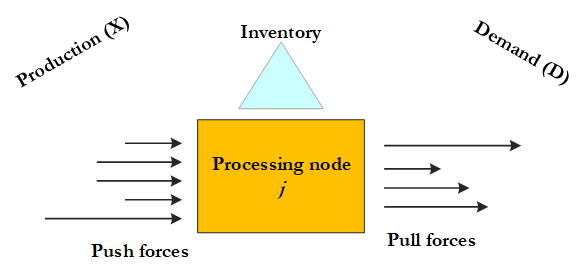
\includegraphics[width=1\textwidth]{SectionIntroduction/informationFramework_figures/fig_processingNode.png}
\captionsetup{type=figure}
\caption{Physical model of a processing node.}
\label{fig_processingNode}
\end{figure}

Figure \ref{fig_processingNode} presents a scheme of the physical model of a processing node where the forces generated by the production and the demand modify the value of the inventory.\par

The concept of a \textit{force} modifying the inventory matches very well with the definition of pull and push production philosophy. The analysis of push and pull systems is out of the scope of this book. We will limit to describe the dynamics and the rules of these systems using the idea of a \textit{force} associated with the production and the demand. To model $j$, we are just interested in defining how these forces are linked to the value of $WIP_j$. \par

The purpose of a supply chain is to provide a physical connection between demand and offer. A supply chain connects several processing nodes to develop a product or a service to the final consumer. Processing nodes works at a variable rate, and the only way to keep them synchronised is by using buffers. There are three types of buffers with different nature:
\begin{itemize}
    \item \textbf{inventory buffer} is a number of goods stored between the production and the demand of a processing node;
    \item \textbf{time buffer} is an amount of queuing time between the time instant when the order of a customer occurred and the time instant when it is finally satisfied;
    \item \textbf{capacity buffer} is an amount of production capacity calculated as the difference between the capacity of a working station and its average demand.
\end{itemize}

These types of buffers are interrelated and react to the demand and production forces. Time and capacity buffers are generally defined in the design phase of a network since they are linked with the type of physical assets of the supply chain. Inventory buffers are generally more flexible and more used since they are cheaper than the two others. \par

We use an approach based on dynamic and stochastic system equations to generalise the Little’s law, and understand the relationships between the variables describing the physics of a supply chain.\par

We can model a production-inventory model as follows. Let consider the inventory of a processing node measured in a number of parts. We are interested in knowing the value of the inventory function $q$. The inventory function depends on the demand function $d$, and the production function $x$. Figure \ref{fig_demandProduction} identifies samples demand and production functions.\footnote{The source code of Figure \ref{fig_demandProduction} is available \href{https://github.com/aletuf93/logproj/blob/master/examples/Supply\%20chain\%20physics.ipynb}{here}.} The demand curve is generally more volatile, while the production curve is more stable since the output of a processing node is hardly flexible as related to its assets.

% INSERT fig_demandProduction
\begin{figure}[hbt!]
\centering
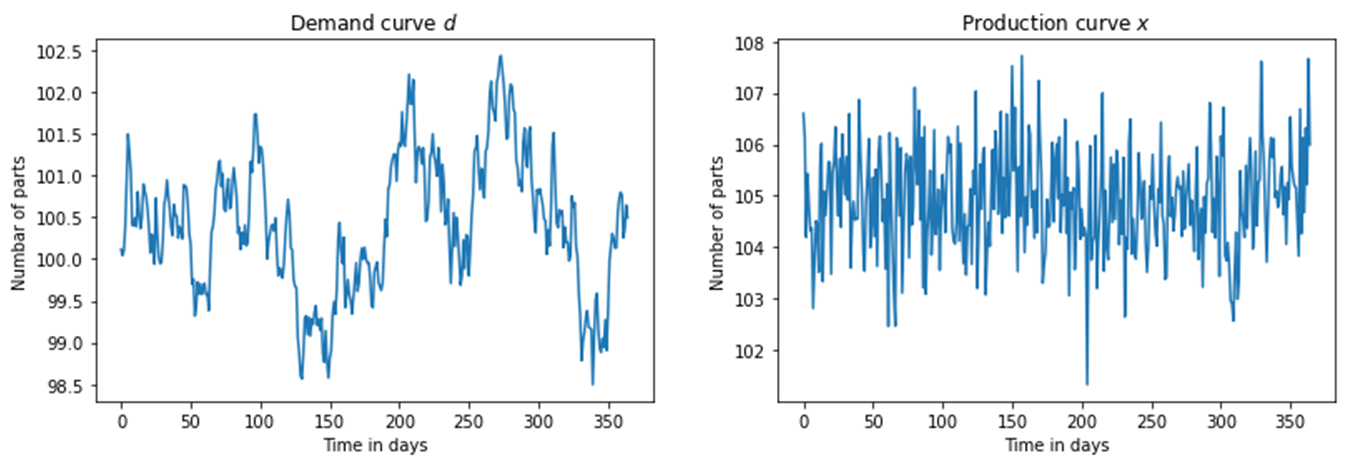
\includegraphics[width=1\textwidth]{SectionIntroduction/informationFramework_figures/fig_demandProduction.png}
\captionsetup{type=figure}
\caption{Examples of demand and production functions.}
\label{fig_demandProduction}
\end{figure}

Given $x$, $d$, and an initial inventory $q_0$, it is possible to define the inventory function $q$.

\begin{equation}
q_t=\ q_{t-1}\ +\ p_t\ -\ d_t\ 
\label{eq_physics1}
\end{equation}

The difference between the demand and production curves define the \textit{momentum} $p$ of the production node. The momentum indicates the direction in which the inventory function $q$ moves, and it is measured as the number of parts per unit of time.

\begin{equation}
p=x-d=\dot{q}
\label{eq_physics2}
\end{equation}

We identified an approach to model a supply chain using the law of physics. In particular, there is a relationship between the flows (demand $d$ and production $p$) and the inventory $q$. We can assume that some forces (may them be push or pull forces) play a role in changing the value of the inventory function $q$. Table \ref{tab_classicalMechanics} illustrates the parallelism between classical mechanics and the physics of a supply chain.

% INSERT tab_classicalMechanics
\begin{figure}[hbt!]
\centering
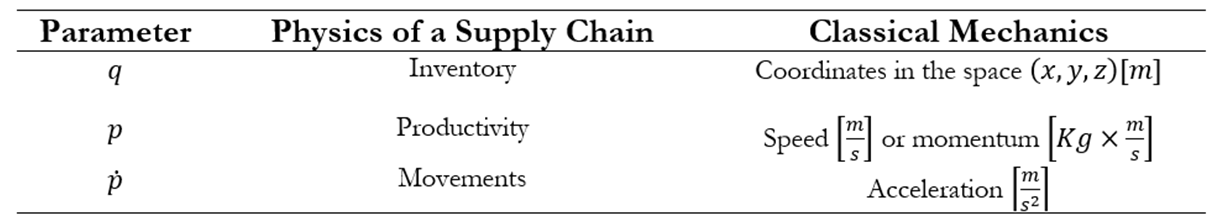
\includegraphics[width=1\textwidth]{SectionIntroduction/informationFramework_figures/tab_classicalMechanics.png}
\captionsetup{type=figure}
\caption{Examples of demand and production functions.}
\label{tab_classicalMechanics}
\end{figure}

\cite{Spearman2014} demonstrated that the energy conservation law is appliable to the physics of a supply chain to control the behaviour of the inventory curve $q$ The Lagrangian is used to express the equation of the force $\dot{p}$, representing the push and pull forces of a supply chain, i.e. the movements of the supply chain.

\begin{equation}
\dot{p}=\frac{\partial L(q,\dot{q})}{\partial q}
\label{eq_physics3}
\end{equation}

Where $L\left(q,\dot{q}\right)=\frac{1}{2}p^2-V(q)$. The Lagrangian express a difference between kinetic and potential energy. The potential energy is defined using a linear potential $V\left(q\right)=-F_0q$. This means that, as it works with the force of gravity, the perturbation of the value of the inventory depends on the value of the inventory q with a linear law. We can assume conservation of energy using the Hamiltonian principle (the Principle of Least Action). This principle states that nature always chooses the lowest energy path (i.e. the difference between kinetic and potential energy) between all the feasible ones defined by forces. The inventory function q, is then, defined from the Lagrangian as:

\begin{equation}
S\left[q\right]=\int_{t_1}^{t_2}{\ L(q,\dot{q},t)dt}=0
\label{eq_physics4}
\end{equation}

\cite{Spearman2014} shows how choosing the value of $F_0$ to control the value of inventory $q$.


\section{The information of a supply chain}
Section \ref{sect_supplyChainPhysics} demonstrated that a physical relation exists between three variables of a supply chain: the inventory $q$, the productivity $p$, and the movements $\dot{p}$. Physics is the core of science, and we can always rely on physical laws. Nevertheless, in practice, we may not have the possibility to apply these laws since data are collected with different granularities (i.e. referred to different processing nodes) or with inconsistencies. For this reason, this section introduces an original information framework to build $q$, $p$, and $\dot{p}$ using the available data. We move the focus from the physical relationship to the information relationship existing between these three functions.

\subsection{Information framework} \label{secInfoFramework}
While defining data structures to support logistics, databases are usually designed using an entity-relationship (ER) model ~\cite{Lake2013}. The focus of ER models is on the entities, i.e. the ones we defined in section \ref{secOntology}. Here we propose a different perspective, focusing on the physical logistic phenomenon, i.e. the variation in the demand $d$, production $x$ and inventory $q$ due to the forces $\dot{p}$, regardless of the entities generating these forces.\par

This change of perspective enhances the flexibility of this modelling approach since it is often difficult to collect data from all the entities involved in a supply chain and to connect them into an ER model. On the other side, the effect of the forces generated by these entities is clearly measurable on the production and demand functions.

For the sake of clarity, we abandon the dot notation, and we define:
\begin{enumerate}
    \item a movement function $M_i(t)$ to represent the forces $\dot{p}$, applied to a part $i$;
    \item a productivity function  $P_j(t)$ to represent the speed $p$ at which the forces change the value of the inventory $q$;
    \item an inventory function $I_i\left(t\right)$ representing the inventory $q$ of part $i$.
\end{enumerate}

The $M$ function has different granularity (e.g. order, vehicle, terminal, network) depending on the measurement system and the data collection system used. The most granular is a movement called by a single order $o$ of a part $i$ involving a processing node $j$ and a vehicle $v$. The function uses:

\begin{itemize}
    \item a positive value to describe the physical movement of a quantity $q$ from a processing node to a vehicle (load movement: $j\rightarrow v$);
    \item a negative value to describe a physical movement of a quantity $q$ from a vehicle to a processing node (offload movement: $v\rightarrow j$).
\end{itemize}


\begin{equation}
M_o^{j,v}(t) =\left\{
                \begin{array}{ll}
                 q & if \  t=t_{IN}, \\
                -q & if \  t=t_{OUT}, \\
                0 & otherwise.
                \end{array}
              \right.
\label{eq_movements}
\end{equation}

Where $t$ measures the time; $q$ is the quantity (e.g. the number of parts) involved in the physical movement; $t_{IN}$ is the timestamp when the part $i$ is loaded on a vehicle $v$; $t_{OUT}$ is the timestamp when it is unloaded from it.\par

The inventory function $I$ describes the inventory position (e.g. the number of parts) of a vehicle $v$ or a processing node $j$. The function $I$ is linked to $M_o^{j,v}(t)$ by aggregating the movements of single orders.\par

\begin{equation}
I_j(t) = I_j(t-\epsilon) -\sum_{i}\sum_{v}M_o^{j,v}(t) 
\label{eqInvj}
\end{equation}

\begin{equation}
I_v(t) = I_v(t-\epsilon) +\sum_{i}\sum_{j}M_o^{j,v}(t) 
\label{eqInvv}
\end{equation}

The parameter $\epsilon$ is a sufficiently small time sampling unit (e.g. a minute). It is essential to consider the initial inventory $I_j(t=0)$ and $I_v(t=0)$ to define the inventory functions correctly. Figure \ref{fig_movementsInventory} represents an example of the movements and inventory functions for a part $i$. 

% INSERT fig_movementsInventory
\begin{figure}[hbt!]
\centering
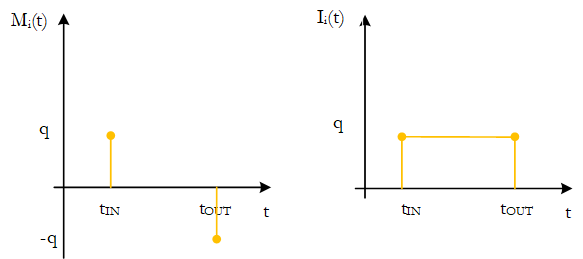
\includegraphics[width=1\textwidth]{SectionIntroduction/informationFramework_figures/fig_movementsInventory.png}
\captionsetup{type=figure}
\caption{Example of movements and inventory function.}
\label{fig_movementsInventory}
\end{figure}

The productivity function $P$ defines the motion equation of a processing node $j$, i.e. the speed of the changes in its inventory position. Two distinct $P$ functions exist to describe the loads (IN), and the offloads (OUT) speed of a processing node. The productivity function $P$ is defined, starting from the cumulative function of the movements $Q$.

\begin{equation}
Q_j^{IN}(\tau)=\sum_{i}\sum_{v}\{M_i^{j,v}|M_o^{j,v}>0,t\leq \tau \}
\label{eqQIN}
\end{equation}

\begin{equation}
Q_j^{OUT}(\tau)=\sum_{i}\sum_{v}\{M_i^{j,v}|M_o^{j,v}<0,t\leq \tau \}
\label{eqQOUT}
\end{equation}

The productivity $P$ at a time instant $t^\ast$ is given by:

\begin{equation}
P_j^{IN} (t^* )=\frac{dQ_j^{IN} (\tau)}{d\tau}\vert_{t^*}
\label{eqProdIN}
\end{equation}

\begin{equation}
P_j^{OUT} (t^* )=\frac{dQ_j^{OUT} (\tau)}{d\tau}\vert_{t^*}
\label{eqProdOUT}
\end{equation}

Movements usually have redundant information on vehicles ad processing nodes. We overcome this redundancy by splitting this information into two separate functions of inventory $I$ and productivity $P$. Productivity function, in fact, does not suffer redundancies, and it converges to a value determined by the physical asset of a terminal. \par

At this stage, we want to demonstrate the relationship between these three functions. Fro this reason, we consider the movement function at the granularity of a processing node $M_j(t)=\sum_{v}\sum_{o}{M_o^{j,v}(t)}$  and we prove the following theorem that introduces consistency rules between the functions $M_j$, $I_j$ and $P_j$ calculated with the granularity of a processing node $j$. \par

Let us consider the supply chain system as a network $G(V,A)$ where $V$ is the set of the processing nodes connected by arcs $(j,k)\in A$. Let us define a set $B$ containing the vehicles $v\in B$, travelling on the arcs $(j,k)\in A$. We define a state function $\Lambda(\tau)$ to describe the state of the network $G$ at the time instant $\tau$.   


\begin{equation}
\Lambda\left(\tau\right)=\ \left\{I_j\left(\tau\right),\ j\in V\ \bigcup{I_v\left(\tau\right),v\in}B\right\}
\label{eq_stateLambda}
\end{equation}

We demonstrate that:

\begin{theorem} \label{theor_MIP}
One of the following set of equations 
\begin{enumerate}[label=(\roman*)]
    \item $M_j(t)$
    \item $I_j(t)$
    \item $P_j^{IN} \bigcup P_j^{OUT} $
\end{enumerate}
has enough information to define the state $\Lambda$ of a logistic network. 
\end{theorem}

\begin{proof}

We demonstrate Theorem 1 by showing that the knowledge of (i), (ii), or (iii) is enough to define all the three $M$, $I$, and $P$. Statement (i) has already been demonstrated by the \ref{eqInvj}, \ref{eqProdIN} and \ref{eqProdOUT}. Statement (ii) can be proved considering the definition of $I$, since:


\begin{equation}
M_j(t)=I_j(t)-I(t-\epsilon) 
\label{eqThPart2}
\end{equation}

Given $M_j (t)$ the functions $P_j^{IN}$ and $P_j^{OUT}$ are calculated similarly to \ref{eqProdIN} and \ref{eqProdOUT}. \par
Statement (iii) can be proved considering:

\begin{equation}
Q_j^{IN} (\tau)=\int_0^\tau P_j^{IN}(t)dt
\label{eqThPart3IN}
\end{equation}

\begin{equation}
Q_j^{OUT} (\tau)=\int_0^\tau P_j^{OUT}(t)dt
\label{eqThPart3OUT}
\end{equation}

By sampling the functions $Q$ with a sampling frequency $\epsilon$ (e.g. a minute), it is possible to get the movement function.

\begin{equation}
M_j(t)=\frac{dQ_j^{IN}(t)}{dt} - \frac{dQ_j^{OUT}(t)}{dt}
\label{eqThPart3Mov}
\end{equation}

\end{proof}

The proof of Theorem \ref{theor_MIP} shows that the functions $M$, $I$ and $P$ are interconnected, and retain enough information to define the state $\Lambda$ of the network when they are measured with terminal granularity. 

\subsection{Implementation and utilisation of the framework}
The following chapters of this work start from the application of this information framework to warehouses, production and distribution system. The consistency rules between the metrics of movements, inventory and productivity, are the starting point to collect, store and analyse data leading, and to generate knowledge from this data.\par

We start with the definition of a data structure able to host movements and inventory data of a specific type of processing node. Then data-driven methodologies are proposed to build prediction models addressing node-specific problems. ER structures are designed to store both planning or actual data. In particular:

\begin{itemize}
    \item planning data, (i.e., recorded before it happens what they describe) describes how operations are planned to be performed;
    \item actual data (i.e., recorded when it happens what they describe), describes how activities were performed.
\end{itemize}

Table \ref{tab_MIPinLS} qualitatively introduces different types of data recorded on-field and used in the following sections to populate the data structure, according to the M,I,P framework.

% INSERT tab_MIPinLS
\begin{figure}[hbt!]
\centering
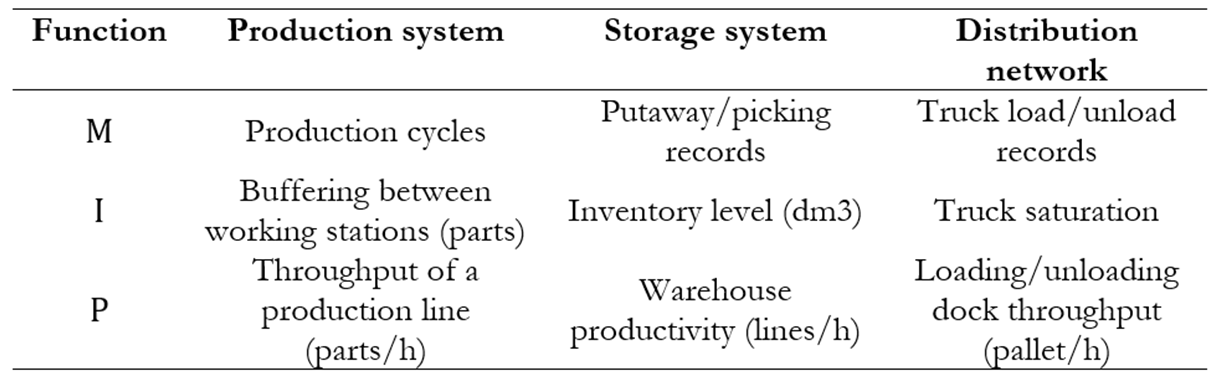
\includegraphics[width=1\textwidth]{SectionIntroduction/informationFramework_figures/tab_MIPinLS.png}
\captionsetup{type=table}
\caption{Examples of datasets connected to the functions.}
\label{tab_MIPinLS}
\end{figure}

\clearpage


%\clearpage
\bibliographystyle{ieeetr}
\bibliography{SectionIntroduction/informationFramework_ref}
\chapter{Data-driven decision making}

%citazione introduttiva
\epigraph{\textit{A data scientist must deeply know his knowledge domain.}}{}



Chapter \ref{chap_InformationFramework} introduced the entities and the metrics of a supply chain system. This book deals with these entities from a system analysis perspective (see section \ref{secSupplyChainTaxonomy}), i.e. considering the design and control alternatives to manage the operations of a distribution network, a storage system, or a production plant. These problems have been mostly addressed by decision science. The following chapters aim at identifying boundaries between decision science, and data science in the system analysis of a supply chain system. It will be remarked, as well, where data science is ready to compete with decision science to address a decision problem.\par

It is crucial to consider the knowledge domain of supply chain systems to do this job ~\cite{Stadtler2008, Hull2016}. While decision science has the ability to model each problem precisely, with instance-tailored boundaries and objective functions, we aim at designing a high-level classification of supply chain system problems. We identify patterns among similar decision problems encountered in different supply chain systems whose entities are defined by the ontology in \ref{secOntology}. Each decision pattern is identified by an id used in the following chapter as reference.\par

The following section introduces a glossary of data and information to understand the meaning of these words correctly; the classification of the decision patterns; a method to choose the right analytical technique to address a supply chain system problem, given its data, and its decision pattern; a summary of the main contributions of this book.

\section{Data Glossary}

Since this book deals with data, it is important to remark some crucial aspects. The traditional engineering modelling approach is based on intuition. The researcher observes a logistic phenomenon, makes assumptions, build a model, and fit the empirical data to the model. The data-driven approach is profoundly different since it collects data and different models fit the data, identifying the model with the best fit.\par

Our data collection activities involve multiple entities since we use a top-view perspective, looking at the system analysis. For this reason, we may have multiple data sources with redundant information, different synchronism, different granularities, different data protocols. Table \ref{tab_data_glossary} introduces the glossary explaining all these elements.

% INSERT tab_data_glossary
\begin{figure}[hbt!]
\centering
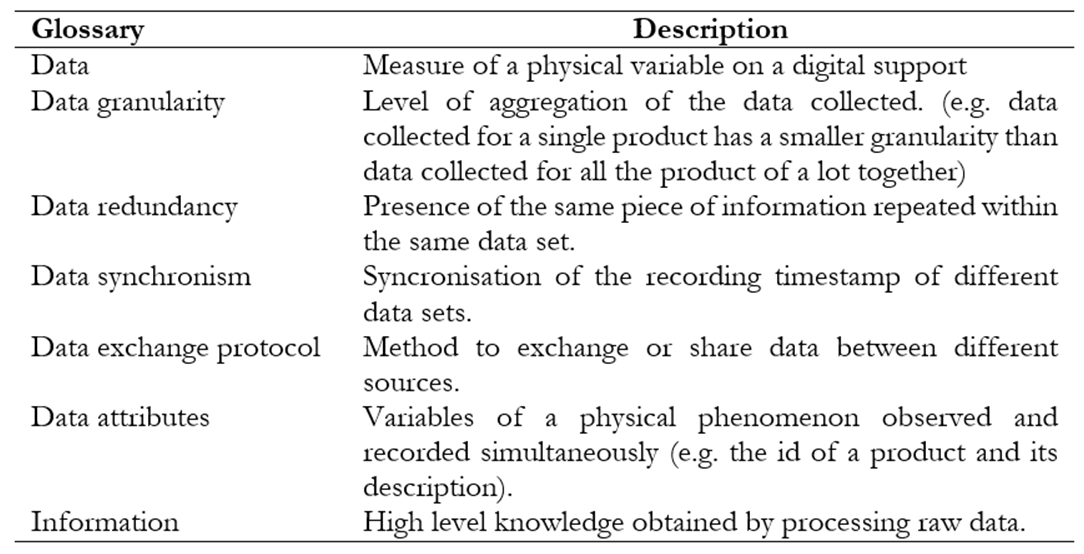
\includegraphics[width=1\textwidth]{SectionIntroduction/dataDrivenDecisions_fig/tab_data_glossary.png}
\captionsetup{type=table}
\caption{Glossary of data-related terms.}
\label{tab_data_glossary}
\end{figure}

\section{Decision patterns} \label{secDecisionPatterns}
Entities are connected with relevant strategic and control issues that must be addressed to properly organise the operations of a warehouse, production plant, or distribution system. The literature defines these issues as problems, using mathematical models. We organise these problems by introducing an original classification, with ten classes. Each class is addressable by the same branch of analytics (descriptive, explorative, predictive, or prescriptive), depending on the type of problem. 

\paragraph{Family problems (P1)}
This class of problems aims at defining homogeneous clusters of parts, to simplify the organisation of operations. Issues belonging to this class concern definitions of product families with the same production cycle (i.e. the route), and definitions of classes of stock-keeping units (SKUs) with similar characteristics (e.g. weight and volume). Descriptive and explorative analytics offer tools to assess the features of parts and to produce clusters. 

\paragraph{(Technology) Assignment problems (P2)}
This class of problems solves the assignment of parts to resources and vehicles from a high-level strategic perspective. Some examples are the assignment of SKUs to storage locations, the assignment of points of demand to trucks or the identification of the families of product to be processed by a resource (e.g. a production line or an FMS). The best configuration is found by the evaluation of every single alternative (prescriptive methodologies) or the definition of homogeneous clusters by an explorative technique.\par

Problems involving the definition of adequate technology for production nodes belong to this class and can be addressed using the same rationale. The definition of the storage system technology (storage rack with/without forward-reserve, floor stack, automated storage technology) and the identification of the level of automation in a production plant are examples of these problems. The technological choice in a distribution network (i.e. truck/rail/water/air) is neglected since it is imposed by the existent infrastructure or by political choices falling outside the domain of this research. The choice of the vehicle is solved in an operational environment with synchromodality i.e. when multiple transportation options exist for the same transportation unit (e.g. a pallet on a barge or a truck).

\paragraph{Flow problems (P3)}
This class of problems identifies how processing nodes are connected. They only exist for warehouse and production nodes since the design of the distribution infrastructure belongs to transportation science, and it is outside the domain of this research. The definition of the rationale to travel within storage racks (i.e. return or traversal policy) and the identification of paths for conveyors and forklifts in a production plant are examples of these problems. As for technology assignment problem, flow problems need prescriptive tools to identify efficient handling solutions.

\paragraph{Mechanical plant and equipment design (P4)}
This class of problems addresses engineering issues, such as the design of power plants, thermal plants, mechanical plants, lighting systems, air conditioning systems, and/or the physical designs of workbenches, material slots, and ergonomics. All these activities usually have poor historical data, and it is difficult to structure a series of previous observations of data addressing the same problem. For this reason, prescriptive models often address these problems by relying on an engineering model describing the dynamics or thermodynamics of the system.

\paragraph{Power problems (P5)}
This class of problems identifies the amount of power required for a specific resource $j$, and defines its capacity $C_j$. The storage allocation and design of areas for inbound/outbound operations are examples of power problems in a storage system. The design of the frequency of a route and service time windows at a terminal are power problems in a distribution network; the definition of the number of machines of the same type is a version of this problem in a production node. Prescriptive tools allow for solving these problems.

\paragraph{Placement problems (P6)}
A placement problem defines the identification of the proper disposition of entities (e.g. resources or set of parts) on the plant layout of a production system or storage system. Examples include the definition of a plant layout or location of a facility, the assignment and placement of SKUs to warehouse zones, the definition of the location of the facilities of a distribution network (location-allocation problem). Prescriptive and explorative techniques address these problems by clustering parts with similar behaviour (e.g. placing the same resources close to each other). 

\paragraph{Dispatching rules (P7)}
This class of problems provides rules for organising operations among the many possibilities and uncertainties that may occur in practice. The definitions of the shipping priority for transportation units and the picking policy (e.g. batching, sorting, pick and pack, single-order picking, cross-dock) for SKUs are examples of dispatching rules. In a production environment, the choice between a pull or a push policy is another dispatching rule. Dispatching rules affect the level of the work in process, size of the lots, and rationale for satisfying the market demand (i.e. pull/push). The definition of these rules requires a prescriptive model.

\paragraph{Performance assessment (P8)}
This class of problem is deliberately descriptive. It aims to describe the system $G$, its entities (i.e. parts, resources and vehicles), and its processes (i.e. jobs and routes). Data science offers tools to approach this type of problem, as the results are obtained exclusively using descriptive and explorative tools for evaluating the log data from a storage system, production system, or distribution network.

\paragraph{Workload predictions (P9)}
This class of problems aims at forecasting the values of relevant variables regarding a product or a process in the future. The predictions are influenced by market demand. Hence, predictions consider the number of parts (e.g. SKUs, containers, or products) which will be processed by a system $G$ in the near future. The estimate of the number of parts leads to the prediction of other relevant process variables (e.g. the speed of a machine, or number of operators required to perform activities).

\paragraph{Operations management (P10)}
This class of problems prescribes how to act within given circumstances to perform operations. This problem always involves a prescription, e.g. the definition of a sequence of products to process on a machine (job scheduling), or the sequence of locations to visit from a truck in a distribution system or a forklift in a warehouse system. Prescription tools can approach these problems when the input data are consistent and compliant with their hypotheses. In particular situations, predictive and explorative tools may be used to address the problem as well. For example, when processing a single part to assign to a resource in an online version of the problem (e.g. a last-minute order to assign to a production machine), a prediction or clustering model based on robust data can solve the assignment, given the current state of the system $G$.

\section{Decision trees}
Once the class of analytics (i.e. descriptive, explorative, predictive, or prescriptive) for solving a problem has been defined, it is necessary to identify the technique for obtaining a solution. Different methodological paths exist to solve a problem $P$, depending on:

\begin{enumerate}
    \item the need to set up decision variables D to solve the problem (e.g. in prescriptive analytics);
	\item the availability of measurements on previous realisations of the solution;
	\item the completeness and the accuracy of the realisation dataset; and
	\item the knowledge on the boundary conditions of $X$.

\end{enumerate}

We introduce three original decision trees to identify these paths, and to guide the decision-maker in the definition of the proper technique to address a problem. Decision trees focus on descriptive, predictive, and prescriptive analytics, whereas exploratory analytics appears in some branches of the other trees.

\subsubsection{Descriptive decision tree}
This tree aims at the description of a variable $y$ as a random variable; $y$ is usually a KPI metric, and there are no decision variables $D$ to set up. Sometimes, it is impossible to directly measure a variable on-field (e.g. often when $y$ is a cost). In these cases, it is necessary to link the value of $y$ with a kinematic model $y=f(X)$, based on a set of measurable variables $X$ that are inputs of a motion equation $f$. The variables $X$ usually describe the movements of a logistical process (e.g. the path travelled by a truck on a road or by a forklift within a plant). Once $f$ is defined, a numerical simulation (e.g. Monte Carlo simulation) allows for investigating the behaviour of $y$, depending on the distribution of $X$ and on the tuning parameters of the kinematic model. When $y$ is measurable but the dataset presents different data sources with different levels of accuracy, Bayesian statistics can be used to infer the properties of $y$ by leveraging its estimate and considering the reliability of each input data source. Otherwise, the inferential statistic is appropriate when the data are from a single source, and there are no measurements $Y$ of other variables linked to $y$. When a dataset $Y$ containing observations of a set of variables connected to $y$ is available, explorative analytics (i.e. clustering) is suitable for investigating the correlations between the variables and improving the knowledge of the decision maker regarding the important variables affecting the process. Figure \ref{fig_describe_tree} introduces the descriptive decision tree, and illustrates the decision steps identified above.

% INSERT fig_describe_tree
\begin{landscape}
\thispagestyle{empty}
\begin{figure}[hbt!]
\centering
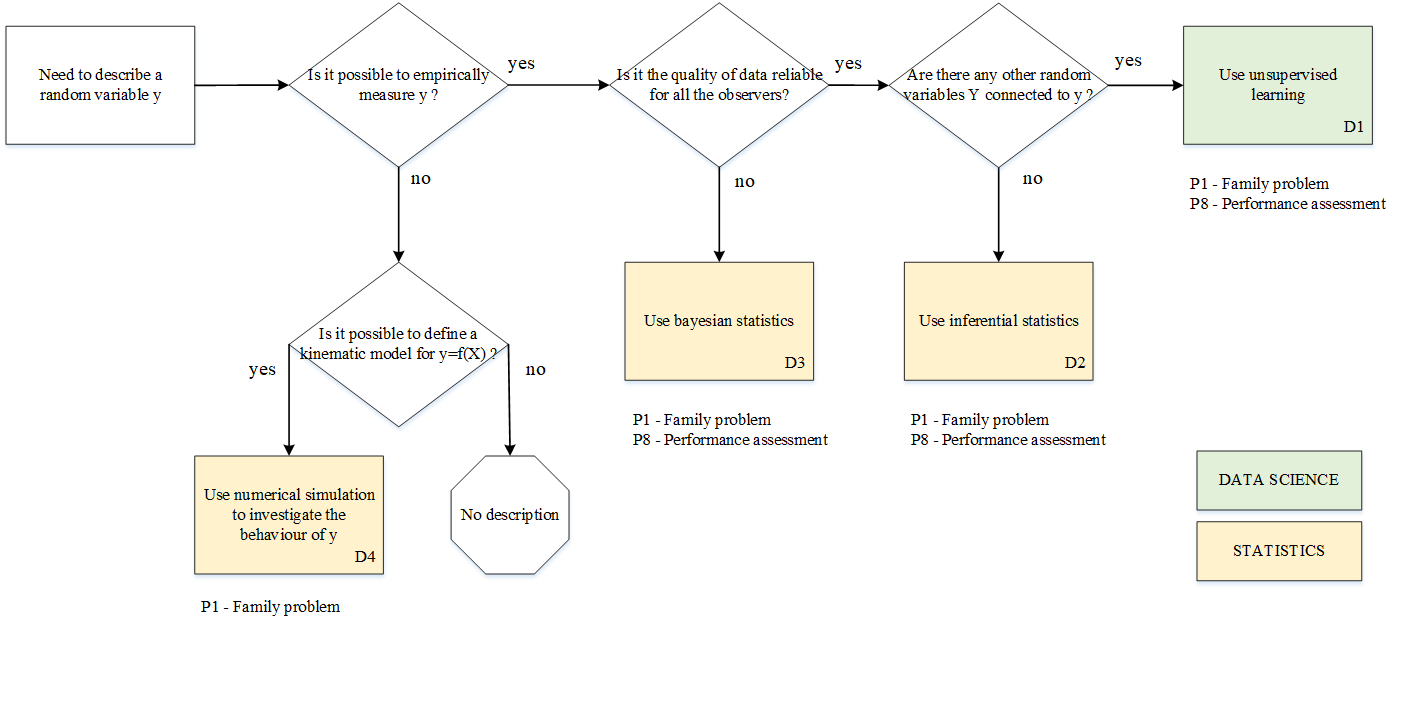
\includegraphics[width=1.5\textwidth]{SectionIntroduction/dataDrivenDecisions_fig/fig_describe_tree.png}
\captionsetup{type=figure}
\caption{Decision tree for descriptive purposes.}
\label{fig_describe_tree}
\vfill
\end{figure}
\end{landscape}




\subsubsection{Predictive decision tree}

This tree aims at forecasting future realisations of a variable $y$, given its description as a random variable. For this reason, there are no variables $D$ to set up (except for the hyperparameters of some forecasting models). The ability to empirically measure the variable $y$ is a key branch of the decision tree. If the variable cannot be measured directly (e.g. the inventory position of a truck while travelling), the only other option is to define a kinematic model to estimate its value (e.g. estimating the inventory using loading and unloading records). Without a kinematic model and/or a direct measurement, it is impossible to make predictions. When the variable can be measured but the measures are incomplete (e.g. a small subset of the dataset), explorative clustering techniques can be used to extend the properties measured for the small sample to the entire population $\widetilde{y}$ (e.g. from a subset of parts to an entire product family). In this case, it is necessary to have a validation dataset $\hat{y}$ associated with the values of $\widetilde{y}$. If a validation dataset is not available, the kinematic model remains the sole alternative for obtaining an estimate. Otherwise, it is possible to set a prediction model. When there are no other variables $Y$ associated with $y$, time-series forecasting (e.g. decomposition, Fourier analysis, autoregressive integrated moving average (ARIMA) models) can be used to make predictions. When a dataset of variables $Y$ associated with $y$ is available, supervised machine learning models can lead to more accurate predictions. Figure \ref{fig_predict_tree} illustrates the decision tree, along with the decision steps identified above.

% INSERT fig_predict_tree
\begin{landscape}
\thispagestyle{empty}
\begin{figure}[hbt!]
\centering
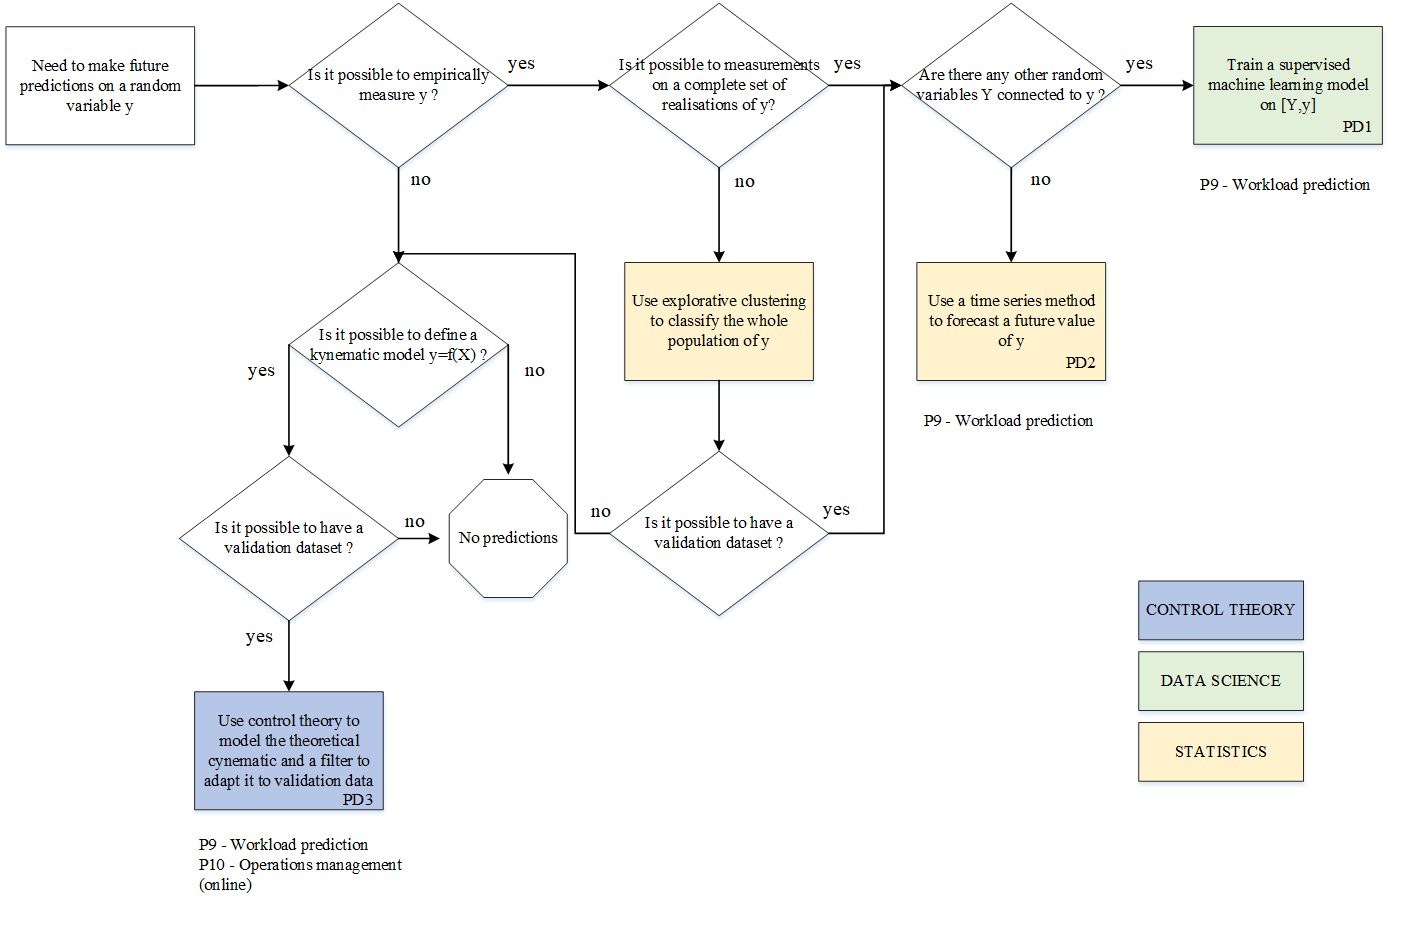
\includegraphics[width=1.5\textwidth]{SectionIntroduction/dataDrivenDecisions_fig/fig_predict_tree.png}
\captionsetup{type=figure}
\caption{Decision tree for predictive purpose.}
\label{fig_predict_tree}
\vfill
\end{figure}
\end{landscape}

\subsubsection{Prescriptive decision tree} \label{secPrescriptiveDecisionTree}
When addressing prescription problems, it is necessary to identify a set of decision variables $D$, such that an objective on $y$ can be reached (e.g. a cost can be minimised). As for the previous trees, when $y$ cannot be directly measured, it is necessary to define a kinematic model $y=f(D)$. If no validation dataset $\hat{y}$ is available, there is no scientific way to set $D$. Otherwise, control theory can help to adapt the kinematic model to realisations in the real world. The optimal solution is obtained by using mathematical minimisation (e.g. derivatives) on the motion equations of the system. When measurements are available on a subset of realisations of $y$, unsupervised clustering is used to extend the properties of the observed dataset with a clustering function $y=g(D)$. If the problem is an assignment problem, the clustering boundaries $g$ may be sufficient to solve the problem (e.g. assignment of parts to processing nodes); otherwise, it is necessary to enumerate all of the alternatives and to select the best one. When a dataset with observations for all of the entities is available and it is possible to define a feasibility region for any value of $y$, optimisation should be used. Figure \ref{fig_prescribe_tree} presents the decision tree, along with the decision steps identified above.

% INSERT fig_prescribe_tree
\begin{landscape}
\thispagestyle{empty}
\begin{figure}[hbt!]
\centering
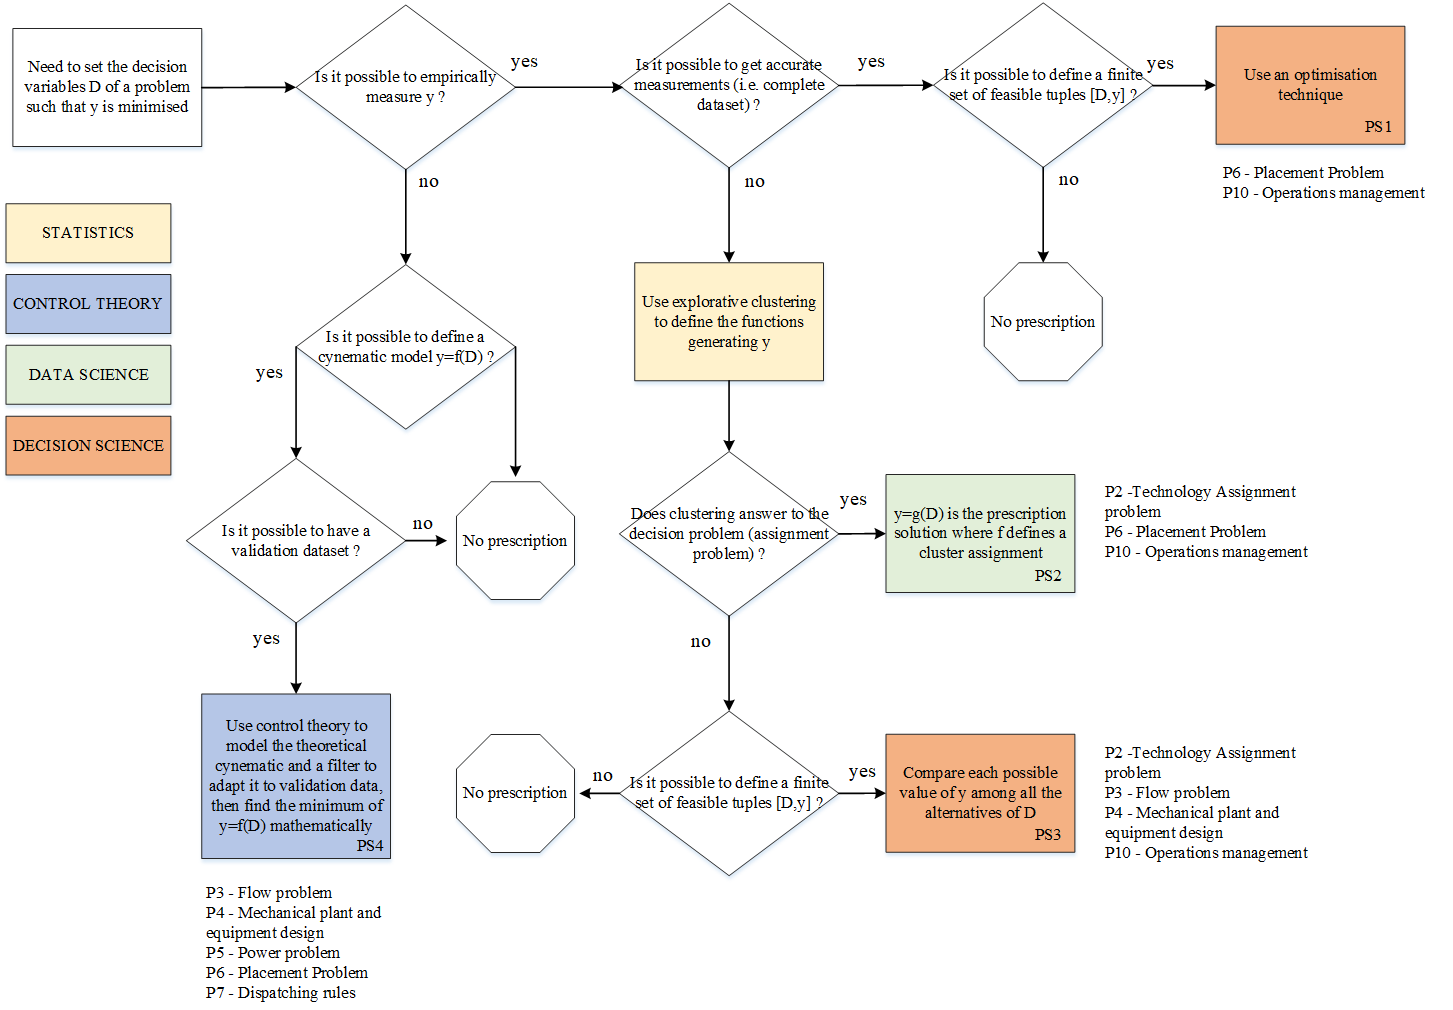
\includegraphics[width=1.5\textwidth]{SectionIntroduction/dataDrivenDecisions_fig/fig_prescribe_tree.png}
\captionsetup{type=figure}
\caption{Decision tree for prescriptive purpose.}
\label{fig_prescribe_tree}
\vfill
\end{figure}
\end{landscape}



The resulting classification of problems, analytics, and solving techniques is introduced in Table \ref{tab_problem_classification}. Each row of the table refers to a problem within its system domain (i.e. warehouse/production plant/distribution system). It identifies the type of decision (design or control) and the entities involved (e.g. part, vehicle). The right side of the table describes the classes of analytics that address the problem, and the methodologies for obtaining a solution (according to the labels used in the decision trees). For example, the first row of the table addresses the family problem (P1) in warehousing systems. This is a design decision involving the definitions of clusters of SKUs. SKUs are, then, the entities involved in being modelled as parts in the ontology. The problem is addressable by using descriptive or explorative methodologies, labelled as D1, D2, and D3 in the decision trees.


% INSERT tab_problem_classification
\begin{landscape}
\thispagestyle{empty}
\begin{figure}[hbt!]
\centering
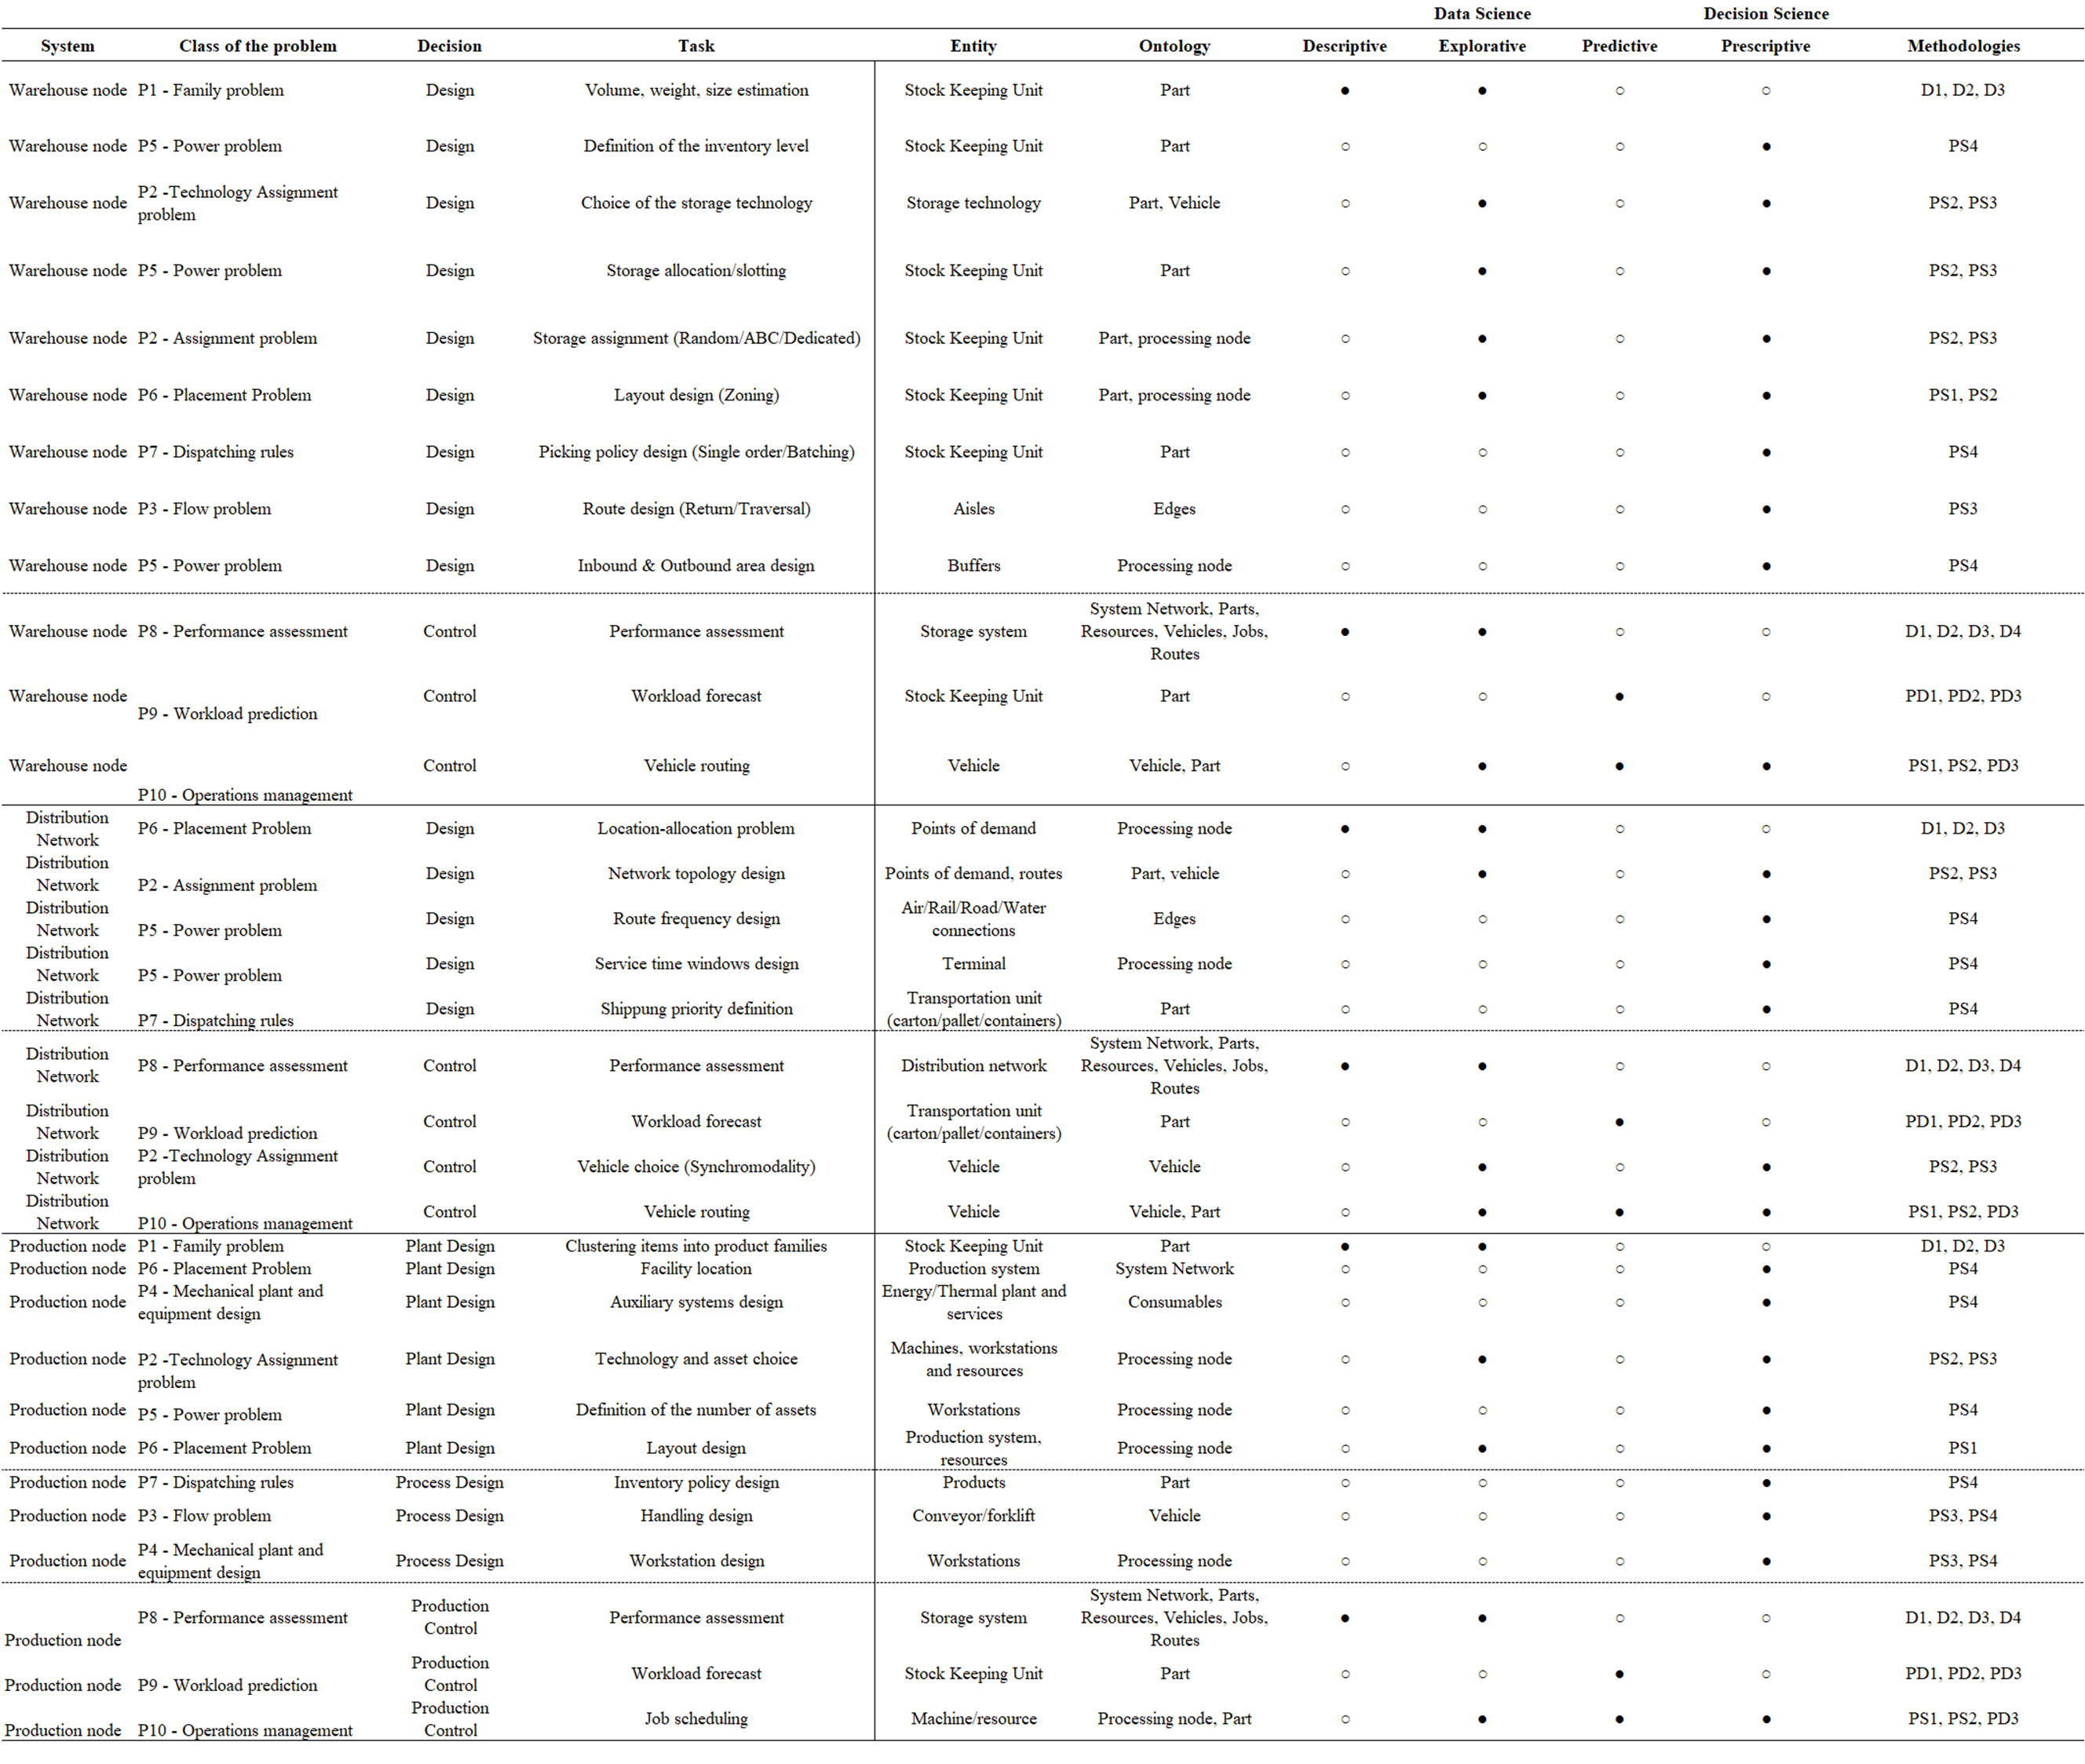
\includegraphics[width=1.3\textwidth]{SectionIntroduction/dataDrivenDecisions_fig/tab_problem_classification.png}
\captionsetup{type=table}
\caption{Definition of the problems for warehouse nodes, production nodes and distribution networks.}
\label{tab_problem_classification}
\vfill
\end{figure}
\end{landscape}

\section{Main contributions of this book}
Chapter \ref{chap_InformationFramework}, and the previous paragraph of this chapter, introduced a new method to structure data, and precise pattern to identify the analytical approach to solve a problem. The remainder of this book shows how to apply these elements to distribution networks, storage systems, and production plants.\par

In particular, we focus on the data-driven models presented in part II to show how to learn information from a dataset; while part III, IV, and V shows what information can be learnt from logistics and operational data.\par

We explore the role of data in logistics and operations research. The research, according to the first three paradigms, involves the design of a model and the optimisation of the modelled system using the models’ parameters. Here we use the fourth science paradigm; for this reason, the solely modelling activity involves the definition of consistency rues between data (i.e. the information framework introduced in chapter \ref{chap_InformationFramework}). For this reason, each of the following sections proposes relational, and non-relational data structures to host data from a specific industrial domain (i.e. warehousing, transportation and production). We will show that, if data are stored correctly, it is possible to define consistency rules to get the highest information even when the input data is incomplete. \par

Another important contribution regards the way we do research. Researchers must do experiments. Doing experiments at a system level is hard since it is impossible to build a lab containing a globally distributed supply chain. For this reason, we create virtual environments using digital twins of the entities of a supply chain. Then, we do experiments on these virtual entities. Data define the entities while scripts of code do the experiments on these entities. Our research becomes reproducible since the scripts can be run many times with different input data supporting the generalisation of our research. These scripts implement the analytics, that is the technology we want to explore and test in this research. There are two groups of scripts implemented within the virtual laboratory: general-purpose, and problem-oriented scripts.\par

General-purpose scripts implement general-purpose methods, i.e. pieces of code based on data-driven approaches that are not necessarily linked to the field of logistics and operation. All the methods illustrated in part II belong to this class of scripts.\par

Problem-oriented scripts find the solution of a problem by using a decision-pattern illustrated in \ref{secDecisionPatterns}, and may combine many general-purpose scripts. These methods are presented in part III, IV, V. \par

Another type of script manages the flow of data from the industrial data sources to the other type of scripts. Figure \ref{fig_data_flow} illustrates the flow of data. 

% INSERT fig_data_flow
\begin{figure}[hbt!]
\centering
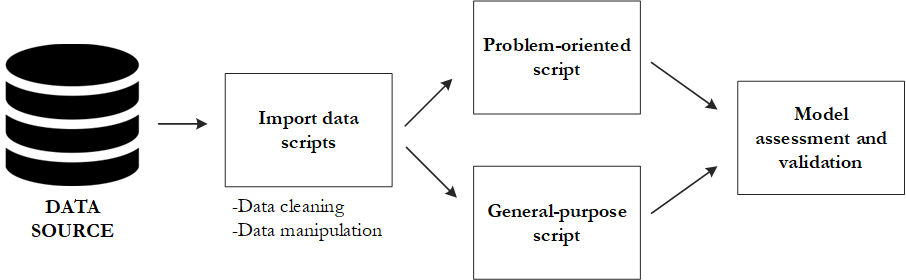
\includegraphics[width=1\textwidth]{SectionIntroduction/dataDrivenDecisions_fig/fig_data_flow.png}
\captionsetup{type=figure}
\caption{Data flow between scripts.}
\label{fig_data_flow}
\end{figure}

To support the research community in the field of supply chain systems with robust methods, and data structure, problem-oriented and general-purpose scripts are written using python ~\cite{Lee2015}, the most used programming language nowadays, and distributed with an open-source licence, according with the open-science mission indicated by the European Union ~\cite{Parliament2019}.\footnote{The package logproj contains general-purpose, and problem-oriented scripts \href{https://github.com/aletuf93/logproj}{here}.}

From a research perspective, we can state several research questions addressed by the contents of this book.

\textit{RQ1: Which data are needed to solve a problem in the field of logistics and operations?}\bigskip

\textit{RQ2: how to collect, organise, preprocess and manipulate this data?}\bigskip

\textit{RQ3: which method should be used to address an issue in the field of logistics and operations?}\bigskip

\textit{RQ4:  when the data-driven approach is recommendable to address a problem in the field of logistics and operations?}\bigskip

The remainder of this book  is organised as follows. Part II introduces and clarifies all the math, statistics and the basic models which will be applied in this book. Part III, IV and V are dedicated to a logistic system, i.e. storage nodes, distribution networks, and production plants. Each part has a similar structure illustrating:
\begin{itemize}
    \item The design of a diagnostic model to assess the entities and the metrics of a logistics system;
    \item The design of a relational data structure to store planned and actual logistics/operations data;
    \item The design of a non-relational data structure to store planned and actual logistics/operations data;
    \item Model-driven methods to address control issues of the logistic system;
    \item Data-driven methods to address control issues of the logistic system;
    \item Model-driven methods to address design issues of the logistic system;
    \item Data-driven methods to address design issues of the logistic system.
\end{itemize}





%\clearpage
\bibliographystyle{ieeetr}
\bibliography{SectionIntroduction/dataDrivenDecisions_ref}





%part 2
\part{LET'S MATH}

\chapter{Logical Modelling} \label{chapLogicalModelling}

%citazione introduttiva
\epigraph{\textit{All models are wrong, but some are useful.}}{George E. P. Box}

This book part is about math. Nevertheless, before deepening into math, it is necessary to mention the Logic, another important branch of science deeply connected with math. The Logic was the main character of the philosophical debate in ancient Greece. Aristotle was the first to set the rules of the Logic as we study nowadays \cite{Aristoteles}. \par

Today we study the Logic by using the truth table and the logical operator (i.e. $AND$, $OR$, $NOT$). These simple operations on zero and ones are performed on any CPU allowing from simple calculations to the moon landing, to machine learning and artificial intelligence. Every input or output of a computer is processed by using the rules of the logic. \par

Logical modelling is crucial for all the STEM disciplines (science, technology, engineering and mathematics) to identify a deterministic connection between the input and the output of a phenomenon. Logic permits to STEM researchers to build models based on their intuitions. These models can be validated or not by using math and statistics. Nevertheless, it is necessary to remember that all models are wrong. Models approximate reality, but they are not reality. For this reason, they are wrong.\par

Models help to understand how reality works. If you can understand reality, you can control, and change it. This fact is actual in the field of logistics and operations, whose environment involves thousands of resources, assets, goods and tasks. In this chapter, we use the logic to model and connect these entities aiming at the understanding of complex operational environments.\par 

\section{Business Process Model and Notation} \label{secBPMN}
Literature introduces many notations for modelling a business process. In this work, we introduce the Business Process Model and Notation (BPMN) that results adequate, when applied to the modelling of logistics and operational processes \cite{OMG1998}. The BPMN uses a number of predefined symbols to model entities, flows, resources and activities of any business process. The full notation requires hundred of pages of details, but the main elements (see Figure \ref{fig_BPMN}) are three \cite{White2004}:

\begin{itemize}
    \item Event: it is represented by a circle and is something that “happens” during a business process. These Events affect the flow of the process and usually have a cause (trigger) or an impact (result). 
    \item Activity: it is represented by a rounded-corner and is a generic term for work that company performs. 
    \item Gateway: it is represented by a diamond and is used to control the divergence and convergence of flows as a logic gate.

\end{itemize}

% INSERT fig_bpmn
\begin{figure}[hbt!]
\centering
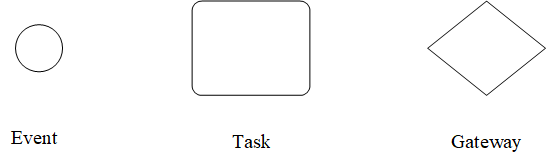
\includegraphics[width=0.8\textwidth]{SectionLetsMath/logicalModelling_figures/fig_BPMN.png}
\captionsetup{type=figure}
\caption{Main elements of a BPMN.}
\label{fig_BPMN}
\end{figure}

The following sections of this work identify the resources, asset, tasks and goods to associate with each of these elements. Figure \ref{fig_es_BPMN} illustrates an example of a BPMN to describe the operations of a port terminal.\par 

% INSERT fig_es_bpmn
\begin{landscape}
\thispagestyle{empty}
\begin{figure}[hbt!]
\centering
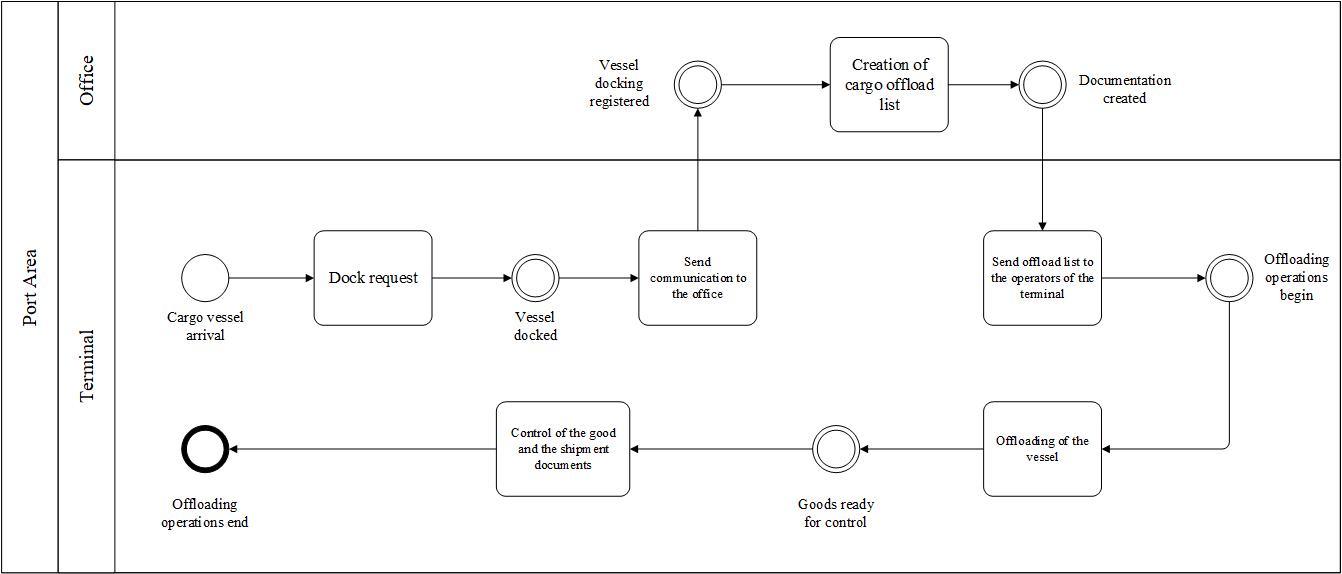
\includegraphics[width=1.3\textwidth]{SectionLetsMath/logicalModelling_figures/fig_es_BPMN.png}
\captionsetup{type=figure}
\caption{an example of a BPMN applied to the logistics of a port terminal.}
\label{fig_es_BPMN}
\vfill
\end{figure}
\end{landscape}

An additional logistic feature of the BPMN is represented by the possibility of georeferencing tasks and events. Using this method, the physical location of each activity is identified. In addition, it is possible to annotate the responsible of the activity. The BMN allows tracking the physical and information flows of logistics operations qualitatively, by introducing logical rules on the events and gateways leading to the tasks.

%\clearpage
\bibliographystyle{ieeetr}
\bibliography{SectionLetsMath/logicalModelling_ref}

\chapter{Elements of probability and statistics}{Let math do its work}

This work comes with the idea that probability and statistics can solve the majority of the problem from logistics and operations. Unfortunately, many logistics and operations manager forgot about the superpowers of statistics. Software developers do the same while deploying warehouse management systems (WMS), transportation management system (TMS) and manufacturing execution system (MES). For this reason, this chapter reviews the most essential elements of statistics and probability upon which are the base of the method implemented in the following chapters. 

\section{Probability Theory}
Probability theory aims at defining the behaviour of a variable (let us call it random variable) whose value is not deterministic. A random variable describes the realisations of an event whose outcomes are not static. Any phenomenon measured on-field is describable by a random variable. Flipping a coin is an event having two outcomes (heads or tails); a random variable can be used to describe the outcome (e.g. the expected number of heads over many flips). Operations and logistics management are based on many quantities measured on-field (e.g., time and motion, efficiency, productivity, as already introduced in Chapter \ref{chap_InformationFramework}). Random variables can be used to describe all these variables. 

Switching to math, we can define a series of $n$ observations recording the values of $n$ different realisations of the event described by the random variable $X$. In practice, we use the $n$ empirical observations to infer the properties of the random variable $X$. A random variable $X$ is fully defined by:
\begin{itemize}
    \item 	a probability density function (PDF) $f_X (x)$, or
    \item 	a cumulative distribution function (CDF) $F_X (x)$ defined as follows.
\end{itemize}

\begin{equation}
f_X\left(x\right)=prob\{X=x\}
\label{eq_pdf}
\end{equation}

\begin{equation}
F_X\left(x\right)=prob\{X\le x\}
\label{eq_cdf}
\end{equation}

The probability theory is based on the knowledge of the CDF or PDF of a random variable $X$. As previously stated, one out of the two functions is enough to fully define $X$ since $f$ and $F$ are linked by the following equation.

\begin{equation}
F_X(x)=\int_{-\infty}^{+\infty}{f_X\left(t\right)\ dt}
\label{eq_cdfIntegralPdf}
\end{equation}

Probability theory defines many “famous” probability functions where $f$ and $F$ are defined on a continuous domain by using closed-form equations. The Gaussian, exponential, uniform, beta, Weibull distributions are examples of continuous probability distributions. Discrete distributions as the binomial and Poisson are used to define a discrete realisation of an event (e.g. heads or tails, '0' or '1'). In practice, a researcher tries to find the best fit between a series of $n$ realisations collected on-field and a “famous” probability distribution with known $f$ and $F$. When he/she finds an adequate fit, the probability distribution models the behaviour of the random variable and can be used to infer relevant information on the observed event.\par

In practice, we interpret the as a frequency analysis (i.e. the histogram) of the random variable $X$. On the other side, the CDF measures the relative importance of every single observed value cumulated to all the previous. Figure \ref{fig_empiricalPdfCdf} shows the empirical and the best-fit PDF and CDF of a sample with $n=200$ observations.\footnote{The source code of Figure \ref{fig_empiricalPdfCdf} is available \href{https://github.com/aletuf93/logproj/blob/master/examples/01_elemStat/01.\%20Probability\%20Theory.ipynb}{here}.
}

% INSERT fig_empiricalPdfCdf
\begin{figure}[hbt!]
\centering
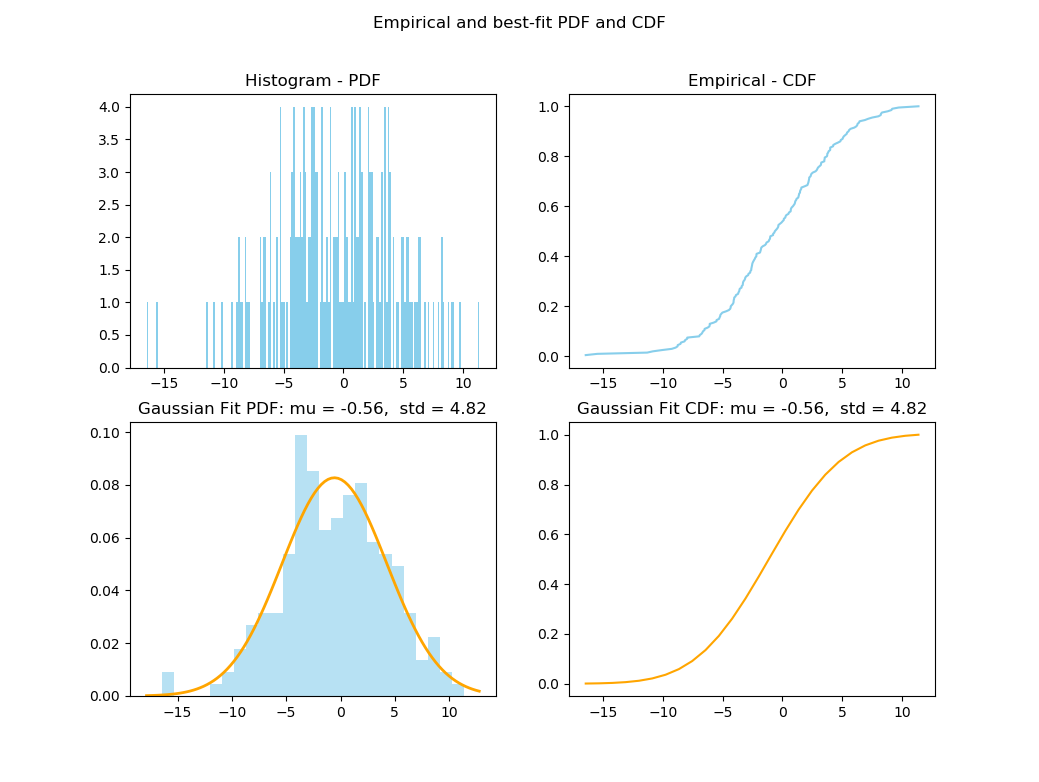
\includegraphics[width=0.8\textwidth]{SectionLetsMath/elemStat_figures/fig_empiricalPdfCdf.png}
\captionsetup{type=figure}
\caption{Empirical and best-fit probability distribution}
\label{fig_empiricalPdfCdf}
\end{figure}

\subsection{Statistical Moments}
As stated before, it is of our interest to infer properties on the random variable to understand the realisations of the related event. Statistical moments are properties that aim at parametrising the shape of a PDF. Let us define the moment of order $m$ as:

\begin{equation}
E\left[\left(x\right)^m\right]=\int_{-\infty}^{+\infty}f\left(x^m\right)dx
\label{eq_momentOfOrderm}
\end{equation}

and the central moment of order m, as:

\begin{equation}
M_m=E[\left(x-\mu\right)^m]
\label{eq_centralMomentOfOrderm}
\end{equation}

The moment of the first order is called \textit{mean} (or expectation) of the probability distribution, generally indicated using the Greek letter $\mu=E[(x)]$.\par

The central moment of the second order is called variance, and it quantifies how much the observations are far from the mean value $\mu$ of the distribution. The variance is represented by $\sigma^2$.We can express the value of $\sigma^2$  by using equation
\ref{eq_momentOfOrderm}.
\begin{equation}
    \label{eq_deploymentVariance}
    \begin{split}
    \sigma^2 & =\ E\left[\left(x-\mu_x\right)^2\right]\\
    & =\int_{-\infty}^{+\infty}\left(t-\mu\right)^2f_xdt=E\left[x^2+\mu^2-2x\mu\right]\\
    & =E\left(x^2\right)+\mu^2-2\mu^2\\
    & =E\left(X^2\right)-\mu^2
    \end{split}
\end{equation}
Usually, we take care of $\sigma=\sqrt{\sigma^2}$ since it has the same unit of measure of $\mu$.\par

Other important central moments (order 3 and 4) are used to describe the shape of a PDF:
\begin{itemize}
    \item $\frac{M_3}{\sigma^3}\ $ is called \textit{skewness};
    \item $\frac{M_4}{\sigma^4}\ $  is called \textit{kurtosis} or \textit{flatness}.
    
\end{itemize}

% INSERT fig_skewnessKurtosis
\begin{figure}[hbt!]
\centering
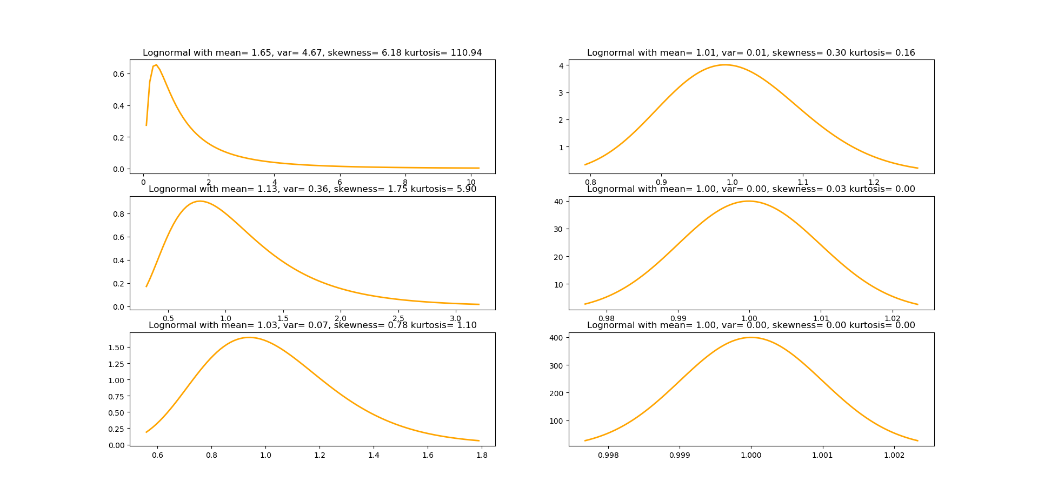
\includegraphics[width=1\textwidth]{SectionLetsMath/elemStat_figures/fig_skewnessKurtosis.png}
\captionsetup{type=figure}
\caption{Skewness and kurtosis of a lognormal distribution.}
\label{fig_skewnessKurtosis}
\end{figure}

Figure \ref{fig_skewnessKurtosis} presents an example of skewness and kurtosis of different distributions (here we use the lognormal). Skewness describes how the mode $M$ of the distribution is far from the mean $\mu$ (positive skewness when $M<\mu$ and negative skewness when $M>\mu$). Kurtosis defines the tailedness of the distribution, higher the kurtosis, higher the relevance of the tails of the distribution.\footnote{The source code of Figure \ref{fig_skewnessKurtosis} is available \href{https://github.com/aletuf93/logproj/blob/master/examples/01_elemStat/01.\%20Probability\%20Theory.ipynb}{here}.
}

\subsection{Covariance and Correlation} \label{secCovarianceCorrelation}
Often, it is necessary to compare the behaviour of two random variables to understand if their related events are somehow correlated. The covariance function $cov(X,Y)$ measures how much two random variables vary together.

\begin{equation}
cov\left(X,Y\right)=E\left[\left(X-E\left[Y\right]\right)\left(Y-E\left[Y\right]\right)\right]=E\left[XY\right]-E[X]E[Y]
\label{eq_covariance}
\end{equation}

The correlation between two random variables is a scalar number defining a measure of their statistical association. The correlation between two random variables is measured normalising the covariance to $\rho_{X,Y}$.

\begin{equation}
\rho_{X,Y}=\frac{cov(X,Y)}{\sigma_X\sigma_Y}
\label{eq_correlation}
\end{equation}

Measuring the correlation between variables is extremely important to evaluate their information content. If two variables are completely correlated (or uncorrelated), their information content is entirely defined by a single of them. Scatterplots are used to visualise correlations. Figure \ref{fig_irisCorrelation} presents an example from the famous \textit{iris dataset}. This dataset is largely used in machine learning examples, and it contains 50 samples for each of the three species of the iris flower (\textit{iris setosa}, \textit{iris virginica} and \textit{iris versicolor}). For each sample, the dataset maps the sepal and petal length and width. A high positive correlation can be easily identified between the variables \textit{petal\_len} and \textit{petal\_wid}.

% INSERT fig_irisCorrelation
\begin{figure}[hbt!]
\centering
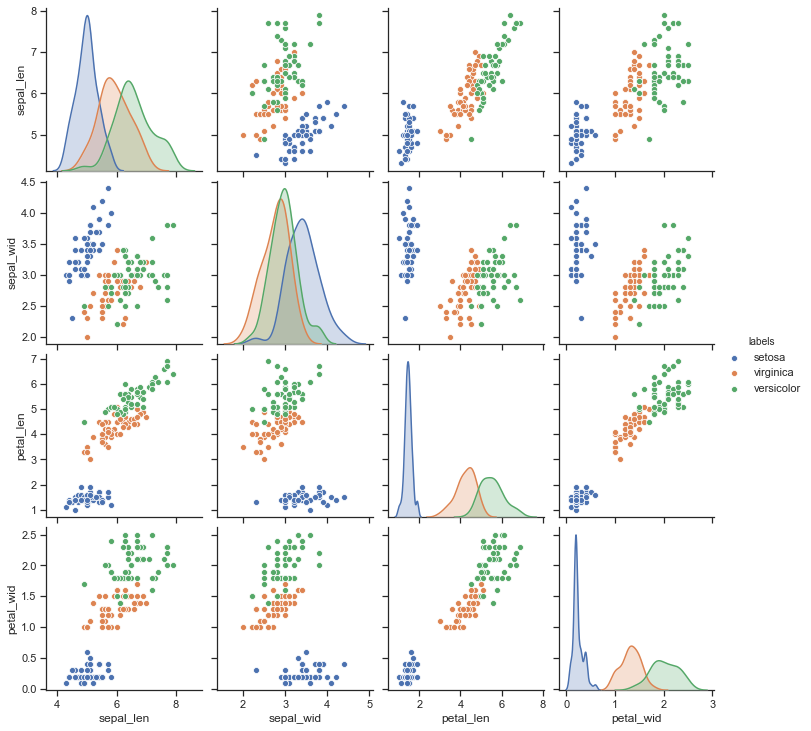
\includegraphics[width=1\textwidth]{SectionLetsMath/elemStat_figures/fig_irisCorrelation.png}
\captionsetup{type=figure}
\caption{Scatterplot of the iris sample dataset.}
\label{fig_irisCorrelation}
\end{figure}

Sometimes, it may be interesting to evaluate how much a single random variable varies with itself. This is the case of a time series that may have some seasonal components. The autocovariance is introduced to meet this goal. It measures how much a random variable varies with itself after some lag $k$ (e.g. a time lag in a time series).

\begin{equation}
\gamma_k=cov\left(X_t,X_{t-k}\right)=E\left[\left(X_t-\mu_t\right)\left(X_{t-k}-\mu_{t-k}\right)\right]-\mu_t\mu_{t-k}
\label{eq_autocovariance}
\end{equation}

Similarly to the variance, it is possible to define a global autocorrelation function (ACF) $\rho_k$ measuring the correlation of a variable $X$ with itself after a time lag $k$. This function expresses the linear dependence between the random variable observed at time $t$ and itself observed at time $t-k$.

\begin{equation}
\rho_k=corr\left(X_t,X_{t-k}\right)=\frac{E[(X_t-\mu_t)(X_{t-k}-\mu_{t-k})]}{\sqrt{Var(X_t)Var(X_{t-k})}}
\label{eq_ACF}
\end{equation}

A partial autocorrelation function (PACF) $\phi_{kk}$ is introduced to measure the linear dependence between the random variable observed at time t and itself observed at time $t-k\ $ without taking into account the intermediate correlations (i.e. $\phi_{kk}$ does not consider the dependence between $X_t$ and $X_{t-1}$ ; $X_t$ and $X_{t-2}$ ; ... ; $X_t$ and $X_{t-k+1}$).

\begin{equation}
\phi_{kk}=Corr(X_t,X_{t-k}|X_{t-1},X_{t-2},\ldots,X_{t-k+1})
\label{eq_PACF}
\end{equation}

Figure \ref{fig_ACFPACF} illustrates a seasonal time series with its ACF and PACF. ACF and PACF of the series evidence that autocorrelation of the realisations exists after about five time lags. Additional details on the use of this information for time series analysis are introduced in Section \ref{secTimeSeries}.\footnote{The source code of Figure \ref{fig_ACFPACF} is available \href{https://github.com/aletuf93/logproj/blob/master/examples/02.\%20Time\%20Series.ipynb}{here}.}

% INSERT fig_ACFPACF
\begin{figure}[hbt!]
\centering
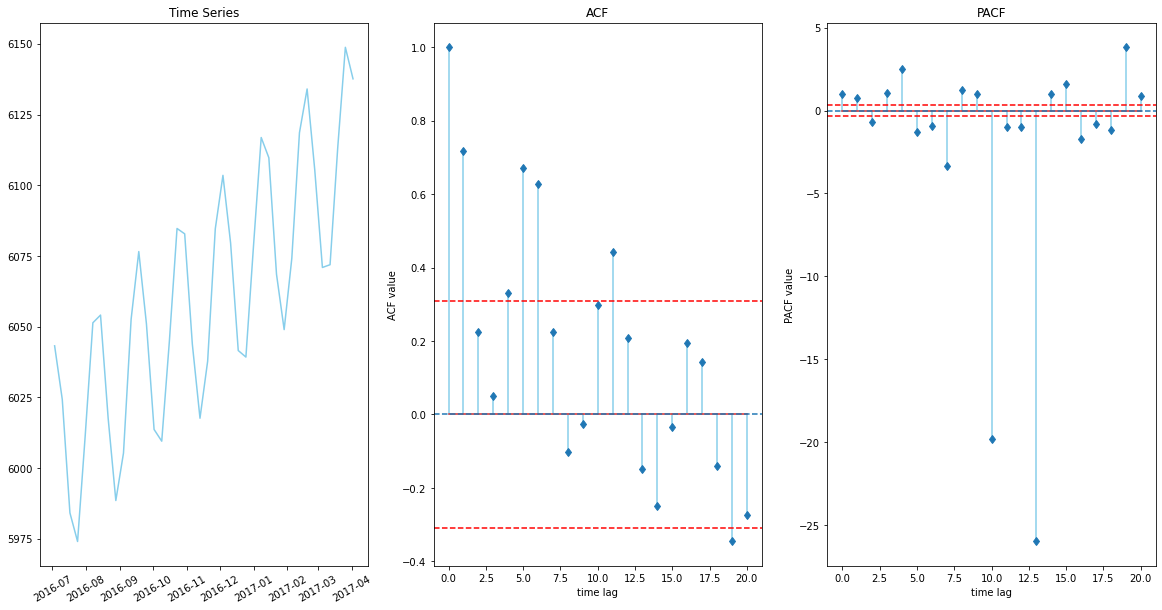
\includegraphics[width=1\textwidth]{SectionLetsMath/elemStat_figures/fig_ACFPACF.png}
\captionsetup{type=figure}
\caption{An example of the ACF and PACF of a time series.}
\label{fig_ACFPACF}
\end{figure}

\subsection{Distance between random variables}
In many applications, it is interesting to have a measure of the distance between two random variables as, for example, the distance between two points on a line, chosen with a law of probability. \par

The distance function is a random variable $Z$ estimated as $Z=|x-y|$. We need to estimate its PDF or CDF to get knowledge about $Z$. By the definition of $F$ we have:

\begin{equation}
F_z\left(z\right)=Prob{\left\{Z\le z\right\}}=Prob\left\{\left|x-y\right|\le z\right\}
\label{eq_Distance1}
\end{equation}

It is necessary to integrate the density function $f_Z$ in the domains $D_X$, and $D_Y$, to calculate $F_Z$.In order to define the domains $D_X$ and $D_Y$, it is necessary to consider the function $Z=\left|X-Y\right|$ on the plan x,y (see Figure \ref{fig_DistanceDomain}).

% INSERT fig_DistanceDomain
\begin{figure}[hbt!]
\centering
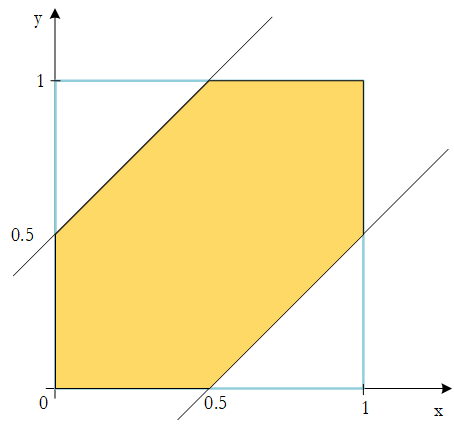
\includegraphics[width=0.7\textwidth]{SectionLetsMath/elemStat_figures/fig_DistanceDomain.png}
\captionsetup{type=figure}
\caption{Domain of the random variable $Z=|X-Y|$}
\label{fig_DistanceDomain}
\end{figure}

The value of $F_Z$ can be determined from the PDF $f_{XY}$.

\begin{equation}
F_z\left(z\right)=\int_{D_X}\int_{D_Y}{f_{xy}\left(x,y\right)dxdy}
\label{eq_Distance2}
\end{equation}

Let assume $X$ and $Y$ being independent\footnote{With the independence hypothesis, $f_{XY}=f_X\bullet f_Y$} and uniformly distributed on $[0,p]$. 

\begin{equation}
    \label{eq_Distance3}
    \begin{split}
    X~U\left[0,p\right];f_x=\frac{1}{p};F_x=\frac{x}{p} \\
    Y~U\left[0,p\right];f_x=\frac{1}{p};F_x=\frac{y}{p} \\
    \end{split}
\end{equation}

The value of $F_Z$ is consequently defined as:

\begin{equation}
F_Z(z)=\int_{D_X}\int_{D_Y}{f_x\left(x\right)f_y(y)dxdy}
\label{eq_Distance4}
\end{equation}

The domain of the function is one out of the three regions of plan defined by the corresponding equalities $Y=X+Z$ , $Y=X-Z$. In Figure \ref{fig_DistanceDomain}, $Z=0.5$. The region is the one between the two lines. It is, then possible to obtain $F_Z$. 
\begin{center}
\begin{equation}
    \label{eq_Distance5}
    \begin{split}
    F_z\left(z\right) =\int_{x=0}^{x=p-z}{\int_{y=0}^{y=z+x}{\frac{1}{p}\times\frac{1}{p}dy\ dx\ }}  + \int_{x=p-z}^{x=z}\int_{y=0}^{y=p}{\frac{1}{p}\times\frac{1}{p}dy\ dx\ }+ \\
    +\ \int_{x=z}^{x=p}{\int_{y=x-z}^{y=p}{\frac{1}{p}\times\frac{1}{p}dy\ dx\ }=} \\
    =\frac{1}{p^2}\left\{\int_{x=0}^{x=p-y}\left(x+z\right)dx+\ \int_{x=p-z}^{x=z}pdx+\ \int_{x=z}^{x=p}\left(p-x+z\right)dx\right\} \\
    =\frac{z\left(2p-z\right)}{p^2} \\
    \end{split}
\end{equation}
\end{center}


The PDF $f_Z$ is defined from equation \ref{eq_cdfIntegralPdf} as follows.

\begin{equation}
f_Z(z)=\frac{dF(z)}{dz}=\frac{2\left(p-z\right)}{p^2}
\label{eq_Distance6}
\end{equation}

We can test that $f_z$ is a PDF since by the definition of $X$,$Y$ its domain is $[0,p]$ and its integral equals 1.

\begin{equation}
f_{Z\left(z\right)}=\int_{0}^{p}\frac{2\left(p-z\right)}{p^2}dz=\left[\frac{2z^2}{2p^2}\right]_0^p=1\ \ 
\label{eq_Distance7}
\end{equation}

At this stage, all the properties of $Z$ are defined by $f$ and $F$. For example, it is possible to calculate the mean value corresponding to the average distance between $X$ and $Y$. 

\begin{equation}
    \label{eq_Distance8}
    \begin{split}
    E\left[Z\right] & =\int_{0}^{p}\frac{2\left(p-z\right)}{p^2}zdz=\frac{1}{p^2}\int_{0}^{p}\left(2pz-{2z}^2\right)dz= \\
    & =\frac{1}{p^2}\left[\frac{2pz^2}{2}-\frac{{2z}^3}{3}\right]_0^p=\frac{1}{p^2}\left[p^3-\frac{2p^3}{3}\right]= \\
    & = \frac{p}{3} \\
    \end{split}
\end{equation}
The procedure above can be applied to any probability distribution of $X$ and $Y$ under the independence hypothesis.

\section{Statistics} \label{secStatistics}

The statistic is an application of the probability theory to infer the properties of a population of elements working on a small subset of it (i.e. a sample). The statistic was born to solve the trade-off between the time necessary to collect data on-field and the accuracy of the information obtained by these data. In fact, it is always impossible to collect all the information available since the population counts thousand or millions of different elements. Statistics provides models to get robust results even when we have few observations of a physical phenomenon.

\subsection{Estimators} \label{secEstimators}

Statistics usually follows a precise workflow:
\begin{enumerate}
    \item Collect data; 
    \item Sample data;
    \item Infer properties from samples to the whole population.
\end{enumerate}

The last step is the one we are interested in the most: we need to estimate the parameters of the probability distribution of the population. Estimators are used to calculating the value of a parameter of a population (e.g., the mean or the variance) based on the observed values given by the sample. Estimators are classified as biased or unbiased. We call an estimator $\hat{\theta}$ of a parameter $\theta$ unbiased when $E\left[\hat{\theta}\right]=\theta$.\par

The most common estimators are needed for the estimation of $\mu\ $ and $\sigma $ of the population. The sample mean $\bar{X}$ is an unbiased estimator of $\mu$ (see equation \ref{eq_sampleMean}). While the sample variance $S^2$ is an unbiased estimator for $\sigma^2$ (see equation \ref{eq_sampleVariance}).

\begin{equation}
\bar{X}=\frac{X_1+\ldots+X_N}{N}
\label{eq_sampleMean}
\end{equation}

\begin{equation}
S^2=\frac{1}{N-1}{\sum_{i}^{N}\left(X_i-\bar{X}\right)^2}
\label{eq_sampleVariance}
\end{equation}

Estimators are evaluated according to their accuracy (i.e. their closeness to the random variable they estimate). In general, we can find two sources of inaccuracy on an estimator: the bias and the variance. Let assume having a model f producing an estimator $\hat{\theta}$ for the random variable $\theta$ with an error $\epsilon$. 

\begin{equation}
\theta \simeq \hat{\theta}=f\left(X\right)+\epsilon
\label{eq_bias1}
\end{equation}
A vector $x_0$ defines a set of realisations of $X$ and we want to define the error of the estimator $\hat{\theta}$.

\begin{equation}
    \label{eq_bias2}
    \begin{split}
    \epsilon\left(x_0\right) = E\left[\left(\hat{\theta}-\hat{f}\left(X\right)\right)^2|X=x_0\right]= \\
     =\ E\left[\left(\hat{\theta}-E\left[\hat{f}\left(x_0\right)\right]+E\left[\hat{f}\left(x_0\right)\right]-\hat{f}\left(x_o\right)\right)^2\right]=\\
     = E[\left(\hat{\theta}-E\left[\hat{f}\left(x_0\right)\right]\right)^2 + \left(E\left[\hat{f}\left(x_0\right)\right]-\hat{f}\left(x_o\right)\right)^2 + \\ 2\left(\hat{\theta}-E\left[\hat{f}\left(x_0\right)\right]\right)\times \left(E\left[\hat{f}\left(x_0\right)-\hat{f}(x_0)\right]\right)]=\\
     =E\left[\left(\hat{\theta}-E\left[\hat{f}\left(x_0\right)\right]\right)^2\right] +E\left[\left(E\left[\hat{f}\left(x_0\right)\right]-\hat{f}\left(x_o\right)\right)^2\right] + \\
     + E\left[2\left(\hat{\theta}-E\left[\hat{f}\left(x_0\right)\right]\right)\left(E\left[\hat{f}\left(x_0\right)-\hat{f}\left(x_0\right)\right]\right)\right]=\\
     Var\left(\hat{f}\left(x_0\right)\right)+\left(E\left[\hat{f}\left(x_0\right)\right]-\hat{f}\left(x_o\right)\right)^2\\
     =Var\left(\hat{f}\left(x_0\right)\right)+\ Bias^2\left(\hat{f}\left(x_0\right)\right)\\
    \end{split}
\end{equation}


The error of an estimator can be defined according to \ref{eq_bias2} using:
\begin{itemize}
    \item 	$Bias^2\left(\hat{f}\left(x_0\right)\right)$ is the squared bias in the estimation of the mean. It describes how much the mean of the estimator is far from the true mean.
    \item 	$Var\left(\hat{f}\left(x_0\right)\right)$ is the deviation of the estimator around its mean.
\end{itemize}

The role of the variance and bias can be easily visually interpreted in Figure \ref{fig_biasVariance}.

% INSERT fig_biasVariance
\begin{figure}[hbt!]
\centering
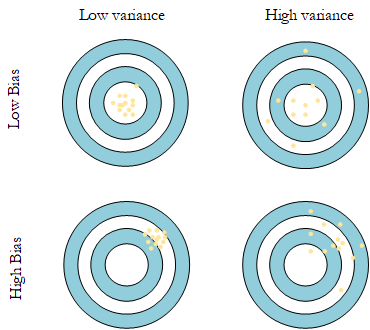
\includegraphics[width=0.7\textwidth]{SectionLetsMath/elemStat_figures/fig_biasVariance.png}
\captionsetup{type=figure}
\caption{The bias and variance of an estimator}
\label{fig_biasVariance}
\end{figure}

Complex prediction models developed using data-driven methods, have to take into account the variance and the bias of the predictions they produce. In particular, there is a bias-variance trade-off. Typically, the more complex the model, the lowest the variance and the highest the bias produced by predictions of the models. On the opposite, a simple model leads to low bias but high variance. Practically speaking, it is always necessary to take into account the bias and the variance of the response of a model to check if it fits with its purpose. Developing a complex model to solve a simple problem is just a way to add additional variance to the responses of the model. In general, we keep a model as simpler as possible (according to the Ockham's razor principle). \par

We introduce the Gauss-Markov theorem to show an important property of the linear regression estimator (see chapter \ref{chapLinearRegression}). Let $\hat{\theta}=c^Ty$ be an unbiased estimator of:

\begin{equation}
\alpha^T\beta=\alpha^T\left(X^TX\right)^{-1}X^Ty
\label{eq_biasLinearRegression1}
\end{equation}

Then:

\begin{equation}
E\left[c^Ty\ \right]=\alpha^T\beta
\label{eq_biasLinearRegression2}
\end{equation}

\begin{equation}
Var\left(\alpha^T\hat{\beta}\right)\le Var(c^Ty\ )
\label{eq_biasLinearRegression3}
\end{equation}

The \ref{eq_biasLinearRegression1} is the expression of a linear regression of $\theta=\alpha^T\beta$. In other words, a linear regression  provides the lowest variance estimator possible. The lowest variance does not imply a lower error in the prediction since we have no information about the other error component (i.e. the bias). Nevertheless, we should prefer linear regression, that is a very simple model, when we are sure there is no bias, i.e. $E\left[E\left[\hat{\theta}\right]-\theta\right]^2=0$. In other words, when the world behaves linearly, use a linear model.

\subsection{Maximum Likelihood Inference}
In many practical cases, we need to get a good estimate of a parameter $\theta$ of a PDF, given a sample of the population. Maximum likelihood estimation (MLE) is the tool to do that. We define a function $g_\theta(z)$; where $g$ is the PDF (e.g., normal distribution) of $z_i$ and $\theta$ are the unknown parameters to estimate (e.g. the mean and the variance $\mu$, $\sigma^2$). We need to find values of $\theta$ such that they properly represent the statistical sample. This equals to imply the maximisation of a likelihood function $L$.

\begin{equation}
L\left(\theta,\ Z\right)=\prod_{i=1}^{N}{g_\theta(z_i)}
\label{eq_MLE1}
\end{equation}

The maximisation is done by considering the logarithm of $L$. Maximising $L$ will maximise $\log(L)$ too, due to the monotony of the logarithm. To get a maximum likelihood estimation, we need to maximise:

\begin{equation}
l\left(\theta,Z\right)=\sum_{i=1}^{N}{l\left(\theta,z_i\right)=\sum_{i=1}^{N}\log{\left(g_\theta\left(z_i\right)\right)}}
\label{eq_MLE2}
\end{equation}

This is done by looking for $\theta$ maximising the function:

\begin{equation}
\dot{l}\left(\theta,Z\right)=\ \sum_{i=1}^{N}{\dot{l}\left(\theta,z_i\right)=\sum_{i=1}^{N}{\frac{\partial l\left(\theta,z_i\right)}{\partial\theta}=0}}
\label{eq_MLE3}
\end{equation}
In practical cases, it may be difficult to express the formula of the PDF $g$ and to calculate its derivative to get an MLE. Computerised algorithms have been implemented to solve this problem by approximation where it is not possible to solve it analytically. Bootstrap and Montecarlo simulation are common examples.

\subsection{Kernel Density Estimation} \label{secKernelDensityEstimation}
The estimation of a PDF, can be obtained using a graphic methodology, instead of mathematically define its parameters. Having a set of empirical observations, it is always possible to use a histogram to represent its frequency analysis. The width of each bin of the histogram defines the shape of the curve. Figure \ref{fig_empiricalBinning} shows different histograms of the same empirical sample by using different widths of the histogram bins.\footnote{The source code of Figure \ref{fig_empiricalBinning} is available \href{https://github.com/aletuf93/logproj/blob/master/examples/03.\%20Statistics.ipynb}{here}.
}

% INSERT fig_empiricalBinning
\begin{figure}[hbt!]
\centering
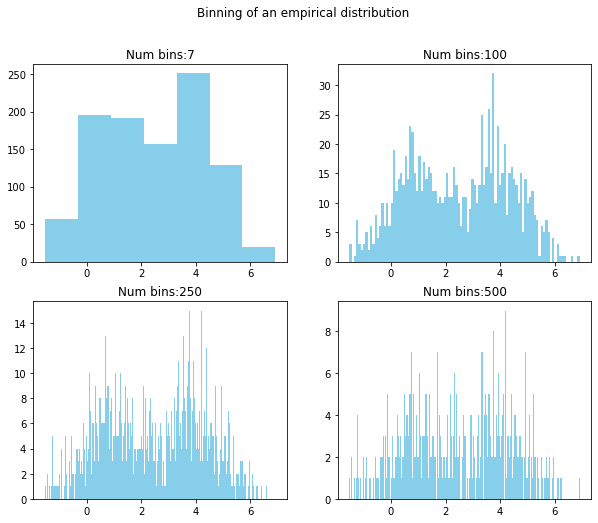
\includegraphics[width=0.7\textwidth]{SectionLetsMath/elemStat_figures/fig_empiricalBinning.png}
\captionsetup{type=figure}
\caption{Definition of histograms with different bin size}
\label{fig_empiricalBinning}
\end{figure}

Kernel Density Estimation (KDE) is a procedure to estimate the PDF of a random variable based on its observations. The idea is to define the shape of the PDF based on the empirical values smoothed around a local region $b$ called bandwidth. This is similar to the choice of the number of bins to define a histogram. KDE can be expressed as:

\begin{equation}
\hat{f}=\frac{1}{n}\sum_{i}^{n}K\left(\frac{x-x(i)}{b}\right)
\label{eq_KDE}
\end{equation}

Where K is a kernel function with a peak on 0 (it is common to use a gaussian function). Figure \ref{fig_KDE} shows the effect of different KDEs with several values of b. \footnote{The source code of Figure \ref{fig_KDE} is available \href{https://github.com/aletuf93/logproj/blob/master/examples/03.\%20Statistics.ipynb}{here}.}

% INSERT fig_KDE
\begin{figure}[hbt!]
\centering
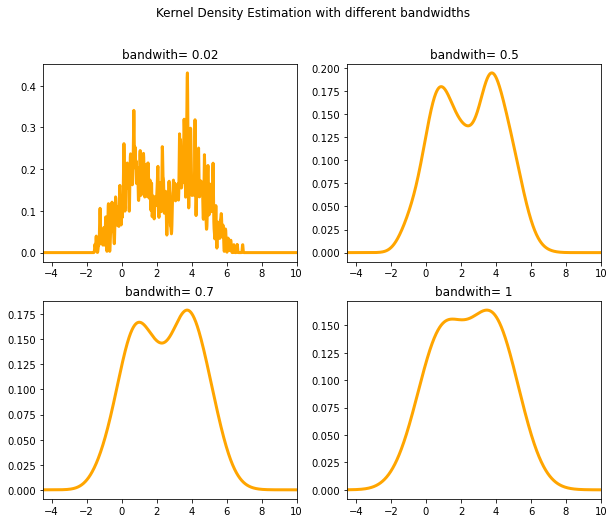
\includegraphics[width=0.7\textwidth]{SectionLetsMath/elemStat_figures/fig_KDE.png}
\captionsetup{type=figure}
\caption{KDE with different bandwidths to estimate the PDF of an empirical sample.}
\label{fig_KDE}
\end{figure}

\subsection{Bootstrapping method} \label{secBootstrapping}

Bootstrapping is an algorithm used to estimate the value of a parameter $\alpha$ (e.g. the mean or variance) from a population where its PDF is unknown or too difficult to estimate analytically.  Let X be a set of observations with cardinality $n$. Algorithm \ref{algo_bootstrap} illustrates the Bootstrapping method.

\begin{algorithm}[H]
\DontPrintSemicolon
\SetAlgoLined
Set the number of iterations B\;
\For{$i=1:B$}{
    Set $\beta$ = $n$ points randomly picked from $X$. \;
    Use $\beta$ to estimate the parameter $\alpha$. \;
}
Define the confidence interval of $\alpha$ using the statistic of the $B$ iterations; $\bar{\alpha}=\frac{1}{B}\sum_{i=1}^{B}\alpha_i$ \;
\caption{Bootstrapping algorithm}
\label{algo_bootstrap}
\end{algorithm}

\subsection{Montecarlo method} \label{secMontecarlo}
Montecarlo simulation is a valid alternative to measure the outcome of a process where many random variables with given PDF are involved, but their joint distribution is hard to compute. \par

Let consider the random variables $X_i$ $i=1,\ldots,q$ whose distribution are given and $\alpha=f(X_i)$. We need to infer properties on the distribution of $\alpha$. Algorithm \ref{algo_montecarlo} shows the Montecarlo simulation to estimate the distribution of $\alpha$. 

\begin{algorithm}[H]
\DontPrintSemicolon
\SetAlgoLined
Set the number of iterations M\;
\For{$i=1:M$}{
    Sample the value for each $X_i$, $i\in q$ according to their PDFs \;
    Evaluate $\alpha=f(X_i)$  \;
}
Define the confidence interval of $\alpha$ using the statistic of the $M$ iterations; $\bar{\alpha}=\frac{1}{M}\sum_{i=1}^{M}\alpha_i$ \;
\caption{Montecarlo algorithm}
\label{algo_montecarlo}
\end{algorithm}

\subsection{Data collection and Measurement systems} \label{secMeasurementSystem}
Dealing with empirical data, it is always necessary to define a measurement system to pick accurate data on-field. If the measurement system is not accurate or not precise, all the following analyses will keep an underlying error. A measurement system determines the measured value $X_1$ of a realisation $X_{true}$. Having:

\begin{equation}
X_1=X_{true}+\beta+\epsilon
\label{eq_measurement1}
\end{equation}

Where $X_{true}$ is the real value of the variable; $\beta$ is the bias (accuracy or systematic error), i.e. how much far the (average value) of the measure from $X_{true}$; $\epsilon$ are random errors depending on the precision of the measurement system. A good measurement procedure has:

\begin{equation}
\mu=\lim_{N \to +\infty}{\frac{1}{N}\sum_{i=1}^{N}{X_i=X_{true}+\beta}}
\label{eq_measurement2}
\end{equation}

\begin{equation}
\lim_{N \to +\infty}{\frac{1}{N}\sum_{i=1}^{N}{\epsilon_i=0}}
\label{eq_measurement3}
\end{equation}

The analysis of uncertainty aims at the definition of $\beta$ and $\epsilon$ of data collected on-field, providing methods to handle and process empirical data correctly.

\subsubsection{Systematic errors}
Systematic error (or bias errors) is determined by a measure of the accuracy of the measurement instrument. Systematic errors occur when an instrument has not an appropriate level of accuracy compared to the variable one wants to measure. For example, it is inadequate to measure the length of a warehouse rack using a ruler. A measurement instrument always requires calibration to be accurate. For example, using a calliper, the systematic error is often linked to a wrong calibration. 

\subsubsection{Uncertainty errors}
Uncertainty error (or random errors) is a measure of precision linked with the random nature of the measurement process. This is unavoidable and must be normally distributed in any empirical data collection (e.g., the processing time of a part on a workbench should be normally distributed when the process is under control).

\subsubsection{Mistakes}
Mistakes are data points with wrong values. They may be error storing the results of an experiment or outliers which must be deleted when there are solid arguments against the value of these data points.

\subsubsection{Data cleaning}
The process of cleaning data implies deleting data points whose value is outside the limit of the analysis one wants to perform. In particular, it often happens to have outliers whose measure is due to errors, having no connection with the real measure. We introduce two methodologies to deal with outliers.\par

The Chauvenet’s criterion provides a simple method to deal with outliers assuming that data have a Gaussian distribution with mean $\mu$ and standard deviation $\sigma$. Let consider a point $i$ with value $x_i$ to be suspect of being an outlier. Its $t$-value is defined as $t_i=\frac{|x_i-\mu|}{\sigma}$. Chauvenets’ criterion considers the probability that $i$ is found inside or outside a probability band defined as $P=1-\frac{1}{2N}$; where $N$ is the number of samples. Chauvenet’s criterion defines $z=Prob\left(t_i\sigma\notin P\right)\times N$. If $z<0.5$ the point should be rejected. In other words, if a point $i$ is too far from the mean of the normal distribution associated with the sample, it should be rejected. \footnote{The source code of the Chauvenet's method is available \href{https://github.com/aletuf93/logproj/blob/master/logproj/ml_dataCleaning.py}{here}.
} \par
The second methodology we introduce to deal with outliers is the interquartile range (IQR). The IQR method considers the range between the $25^{th}$ and the $75^{th}$ percentile of the data points to detect outliers. In particular, being $IQR = Q_3 - Q_1$, where $Q_1$, and $Q_3$ are the first and the third quartile (equivalent to the $25^{th}$, and the $75^{th}$ percentiles), outliers are found below $Q_1 - (1.5\times IQR)$, and above $Q_3 + (1.5\times IQR)$.\footnote{The source code of the IQR method is available \href{https://github.com/aletuf93/logproj/blob/master/logproj/ml_dataCleaning.py}{here}.
}


\section{Statistical Distributions}
This section introduces the relevant statistical distribution for the applications in the field of logistics and operations.

\subsection{The Normal distribution}
The most important probability distribution is called normal (or Gaussian) distribution, and its PDF is defined as:

\begin{equation}
f\left(X\right)=\frac{e^{-\frac{(X-{\mu)}^2}{2\sigma^2}}}{\sigma\sqrt{\left(2\pi\right)}}
\label{eq_pdfGaussian}
\end{equation}

Having mean $\mu=\sum_{i=1}^{N}\frac{x_i}{N}$, and standard deviation $\sigma=\left[\frac{1}{N}\sum_{i}^{N}\left(X_i-\mu\right)^2\right]^\frac{1}{2}$. When the distribution has a large standard deviation, its peak tends to be lower.\par
The Normal distribution is characterized by a concentration of the observation around the mean. It is possible to control the density of the function with reference to the distance from the mean $\mu$ expressed in terms of the number of standard deviations $\sigma$ (Figure \ref{fig_normal}).

% INSERT fig_normal
\begin{figure}[hbt!]
\centering
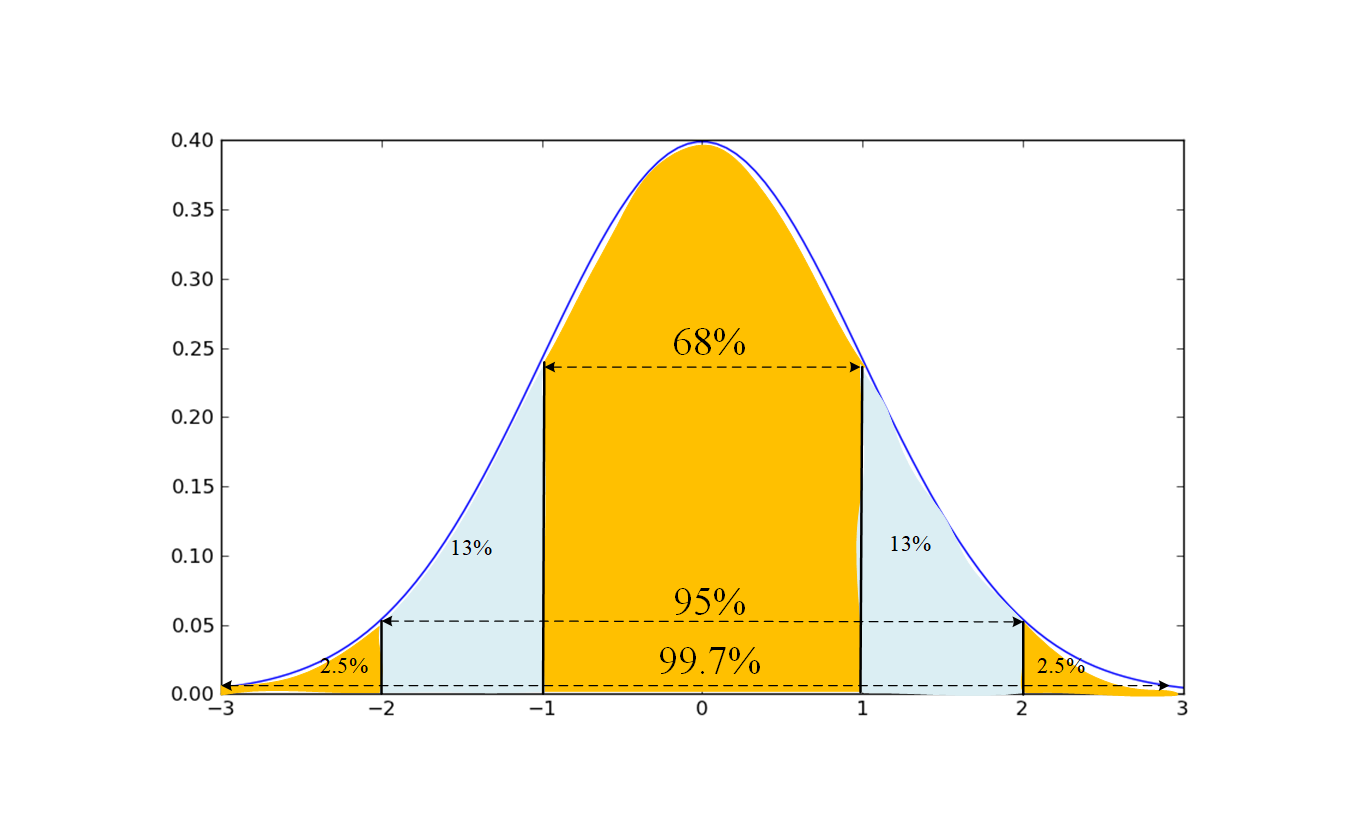
\includegraphics[width=0.9\textwidth]{SectionLetsMath/elemStat_figures/fig_normal.png}
\captionsetup{type=figure}
\caption{Normal distribution probability distribution function (PDF).}
\label{fig_normal}
\end{figure}

When a random variable $X$ is normally distributed, we can prove that there is a  probability equal to $0.95$ that its mean value is found within a confidence interval of $1.96\sigma$.

\begin{equation}
Prob\left\{-1.96\le\frac{X_i-\mu}{\sigma}\le1.96\right\}=0.95
\label{eq_pdfConfidenceInterval1}
\end{equation}

\begin{equation}
Prob\left\{X_i-1.96\sigma\le\mu\le X_i+1.96\sigma\right\}=0.95
\label{eq_pdfConfidenceInterval2}
\end{equation}

A normal distribution has many useful properties. In practice, it is necessary to prove that a sample is normally distributed (e.g. using statistical tests see \ref{secStatTest}) to apply all the magical properties of the normal distribution. This way, by estimating the $\sigma$ of the populations using the estimator $s=\frac{1}{N-1}\sum_{i=1}^{N}{{{(X}_i-\bar{X})}^2\ \ }$, the mean value $\mu$ of the population will have a confidence interval of 95\% within the range $\pm1.96\sigma$. The central limit theorem generalises these properties of the normal distribution to any statistical distribution.

\subsection{Central limit theorem}
The central limit theorem states that describing an event with a sufficiently large number $N$ (with $N\geq30$) of random variables $X_i$, the arithmetic mean of these variables is normally distributed.

\begin{equation}
\bar{x}=\frac{X_1+X_2+\ldots+X_N}{N} \sim N(\mu,\sigma)
\label{eq_centralLimitTheorem}
\end{equation}



In other words, no matter the distribution of the random variables $X_i$, increasing the number of experiments measuring $X_i$, there is a random variable describing the mean value of the experiments, and it is normally distributed.

\subsection{Multivariate normal distribution}
The multivariate normal distribution generalizes the univariate normal distribution to a multidimensional space. Assume $X=\left(X_1,\ldots,X_p\right)^T$ be a $p$-dimensional random vector. $X$ is distributed as a multivariate normal distribution when its density function is as follows.

\begin{equation}
X\sim N_p\left(\mu,\Sigma\right)= f\left(x_1,\ldots,x_p\right)=\frac{1}{\left(2\pi\right)^\frac{p}{2}\left|\Sigma\right|^\frac{1}{2}}e^{-\ \frac{1}{2}\left(x-\mu\right)^T\Sigma^{-1}(x-\mu)}
\label{eq_multivariateNormal}
\end{equation}

Where $\mu$ is the mean vector $\mu=E\left[X\right]=\left[E\left[X_1\right],E\left[X_2\right],\ldots,E\left[X_p\right]\right]^T$ and $\Sigma$ is a $p\times p$ covariance matrix $\Sigma_{i,j}=E\left[\left(X_i-\mu_i\right)\left(X_j-\mu_j\right)\right]=Cov[X_i,X_j]$.

\subsection{The Poisson Distribution} \label{secPoisson}
The Poisson distribution is a discrete probability distribution useful to describe the realisations of events when the average time between the event is given, but the interarrival time between the events is random. This situation is common when dealing with queues (the average throughput of the resource is given, but the interarrival time of the workload is random) or maintenance (the mean time to failure is given, but the exact failure time is unknown). The Poisson distribution has PDF:

\begin{equation}
Prob\left(X=k\right)=\frac{\lambda^ke^{-\lambda}}{k!}
\label{eq_poissonPDF}
\end{equation}

The Poisson distribution identifies the probability of realisation of $k$ events within a time interval $\tau$ having an average number of event per time unit $d$, where $\lambda=d\tau$. Figure \ref{fig_poisson} identifies the shape of the PDF of the Poisson distribution using different values of $\lambda$.\footnote{The source code of Figure \ref{fig_poisson} is available \href{https://github.com/aletuf93/logproj/blob/master/examples/03.\%20Statistics.ipynb}{here}.
}


% INSERT fig_poisson
\begin{figure}[hbt!]
\centering
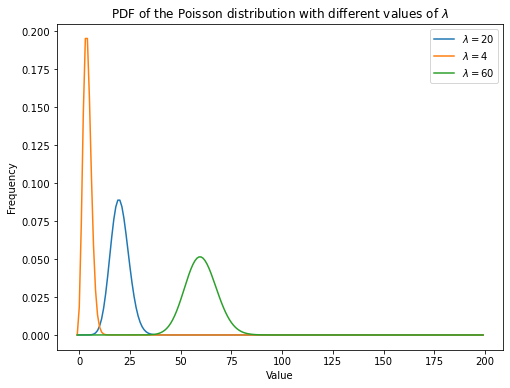
\includegraphics[width=0.9\textwidth]{SectionLetsMath/elemStat_figures/fig_poisson.png}
\captionsetup{type=figure}
\caption{Poisson distribution probability distribution function (PDF).}
\label{fig_poisson}
\end{figure}

\subsection{The Triangular Distribution}
Some times empirical measurements are done on the minimum, maximum and average value of a random variable $X$. In these situations, we have only three values to infer the properties of the random variable $X$. Triangular distribution assumes $X$ having a density with a triangular shape with its mode in correspondence of the mean value, and the vertices at the minimum and maximum values. The triangular distribution has PDF:

\begin{equation}
f(X)=\left\{
                \begin{array}{ll}
                  0\ \ & if\ X<a,\\
                  \frac{2(X-a)}{(b-a)(c-a)}\ & if\ a\le X\le c,\\
                  \frac{2}{b-a}\ & if\ X=c,\\
                  \frac{2(b-X)}{(b-a)(b-c)}\ & if\ c<X\le b,\\
                  0\ & if\ b<X
                \end{array}
              \right.
\label{eq_triangularDF}
\end{equation}

Where $a$ is the minimum value, $b$ is the maximum value, and $c$ is the mean value. Figure \ref{fig_triangular} shows the shape of a triangular distribution.\footnote{The source code of Figure \ref{fig_triangular} is available \href{https://github.com/aletuf93/logproj/blob/master/examples/03.\%20Statistics.ipynb}{here}.
}

% INSERT fig_triangular
\begin{figure}[hbt!]
\centering
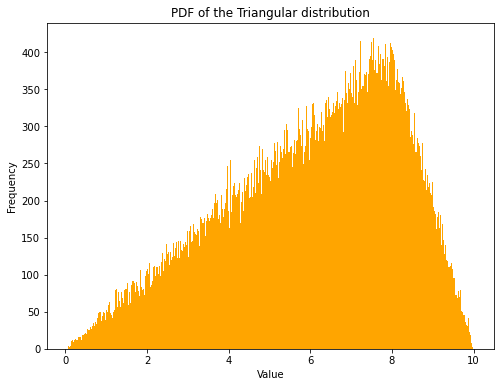
\includegraphics[width=0.9\textwidth]{SectionLetsMath/elemStat_figures/fig_triangular.png}
\captionsetup{type=figure}
\caption{Triangular distribution probability distribution function (PDF).}
\label{fig_triangular}
\end{figure}

\section{Statistical tests} \label{secStatTest}

All the statistical tools introduced so far have been used with a descriptive purpose, i.e. to describe the behaviour of an experiment. At some point, it may be necessary to use statistical tools to get answers about the validity of a theory (e.g. a research intuition). Statistical tests are used for this reason. A statistical test checks if a “test distribution” (e.g., Gaussian, $t$, $\chi^2$) fits with the empirical data. The workflow of a statistical test is as follows.
\begin{enumerate}
    \item Identify the problem and the parameters of interests;
    \item State the null hypothesis $H_0$;
    \item State the alternative hypothesis $H_1$;
    \item Identify a level of significance $\alpha$;
    \item Choose an appropriate statistical test;
    \item Define the rejection region for the null hypothesis;
    \item Compute the test and check whether $H_0$ should be rejected or not.
\end{enumerate}

$H_0$ (or, more often $H_1$) is the hypothesis (e.g. the research intuition one wants to test). Engineeringly speaking, $H_0$ is often formulated as the opposite of what one wants to test. Such that, rejecting $H_0$ is a successful test since it supports the initial thesis.\par

A typical null hypothesis is that there are no differences between two parameters (e.g., the means $\mu_1$ and $\mu_2$) observed from two populations (i.e. they have the same distribution and the differences between them are only due to the chance). The hypothesis is tested within a certain level of significance $\alpha$. Any statistical test works calculating a probability $p$ called $p$-value.\par

The $p$-value is the probability of obtaining an empirical result more extreme than the observed ones due to the sample variability, assuming $H_0$ being true. In other words, the $p$-value is an estimation of the probability that rejecting the null hypothesis is only due to the chance. A high $p$-value may be due to a bad selection of the sample (e.g., too small) while a low $p$-value suggests the significance of the test.\par

For a random variable $X$ with unknown distribution, we observe a value $x$. The calculation of $p$-value is:

\begin{equation}
p=Prob\left\{ X\le x|H_0\right\}
\label{eq_pvalue}
\end{equation}

Figure \ref{fig_StatTest} shows an example where $X$ is an unknown distribution that is tested to have the same mean $\mu$ of the represented normal distribution. The null hypothesis $H_0$ is that \textit{“the empirical data are normally distributed”}. In the figure on the left, the sample with mean value $X$ is too far from the mean of the distribution and the p-value is low; for this reason, $H_0$ is rejected. Otherwise, in the figure on the right, the sample with mean $X$ behaves as the distribution (within the confidence interval of the test $\alpha=0.05$), the $p$-value is higher than $\alpha$, and $H_0$ is not rejected.

% INSERT fig_StatTest
\begin{figure}[hbt!]
\centering
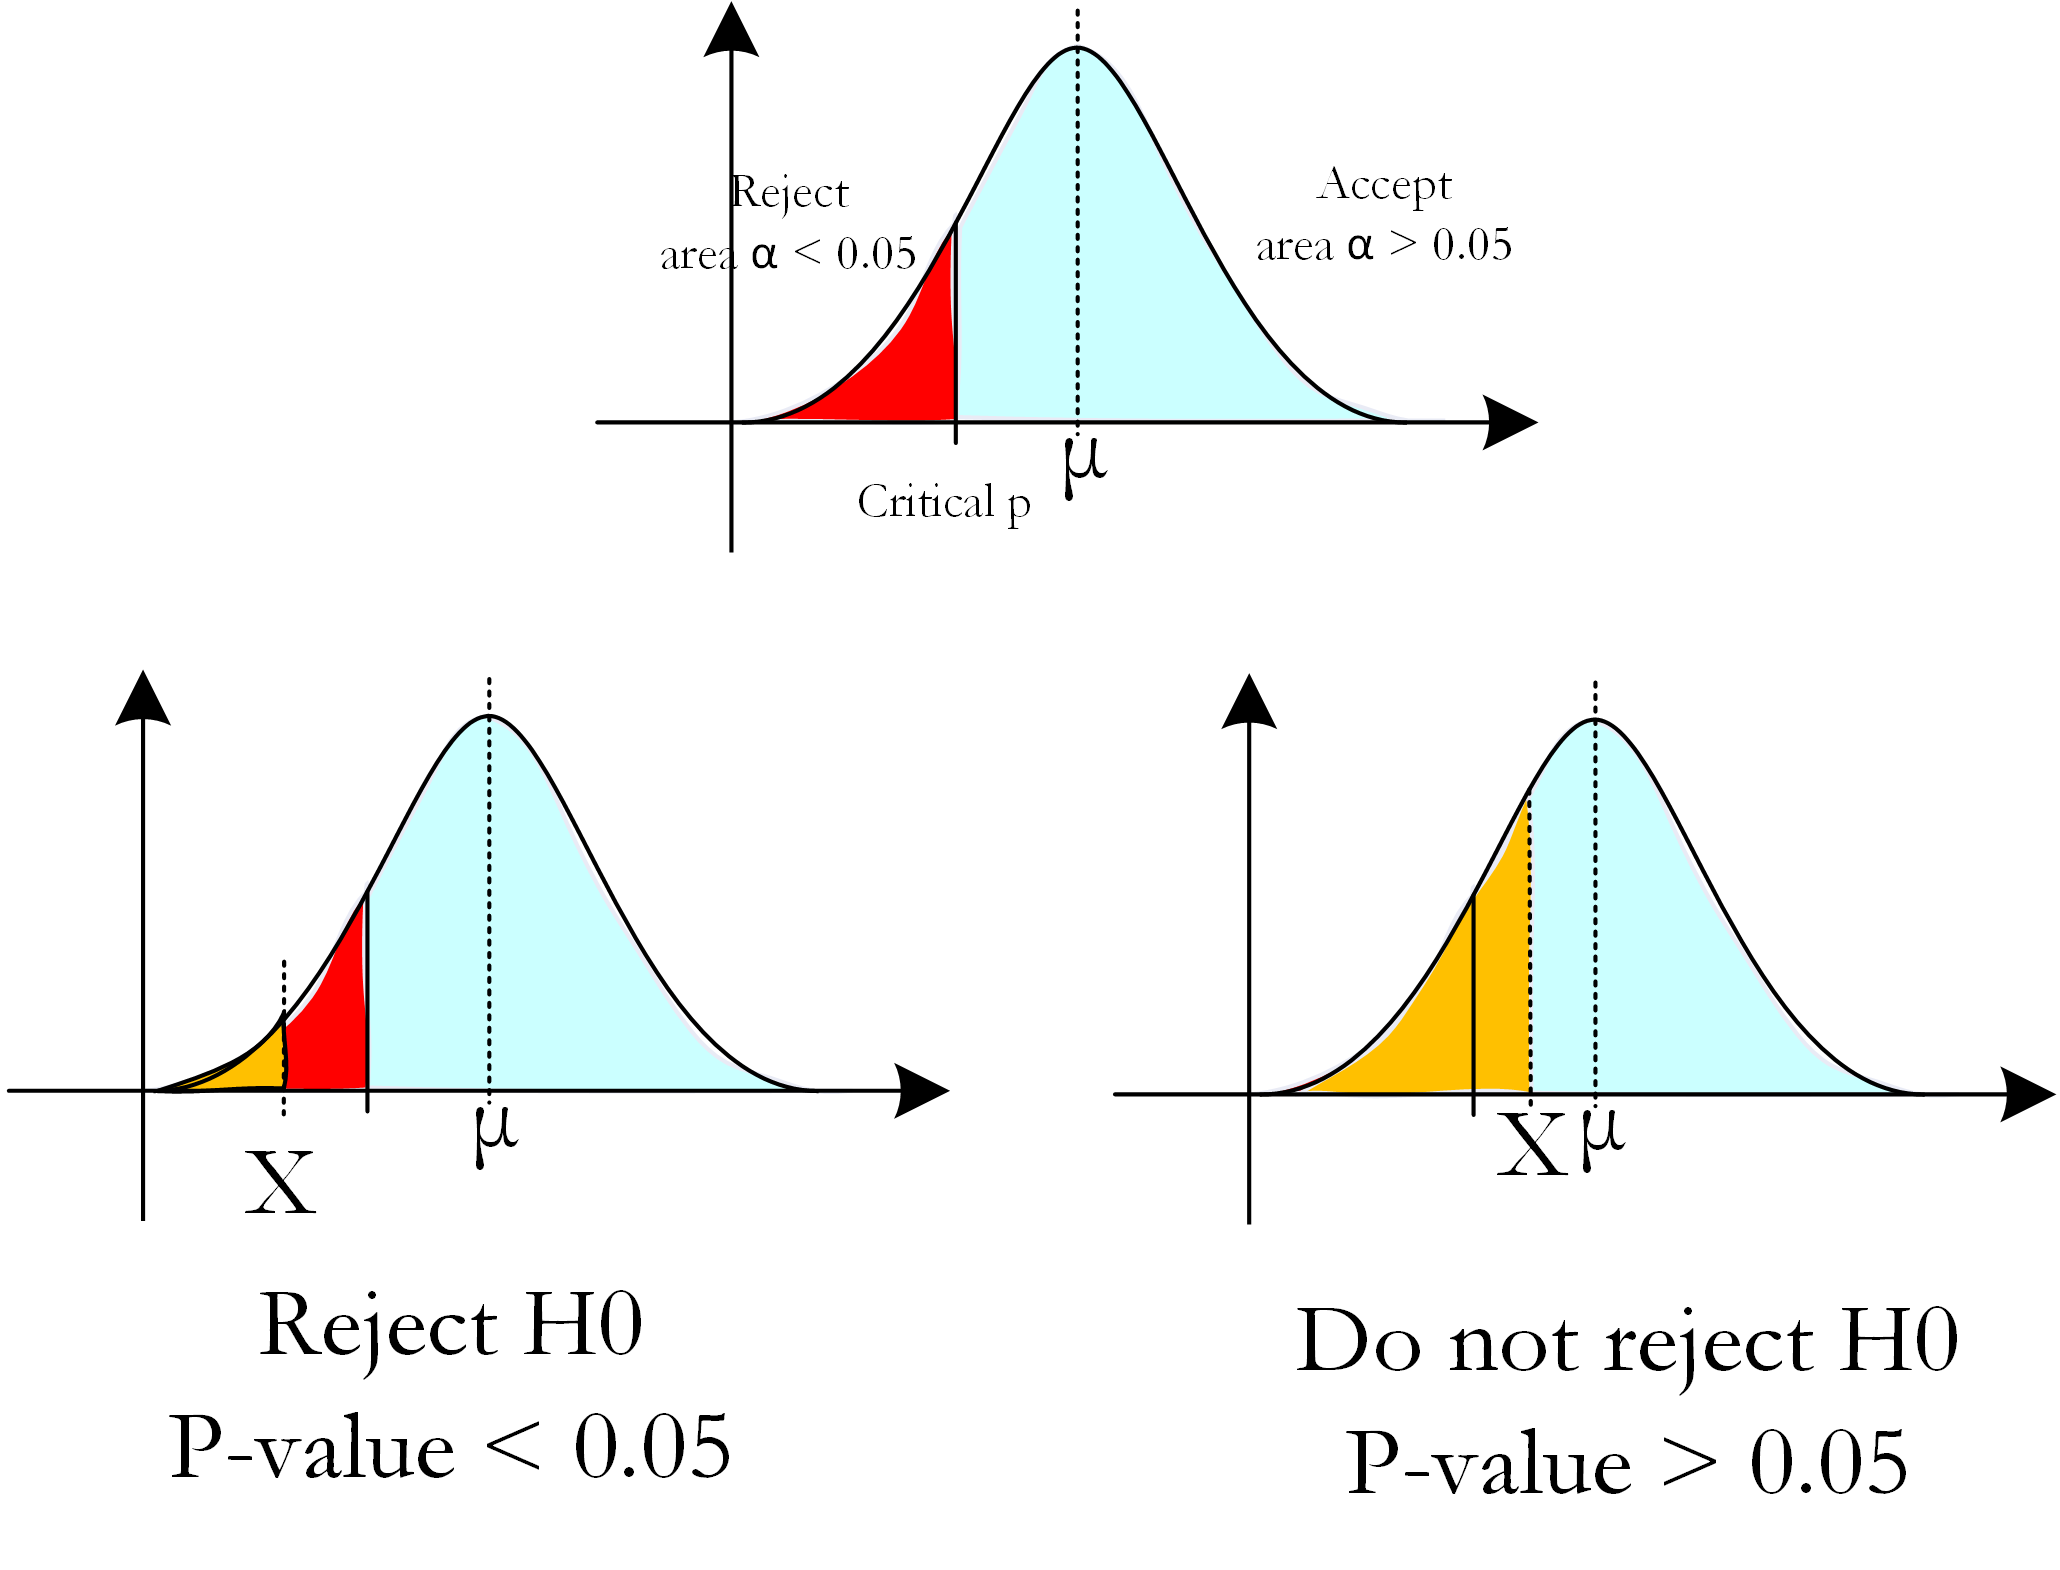
\includegraphics[width=0.9\textwidth]{SectionLetsMath/elemStat_figures/fig_StatTest.png}
\captionsetup{type=figure}
\caption{Graphical representation of a statistical test.}
\label{fig_StatTest}
\end{figure}

The significance of the test depends on the value of $\alpha$ chosen for the test. Table \ref{tab_statTest} shows some common values of $\alpha$ used to accept or discard hypothesis. Please note that $\alpha$ has to be chosen before the test depending on the context and the level of significance expected from the decision-maker. It is a bad practice to make an experiment and afterwards evaluate its results depending on the $p$-value.

% INSERT tab_statTest
\begin{figure}[hbt!]
\centering
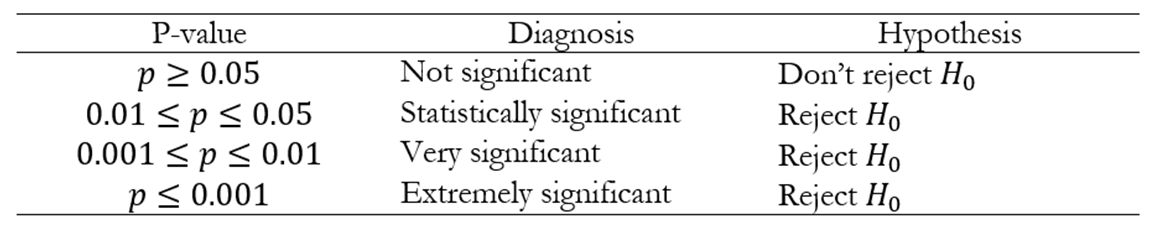
\includegraphics[width=0.9\textwidth]{SectionLetsMath/elemStat_figures/tab_statTest.png}
\captionsetup{type=table}
\caption{$p$-value and levels of significance.}
\label{tab_statTest}
\end{figure}

\subsection{Z-test (normal distribution)}
$Z$-test is used to check if the mean value of a sample is equal to a reference value. In other words, given the value of $\sigma$, one wants to check how far is the sample mean $\bar{X}$ from the population mean $\mu$. Table \ref{tab_zTest} lists the summary of the $Z$-test.


% INSERT tab_zTest
\begin{figure}[hbt!]
\centering
\includegraphics[width=0.9\textwidth]{SectionLetsMath/elemStat_figures/tab_zTest.png}
\captionsetup{type=table}
\caption{Z-test summary.}
\label{tab_zTest}
\end{figure}

$Z$-test assumes a normal distribution and evaluates the $Z$-score of the distribution. The statistic of the test is as follows.

\begin{equation}
Z=\frac{\bar{X}-\mu}{\sigma/\sqrt n}
\label{eq_ztest}
\end{equation}
where $n$ is the number of samples. If $Z<-1.96\ OR\ Z>1.96$ $H_0$ is rejected. The $p$-value is higher than $0.05$ and the value of $\bar{X}$ is too far from $\mu$. If $-1.96\le Z\le1.96$ $H_0$ is accepted since $\bar{X}$ falls within the acceptance region. When the value of $\sigma$ is unknown, or the sample size is too small ($n<30$), a similar test can be performed using a $t$-test.

\subsection{t-test}
The $t$-test aims at checking if a sample behaves like a normal distribution when the sample size $n$ is small. In other words, dealing with a small sample it is important to check if it is possible to apply normal distribution statistics or if the sample belongs to a different distribution. In practice, it is necessary to compare the sample mean $\bar{X}$ and the population mean $\mu$. Since the population variance is unknown, it is assumed $\sigma^2=s^2$ i.e., the variance of the population equals the variance of the sample. The $t$-student distribution measures the difference between the sample mean and the population mean. The statistic of the test follows this distribution.

\begin{equation}
t=\frac{(\bar{X}-\mu)}{s/\sqrt n}
\label{eq_tTest}
\end{equation}

Where $n$ indicates the number of samples i.e., the degree of freedom of the distribution. Consequently , the $t$-distribution has a different shape for different degrees of freedom (see Figure \ref{fig_tDist}).\footnote{The source code of Figure \ref{fig_tDist} is available \href{https://github.com/aletuf93/logproj/blob/master/examples/03.\%20Statistics.ipynb}{here}.} When the number of samples $n$ (i.e. the degrees of freedom) approaches $30$, the $t$-distribution has the same shape of the normal distribution. Table \ref{tab_tTest} illustrates the summary of this test.

% INSERT fig_tDist
\begin{figure}[hbt!]
\centering
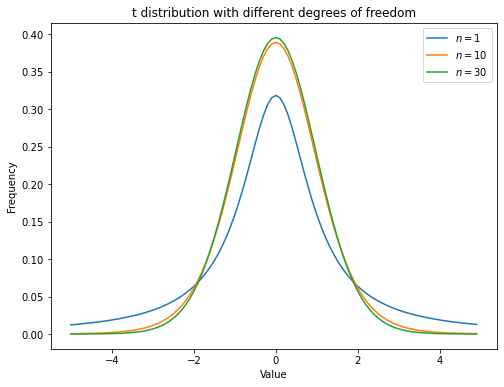
\includegraphics[width=0.9\textwidth]{SectionLetsMath/elemStat_figures/fig_tDist.png}
\captionsetup{type=figure}
\caption{PDF of the $t$-distribution with different degrees of freedom.}
\label{fig_tDist}
\end{figure}

% INSERT tab_tTest
\begin{figure}[hbt!]
\centering
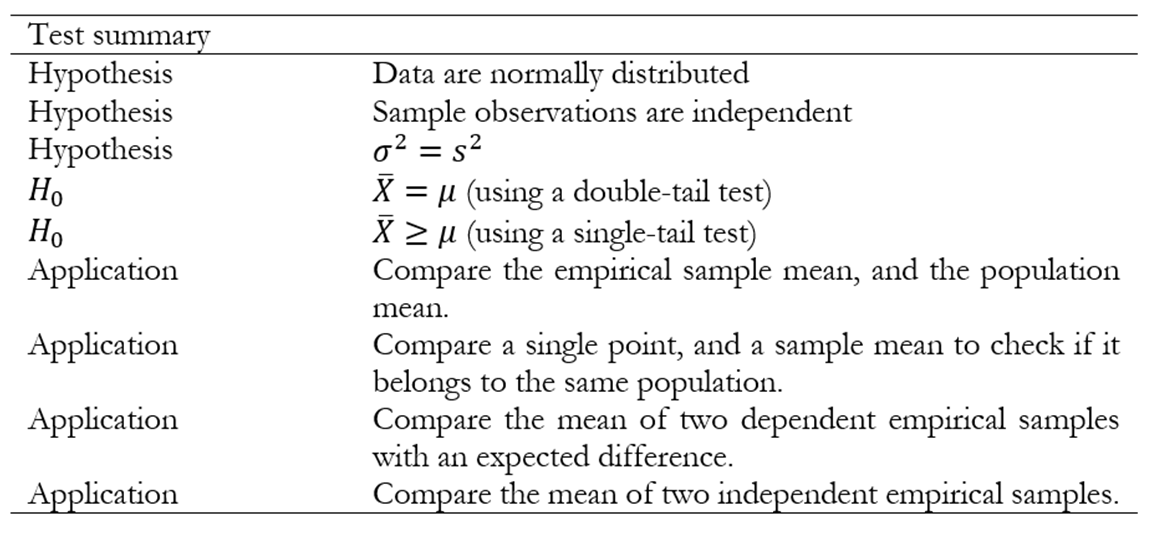
\includegraphics[width=0.7\textwidth]{SectionLetsMath/elemStat_figures/tab_tTest.png}
\captionsetup{type=table}
\caption{$t$-test summary.}
\label{tab_tTest}
\end{figure}

\subsection{$\chi^{2}$-test}
This test is used to check if a sample is distributed according to a given statistical distribution. The distribution of the test is a $\chi^2$ distribution defined as:

\begin{equation}
\chi_k^2=\sum_{i=1}^{k}{x_i^2=x_1^2+\ldots+x_k^2}
\label{eq_chi2Distribution}
\end{equation}

$x_1,\ldots x_k$ are random variables normally distributed and $k$ is the number of degrees of freedom. To check if a sample fits a statistical distribution (e.g., a normal distribution), the events are divided into $k$ subset each one having an observed frequency $o_k$ (sample) and an expected frequency $e_k$ (from the distribution). The definition of the $k$ classes is very important. The more the classes, the more one can check the fit with a statistical distribution. A good rule is that \% of the classes has at least 5 items and no class is empty. The statistic of the test is calculated as follows:

\begin{equation}
s=\sum_{i}^{k}\frac{\left|o_i-e_i\right|^2}{e_i}
\label{eq_chi2test}
\end{equation}

The value $s$ is, then, compared to the value of a random variable $\chi^2\ $ distributed with $n-1$ degrees of freedom. The greater the value of $s$, the greater the gap with the theoretical distribution. To quickly compare the obtained value of $s$, one defines a confidence interval $\alpha$, i.e. the maximum $p$-value accepted and the value of the degree of freedoms (i.e. the number of independent variables). The hypothesis is discarded, from the definition of the $p$-value, when ${s\geq\ \chi}_{dof}^2$. Note that the value $\alpha=0.1$ is the most restrictive test since it considers a smaller region of acceptance than the other (the non-acceptance region is 10\% of the whole data distribution). The hypothesis about the data and $H_0$ of the test are summarised in Table \ref{tab_Chi2}.


% INSERT tab_Chi2
\begin{figure}[hbt!]
\centering
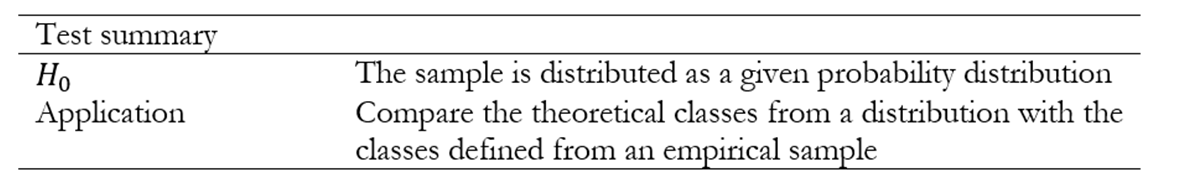
\includegraphics[width=0.9\textwidth]{SectionLetsMath/elemStat_figures/tab_Chi2.png}
\captionsetup{type=table}
\caption{$\chi^2$ test summary}
\label{tab_Chi2}
\end{figure}

\subsection{F-test}
This test aims at checking if two samples are normally distributed with the same variance. The statistics of this test is distributed as a Fisher-Snedecor distribution.
\begin{equation}
F=\frac{\frac{N_1}{m}}{\frac{N_2}{n}}
\label{eq_FisherDistribution}
\end{equation}

Where $N_1$ and $N_2$ are independent random variable $\chi^2$ distributed with $m$ and $n$ degrees of freedom. The test assumes $X$ and $Y$ are normally distributed. $X$ has $n$ samples and $Y$ has $m$ samples. The null hypothesis is $H_0=\sigma_X^2=\sigma_Y^2$. The statistic follows a Fisher distribution with $n-1$ and $m-1$ degrees of freedom:
\begin{equation}
F=\frac{S_X^2}{S_Y^2}
\label{eq_FisherTest1}
\end{equation}
The value of $F$ can be easily calculated having a dimensional space a number of $p$ parameters considering the sum of the squared residuals.
\begin{equation}
F=\frac{\left(\frac{SSR_X-SSR_Y}{p_X-p_Y}\right)}{\frac{SSR_Y}{n-p_Y}}
\label{eq_FisherTest2}
\end{equation}
The summary of the $F$-test is presented in Table \ref{tab_Ftest}.

% INSERT tab_Ftest
\begin{figure}[hbt!]
\centering
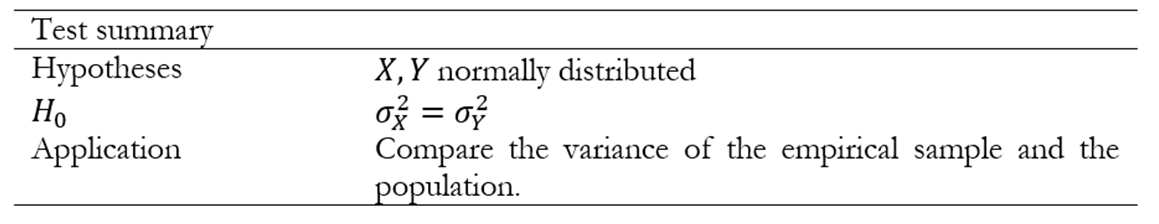
\includegraphics[width=0.9\textwidth]{SectionLetsMath/elemStat_figures/tab_Ftest.png}
\captionsetup{type=table}
\caption{F-test summary.}
\label{tab_Ftest}
\end{figure}

\section{Time series analysis} \label{secTimeSeries}


A time series (TS) is a series of the realisation of a random variable measured at constant time intervals. Time series can be used to forecast future values or to classify the realisations according to the properties of the TS (e.g., the seasonality). Even if both these applications sound intuitive, there is a lot of theory and math behind TSs. The entire theory of TS analysis is based on statistics.\par

The aim of TS analysis is the definition of a PDF describing the realisation of the events over time. Sometimes observations are some way linked to the others. This concept can be easily recognised thinking about the “continuity” of the nature around us (this is somehow related to the Principle of Least Action, already introduced in chapter \ref{sect_supplyChainPhysics}). Besides, it may exist a seasonality involving observations distant in the time (e.g. every summer is warmer than every winter). All these aspects drop the hypothesis of the independence of the observed variable that is commonly used in statistics to built simpler models. Under the independence hypothesis, it is possible to assume that the joint PDF of $X_1,\ldots,X_n$ random variables equals $f(x_1,\ldots,x_n)=\prod_{i=1}^{n}{f(x_i)}$. This is not true for TSs, and our work will get harder.\par

Since it is easy that each observation of a TS may depend on the previous: there is a sort of “influence” between them (in general, we can say that a TS has \textit{memory}). This is good news since it suggests that we could check historical values to make forecasts, that is one of our purposes.\par

TS are modelled as stochastic processes; for this reason, we introduce the notation indicating $X(\omega,t)$, where $X$ is the stochastic process. A TS behaves as a set of events $\omega$, one for each $t$ step, generated by $X(\omega,t)$. The random variable $X_t$ models the event at each time period $t$. Figure \ref{fig_stochProcess} shows the inputs and outputs of a stochastic process. We aim at describing the generating process $X(\omega,t)$ modelling the behaviour of the process to make forecasts.

% INSERT fig_stochProcess
\begin{figure}[hbt!]
\centering
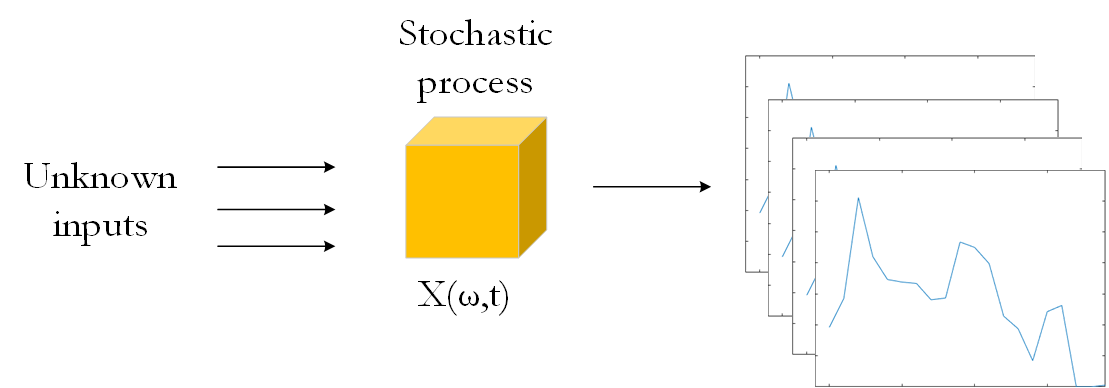
\includegraphics[width=0.9\textwidth]{SectionLetsMath/elemStat_figures/fig_stochProcess.png}
\captionsetup{type=figure}
\caption{Representation of a stochastic process.}
\label{fig_stochProcess}
\end{figure}


When modelling a TS as a stochastic process, there is a limit. A TS is composed of a single observation for each couple $(\omega,t)$. This is equal to have each event at a time $t$ represented by a single record (as having a single TS of the n represented in Figure \ref{fig_ACFPACF}). In practice, a single observation $X(t)$ is assumed to be representative of the entire event $\omega$ at time $t$. \footnote{The package logproj provides methods to deal with time series \href{https://github.com/aletuf93/logproj/blob/master/logproj/stat_time_series.py}{here}.
}

\subsection{Time series decomposition} \label{secTimeSeriesDecomposition}
TS decomposition is one of the approaches used to estimate the parameters of a stochastic process. The first assumption is made on how the stochastic process works. It is assumed it generates the TS based on three independent components.
\begin{itemize}
    \item A trend component $T(t)$;
    \item A seasonal component $S(t)$;
    \item A residual (random) component $R(t)$.
\end{itemize}

The literature proposes two models to mix these components. An additive (see equation \ref{eq_additiveTS}) and a multiplicative model (see equation \ref{eq_multiplicativeTS}). Figure \ref{fig_addMulTS} illustrates two realisations of an additive a multiplicative model.\footnote{The source code of Figure \ref{fig_addMulTS} is available \href{https://github.com/aletuf93/logproj/blob/master/examples/03.\%20Statistics.ipynb}{here}.}

\begin{equation}
X\left(t\right)=T\left(t\right)+S\left(t\right)+R(t)
\label{eq_additiveTS}
\end{equation}

\begin{equation}
X\left(t\right)=T\left(t\right)\times S\left(t\right)\times R(t)
\label{eq_multiplicativeTS}
\end{equation}

% INSERT fig_addMulTS
\begin{figure}[hbt!]
\centering
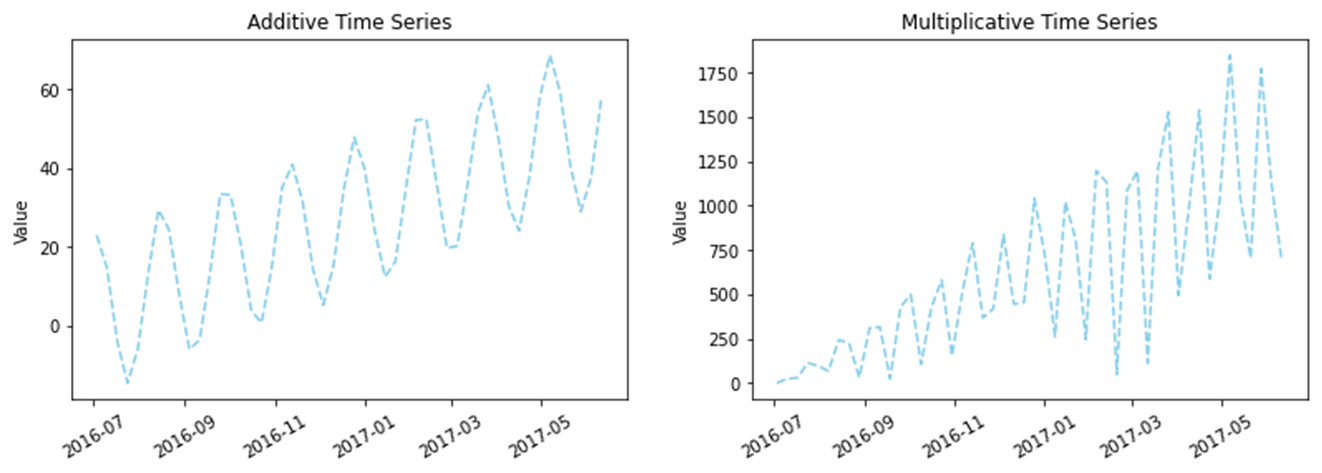
\includegraphics[width=0.9\textwidth]{SectionLetsMath/elemStat_figures/fig_addMulTS.png}
\captionsetup{type=figure}
\caption{Comparison between additive and multiplicative time series}
\label{fig_addMulTS}
\end{figure}

For the sake of brevity, the following paragraphs consider a TS modelled through additive model (see equation \ref{eq_additiveTS}) given that a multiplicative series can be transformed into an additive one using a logarithm transformation.

\begin{equation}
\begin{split}
    \log{\left(X\left(t\right)\right)} & =\log{\left(T\left(t\right)\times S\left(t\right)\times R\left(t\right)\right)}=\\
    & =\log{(T(t))+\log{(S(t))+\log{R(t))}}}\\
\end{split}
\label{eq_additiveMultiplicativeTransform}
\end{equation}

For this reason, all the techniques here presented are applicable to multiplicative models (see equation \ref{eq_multiplicativeTS}) too. In practice, one can fit both of them and measure their goodness of fit choosing the model which better describe the empirical measurements. 

An option to fit an additive model is to get the trend component of the series as a linear regression model fitted by ordinary least square (OLS\footnote{Section \ref{secLinearRegression} provides additional details of the OLS method.}). The result is a function $T\left(t\right)=mt+q$ where $m$ is the angular coefficient and $q$ is the intercept of the straight line best approximating the trend of $X(t)$. Alternatively, the trend can be estimated using a smoothing function, for example, using a Moving Average (MA) with a time window equal to the seasonality of $X(t)$\footnote{Sometimes, the seasonality of $X(t)$ is unknown. Section \ref{secFourier} shows how to detect the seasonality of a TS.}. Equation \ref{eq_trendTS} illustrates the formula of the MA; the time window is equal to $2h+1$ (e.g., $2h+1=7$ for a weekly seasonality of a time series having one sample per day).

\begin{equation}
T_t=\frac{1}{2h+1}\sum_{i=t-h}^{t+h}X_i
\label{eq_trendTS}
\end{equation}

Once the trend component T(t) has been extracted, the residual part (see Figure \ref{fig_extractedTrend})  of the TS equals\footnote{The source code of Figure \ref{fig_extractedTrend} is available \href{https://github.com/aletuf93/logproj/blob/master/examples/03.\%20Statistics.ipynb}{here}.}: 

\begin{equation}
S(t)+R(t)=X(t)-T(t)
\label{eq_extractedTrend}
\end{equation}

% INSERT fig_extractedTrend
\begin{figure}[hbt!]
\centering
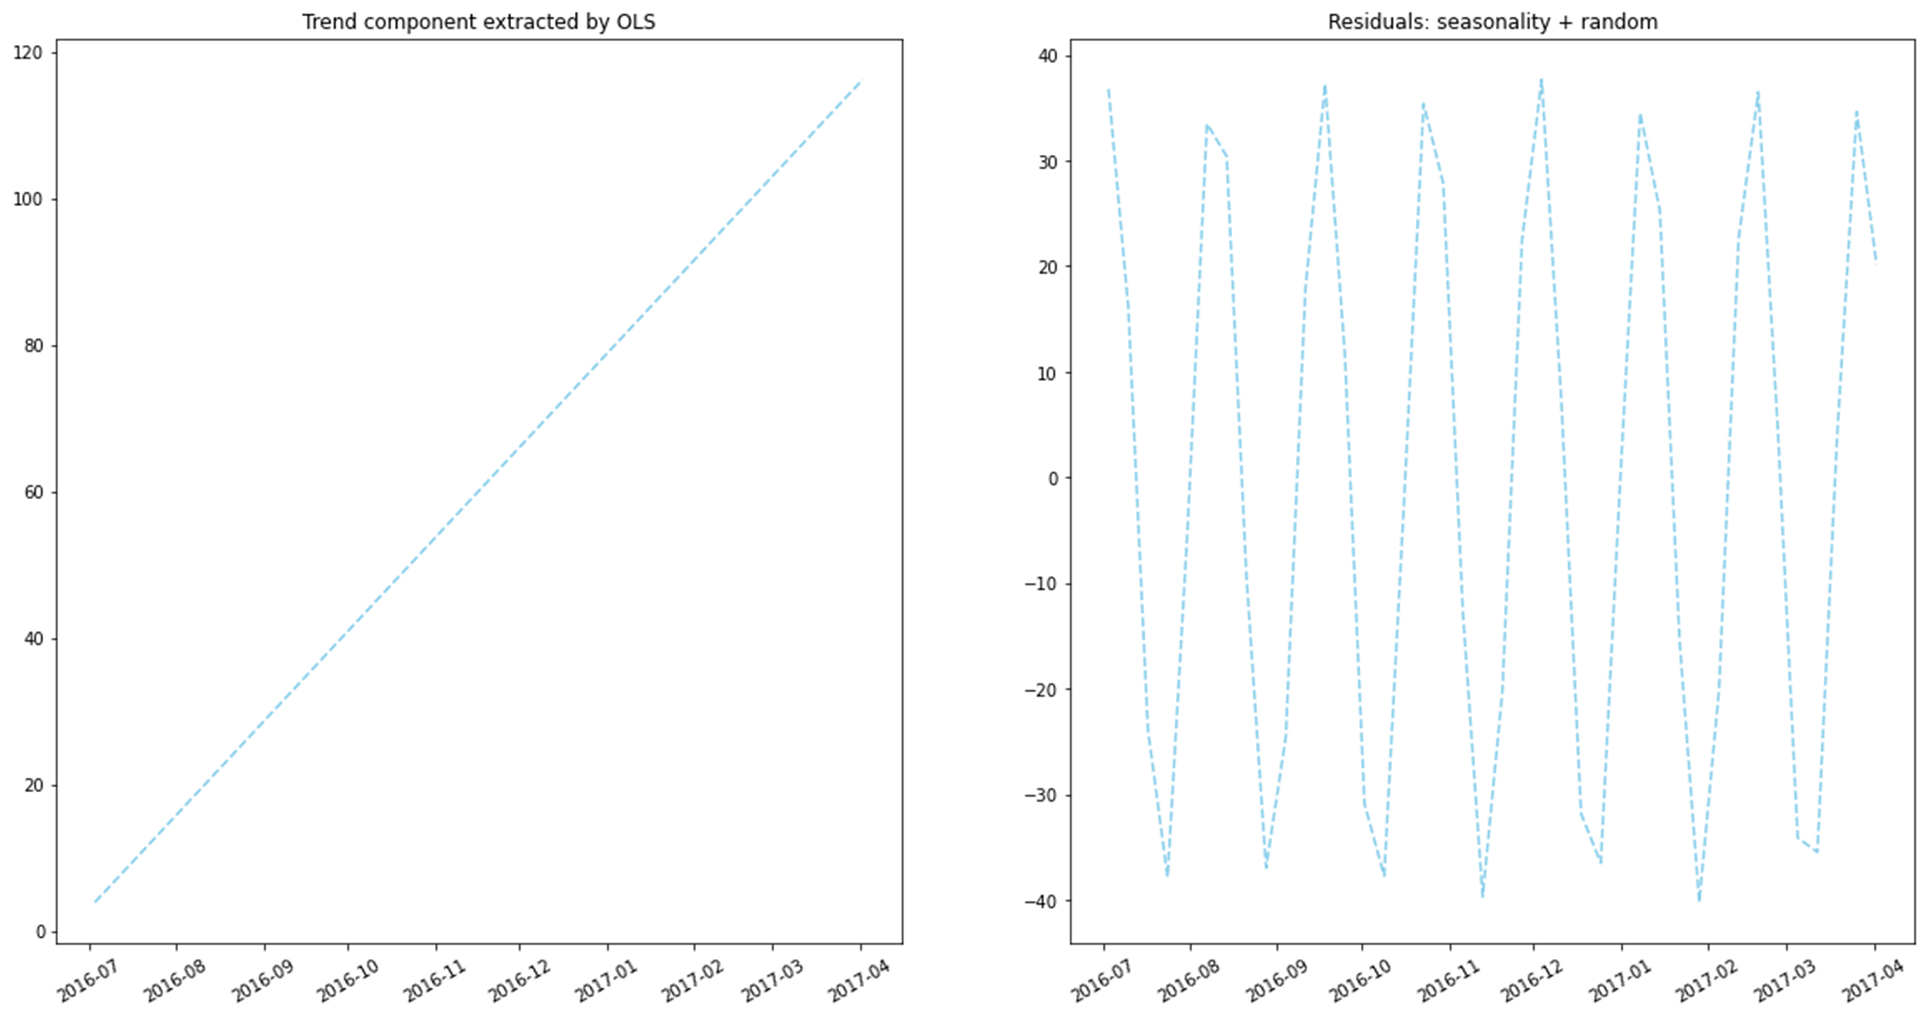
\includegraphics[width=0.9\textwidth]{SectionLetsMath/elemStat_figures/fig_extractedTrend.png}
\captionsetup{type=figure}
\caption{Extraction of the trend component from the TS.}
\label{fig_extractedTrend}
\end{figure}

To estimate the seasonal component $S(t)$ averaging is performed on the residual series $S\left(t\right)+R(t)$. Averaging works by grouping all the observation of the same seasonal period and applying average on it. The resulting value defines $S_t$. It is necessary to know the seasonality period to perform averaging (see Figure \ref{fig_averaging}). This can be done by the visualisation of the graphs or analytically using the Fourier transform analysing the frequency domain of the TS (see Section \ref{secFourier}).

% INSERT fig_averaging
\begin{figure}[hbt!]
\centering
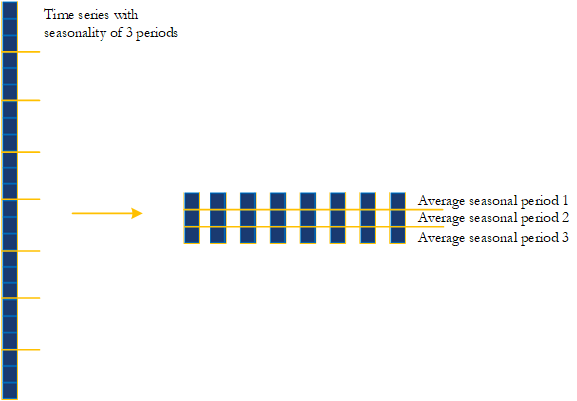
\includegraphics[width=0.9\textwidth]{SectionLetsMath/elemStat_figures/fig_averaging.png}
\captionsetup{type=figure}
\caption{Visualisation of the averaging method to estimate $S(t)$}
\label{fig_averaging}
\end{figure}

The residuals $R_t$ are obtained, again, by subtraction. If the residuals are randomly distributed, our model is interpreting the behaviour of the TS correctly. Otherwise, if the residuals show a pattern,  the estimation of $T(t)$ and $S(t)$ need more accuracy, or the choice of additive or multiplicative model is wrong. Figure \ref{fig_extractedSeasonality} shows the seasonal component and residuals. The residuals are randomly distributed, and it is possible to conclude that the decomposition process worked properly. Nevertheless, their magnitude is significant; collecting a higher number of samples would help in practice to reduce their magnitude and better detect the seasonality\footnote{The source code of Figure \ref{fig_extractedSeasonality} is available \href{https://github.com/aletuf93/logproj/blob/master/examples/03.\%20Statistics.ipynb}{here}.}.

% INSERT fig_extractedSeasonality
\begin{figure}[hbt!]
\centering
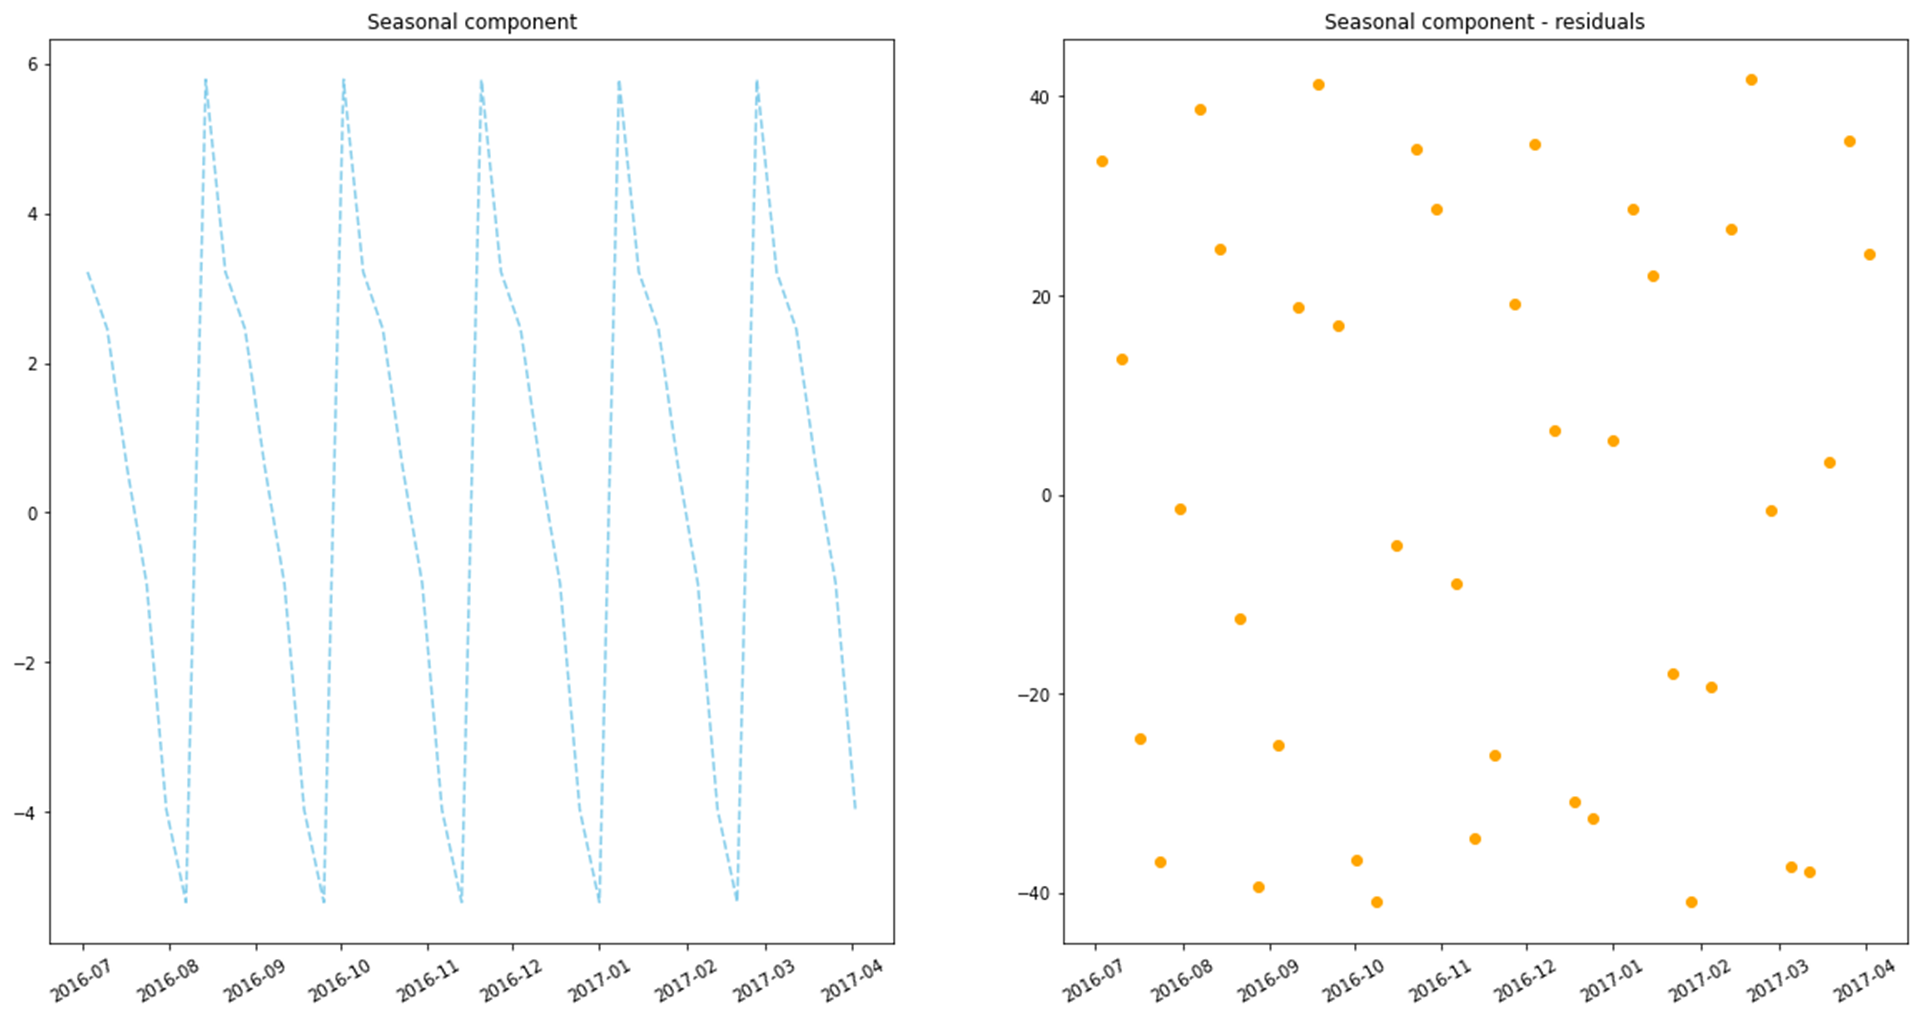
\includegraphics[width=0.9\textwidth]{SectionLetsMath/elemStat_figures/fig_extractedSeasonality.png}
\captionsetup{type=figure}
\caption{Extraction of the seasonal component from the TS.}
\label{fig_extractedSeasonality}
\end{figure}

\subsection{ARIMA models} \label{secARIMA}

A more complex way to model TSs comes from the autoregressive and moving average (ARIMA) models. These models are based on the Wold’s decomposition theorem stating that “Every covariance-stationary time series $X(t)$ can be written as the sum of two time series, one deterministic and one stochastic. In other words, given a stationary stochastic process $X_t$ with mean value $\mu$ it is always possible to decompose the process into $X_t=Z_t+V_t$ such that $cov\left(Z_t,X_t\right)=0$. In particular:

\begin{equation}
V_t=\mu+\sum_{j=1}^{+\infty}\left[\alpha_j\sin{\left(\omega_jt\right)}+\beta_j\left(\omega_jt\right)\right],0\le\omega_j\le\pi
\label{eq_ARIMAautoregressive}
\end{equation}

\begin{equation}
Z_t=\sum_{j=0}^{+\infty}{\psi_ja_{t-j}}
\label{eq_ARIMAmovingaverage}
\end{equation}

Equation \ref{eq_ARIMAautoregressive} models the autoregressive component where $V_t$ is the deterministic part of the model; $\omega_j$ is a fixed frequency and $\alpha_j$ and $\beta_j$ are uncorrelated white noise \footnote{A white noise process $a_t \sim WN\left(0,\sigma_a\right)$ is such that: $E\left(a_t\right)=0$; $Var\left(a_t\right)=\sigma_a^2$; $cov\left(a_t,a_{t-k}\right)=0 \forall t\in T,\ k\neq0$.} processes. $Z_t$ (see equation \ref{eq_ARIMAmovingaverage}) is the stochastic process and it is a moving average of infinity order where $a_t$ is the prediction error. In practice, a consequence of the Wold’s theorem is that once a TS has been transformed into a stationary TS it can be modelled as a linear function of a white noise process.A stochastic process is stationary when it has constant mean and variance and its autocovariance only depends on the time lag k (not by the time t). Using equations:

\begin{equation}
\begin{split}
    E\left(X_t\right)=\mu<\infty,\ & \forall t\in T\\
    Var\left(X_t\right)=\sigma_X^2<\infty,\ & \forall t\in T\\
    Cov\left(X_t,X_{t-k}\right)=\gamma_k<\infty,& \forall k\in T\\
\end{split}
\label{eq_stationarity}
\end{equation}

If these conditions are met, it is possible to apply an ARIMA model to a TS to model it as a sum of an autoregressive process (AR) (derived from $V_t$) and a moving average process (MA) (derived from $Z_t$). In general, a TS is not stationary, and it is not possible to directly apply ARIMA models. A trend in the series, for example, violates equations \ref{eq_stationarity}. For this reason, detrending is almost always necessary to get a series meeting the stationarity condition. Box and Jenkins \cite{Box1970} introduced some transformation to deal with non-stationary TS (see Table \ref{tab_transformation}).


% INSERT tab_transformation
\begin{figure}[hbt!]
\centering
\includegraphics[width=0.9\textwidth]{SectionLetsMath/elemStat_figures/tab_transformation.png}
\captionsetup{type=table}
\caption{Transformations to obtain a stationary TS}
\label{tab_transformation}
\end{figure}


Once the TS has been transformed into a stationary one, it is possible to fit an ARIMA model choosing adequate parameters $p$ and $q$, indicating the autoregressive (AR) order and the moving average (MA) order. At this purpose, the autocorrelation functions PACF, and ACF are studied. The echo phenomenon exemplifies the effect of the autocorrelation. After a certain amount of time units (i.e. time lags), the echo overlaps original message altering the sound waveform. The echo of the signal of a TS is the seasonality (i.e. certain weeks or months of the year where the TS is amplified). To detect this phenomenon, we use ACF and PACF as defined in Section \ref{secCovarianceCorrelation}. Figure \ref{fig_nonStationaryTS} illustrates a TS with its ACF and PACF, while Figure \ref{fig_StationaryTS} illustrates the same series with ACF and PACF after detrend using OLS.\footnote{The source code of Figure \ref{fig_nonStationaryTS}, and Figure \ref{fig_StationaryTS} is available \href{https://github.com/aletuf93/logproj/blob/master/examples/03.\%20Statistics.ipynb}{here}.}.


% INSERT fig_nonStationaryTS
\begin{figure}[hbt!]
\centering
\includegraphics[width=0.9\textwidth]{SectionLetsMath/elemStat_figures/fig_nonStationaryTS.png}
\captionsetup{type=figure}
\caption{ACF and PACF of the original TS.}
\label{fig_nonStationaryTS}
\end{figure}

% INSERT fig_StationaryTS
\begin{figure}[hbt!]
\centering
\includegraphics[width=0.9\textwidth]{SectionLetsMath/elemStat_figures/fig_StationaryTS.png}
\captionsetup{type=figure}
\caption{ACF and PACF of the detrended TS.}
\label{fig_StationaryTS}
\end{figure}

Stationarity can be tested using the Dickey-Fuller test for stationarity. Alternatively, a series is stationary if its ACF and PACF decrease, i.e. the ACF, and PACF correlograms tends to zero asymptotically. The last significant value of the PACF is used for the parameter $p$ (the order of the AR model) while the last significant lag value of the ACF is used for the parameter $q$ (the order of the MA model). In this case, we would try to fit a model ARIMA(1,1). Note that if the PACF goes to zero immediately, the most important value is '1' (since a TS is always autocorrelated with itself at the same time lag). In this case, $T_t$ is constant and no waveform (i.e. seasonality) exists. When the ACF suggests no values, instead, '0' should be the order used for $q$.

\subsection{Fourier transform} \label{secFourier}

All the models introduced in the previous paragraphs assume that a seasonality exists and its lag is defined (or can be defined analysing the graph of the time series). Nevertheless, in some cases, it may be necessary to have analytical methods to study the seasonality of a series. For this reason, we introduce the spectrum analysis and the Fourier transform. Spectrum analysis is a methodology widely used in telecommunication for the analysis of signals. Signals (analogue or digital) are usually periodic and characterised by a period $\tau$, due to their sinusoidal behaviour. A periodic (i.e. sinusoidal) signal (see Figure \ref{fig_signal}) can be modelled as\footnote{The source code of Figure \ref{fig_signal} is available \href{https://github.com/aletuf93/logproj/blob/master/examples/03.\%20Statistics.ipynb}{here}.}.:

\begin{equation}
y=S(t)=Asin(\omega t+\phi)
\label{eq_signal}
\end{equation}


% INSERT fig_signal
\begin{figure}[hbt!]
\centering
\includegraphics[width=0.9\textwidth]{SectionLetsMath/elemStat_figures/fig_signal.png}
\captionsetup{type=figure}
\caption{Model of a periodic signal.}
\label{fig_signal}
\end{figure}

Where $A$ is the amplitude of the signal, $\phi$ is the phase (translation on the time axis). $\omega$ is the angular velocity, i.e. the number of periods within a time interval of $2\pi$. The frequency $f$ is linked to the period $\tau$ and to the angular velocity $\omega$ by the following.

\begin{equation}
f=\frac{1}{\tau}=\frac{\omega}{2\pi}
\label{eq_frequency}
\end{equation}

Given the equation \ref{eq_frequency}, the $S\left(t\right)$ can be expressed in terms of the frequency $f$.

\begin{equation}
y=Asin(f2\pi t+\phi)
\label{eq_frequency2}
\end{equation}

Telecommunication uses different strategies to transmit signals avoiding losses during the transmission. It often happens to transmit signals digitally. When the source is analogue (i.e. continuous bu nature) the signal has to be sampled. Sampling means removing part of the signal, but if it is performed correctly, it does not remove any information. Sampling is performed at a fixed frequency $f_s$ i.e., each sample has a distance in time from the previous one equal to $T$. To properly maintain the level of information of a signal, $f_s$ must be chosen adequately. The Nyquist-Shannon sampling theorem demonstrates that given a periodic signal $g\left(t\right)$ with maximum frequency $f_M$ (i.e. a bandwidth $[0,f_M]$), can be completely defined (i.e. without loss of information) using a sampling frequency $f_s\geq2f_M$ i.e. a sampling step $t_s\le\frac{1}{2f_M}$. Figure \ref{fig_signalsampling} shows the samples of a signal generated by a continuous source.\footnote{The source code of Figure \ref{fig_signalsampling} is available \href{https://github.com/aletuf93/logproj/blob/master/examples/03.\%20Statistics.ipynb}{here}.}


% INSERT fig_signalsampling
\begin{figure}[hbt!]
\centering
\includegraphics[width=0.9\textwidth]{SectionLetsMath/elemStat_figures/fig_signalsampling.png}
\captionsetup{type=figure}
\caption{signal with $N=600$ and $f_s\ =800\ $ Hz.}
\label{fig_signalsampling}
\end{figure}

The original signal can be recreated using the Fourier transform on the sampled signal investigating its behaviour in the frequency domain. The signal is expected to have a maximum original frequency of 400\ Hz (i.e. it has been sampled correctly, accordingly with the Nyquist-Shannon theorem).\par

The Fourier theorem states that any periodic function $x(t)$ may be expressed as a sum of infinite terms of sine and cosine terms (called Fourier series), each of them with a specific amplitude and phase complex coefficient $c_n$ called the Fourier coefficient. 

\begin{equation}
c_n=\frac{1}{T_0}\int_{T_0}{x\left(t\right)e^{-2\pi n f_0t\ }dt}
\label{eq_FourierCoefficients}
\end{equation}

Fourier transform is used to calculate the values of $c_{n\ }$.

\begin{equation}
X\left(f\right)=F\left\{x\left(t\right)\right\}=\int_{-\infty}^{+\infty}{x\left(t\right)e^{-j2\pi ft}}dt
\label{eq_Fouriertransform}
\end{equation}

The representation of these frequencies is obtained through amplitude and phase spectra which represents the absolute value and the argument of the complex coefficients $c_n$. The amplitude spectrum of the sampled signal is shown in Figure \ref{fig_Fourier}.\footnote{The source code of Figure \ref{fig_Fourier} is available \href{https://github.com/aletuf93/logproj/blob/master/examples/03.\%20Statistics.ipynb}{here}.}

% INSERT fig_Fourier
\begin{figure}[hbt!]
\centering
\includegraphics[width=0.9\textwidth]{SectionLetsMath/elemStat_figures/fig_Fourier.png}
\captionsetup{type=figure}
\caption{Amplitude spectrum of the signal.}
\label{fig_Fourier}
\end{figure}

The amplitude spectrum shows that two sinusoids with frequency 50 and 80 Hz generate the original signal; the harmonics are showed on the chart. Looking at the source code, the generating function of the samples was $y=\sin{\left(50 \times 2\pi x\right)}+0.5\sin(80\times2\pi x)$ which confirms the results of the transform.\par

Dealing with time series, we can use the Fourier transform to investigate if a periodical signal can be used to model the seasonal component of the series. In particular, we are looking for $f$ of the model in equation \ref{eq_frequency}. Where $f$ can be reasonably be expressed in $week^{-1}$, i.e. $f^{-1}$ defines the length of a period, i.e. the length of the seasonality.\par

Time series are usually extracted from a database which is digitalised and already sampled (e.g. daily/monthly/yearly) so it is difficult to define a priori the number of samples. This can be defined by different grouping strategy (e.g., daily/weekly). It is, anyway, essential to verify if the number of samples allows for resilient inference on the seasonality.\par

To perform Fourier analysis on a time series, it is necessary to detrend it first, as shown in \ref{secTimeSeriesDecomposition}. At this stage, the time series fluctuates around its mean with an unknown frequency and can be modelled as a periodic signal using the Fourier transform. 

\section{Bayesian Statistics} \label{secBayesTheorem}
The statistics illustrated so far is entirely based on the observation of physical phenomena. The events are observed, measured, and the outcomes of these experiments are analysed in a \textit{frequency} fancy. The values occurring the most are the most probable. This statistics is based on the frequentist approach. Sometimes we do not have the possibility of measure the variable of our interest; nevertheless, we have \textit{beliefs} on the behaviour of this variable, and we may be interested in expressing these believes in terms of probability. \par

For example, when measuring partial data of a total quantity, we have the belief that the total quantity is higher than the measured one. We can measure a variable using two different measurement systems, having the belief that one outperforms the other under certain circumstances. We may start an experiment having prior beliefs on the expected outcome. Bayesian statistics helps in all these situations. The main theorem of Bayesian statistic is the Bayes’ theorem:

\begin{equation}
P\left(A\middle| B\right)=\frac{P(A\cap B)}{P(B)}=\frac{P(B|A)}{P(B)}
\label{eq_bayesTheorem}
\end{equation}

This theorem is also known as the theorem of conditional probability. While frequentist statistics assume $A$, and $B$ being events; the Bayesian approach defines $A$ as the prior, and $B$ the posterior. The prior $A$ defines the belief we have before an experiment starts, i.e. before starting collecting measurement. The information of the measurements is, then, contained in the posterior $B$. Bayesian statistics aims at matching the prior and the posterior by assuming that the prior $A$ is true. In practice, we have observations, we expect they behave as $A$ describes, but we observe a behaviour $B$, and we need to correct it. Bayesian statistics is the perfect tool to match prior models with posterior empirical observations to predict their behaviour. Bayesian tools work similarly to machine learning models since all machine learning models aim at the definition of a joint probability distribution between a prior and a posterior. For this reason, these methods are presented in \ref{secBayesianMethods}.



\section*{Further reading}
Supplementary reading materials can be found in \cite{Sauter2002}, \cite{Ruppert2015}, \cite{Brandt2014}, \cite{Heibergerer2015}.

%\clearpage
\bibliographystyle{ieeetr}
\bibliography{SectionLetsMath/elemStat_ref}



\chapter{Dimensionality reduction}{}

%citazione introduttiva
\epigraph{\textit{We need data, but maybe not all of them.}}{}

Databases, Internet of Things, big data provide tons of data per second. There is an obvious obstacle in processing all of them since a large computational power and a lot of storage memory are needed. Besides, a portion of this data does not provide useful information since it may have a fixed value or an extremely high correlation with the other data. We introduce dimensionality reduction strategies to smooth the process of data processing and to get information fastly and efficiently. These strategies aim at getting the highest level of information possible using the lowest amount of input data.\par

Let assume that data from our sources is organised in a dataset $X_{N\times P}$ having $N$ observation (rows) and $P$ features (columns). Each observation describes the realisation of a phenomenon characterised by the $P$ features. Dimensionality reduction aims at explaining the information of each row in $X$ using only K features, with $K<P$. To meet this goal, features can be:

\begin{itemize}
    \item extracted (i.e. the $P$ features are transformed to explain the majority of the information in $X$);
    \item selected (i.e. a subset $K$ of $P$ explains the majority of the information in $X$). 
\end{itemize}

The following paragraphs explore techniques belonging to these two methodologies.\footnote{The package logproj provides methods to deal with time series \href{https://github.com/aletuf93/logproj/blob/master/logproj/ml_dimensionalityReduction.py}{here}.} 

\section{Feature extraction}
The most common feature extraction strategy is the principal component analysis (PCA); this section introduces it using the singular value decomposition (SVD) to decompose a dataset $X$. SVD and PCA can be used when a learning table is composed of many columns (e.g. with image recognition or dummy columns from an initial dataset containing categorical variables converted into binary features). SVD and PCA use eigenvalues and eigenvector to transform the features space reducing overfitting. Eigenvectors are defined as vectors whose direction does not change when a linear transformation is applied to them. Eigenvalues are the scalar used to transform the eigenvectors. Given a matrix $A$, we can write:

\begin{equation}
Ax-\lambda x=0
\label{eq_eigenvaluesEigenvectors}
\end{equation}
Where x is the eigenvector of A and $\lambda$ are the eigenvalues of A.

\subsection{Singular Value Decomposition (SVD)} \label{secSVD}
In general, any matrix $X_{N,P}$ can be decomposed into a product of a mixing matrix $U_{N,K}$ and a dictionary matrix $V_{P,K}$ such that:
\begin{equation}
X=UV^T
\label{eq_SVD1}
\end{equation}

A row $x_i\in X$ is a linear combination (according to an entry $u_i\in U$) of the linearly independent elements $v_i\in V$. Singular value decomposition (SVD) is a matrix factorisation technique which decomposes a matrix $X$ into:

\begin{equation}
X_{N,P}=U_{N,K}D_{K,K}V_{P,K}^T
\label{eq_SVD2}
\end{equation}

Table \ref{tab_svd} shows the information content of the three matrices produced by the SVD.

% INSERT tab_svd
\begin{figure}[hbt!]
\centering
\includegraphics[width=0.9\textwidth]{SectionLetsMath/dimensionalityReduction_figures/tab_svd.png}
\captionsetup{type=table}
\caption{elements of the SVD.}
\label{tab_svd}
\end{figure}

\subsection{Principal Component Analysis (PCA)} \label{secPCA}
PCA aims at reducing  $X_{N,P}$ to $C_{N,K}$  with $K<P$ where $K$ is the number of orthogonal vectors used to explain the variability of $X$. The PCA projects the elements of $X$ in the $K$ directions defined by $V_K$ such that the variance of the $N$ observation is maximised along this direction. In practice, PCA projects the reference system of the $P$ variables onto a new Kdimensional coordinate system $V$. All the entries $x_i$ of the matrix $X_{\left(N,P\right)}$ are converted into the new reference system at $x_{i\left(1,P\right)}^Tv_{\left(P,1\right)}\ $ . PCA defines:

\begin{equation}
v_{\left(P,1\right)}=\arg\max_{v:\left|\left|v\right|\right|=1}{{\frac{1}{N}\sum_{i}\left(x_i^Tv\right)^2}}
\label{eq_PCA}
\end{equation}

It is necessary to remember that, before applying PCA:
\begin{enumerate}
    \item Data has to be centred; i.e. $X=X-{\bar{x}}^T$, since the equation \ref{eq_PCA} maximises the variance of the sample data.
    \item Data has to be standardised;  i.e. having the same variance of all the variables $P$. Otherwise, variables with higher (absolute) variances will overcome the others.
\end{enumerate}

In addition to these, the maximisation objective is constrained to $\left|\left|v\right|\right|=1$ for two reasons:

\begin{enumerate}
    \item We are only interested in the direction of the projection, not in its magnitude;
    \item Without this constraint, the maximisation objective would be unbounded.
\end{enumerate}

Let, now, express the maximisation function at:
\begin{equation}
\arg\max_{v:\left|\left|v\right|\right|=1}{{\frac{1}{N}v^TX^TXv}}
\label{eq_PCA1}
\end{equation}

Please note that the covariance matrix $S_{xx}$ equals $\frac{1}{N}X^TX$, then:

\begin{equation}
\arg\max_{v:\left|\left|v\right|\right|=1}{{v^TS_{xx}v}}
\label{eq_PCA2}
\end{equation}

By using Lagrangian multipliers $\lambda$, it is possible to express the maximisation function at:

\begin{equation}
\max{v^TS_{xx}v-\lambda(v^Tv-1)}
\label{eq_PCA3}
\end{equation}

It is then, possible proceed to calculate the stationary points, i.e. where the derivative of the function (regards to $v$) is equal to zero.

\begin{equation}
\frac{d}{dv}\left\{v^TS_{xx}v-\lambda\left(v^Tv-1\right)\right\}=v^TS_{xx}-\lambda v=0
\label{eq_PCA4}
\end{equation}

\begin{equation}
S_{xx}v=\lambda v
\label{eq_PCA5}
\end{equation}

We conclude that:
\begin{itemize}
    \item $v$ is the eigenvector of $S_{xx}$;
    \item $\lambda$ is the eigenvalue of $S_{xx}$.
\end{itemize}

It is, then, possible to conclude that the variance is maximised when $v$ is an eigenvector of $S_{xx}$ (i.e. the covariance matrix) corresponding to the largest eigenvalue $\lambda$. In practice, the PCA is performed using the sample covariance matrix $S_{xx}=\frac{1}{N-1}X^TX$ and the SDV of $X^TX$.

\begin{equation}
X^TX=\left(UDV\right)^T\left(UDV^T\right)=VD^TU^TUDV^T
\label{eq_PCA6}
\end{equation}
Since $U$ is orthogonal, $U^TU=I$, then:

\begin{equation}
X^TX=VD^TDV^T
\label{eq_PCA7}
\end{equation}

Since $D$ is a square matrix, $D^TD=D^2$, then:
\begin{equation}
\begin{split}
    X^TX=VD^2V^T \\
    V^TX^TXV=D^2 \\
    {\frac{1}{N-1}V}^TX^TXV={\frac{1}{N-1}D}^2 \\
    V^TS_{xx}V={\frac{1}{N-1}D}^2 \\
\end{split}
\label{eq_PCA8}
\end{equation}

Then:
\begin{itemize}
    \item The eigenvectors of $S_{xx}$ are the right-singular vectors $V$;
    \item The eigenvalues $\lambda_k$ (which are the variance of the components) are equal to $\frac{1}{N-1}d_k$, where $d_k$ are the squared singular values.
\end{itemize}

In conclusion, the PCA performs the SVD on the data covariance matrix $S_{xx}$, and it produces three outputs:
\begin{enumerate}
    \item The principal component directions, i.e. the right singular vectors $V_{K,P}$ of an SVD which are the eigenvectors of $X^TX$.
    \item The principal components, i.e. a matrix $C_{N,K}$, obtained projecting $X_{N,P}$ onto the principal components directions $V_{K,P}$ the left singular vectors $U_{N,K}$:
        \begin{equation}
        C_{N,K}=X_{N,P}V_{P,K}=UDV_{N,P}^TV_{P,K}=UD_{N,K}^T
        \label{eq_PCA9}
        \end{equation}
    Accordingly, $U$ (the left-singular value matrix) is the matrix of $u_j$ with the projections of the row vectors of $X$ in the new reference system (direction $v_j$) scaled by $d_j$. In practice, the PCA produces $k$ principal components $(k=1,\ldots,K)$ which are a linear combination of the original variables:
        \begin{equation}
        c_k=x_1u_1+\ x_2u_2+\ldots+x_Pu_P
        \label{eq_PCA10}
        \end{equation}
    \item The variance of each component, given by the eigenvalues $\lambda_k=1,\ldots,K$. This is obtained from the singular values in $D_{K,K}$.
        \begin{equation}
        var\left(c_k\right)=\frac{1}{N-1}d_k^2
        \label{eq_PCA11}
        \end{equation}
\end{enumerate}
	
	
The theory does not explain how to choose the number of PCs. This information can be obtained by building a curve showing the information content of each principal component. Figure \ref{fig_PCAinformation} presents this curve based on the data of the sample \textit{wine dataset}. The curve illustrates the percentage of the variance of the dataset $X$ given a certain number of components $K$. In this case, the dataset $X$ count 13 features, but the first six components are enough to explain 80\% of the variance of $X$.\footnote{The source code of Figure \ref{fig_PCAinformation} is available \href{https://github.com/aletuf93/logproj/blob/master/examples/05.\%20Dimensionality\%20Reduction.ipynb}{here}.
}	

% INSERT fig_PCAinformation
\begin{figure}[hbt!]
\centering
\includegraphics[width=0.8\textwidth]{SectionLetsMath/dimensionalityReduction_figures/fig_PCAinformation.png}
\captionsetup{type=table}
\caption{Cumulative curve of the information content of the principal components.}
\label{fig_PCAinformation}
\end{figure}

\subsection{Multi-dimensional scaling} \label{secMultiDimensionalScaling}
In some cases, we do not have a matrix $X_{N,P}$ with observations and features but a distance matrix $D_{N,N}$ expressing a pairwise distance between each observation, for a given feature. In this case, it is recommendable to turn he $D$ matrix into a $P$ one, but this involves the approximation of the distance values into a $K$-dimensional space.\par

Multidimensional scaling aims at this goal, considering a $D_{N,N}$ and finding a low-dimensional projection of the data such that a stress function is minimised.

\begin{equation}
    \min stress\left(X\right)=\ {\sum_{i\neq j}\left(d_{ij}-\left|\left|x_i-x_j\right|\right|\right)}^2
    \label{eq_MDS}
\end{equation}

\subsection{t-SNE}

t-SNE is a common technique when the number of features $P$ is high. This technique tries to separate the variables rather than combining their effect (as in PCA); also, it provides effective visualisation in low dimensional space (e.g., $K=2$).\par

t-SNE algorithm proceeds step by step, determining the similarity between each observation of the dataset $X$ according to the values of its features $P$. The similarity is measured as the distance between each observation and a Gaussian curve which is, then normalised to 1. Once all similarity values are calculated, a similarity matrix $D$ is defined.\par

All the observation are randomly scattered on the $K$-dimensional space, and their distance is measured as the distance between the observation and a $t$-distribution populating the matrix $D_t$. At this stage, points are re-organised in the $K$-dimensional space one by one to make $D_t$ similar to $D$ defining compact clusters.

\section{Feature selection}
Feature selection strategies implement heuristics to define a subset of the P features to train learning algorithms. The following paragraphs illustrate these strategies.

\subsection{Selection by correlation}
The correlations between the features of the input dataset $X$ are values to check carefully before training a learning algorithm. If two features are highly correlated, it may be necessary to exclude one of them since the other already describes the variability of the dataset. The correlation matrix is used for this purpose to identify the correlation coefficients of all the possible couples of variables. Figure \ref{fig_corrMatrix} shows an example of a correlation matrix from the wine dataset using different colour gradients to highlight positive and negative correlations.\footnote{The source code of Figure \ref{fig_corrMatrix} is available \href{https://github.com/aletuf93/logproj/blob/master/examples/05.\%20Dimensionality\%20Reduction.ipynb}{here}.}

% INSERT fig_corrMatrix
\begin{figure}[hbt!]
\centering
\includegraphics[width=0.8\textwidth]{SectionLetsMath/dimensionalityReduction_figures/fig_corrMatrix.png}
\captionsetup{type=table}
\caption{Correlation matrix of the wine dataset.}
\label{fig_corrMatrix}
\end{figure}

Another strategy based on the correlation consists of training an algorithm only with a subset of variables having a minimum value of correlation with the target variable. Figure \ref{fig_selectCorr} shows the correlation behaviour of the features of the \textit{wine dataset} with the target variable. The plot shows the number of features (y-axis) having a minimum correlation value (x-axis) with the target variable. One may decide to set a threshold of minimum correlation to work with a subset o variable resulting significantly correlated to the target variable (e.g. at least 30\% of correlation).\footnote{The source code of Figure \ref{fig_selectCorr} is available \href{https://github.com/aletuf93/logproj/blob/master/examples/05.\%20Dimensionality\%20Reduction.ipynb}{here}.}

% INSERT fig_selectCorr
\begin{figure}[hbt!]
\centering
\includegraphics[width=0.8\textwidth]{SectionLetsMath/dimensionalityReduction_figures/fig_selectCorr.png}
\captionsetup{type=table}
\caption{Number of features with a minimum correlation threshold with the target variable (wine dataset).}
\label{fig_selectCorr}
\end{figure}

\subsection{Selection by variance}
Another strategy is to select a subset of variables whose variance is above a certain level. The idea is the following: if a feature has a low variance, it does not add too much information to the dataset. All the features with variance equal to zero should be removed since they do not add any information to the dataset. Figure \ref{fig_selectVariance} illustrates the variance of the features of the \textit{wine dataset}. The majority of the features has a variance lower than 60\%.\footnote{The source code of Figure \ref{fig_selectVariance} is available \href{https://github.com/aletuf93/logproj/blob/master/examples/05.\%20Dimensionality\%20Reduction.ipynb}{here}.}

% INSERT fig_selectVariance
\begin{figure}[hbt!]
\centering
\includegraphics[width=0.8\textwidth]{SectionLetsMath/dimensionalityReduction_figures/fig_selectVariance.png}
\captionsetup{type=table}
\caption{Number of features above a minimum variance threshold (wine dataset).}
\label{fig_selectVariance}
\end{figure}

\subsection{Selection by Lasso coefficients}
Lasso regression (further details in Section \ref{secLassoRegression}) is a prediction model that extends the linear regression which embeds a feature selection strategy. It automatically identifies a coefficient for each feature, shrinking the feature according to its relative importance. The coefficients of a Lasso regression can be used to select only the important features. Figure \ref{fig_LassoPath} shows the graph with the feature coefficients of the \textit{wine dataset} (on the y-axis) depending on the tuning hyperparameter $\alpha$ of the Lasso on the x-axis and the value of the coefficients.\footnote{The source code of Figure \ref{fig_LassoPath} is available \href{https://github.com/aletuf93/logproj/blob/master/examples/05.\%20Dimensionality\%20Reduction.ipynb}{here}.} 

% INSERT fig_LassoPath
\begin{figure}[hbt!]
\centering
\includegraphics[width=0.8\textwidth]{SectionLetsMath/dimensionalityReduction_figures/fig_LassoPath.png}
\captionsetup{type=table}
\caption{Lasso shrinkage coefficients graph depending on the value of the hyperparameter $\alpha$ (wine dataset).}
\label{fig_LassoPath}
\end{figure}

The graph shows that many coefficients are kept to zero up to some values of $\alpha$. Features can be selected using Lasso identifying a minimum threshold on the value of the coefficients, pinpointing relative importance of the underlying attributes. Figure \ref{fig_selectLasso} illustrated the number of features selected from the \textit{wine dataset} by using different thresholds on the value of the coefficients.\footnote{The source code of Figure \ref{fig_selectLasso} is available \href{https://github.com/aletuf93/logproj/blob/master/examples/05.\%20Dimensionality\%20Reduction.ipynb}{here}.} 


% INSERT fig_selectLasso
\begin{figure}[hbt!]
\centering
\includegraphics[width=0.8\textwidth]{SectionLetsMath/dimensionalityReduction_figures/fig_selectLasso.png}
\captionsetup{type=table}
\caption{Number of features above a minimum lasso coefficient threshold (wine dataset).}
\label{fig_selectLasso}
\end{figure}

\subsection{Selection by using a decision tree}
A decision tree trains a predicting model branching on the value of a variable defining a tree structure (further details in Section \ref{secDecisionTrees}). The most important features can be selected, evaluating which of them appears the most as a branching variable. Identifying a minimum threshold on the number of times a feature appears as a branching variable works as a feature selection strategy.

\subsection{Forward Stepwise selection}

Forward stepwise selection uses the principles of the linear regression (see section \ref{secLinearRegression}) to identify the most relevant features. There are other algorithms based on the linear regression to select features (e.g. best subset selection, forward stagewise selection) but forward stepwise has been chosen since it can be efficiently implemented compared to the others. The residual sum-of-squares (RSS) of linear regression is always minimised when the number of predictors is maximum. Nevertheless, this does not imply a low bias and variance (affecting the prediction error). For this reason, we want to select a subset of the initial features to reduce the probability of overfitting. Forward stepwise selection works as follows.

\begin{algorithm}[H]
\DontPrintSemicolon
\SetAlgoLined
Identify the intercept of the linear regression\;
\For{i=1:number of features of the dataset}{
    Select one feature improving the most the fit of the model \;
    Add the feature to the model \;
}

\caption{Forward Stepwise algorithm} \label{secForwardStepwise}
\label{algo_forwardStepwise}
\end{algorithm}

Figure \ref{fig_selectForwardStepwise} shows the outcome of the forward stepwise regression of the wine dataset. Increasing the number of features, the RSS decreases and the $r^2$ of the model increases. Besides, a relatively small number of feature (i.e. the first five features) is enough to fit the linear model obtaining a relatively small error. \footnote{The source code of Figure \ref{fig_selectForwardStepwise} is available \href{https://github.com/aletuf93/logproj/blob/master/examples/05.\%20Dimensionality\%20Reduction.ipynb}{here}.} 

% INSERT fig_selectForwardStepwise
\begin{figure}[hbt!]
\centering
\includegraphics[width=1\textwidth]{SectionLetsMath/dimensionalityReduction_figures/fig_selectForwardStepwise.png}
\captionsetup{type=table}
\caption{Forward stepwise selection graph applied to the wine dataset.}
\label{fig_selectForwardStepwise}
\end{figure}

\section*{Further reading}
Supplementary reading materials can be found in \cite{Dinov2018}.

%\clearpage
\bibliographystyle{ieeetr}
\bibliography{SectionLetsMath/dimensionalityReduction_ref}





\chapter{Unsupervised learning}
\label{chapUnsupervisedLearning}

%citazione introduttiva
\epigraph{\greektext{ἕν οἶδα ὅτι οὐδὲν οἶδα}.}{Socrates}


Sometimes we observe phenomena without a precise idea in mind of what we want to investigate. Phenomena may retain information and hidden data patterns that we have never considered. Unsupervised learning use algorithms to uncover these patterns and create knowledge from the data.\footnote{The package logproj provides methods to deal with time unsupervised learning \href{https://github.com/aletuf93/logproj/blob/master/logproj/ml_unsupervised_models.py}{here}.} 

\section{Association rules} \label{secAssociationRules}
Association rules are a powerful data mining set of algorithm aiming at investigating patterns in the co-occurrences of items in a series of independent observations. Usually, they are used to mine a commercial database investigating patterns in the buyers’ attitude to set promotions, discounts or the shelf allocation. The most used algorithm is the \textit{apriori} algorithm which aims at the definition of association rules between the $p$ features of a dataset $X$.\par

The definition of association rules is based on the evaluation of the following metrics for each association rule:
\begin{itemize}
    \item Support, $T\left(p1\rightarrow\ p2\right)$. It indicates the probability that an observation contains a group of features (e.g., $(p1,\ p2)$);
    \item 	Confidence $C\left(p1\rightarrow p2\right)=\frac{T\left(p1\rightarrow\ p2\right)}{T(p1)}$, it indicates the probability a feature $p2$ is in a transaction containing $p1$ (conditional probability). It is calculated as the support of the rule divided by the support of the antecedent;
    \item 	Lift $L\left(p1\rightarrow p2\right)=\frac{C\left(p1\rightarrow p2\right)}{T(p2)}$, defines the increase in the observation of $p2$ when $p1$ is observed. 
\end{itemize}

The outcome of the $apriori$ algorithm is a set of rules $(p1\rightarrow p2)$ with support and confidence above a predetermined threshold.


\section{Clustering} \label{secClustering}
Association rules produce a list of causal relations between the features. Differently, clustering produces a label for each of the $N$ observation identifying “homogeneous” groups. Clustering, in fact, involves a set of unsupervised learning algorithms aiming at grouping the observations into subsets such that the observations in the same subset are close to each other. \par
Clustering algorithms works using proximity matrices, defining the pairwise distance between observations. For this reason, it is necessary to convert qualitative, ordinal and categorical variables such that a measure of distance is defined. \par
Hard clustering algorithm creates clusters and assigns observations to one of them; on the other side, soft clustering defines a probability for each observation to belong to each cluster. Clustering approaches are divided into:
\begin{enumerate}
    \item combinatorial algorithms, which directly works on the observed data;
    \item mixture models, which makes assumptions on the probability distributions generating the observations.
\end{enumerate}

Combinatorial algorithms (e.g., k-means) are hard-clustering algorithms minimising a loss function describing the distance between the observations. Let $k=1,\ldots,K$ be the number of clusters and $k=C(i)$ the assignment of observations $i$ to the cluster $k$. Then:

\begin{equation}
W\left(C\right)=\frac{1}{2}\sum_{k=1}^{K}\sum_{C\left(i\right)=k}\sum_{C\left(i^\prime\right)=k}{d(x_i,x_{i^\prime})}
\label{eq_clustering1}
\end{equation}

\begin{equation}
B\left(C\right)=\frac{1}{2}\sum_{k=1}^{K}\sum_{C\left(i\right)=k}\sum_{C\left(i^\prime\right)\neq k}{d(x_i,x_{i^\prime})}
\label{eq_clustering2}
\end{equation}

Where $d(x_i,x_{i^\prime})$ is the distance between data points $x_i$, and $x_{i'}$. $W(C)$ defines the distance of points within a cluster, while $B(C)$ defines the distance of points between different clusters. Combinatorial algorithms aim at maximising $W(C)$ or minimising $B(C)$. These two objectives are exactly the same.


\subsection{K-means} \label{secKmeans}
K-means algorithm is used to cluster a set of $N$ observation with $p$ features (i.e., placed in a $R^p$). This space is assumed to be Euclidean, and the algorithm produces $k$ clusters. Algorithm \ref {algo_kmeans} illustrates the procedure to generate the clusters.

\begin{algorithm}[H]
    \DontPrintSemicolon
    \SetAlgoLined
    $k=$number of centroids (clusters)\;
    $r=$number of iterations of the algorithm\;
    $i=1,...,N \in V$ set of points \;
    $j=1,...,k \in C$ set of centroids \;
    $D_i \in R^p $ set of coordinates of point i \;
    $S= \emptyset $ \;
    \For{$l=1:r$}{
    randomly assign $D_j, j\in C$\;
    $t=0$\;
    $converge=$false\;
    \While{(not $converge$)}
    {
    $t=t+1$ \;
    $z_{i,t} = argmin_{j\in C}[dist(D_j,D_i)]$ \;
    $D_j=\frac{1}{|D_i|}\sum_{z_i=j}^{}{D_i}$ \;
    \If{($z_{i,t}==z_{i,t-1}$)}
            {$converge=$true\;}
            
    }
    $z = \sum_{i=1}^{N}{\sum_{j=1}^{k}{dist[(D_j,D_i)]}}$ \;
    $S=S \bigcup z$
    }
    Select $min(z) \in S$ \;

\caption{K-means algorithm}
\label{algo_kmeans}    
\end{algorithm}

We use the \textit{digits dataset} containing images of a digit to show the power of unsupervised learning techniques. The dataset contains images of digits, from zero to nine with their label. We use unsupervised learning to cluster the observations, and we project the input dataset into two components to visually compare the results of the clustering with the true label. Figure \ref{fig_kmeans} illustrates that k-means is able to detect patterns similar to the true labels.\footnote{The source code of Figure \ref{fig_kmeans} is available \href{https://github.com/aletuf93/logproj/blob/master/examples/06.\%20Unsupervised\%20learning.ipynb}{here}.
}

% INSERT fig_kmeans
\begin{figure}[hbt!]
\centering
\includegraphics[width=0.9\textwidth]{SectionLetsMath/unsupervisedLearning_figures/fig_kmeans.png}
\captionsetup{type=figure}
\caption{Comparison between k-means clustering and true labels of the digits dataset. Different colours identify different labels. There is no specific assignment between colours and labels.}
\label{fig_kmeans}
\end{figure}

\subsection{Hierarchical clustering} \label{secHierarchicalClustering}
Hierarchical clustering defines clusters based on a proximity metric between the observations. Similarly to Multi-Dimensional scaling (see Section \ref{secMultiDimensionalScaling}) hierarchical clustering does not work with a matrix $X_{N,P}$ with  a number of observations $N$ and $P$ features (as the k-means algorithm does). Hierarchical clustering relies on a proximity matrix $D_{N,N}$ expressing a pairwise distance between each observation (according to a single feature expressing a distance).  It is common to work using similarity values $s_{ij}$ as entries of $D_{N,N}$. Once the pairwise distance $d_{i,j}$ is calculated, the similarity can be calculated as $s_{i,j}=1-\frac{d_{i,j}}{\max_{i,j}{d_{i,j}}}$. Table \ref{tab_similarityMatrix} illustrates an example of the proximity matrix $D_{N,N}$.

% INSERT tab_similarityMatrix
\begin{figure}[hbt!]
\centering
\includegraphics[width=0.9\textwidth]{SectionLetsMath/unsupervisedLearning_figures/tab_similarityMatrix.png}
\captionsetup{type=table}
\caption{Example of a similarity matrix.}
\label{tab_similarityMatrix}
\end{figure}

The matrix in Table \ref{tab_similarityMatrix} is symmetric, this is not strictly required, but it can simplify the structure of the data without adding too much bias. If a similarity matrix is not symmetric, it can be converted into a symmetric one by setting $s_{i,j}=s_{j,i}=\frac{s_{i,j}+s_{j,i}}{2}$. Once $D_{N,N}$ is defined, it is possible to apply hierarchical clustering to group the N observations into clusters. The number of clusters is not defined in advance. Algorithm \ref{algo_hierarchical} presents an algorithm for hierarchical clustering.

\begin{algorithm}[H]
\DontPrintSemicolon
\SetAlgoLined
    
    $i=1,...,N \in V$ set of observations \;
    
    $s_{i,j}$ similarity between observation i and j \;
    
    $S= \emptyset $ \;
    \For{$k \leftarrow 1:(N-1)$}
    {
    $v =\max_{(i,j)-S}{(s_{i,j})}$ \;
    $(h,l)=\arg(v)$\;
    $S= S \bigcup (h,l)$ \;
    \For{$r \leftarrow 1: m$}
    {
    \If{CLINK} {
    $s_{r,h}=min(s_{r,h},s_{r,l})$\;
    $s_{h,r}=min(s_{h,r},s_{l,r})$\;
    }
    \If{SLINK} {
    $s_{r,h}=max(s_{r,h},s_{r,l})$\;
    $s_{h,r}=max(s_{h,r},s_{l,r})$\;
    }
    \If{UPGMA} {
    $s_{r,h}=mean(s_{r,h},s_{r,l})$\;
    $s_{h,r}=mean(s_{h,r},s_{l,r})$\;
    }
    $s_{r,l}=-1$\;
    $s_{l,r}=-1$\;
    
    }
    }
\caption{Hierarchical clustering algorithm}
\label{algo_hierarchical}        
\end{algorithm}

The algorithm iteratively selects two observations and aggregate them into a single cluster until all the observations belong to one big cluster. The value of similarity $s_{i,j}$ of an observation $i$ (aggregated with an observation $k$ at an iteration) and all the others, $j$ is selected according to the tuning of the algorithm which can consider the minimum, the maximum or the average (complete linkage, single linkage or average linkage) among $s_{i,j}$ and $s_{k,j}$.\par

Since each observation/cluster is aggregated at a value of similarity, at the end of the procedure, a similarity threshold is selected to identify a number of clusters and the cluster each observation belongs. This procedure can be visually interpreted by a dendrogram which maps the aggregations of the algorithms with a threshold of similarity identifying the clusters. Figure \ref{fig_dendrograms} illustrates the dendrogram obtained clustering the digits dataset using single, complete and average linkages having a Euclidean distance between the observations.\footnote{The source code of Figure \ref{fig_dendrograms} is available \href{https://github.com/aletuf93/logproj/blob/master/examples/06.\%20Unsupervised\%20learning.ipynb}{here}.}

% INSERT fig_dendrograms
\begin{figure}[hbt!]
\centering
\includegraphics[width=0.9\textwidth]{SectionLetsMath/unsupervisedLearning_figures/fig_dendrograms.png}
\captionsetup{type=figure}
\caption{Similarity dendrograms of the digits dataset.}
\label{fig_dendrograms}
\end{figure}

Different similarity thresholds identify a different number of clusters. Assuming ten clusters, ad the number of labels of the digits dataset, Figure \ref{fig_hierarchical} illustrates the comparison between the clusters obtained with the different linkages and the true labels.\footnote{The source code of Figure \ref{fig_hierarchical} is available \href{https://github.com/aletuf93/logproj/blob/master/examples/06.\%20Unsupervised\%20learning.ipynb}{here}.}

% INSERT fig_hierarchical
\begin{figure}[hbt!]
\centering
\includegraphics[width=0.9\textwidth]{SectionLetsMath/unsupervisedLearning_figures/fig_hierarchical.png}
\captionsetup{type=figure}
\caption{Comparison between hierarchical clustering and true labels of the digits dataset. Different colours identify different labels. There is no specific assignment between colours and labels.}
\label{fig_hierarchical}
\end{figure}

\subsection{Mixture models} \label{secGaussianMixture}
In general, the observations may be generated by an unknown number K of PDF with unknown parameters (i.e. mean and variance). Mixture models are soft clustering techniques used to investigate the probability that a point is generated by one of the K generating PDF. It is called soft because it defines a probability for each point and each distribution, without a direct binary (i.e. true or false) assignment to a cluster. The generating function of a Gaussian mixture model can be seen as:

\begin{equation}
f\left(x\right)=\sum_{m=1}^{K}{\alpha_m\phi(x;\mu_m;\Sigma_m})
\label{eq_gmm}
\end{equation}

Where $\phi$ is a multidimensional Gaussian PDF with parameters $\mu_m$ and $\Sigma_m$, and $\alpha_m\in[0,1]$ is the probability of the $m$-th generating function. The problem of fitting a mixture model to data is to define the value of $\alpha_m$, $\mu_m$, $\Sigma_m$ that best represent the real distribution of the data. This is a likelihood maximisation problem with $\theta=\alpha_m$,$\mu_m$,$\Sigma_m$. To efficiently get the result the so-called EM-algorithm (Expectation-Maximization) is used. This algorithm can be used when it is difficult to maximise a likelihood but it is made simpler by enlarging the sample using unobserved data. Considering K=2, the EM algorithm can be exemplified as follows:

\begin{algorithm}[H]
\DontPrintSemicolon
\SetAlgoLined
    
    1. Randomly select $\mu_a,\sigma_a,\mu_b,\sigma_b$ \;
    2. Calculate the posterior probability $a_i=Prob(a|x_i)$ and $b_i=Prob(b|x_i)$ \;
    3. Redefine $\mu_a,\sigma_a,\mu_b,\sigma_b$ as the weighted average of mean and variance of $x_i$ in $a$ and $b$ \;
    4. Repeat from 2. until $\mu_a,\sigma_a,\mu_b,\sigma_b$ converges\;
    
    
    
   
\caption{Expectation Maximization (EM) algorithm}
\label{algo_EM}        
\end{algorithm}

Figure \ref{fig_gmm} illustrates the output of a Gaussian mixture model applied to the digits dataset.\footnote{The source code of Figure \ref{fig_gmm} is available \href{https://github.com/aletuf93/logproj/blob/master/examples/06.\%20Unsupervised\%20learning.ipynb}{here}.}

% INSERT fig_gmm
\begin{figure}[hbt!]
\centering
\includegraphics[width=0.9\textwidth]{SectionLetsMath/unsupervisedLearning_figures/fig_gmm.png}
\captionsetup{type=figure}
\caption{Comparison between Gaussian mixture model and true labels of the digits dataset. Different colours identify different labels. There is no specific assignment between colours and labels.}
\label{fig_gmm}
\end{figure}

\subsection{Bag of words} 
A Bag of words is a text-mining method which works as an unsupervised model for strings. It is a frequency analysis for strings of text. Given a dataset composed of $N$ strings (e.g., a paragraph) the bag of word model counts the number of occurrences of each string. Each string can be interpreted as a feature of the dataset with different relative importance. The words occurring the most retain the highest level of information of the dataset and can be used as predictors (e.g., depending on the content, it is possible to classify an email into spam/not spam).



\section*{Further reading}
Supplementary reading materials can be found in \cite{Aggarwal2015}, \cite{Blattberg2008}.

%\clearpage
\bibliographystyle{ieeetr}
\bibliography{SectionLetsMath/unsupervisedLearning_ref}




\chapter{Linear Methods for Regression}{} \label{chapLinearRegression}

%citazione introduttiva
\epigraph{\textit{The Earth is not flat, but the world behaves linearly, sometimes.}}{}

This chapter, together with chapters \ref{chapLinearRegression}, \ref{chapLinearClassification}, \ref{cahpNonLinear}, \ref{cahpEnsemble}, introduces the so-called “supervised learning”. Differently from unsupervised learning, these algorithms train models on data to predict the value of a given feature $y$. This section addresses regression models, i.e. models targeting a real number. \footnote{The package logproj provides methods to deal with linear regression \href{https://github.com/aletuf93/logproj/blob/master/logproj/M_learningMethod/linear_models.py}{here}.} 

\section{Supervised learning} \label{supervisedLearning}
Supervised learning (predictive algorithms) are used to predict the value of an unknown variable $y$, from a training set $X$ of observations where $y$ is given for each row of $X$. This technique is useful when it is necessary to build a prediction model of the future value of $y$. If the observations contains only the feature $y$, then time series analysis (see Section \ref{secTimeSeries}) applies. When a number of features $P$ is available for each observation, together with $y$, then an option is to build a supervised learning model.

The dataset of a learning model is composed of (see Figure \ref{fig_learningTable}):
\begin{itemize}
    \item A matrix $X_{N,P-1}$ with $N$ observations of the $P-1$ predictors;
    \item A vector $y_{N,1}$ with $N$ observations of the target variable.
\end{itemize}

% INSERT fig_learningTable
\begin{figure}[hbt!]
\centering
\includegraphics[width=0.7\textwidth]{SectionLetsMath/linearRegression_figures/fig_learningTable.png}
\captionsetup{type=figure}
\caption{Scheme of the input dataset of a predictive model.}
\label{fig_learningTable}
\end{figure}

Our goal is to train a model to link $X$ and $y$ efficiently. This link is the approximation of the joint probability distribution function $y=f(X)$. Predictive models are effective when they correctly estimate $f$. For validation reasons, the dataset $X$ is always split into two separate datasets:
\begin{enumerate}
    \item the training set: used to train the model;
    \item the testing set: used to test the performance of the model by measuring its error.
\end{enumerate}

The training set is needed to train the model by setting a number of parameters to maximise the fitting of the function f to the data. The tuning parameters are specific for each family of models, and their value is set during the training phase. Models may have other parameters (called hyperparameters) whose values are set before the beginning of the training phase. \par
The testing set is used to compare the predictions obtained by the model with true values selected from the input dataset. If a model succeeded in this testing phase, it is ready for the implementation, i.e. to make predictions based on new data. Figure \ref{fig_trainTest} illustrates the dataflow to build a predictive model.

% INSERT fig_trainTest
\begin{figure}[hbt!]
\centering
\includegraphics[width=1\textwidth]{SectionLetsMath/linearRegression_figures/fig_trainTest.png}
\captionsetup{type=figure}
\caption{Flow of the development and deployment of a prediction model.}
\label{fig_trainTest}
\end{figure}

The following chapters illustrate tens of machine learning model. It is necessary to understand how to choose the most proficient in practice. The main idea is to have an error metric and to choose the model that minimises the most this error metric. The prediction error can be calculated for the training set or the testing set. Given a training set $T$, we can define a prediction error on the training set  $\bar{err}$ and a prediction error $Err$ on the independent testing set as follows.

\begin{equation}
\bar{err}=\frac{1}{N}\sum_{i=1}^{N}L\left(y_i,f\left(x_i\right)\right)
\label{eq_trainTestError1}
\end{equation}

\begin{equation}
Err=E_{T}\left[E_{X^0,Y^0}\left[L\left(Y^0,\hat{f}(X^0)\right)|T\right]\right]
\label{eq_trainTestError2}
\end{equation}

Where $L$ is our error metric, called loss function (e.g., the mean squared error (MSE) or the absolute error). The definition of $\bar{err}$ and $Err$ shows that an error metric can always be computed for both the training and the testing set. Unfortunately, the error $\bar{err}$ measured on the training set is not a good estimate for the error $Err$ in the testing set. We want to minimise the error $Err$ on the testing set since it is the best estimate of the error that the model will have while working with new data. Stressing the minimisation of $\bar{err}$ leads to a phenomenon called \textit{overfitting}; the training error is minimised, while the training error raises.\par

A model adapts itself to best fit to the training set, but this does not imply the same good fit happens with the testing set. For this reason, it is not a good idea striving to reduce the error in the training set. In general, $\bar{err}<\ Err$ and the training error tends to zero increasing the complexity of the model (e.g., the number of features involved) but this fact does not guarantee good results of the test set.\par

Model selection involves different metrics to measure the performance of different predictive models in order to choose the best one. For this reason, the in-sample error $Err_{IN}$ is introduced to describe the error having N new response values at each of the training points\footnote{This is a sampling error, i.e. a measure of how much the sample chosen to train the model represents the entire population.}.

\begin{equation}
Err_{IN}= \frac{1}{N}\sum_{i=1}^{N}E_{T}\left[E_{Y^0}\left[L\left(Y_i^0,\hat{f}(X_i)\right)|T\right]\right]
\label{eq_trainTestError3}
\end{equation}

A metrics called optimism is defined as $op=Err_{IN}-\bar{err}$. We usually consider $\omega=E_y[op]$ which can be estimated as:

\begin{equation}
\omega=\frac{2}{N}\sum_{i}^{N}{cov(\widehat{y_i},y_i)}
\label{eq_trainTestError4}
\end{equation}

The underestimation by $\bar{err}$ in the true error depends on how much $y_i$ affects its own prediction. $\omega$ is a metrics used as a basis for the evaluation of the performance of machine learning algorithms.

\subsubsection{MSE} \label{secMSE}
The most commonly used error metric to select a regression model is the mean squared error. It is calculated as:

\begin{equation}
MSE=\frac{1}{N}\sum_{i=1}^{n}\left(y_i-{\hat{y}}_i\right)^2
\label{eq_MSE}
\end{equation}

A main limitation of the MSE is that it suffers significant prediction errors on the outliers. For this reason, it is possible to introduce quantiles of errors which evaluates the error of a model within a given percentile. The mean absolute percentage error (MAPE) is used at this purpose:

\begin{equation}
MAPE=p\left(\frac{\left|y_i-{\hat{y}}_i\right|}{y_i}\right)
\label{eq_MAPE}
\end{equation}

Where $p$ is the chosen percentile. In practice, we can evaluate the percentage of estimates that differs from the true value no more than a given percentage (e.g. 10\%).

\subsubsection{AIC and BIC}

We consider $\widehat{Err_{IN}}=\bar{err}+\hat{\omega}$. Akaike information criterion (AIC) and Bayesian information criterion (BIC) are two very common metrics used to assess the performance of a model. They are defined as follows.

\begin{equation}
AIC=-\frac{2}{N}E\left[loglik\right]+\frac{2d}{N}
\label{eq_AIC}
\end{equation}

Where $loglik=\sum_{i=1}^{N}{\log(\Pr_{\hat{\theta}}{y_i})}$, $N$ is the number of samples, and $d$ defines the number of features. BIC is defined similarly.

\begin{equation}
BIC=\ -2loglik+(\log{N})d
\label{eq_BIC}
\end{equation}

Both these metrics can be used to identify the best tuning parameter of a model or to compare different models. The model with the minimum AIC or BIC value should be chosen. To choose among AIC or BIC, it is important to remember that BIC is asymptotically consistent, which is equivalent to say that BIC selects the correct model with a probability approaching 1 as $N\rightarrow\infty$. Otherwise, increasing the number of samples AIC tends to choose more complex models. In other words, BIC tends to prefer simpler models than AIC, that chooses more complex models.

\subsubsection{Cross-validation}
The metrics proposed in the previous paragraphs allows investigating the reliability of the predictions. Sometimes, when having few data, split into training, and the testing dataset may lead to two small datasets. For this reason, cross-validation (CV) or bootstrapping are used.\par

The selection of the train-test split of the data may bias these measures of the error. The CV is used to evaluate the extra-sample error $Err=E[L(Y,\hat{f}(X))]$. $K$-fold cross-validation splits the set into $K$ subsets and performs all the different permutations choosing one of them as a validation set and using the others to train the algorithms. Figure \ref{fig_crossValidation} shows an example of 5-folds CV.

% INSERT fig_crossValidation
\begin{figure}[hbt!]
\centering
\includegraphics[width=1\textwidth]{SectionLetsMath/linearRegression_figures/fig_crossValidation.png}
\captionsetup{type=figure}
\caption{Schema of a 5-folds cross-validation.}
\label{fig_crossValidation}
\end{figure}

The CV produces an estimate of $Err$ as:

\begin{equation}
CV\left(\hat{f}\right)=\frac{1}{N}\sum_{i=1}^{N}{L(y_i,{\hat{f}}^{-k\left(i\right)}(x_i))}
\label{eq_errCV1}
\end{equation}

Where ${\hat{f}}^{-k\left(i\right)}$ is the function fitted without the $k$-th fold. A CV can also be used to choose the value of a tuning hyperparameter $\alpha$ of a model. 

\begin{equation}
CV\left(\hat{f},\alpha\right)=\frac{1}{N}\sum_{i=1}^{N}{L(y_i,{\hat{f}}^{-k\left(i\right)}(x_i,\alpha))}
\label{eq_errCV2}
\end{equation}

Besides, CV can be used together with bootstrap methods (see Section \ref{secBootstrapping}). The idea of the bootstrap is to estimate the value of the loss function. Bootstrapping samples from the empirical distribution of the data (i.e. the input dataset, since we do not know the real distribution). Bootstrap samples with replacement since a point can be added to the sampled distribution multiple times to reflect the behaviour of the empirical distribution (when sampling without replacement, we have a jackknife sampling). The error $Err$ can be estimated as:

\begin{equation}
\widehat{Err}=\frac{1}{N}\sum_{i=1}^{N}{\frac{1}{|C^{-1}|}\sum_{b\in C^{-1}}{L(y_i,{\hat{f}}^{\ast b}(x_i))}}
\label{eq_errCV3}
\end{equation}

Where $C^{-1}$ is the set of the bootstrap samples $b$ that does not contain observation $i$. 

\subsubsection{Hyperparameters tuning}

While the training phase set the values of the parameters of the model, there is no precise way to set the hyperparameters of the model. Nevertheless, hyperparameters deeply affect the prediction performance of a model. This can be done by several iterations, trying different hyperparameters values for each model. There are different strategies to tune the model\footnote{The package logproj provides grid search methods to train model, identifying the best hyperparameter \href{https://github.com/aletuf93/logproj/tree/master/logproj/M_learningMethod}{here}.}. Two strategies are:

\begin{itemize}
    \item Grid search: i.e. testing all the parameters of a given set, evaluate the performance of the model and choose the best one.
    \item Random search: random select a subsample of the grid and select the best hyperparameter among this subset.
\end{itemize}

Smart algorithms (e.g. gradient-based) exist to identify the best direction to search good values of a hyperparameter, but they are usually time-consuming and affect the total training time of the model significantly.

\section{Linear regression (OLS)} \label{secLinearRegression}

Linear regression is a predictive model assuming a linear relationship between the input $X$ and the output $y$. Let assume $X_{N,P}$ being the input matrix of $P$ features and $N$ observation, we are interested in predicting the value of the output vector $y_{N,1}$ using a linear relationship. In other terms, the linear regression works in a $P+1$-dimensional space aiming at predicting the value of $y\in \mathbb{R}$ as a linear combination of the variables $x\in \mathbb{R}^P$. In practice,we are looking for the function $f$.

\begin{equation}
f\left(X\right)=\beta_0+\sum_{j=1}^{P}{X_j\beta_J}
\label{eq_OLS1}
\end{equation}

Since $X$ is given, our problem is to define a vector $\beta$ of scalar values such that the residual sum of squares (RSS) between the values of $y$ and  $\hat{y}=f(X)$ is minimized.

\begin{equation}
\begin{split}
    RSS\left(\beta\right) & =\sum_{i=1}^{N}{\left(y_i-f\left(x_i\right)\right)^2=} \\
    & =\sum_{i=1}^{N}\left(y_i-\beta_0-\sum_{j}^{N}{x_{ij}\beta_j}\right)^2= \\
\end{split}
\label{eq_OLS2}
\end{equation}

By the definition, the sum of squares in matrix notation is the product of the transpose of a vector with the vector itself: $A^2=A^TA$; for this reason,

\begin{equation}
\begin{split}
     RSS\left(\beta\right) & = {y}^T{y}-{y}^T{X}\beta-\beta^T{X}^T{y}+\beta^T{X}^T\left({X}\beta\right)= \\
    & ={y}^T{y}-{y}^T{X}\beta-\left({X}\beta\right)^T{y}+\left({X}\beta\right)^T\left({X}\beta\right)=\\
\end{split}
\label{eq_OLS3}
\end{equation}

By the definition, $\left(AB\right)^T=B^TA^T$; then,

\begin{equation}
     RSS\left(\beta\right) = {y}^T{y}-{y}^T{X}\beta-\beta^T{X}^T{y}+\beta^T{X}^T\left({X}\beta\right)=
\label{eq_OLS4}
\end{equation}

Considering that ${y}_{1N}^T{X}_{NP}\beta_{P1}$ is a scalar number as well as $\beta_{1P}^T{X}_{PN}^T{y}_{N1}$,

\begin{equation}
     RSS\left(\beta\right) =  {y}^T{y}\ -2\beta^T{X}^T{y}+\beta^T{X}^T\left({X}\beta\right)
\label{eq_OLS5}
\end{equation}

The partial derivatives with respect to each $\beta_i (i=1,\ldots,P)$ are considered. They are all set equal to 0 to find a minimum of $RSS\left(\beta\right)$. Let define a $P\times1$ vector $e_i$ with 1 in the $i$-th position and 0 elsewhere. 

\begin{equation}
\begin{split}
     \frac{\partial RSS(\beta)}{\partial\beta_i} & =-2e_i^TX^Ty+e_i^TX^TX\beta+\beta^TX^TXe_i^T \\
    & =-2e_i^TX^Ty+{2e}_i^TX^TX\beta \\
\end{split}
\label{eq_OLS6}
\end{equation}

It is a good idea learning for a minimum since the second derivative with respect to $\beta$ is as follows.

\begin{equation}
     \frac{\partial^2RSS(\beta)}{\partial\beta}=2{X}^T{X}
\label{eq_OLS7}
\end{equation}

We can assume, by definition, that $X^TX$ is always positive if $X$ has full column rank (i.e., all its columns are linearly independent). In general, this is not true, but it is always possible to apply the PCA (see section \ref{secPCA}) to obtain an $X$ with full column rank. Given this hypothesis, $\frac{\partial RSS(\beta)}{\partial\beta}$ is set equal to 0 (for all the values of $i$) looking for a minimum.

\begin{equation}
\begin{split}
     -2e_i^TX^Ty+{2e}_i^TX^TX\beta=X^T\left(y-X\beta\right)=0 \\
     X^TX\beta=X^Ty \\
     \hat{\beta}= \left(X^TX\right)^{-1}X^Ty \\
\end{split}
\label{eq_OLS8}
\end{equation}

The equation (\ref{eq_OLS8}) defines the value of $\hat{\beta}$ which best fits the training data.

\subsection{Geometrical representation of the linear regression}
The linear nature of this model allows us to interpret the results of the previous paragraph geometrically. Equation (\ref{eq_OLS8}) proves that:

\begin{equation}
\hat{y}=X\hat{\beta}=\left(X^TX\right)^{-1}X^Ty
\label{eq_OLSgeo1}
\end{equation}

The value of $\hat{\beta}$ is found such that $X^T\left(y-X\hat{\beta}\right)=X^T\left(y-\hat{y}\right)=0$. This fact is due to the result of the derivative of the RSS $\left(\beta\right)=0$ but by the definition of orthogonal vector, it implies the vector $y-\hat{y}$ is orthogonal to the subspace generated by the $P$ columns of $X$ (remember of the hypothesis of full column rank of $X$). In practice $\left(X^TX\right)^{-1}X^T=H$ is the function generating $\hat{y}$ as the orthogonal projection of $y$ onto the subspace of $\mathbb{R}^P$ generated by the $P$ columns of $X$ (see Figure \ref{fig_projection}).

\begin{equation}
\hat{y}=\left(X^TX\right)^{-1}X^Ty=Hy
\label{eq_OLSgeo2}
\end{equation}

% INSERT fig_projection
\begin{figure}[hbt!]
\centering
\includegraphics[width=0.7\textwidth]{SectionLetsMath/linearRegression_figures/fig_projection.png}
\captionsetup{type=figure}
\caption{Linear regression as a projection of $y$ on the space generated by $X$.}
\label{fig_projection}
\end{figure}

It is possible to take a step further considering the univariate (i.e., single variable) linear regression.

\begin{equation}
\begin{split}
Y=X\beta+\epsilon \\
\hat{\beta}=\frac{\sum_{i=1}^{N}{x_iy_i}}{\sum_{i=1}^{N}x_i^2}\\
\end{split}
\label{eq_OLSgeo3}
\end{equation}

With residuals: $r_i=y_i-x_i\hat{\beta}$. These formulae can be written as scalar products\footnote{$\langle x,y \rangle=\sum_{i}^{N}x_iw_i=x^Ty$} with vector notation. 

\begin{equation}
\begin{split}
\hat{\beta}=\frac{\langle x,y \rangle}{\langle x,x \rangle}\\
r=y-x\hat{\beta}\\
\end{split}
\label{eq_OLSgeo4}
\end{equation}

For this reason, \textit{compute a linear regression of b on a} means \textit{orthogonalize b on a} by:
\begin{enumerate}
    \item Producing the coefficient $\hat{\gamma}=\frac{\langle a,b \rangle}{\langle a,a \rangle}$;
    \item 	Producing the residuals $z=b-\ \hat{\gamma}a$.
\end{enumerate}

When dealing with multivariate linear regression, it is always possible to use this approach, applying regression by successive orthogonalization (see Algorithm \ref{algo_MultivarLinearRegression}).

\begin{algorithm}[H]
\DontPrintSemicolon
\SetAlgoLined
    
    1. 	Set $z_0=x_0=1$ \;
    2. \For{$j=1:p$}{
        	Regress $x_j$ on $z_0,z_1,\ldots,z_{j-1}$ to produce ${\hat{\gamma}}_{l,j}=\frac{\langle z_l,x_j \rangle}{\langle z_l,z_l \rangle}$ with $l=0,\ldots,j-1$ and $z_l=x_j-\sum_{k=0}^{j-1} \hat{\gamma}_{l,j}z_k$\;
    3. 	Regress $y$ on the residual $z_p$ to get  $\widehat{\beta_p}$.\;
    }
    
\caption{Multivariate linear regression}
\label{algo_MultivarLinearRegression}        
\end{algorithm}

It is clear that we are writing $x_j$ as a linear combination of $z_k$ (with $k<j$) where each $z_k$ is the additive contribution of the $j$-th parameter. Theoretically, $z_k$ are orthogonal. In case a $x_j$ is highly correlated with any of the $z_k$ (with $k<j$) the additive contribution of the residual vector $z_k$ will be close to zero (i.e. the information given by $j$-th parameter is already described by the previous $z_k$ with $k<j$).\par

There is still an open question: to identify the confidence interval of the linear coefficients $\beta_j$. To answer this question, the observations $y_i$ are assumed to be uncorrelated with constant variance $\sigma^2$. In addition, the deviation of $y$ around its mean is assumed being additive and Gaussian (i.e. additive white gaussian noise). These hypotheses allow applying some statistical test to check which of the input parameters $p$ is significant for the prediction model.\par

The variance-covariance matrix\footnote{The variance-covariance matrix is the generalization of the concept of covariance applied to a space with n variables.} is obtained as:

\begin{equation}
Var\left(\hat{\beta}\right)=\left(X^TX\right)^{-1}\sigma^2
\label{eq_OLSgeo5}
\end{equation}

The value of the variance $\sigma^2$ can be estimated by an unbiased estimator (see section \ref{secEstimators}) as follows.

\begin{equation}
{\hat{\sigma}}^2=\frac{1}{N-p-1}\sum_{i=1}^{N}\left(y_i-\widehat{y_i}\right)^2
\label{eq_OLSgeo6}
\end{equation}

Given the these hypotheses, $\beta$ is distributed as a multivariate normal distribution.

\begin{equation}
\hat{\beta}~N(\beta,\left(X^TX\right)^{-1}\sigma^2)
\label{eq_OLSgeo7}
\end{equation}

The variance can be described as a $\chi^2$ distribution with $N-p-1$ degrees of freedom $\sigma^2\chi_{N-p-1}^2$. To test the hypothesis $H_0$ that a coefficient $\beta_j=0$ the Z-score of its coefficient is calculated as follows.

\begin{equation}
z_j=\frac{\hat{\beta}}{\hat{\sigma}\ \sqrt{v_j}}
\label{eq_OLSgeo8}
\end{equation}

With $v_j$ the j-th diagonal element of $\left({X}^{T}{X}\right)^{-\mathbf{1}}$. $z_j$ is distributed as $t_{N-p-1}$ and the t-test is used to assess the null hypothesis $H_0:\beta_j = 0$. When the number of samples increases, a Z-test can be used as well. A large (absolute) values of $z_j$ (connected to low p-values) suggest rejecting $H_0$ i.e., the $\beta_j$ coefficient is relevant in the prediction model.\par

To simultaneously compare the effect of groups of input parameters, the F-test is used. The value of RSS is calculated for each group of parameters (group 0 and group 1).

\begin{equation}
F=\frac{\left(\frac{{RSS}_0-{RSS}_1}{p_0-p_1}\right)}{\frac{RSS_1}{N-p_1-1}}
\label{eq_OLSgeo9}
\end{equation}

\section{Shrinkage methods}
As demonstrated by the Gauss-Markov theorem (see \ref{secEstimators}), the OLS provides the estimator of $\beta$ with the smallest variance among all linear unbiased estimates. Nevertheless, this does not imply the lowest prediction error at all; especially while fitting a few data points having a high (e.g. more than 10) number of features. These characteristics lead to a high risk of overfitting. The shrinkage methods are introduced to avoid overfitting. The main idea of shrinking methods is adding some bias in the predictive model (i.e. to reduce the learning accuracy on the training set) to reduce the prediction error in the testing set.

\subsection{Ridge regression (L2-regularisation)}
Ridge regression adds some bias in the prediction model shrinking the regression coefficients adding a penalty on their value.

\begin{equation}
{\hat{\beta}}_{ridge}=\ argmin_\beta{\left\{\sum_{i=1}^{N}\left(y_i-\beta_0-\sum_{j=1}^{N}{x_{ij}\beta_j}\right)^2+\lambda\sum_{j=1}^{P}\beta_j^2\ \right\}}
\label{eq_ridgeRegression}
\end{equation}

Predictions with ridge regressions are less sensitive to variations in the independent variables compared to simple linear regression. Increasing the value of $\lambda$, the values of $\hat{\beta}$ tend asymptotically to 0 (i.e. a constant line in $\mathbb{R}^2$). Since the ridge coefficients are not equivariant, it is necessary to standardise the inputs before applying the ridge regression (see Figure \ref{fig_scalingCentering}).\footnote{The source code of Figure \ref{fig_scalingCentering} is available \href{https://github.com/aletuf93/logproj/blob/master/examples/07.\%20Linear\%20Regression.ipynb}{here}.
} In addition, it is better to centre the input (as already seen for the PCA in \ref{secPCA}) by setting $x_{ij}=x_{ij}-{\bar{x}}_j$, and apply ridge regression without intercept.

\begin{equation}
\beta_0=\bar{y}=\frac{1}{N}\sum_{i=1}^{N}y_i
\label{eq_centering}
\end{equation}

% INSERT fig_scalingCentering
\begin{figure}[hbt!]
\centering
\includegraphics[width=0.9\textwidth]{SectionLetsMath/linearRegression_figures/fig_scalingCentering.png}
\captionsetup{type=figure}
\caption{Comparison between the original dataset and the centered and scaled one.}
\label{fig_scalingCentering}
\end{figure}

By switching the equation (\ref{eq_ridgeRegression}) to matrix form we have:

\begin{equation}
RSS\left(\lambda\right)=\left(y-X\beta\right)^T\left(y-X\beta\right)+\lambda\beta^T\beta
\label{eq_ridgeRegression1}
\end{equation}

The values of the ridge coefficients are calculated as follows.

\begin{equation}
{\hat{\beta}}_{ridge}=\left(X^TX+\lambda I\right)^{-1}X^Ty
\label{eq_ridgeRegression2}
\end{equation}

Compared to the  $\hat{\beta}$ coefficients of the linear regression, the ridge coefficients add $\lambda$ to the diagonal of $X^TX$. $I$ is a $P\times P$ identity matrix. Using the singular value decomposition (see section \ref{secSVD}) it is possible to express the least squared fitted vector and the solution of the ridge regression. In practice, $U$ spans the columns space of $X$, while $V$ spans the rows space of $X$ and $D$ is a diagonal matrix.

\begin{equation}
X{\hat{\beta}}^{ls}=UU^Ty
\label{eq_ridgeRegression3}
\end{equation}

\begin{equation}
X{\hat{\beta}}^{ridge}=UD\left(D^2+\lambda I\right)^{-1}DU^Ty
\label{eq_ridgeRegression4}
\end{equation}

In practice, it can be proved that the matrix $X^TX$ (which is similar to the sample covariance matrix $S=\frac{1}{N}X^TX$)  has been written using singular value decomposition matrix.

\begin{equation}
X^TX=VD^2V^T
\label{eq_ridgeRegression5}
\end{equation}

As already introduced in section \ref{secSVD}, the eigenvector $V$ describes the directions of the principal components of $X$. In practice, ridge regression shrinks the most the predictors having a small variance protecting against a potentially high variance estimated in the short directions (coefficients close to zero). The value of $\widehat{\beta\ }$ and the goodness of fit $r^2$ changes with different values of $\lambda$. Cross-validation can be used to identify the best value for $\lambda$.

\subsection{Lasso regression (L1-regularisation)} \label{secLassoRegression}
Lasso regression works similarly to Ridge regression, but it considers the minimisation of a different penalty function.

\begin{equation}
{\hat{\beta}}_{lasso}=\ argmin_\beta{\left\{\frac{1}{2}\sum_{i=1}^{N}\left(y_i-\beta_0-\sum_{j=1}^{N}{x_{ij}\beta_j}\right)^2+\lambda\sum_{j=1}^{p}{|\beta_j|}\ \right\}}
\label{eq_lasso1}
\end{equation}

Differently from ridge regression, the value of ${\hat{\beta}}_{ridge}$ cannot be computed directly since its computation is non-linear. Anyway, it can be efficiently computed through efficient algorithms to get a solution in a short time.\par

The lambda of a lasso regression can be determined using CV similarly to the lambda of ridge regression. Lasso regression penalty contains the $\hat{\beta}$ as well as ridge regression, but they shrink parameters differently.\par

Lasso regression can shrink a coefficient slope to 0. Increasing lambda, the bad-prediction parameters can go to zero (and the linked features are excluded from the model). Figure \ref{fig_regularisation} shows the effect of L1 and L2 regularisation on a 3-dimensional dataset.

% INSERT fig_regularisation
\begin{figure}[hbt!]
\centering
\includegraphics[width=0.9\textwidth]{SectionLetsMath/linearRegression_figures/fig_regularisation.png}
\captionsetup{type=figure}
\caption{Effects of the regularisation algorithms on the linear regression.}
\label{fig_regularisation}
\end{figure}


\subsection{Elastic-net regression}
When the number of parameters increases dramatically, elastic-net regression results adequate since it mixes the power of the Ridge and the Lasso. It is useful when a correlation between features exist since lasso can discard useless features, and ridge shrinks the correlated features together.\par

With elastic net regression, the parameters associated with the correlated variables are shrunk or removed all at once. The elastic-net penalty has the formula

\begin{equation}
\lambda\sum_{j=1}^{p}\left(\alpha\beta_j^2+\left(1-\alpha\right)\left|\beta_j\right|\right)
\label{eq_elasticnet}
\end{equation}

\subsection{Least angle regression}
This shrinkage method works as a forward stepwise regression (see section \ref{secForwardStepwise}) but it only enters “as much” of a predictor as it deserves. Its algorithm starts from a standardisation of the predictor. At each stage of the algorithm, it finds the predictor most correlated with the residuals, and it moves its ${\hat{\beta}}_j$ from 0 to its least-square coefficient until some other predictor has as much correlation as $j$. It continues until all the $j$ predictors have entered. 

\section{Derived input methods}
When the input is highly correlated, it could result convenient to preprocess the input first and then to apply a linear regression model

\subsubsection{Principal component regression}
This method applies the PCA first, to define a subset of $M<p$ orthogonal predictors, and then it performs the linear regression. It is important to standardise the input before applying PCA since it depends on its scaling. This procedure is similar to the Ridge regression, but it works discretely (it provides entire predictors) while ridge regression shrinks each coefficient.

\subsubsection{Partial Least Squares}
Partial Least square works similarly to the principal component regression. Nevertheless, while the principal component regression is based on the PCA and it gives higher importance to the directions having a higher variance, the partial least square seeks for the directions having both high variance and high correlation with the response.

\subsubsection{Transformation for linearity}
The assumption of a linear model (i.e., the function $f$ is linear in $y=f(X)$) often produces approximations on real predictions. It is always possible to transform the input data $X$ using a function h before applying a linear model. In particular, the prediction model will be in the form:

\begin{equation}
y=f\left(X\right)=\sum_{m=1}^{M}{\beta_mh_m(X)}
\label{eq_transformationForLinearity}
\end{equation}
Common functions for $h_m$ are:
\begin{itemize}
    \item $h_m(X)=X_m$, no transformation on the initial data;
    \item $h_m\left(X\right)=X_j^2\ or\ X_jX_k$;
    \item $h_m\left(X\right)=\log{\left(X_j\right)}or\ \sqrt{X_j}\ $;
    \item $h_m\left(X\right)=I(L_m\le X_m<U_m)$, this case applies spline function to get a local polynomial approximation of the initial data.
\end{itemize}

Finding a function $h$ that linearise the relationship between $X$ and $y$ extends the field of application of the linear models.

\section*{Further reading}
Supplementary reading materials can be found in \cite{Skiena2017}, \cite{Igual2017}.

%\clearpage
\bibliographystyle{ieeetr}
\bibliography{SectionLetsMath/linearRegression_ref}
\chapter{Linear Methods for Classification} \label{chapLinearClassification}

%citazione introduttiva
\epigraph{\textit{People label people; algorithms too.}}{}

Differently from regression models, classification models aim at predicting a categorical target variable $k\in K$.\footnote{The package logproj provides methods to deal with linear classification \href{https://github.com/aletuf93/logproj/blob/master/logproj/M_learningMethod/linear_models.py}{here}.}  The input space where the predictors $X$ lies can always be divided into a set of regions divided by decision boundaries according to the values of $G$. A statistical model with a discrete target variables aims at describing a function $F$ as:

\begin{equation}
\Pr{(G=k)}=F(x^T\beta)
\label{eq_classification1}
\end{equation}

Where $G$ is a discrete value assuming values $k\in K$ and $F$ is a function of an input vector $x$ and a vector of unknown parameters $\beta$. In general, the OLS model is not a good model since its domain is continuous. In this case, it is necessary to provide a different probability model with the following characteristics:

\begin{equation}
f(X)=\left\{
                \begin{array}{ll}
                  \lim_{x^T\beta \to -\infty} F\left(x^T\beta\right)=0 \\
                  \lim_{x^T\beta \to +\infty} F\left(x^T\beta\right)=1 \\
                \end{array}
              \right.
\label{eq_classification2}
\end{equation}

A cumulative distribution function (CDF) has both these features and it is chosen as a model, for this reason. Two very common CDF functions are used.

\begin{enumerate}
    \item Probit (probability unit) function (CDF of the gaussian distribution function)
    \begin{equation}
        \Pr{\left(G=1\right)}=F_p\left(x^T\beta\right)=\int_{-\infty}^{x^T\beta/\sigma}{\frac{1}{2\pi}e^{-\frac{z^2}{2}}dz}
        \label{eq_probit}
    \end{equation}
    
    \item Logit (logistic unit) function (CDF of the logistic distribution function)
    \begin{equation}
        \Pr{\left(G=1\right)}=F_l\left(x^T\beta\right)=\int_{-\infty}^{x^T\beta/\sigma}{\frac{e^z}{\left(1+e^z\right)^2}dz}=\frac{e^{x^T\beta}}{1+e^{x^T\beta}}
        \label{eq_logit}
    \end{equation}
    
\end{enumerate}

In particular, the logit function can be linearized to build a linear classification model (see section \ref{secLogisticRegression}). To compare two classes (i.e., to define a boundary between them) the odds ratio $\frac{p}{1-p}$ are considered. A decision boundary is defined where an odd ratio is equal to zero. In general, the $\Pr{\left(G=k\middle| X=x\right)}$ is defined according to different statistical distributions. Let assume:

\begin{itemize}
    \item $f_{k\left(x\right)}$ is the class density of $X$ in class $G=k$;
    \item $\pi_k$ is the prior probability of class $k$ (with $\sum_{k=1}^{K}{\pi_k=1}$).
\end{itemize}

By applying the Bayes theorem (see equation (\ref{eq_bayesTheorem})), we have:

\begin{equation}
        \Pr{\left(G=k\middle| X=x\right)}=\frac{f_k\left(x\right)\pi_k}{\sum_{l=1}^{K}{f_l\left(x\right)\pi_l}}
        \label{eq_classificationModels}
\end{equation}

Each classification model assumes or uses a different way to define $f_{k\left(x\right)}$. When it exists a monotone transformation of $\Pr(G=k|X=x)$ which make it linear in $X$, then the prediction model is linear. All these models use the $\Pr{\left(G=k\middle| X=x\right)}$ to define discriminant functions $\delta_k(x)$ such that an entry $x$ is classified by the model into one of the $k$ class maximising $\delta_k(x)$.\par

In general, classification aims at dividing the hyperplanes into a number of subspaces equal to the classes of the target variable. This can be done by minimising the distance of misclassified points to the decision boundaries. A simple algorithm explaining this logic is Rosenblatt’s Perceptron Algorithm. A perceptron is a classifier which computes a linear combination of the input feature and returns the sign. If $y_i=-1$, then the point $i$ is misclassified, otherwise $y_i=1$. The objective function of the algorithm is to minimise:

\begin{equation}
        \min{(D\left(\beta,\beta_0\right))}=-\sum_{i\in M}{y_i(x_i^T\beta+\beta_0)}
        \label{eq_perceptron1}
\end{equation}

Where $M$ is the set of misclassified points. The gradient of this function is:

\begin{equation}
        \frac{\partial D\left(\beta,\beta_0\right)}{\partial\beta}=-\sum_{i\in M}{y_ix_i}
        \label{eq_perceptron2}
\end{equation}

\begin{equation}
        \frac{\partial D\left(\beta,\beta_0\right)}{\partial\beta_0}=-\sum_{i\in M} y_i
        \label{eq_perceptron3}
\end{equation}

The algorithm visits in a sequence all the misclassified points and updates the parameter $\beta$.

\begin{equation}
        \left(\begin{matrix}\beta\\\beta_0\\\end{matrix}\right)\gets\left(\begin{matrix}\beta\\\beta_0\\\end{matrix}\right)+\rho\left(\begin{matrix}y_ix_i\\y_i\\\end{matrix}\right)
        \label{eq_perceptron4}
\end{equation}

$\rho$ is called “learning rate”, and it can be proved that this algorithm converges when the classes are linearly separable.

\section{Model selection}
Similarly to the error metrics evaluating regression models, classification models have specific error metrics to compare the outcome of each model and choose the one with the best predictive performance.

\subsection{Accuracy}
The accuracy is the simplest indicator since it measures the number of good predictions over the total number of predictions. We consider the case of binary classification (i.e., two classes '1', and '-1') and the number of the:

\begin{itemize}
    \item true positives $TP$: the items with true label '1', classified correctly;
    \item true negatives $TN$, the items with true label '-1', classified correctly;
    \item false positives $FP$, the items with true label '-1', classified incorrectly;
    \item false negatives $FN$, the items with true label '1', classified incorrectly.
\end{itemize}
Accuracy is calculated as follows:

\begin{equation}
        Accuracy=\frac{TN+TP}{TN+TP+FN+FP}
        \label{eq_accuracy}
\end{equation}

Accuracy can also be defined for every single class (per-class accuracy) to avoid class skewness (i.e. an imbalanced number of samples among classes in the training dataset).

\subsection{Confusion matrix}
A confusion matrix (see Figure \ref{fig_confusionMatrix}) is a visualization tool used to identify the number of correctly or incorrectly classified points. A confusion matrix is useful when the error generated by a false positive and the one generated by a false negative have different relevance in practice which accuracy is not able to detect (since it averages all positives and negatives together).

% INSERT fig_confusionMatrix
\begin{figure}[hbt!]
\centering
\includegraphics[width=1\textwidth]{SectionLetsMath/linearClassification_figures/fig_confusionMatrix.png}
\captionsetup{type=figure}
\caption{Example of a confusion matrix.}
\label{fig_confusionMatrix}
\end{figure}

\subsection{Log-loss}
Log-loss can be used as a “soft” (see section \ref{secClustering}) measure of accuracy when the classifier outputs a probability that an observation belongs to a class (or another). Log-loss is calculated as:

\begin{equation}
    log-loss=-\frac{1}{N}\sum_{i=1}^{N}{y_i\log{(p_i)}+(1-y_i)\log(1-p_i)}
    \label{eq_logloss}
\end{equation}
This definition of log-loss is similar to the cross-entropy in the information theory, which measures the unpredictability of something. In practice, by minimising the cross-entropy, the accuracy is maximised.

\subsection{AUC}
The area under the curve (AUC) is a scalar indicator calculated as the area of a Receiver Operating Characteristic (ROC) curve. The ROC curve shows the sensitivity of the classifier by plotting the rate of true positives to the rate of false positives. The sensitivity of a classifier is defined as follows.

\begin{equation}
    True\ positive\ rate\ =\ specificity=\frac{TN}{FP+TN}
    \label{eq_specificity}
\end{equation}

\begin{equation}
    False\ positive\ rate=1-specificity=\frac{FP}{FP+TN}
    \label{eq_falsePositiveRate}
\end{equation}

Specificity, together with specificity, is used to define the ROC curve. A ROC curve defines the performance of a classifier by plotting the false positive rate on the x-axis, and the true positive rate on the y-axis. An ideal classifier (classifying observations 100\% correctly) would go to a 100\% rate of true positives immediately. This is unlike to happen in practice, but the faster the curve to go closer to 100\%, the better the classifier. To quickly compare the performance of different models, the area under the ROC curve is calculated, and the higher the area, the better the performance of the classifier.

\subsection{Precision and recall}
Based on the confusion matrix, it is possible to identify other metrics to evaluate the classification model. There is no optimal evaluation metric. The choice of the metric depends on the problem instance and the risk of misclassification into false positives or false negatives.

\begin{equation}
    Precision=\frac{TP}{TP+FP}
    \label{eq_precision}
\end{equation}

\begin{equation}
    Recall=Sensitivity=\frac{TP}{TP+FN}
    \label{eq_recall}
\end{equation}

Precision gives importance to the cost of false-positive. It answers the question \textit{“Out of the items that the classifier predicted to be relevant, how many are truly relevant?”} On the other side, sensitivity (or recall) gives importance to the cost of a false negative. Answering the question: \textit{“Out of all the items that are truly relevant, how many are detected by the classifier?”}. Precision and recall can be matched together by plotting a precision versus recall curve (similar to a ROC curve) or calculating the so-called F1 score.

\begin{equation}
    F1=\frac{2\times precision\times recall}{precision+recall}
    \label{eq_f1Score}
\end{equation}
A low F1 score indicates that either precision or recall is small.

\section{Linear Discriminant Analysis}
Linear Discriminant Analysis (LDA) assumes the decision boundaries being linear. In particular, each class $k$ is assumed having Gaussian density (defined by a multivariate Gaussian distribution), consequently:

\begin{equation}
    f_k\left(x\right)=\frac{1}{\left(2\pi\right)^\frac{p}{2}\left|\Sigma_k\right|^\frac{1}{2}}e^{-\ \frac{1}{2}\left(x-\mu_k\right)^T\Sigma_k^{-1}(x-\mu_k)}
    \label{eq_LDA1}
\end{equation}

LDA assumes all classes $k$ has the same covariance matrix $\Sigma$. Under this hypothesis, the equation describing the decision boundaries remains a linear function of $x$.To compare two classes $k$ and $l$ defining decision boundaries, the log ratio is considered.

\begin{equation}
    \begin{split}
        \log{\left(\frac{Pr{\left(G=k\middle| X=x\right)}}{Pr{\left(G=l\middle| X=x\right)}}\right)}= \log{\left(\frac{f_k\left(x\right)}{f_l\left(x\right)}\right)}+\log{\left(\frac{\pi_k}{\pi_l}\right)}= \\    
        = \log{\left(\frac{\pi_k}{\pi_l}\right)}-\frac{1}{2}\left(\mu_k+\mu_l\right)^T\Sigma^{-1}\left(\mu_k-\mu_l\right)+x^T\Sigma^{-1}(\mu_k-\mu_l)\\
    \end{split}
    \label{eq_LDA2}
\end{equation}

Decision boundaries are found where the equation (\ref{eq_LDA2}) equals zero. Assuming that all classes have an equal covariance matrix $\Sigma_k=\Sigma\ \forall k$ implies that the decision boundaries are linear in $x$. In other words, the $p$-dimensional space $\mathbb{R}^p$, where the points in $X$ lie, is divided by hyperplanes (for example, when $X\in \mathbb{R}^2$ i.e., $p=2$ the plane is divided by a number of straight lines). The resulting discriminant function is as follows.

\begin{equation}
    \delta_k\left(x\right)=x^T\Sigma^{-1}\mu_K-\frac{1}{2}\mu_k^T\Sigma^{-1}\mu_k+\log{\pi_k}
    \label{eq_LDA3}
\end{equation}

In practice, the model assumes a certain distribution of the data (the multivariate Gaussian) estimating the parameters as follows. Given the number $N_k$ of the observations for each class $k$, having

\begin{equation}
    {\hat{\pi}}_k=\frac{N_k}{N}
    \label{eq_LDA4}
\end{equation}

\begin{equation}
    {\hat{\mu}}_k=\sum_{g_i=k}\frac{x_i}{N_k}
    \label{eq_LDA5}
\end{equation}

\begin{equation}
    \hat{\Sigma}=\sum_{k=1}^{K}\sum_{g_i=k}\frac{\left(x_i-{\hat{\mu}}_k\right)\left(x_i-{\hat{\mu}}_k\right)^T}{N-K}
    \label{eq_LDA6}
\end{equation}

In general, when the covariance matrix $\Sigma_k$ are different, the discriminant functions are quadratic (QDA).

\begin{equation}
    \delta_k\left(x\right)=-\frac{1}{2}\log{\left|\Sigma_k\right|-\frac{1}{2}}\left(x-\mu_k\right)^T\Sigma_k^{-1}\left(x-\mu_k\right)+\log{\pi_k}
    \label{eq_LDA7}
\end{equation}

It is possible to apply LDA as well, by shrinking the covariance matrices, using an hyperparameter $\alpha$ and then applying LDA.

\begin{equation}
    \hat{\Sigma}\left(\alpha\right)=\alpha{\hat{\Sigma}}_k+\left(1-\alpha\right)\hat{\Sigma}
    \label{eq_LDA8}
\end{equation}


\section{Logistic Regression} \label{secLogisticRegression}

Similarly to LDA, Logistic regression is a linear model used to predict the value of a discrete variable. The model has the form:

\begin{equation}
\begin{split}
    \log{\left(\frac{\Pr{\left(G=1\middle| X=x\right)}}{\Pr{\left(G=K\middle| X=x\right)}}\right)=\beta_{10}+\beta_1^Tx} \\
    \log{\left(\frac{\Pr{\left(G=2\middle| X=x\right)}}{\Pr{\left(G=K\middle| X=x\right)}}\right)=\beta_{20}+\beta_2^Tx} \\
    \ldots \\
    \log{\left(\frac{\Pr{\left(G=K-1\middle| X=x\right)}}{\Pr{\left(G=K\middle| X=x\right)}}\right)=\beta_{(K-1)0}+\beta_{(K-1)}^Tx} \\
\end{split}
\label{eq_LogisticRegression1}
\end{equation}

The model uses $K-1$ classes while the $K$-th class can be arbitrarily chosen and is always found in the denominator of the model. Differently from LDA (where linearity is given by the assumption of Gaussian parameter), logistics regression does not assume the distribution of $X$, but it is linear by construction. To get a simplified notation we introduce $\theta={\beta_{10},\ldots{,\beta}_{\left(K-1\right)0};\beta_1^T,\ldots,\beta_{K-1}^T}$, and

\begin{equation}
    \Pr{\left(G=k\middle| X=x\right)}=p_k(x,\theta)
    \label{eq_LogisticRegression2}
\end{equation}

Since the probability distribution of $x$ is not given apriori, it is not possible to develop the equation and get a closed-form formula to fit the model. A maximum likelihood estimator (MLE) is, then, used to fit the model and get $\beta$. A multinomial distribution is appropriate to define the distribution of $\Pr{\left(G\middle| X\right).\ }$ Here the case of  $K=2$ is discussed for brevity. Using the multinomial distribution, the formula of the log-likelihood\footnote{Log-likelihood is used since the logarithm is an increasing function and it is equivalent to maximize the likelihood or the log-likelihood. In this application and many other cases, maximizing a logarithm results much more simple.} of $\beta$ is:

\begin{equation}
    l\left(\beta\right)=\sum_{i=1}^{N}{{y_i\log{\left(p\left(x_i;\beta\right)\right)}+\left(1-y_i\right)\log{\left(1-p\left(x_i;\beta\right)\right)}}}
    \label{eq_LogisticRegression3}
\end{equation}

To get an MLE the $\frac{\partial l\left(\beta\right)}{\partial\beta}$ is computed, set to zero and solved in $\beta$. This implies solving $p+1$ non-linear equations in $\beta$. The calculus can be done using the Newton-Raphson algorithm which usually converges since log-likelihood is concave.

\section*{Further reading}
Supplementary reading materials can be found in \cite{Bramer2016}.

%\clearpage
\bibliographystyle{ieeetr}
\bibliography{SectionLetsMath/linearclassification_ref}
\chapter{Non-linear methods}{The world does not behave linearly. Models do.} \label{cahpNonLinear}
The previous chapters introduce regression and classification, presenting numerical example from linear models. Often, linear models cannot be applied in practice since they simplify too much the behaviour of reality. For this reason, non-linear models are implemented to build supervised models both for regression, and classification. Well-established mathematical models define non-linear models. Differently from linear models that the solving approach is not exact, but approximated by efficient heuristics.\par

This chapter presents non-linear models according to the classification of machine learning methods into the five tribes ~\cite{Domingos2015}. Each tribe is related to a specific branch of science whose researchers are used to learn and make discoveries with a precise technique. Each tribe has a precise way of working:

\begin{enumerate}
    \item Evolutionaries create knowledge by evolving structures;
    \item Connectionists create knowledge by learning parameters;
    \item Symbolists create knowledge by composing element on the fly;
    \item Bayesians create knowledge by weighting evidence;
    \item Analogisers create knowledge by mapping to new situations.
\end{enumerate}

All these tribes have a precise way of thinking, a specific optimisation algorithm, an evaluation metric and a representation tool (i.e. the formal language of each tribe). Figure \ref{fig_tribes}, introduced in ~\cite{Domingos2015} illustrates all these elements and suppose the existence of a master algorithm able to merge the five approaches, aiming at learning anything.

% INSERT fig_tribes
\begin{figure}[hbt!]
\centering
\includegraphics[width=0.9\textwidth]{SectionLetsMath/nonLinearMethods_fig/fig_tribes.png}
\captionsetup{type=figure}
\caption{The five tribes optimisation, evaluation, and representation tools.}
\label{fig_tribes}
\end{figure}


\section{Evolutionaries’ methods}

The name evolutionaries comes from the theory of evolution of Charles Darwin ~\cite{Darwin1859}. With this tribe, we refer to researchers and methods born in the field of biology to model and understand how nature evolves. The machine learning tribe called evolutionaries mimics the natural behaviour to learn information.\par

The formal language of evolutionaries is the genetic programming and thinking that leads to classification systems, as the classification of the species. Their evaluation metric is the goodness of fit that measures the distance between the outcome of a model and its true value. Evolutionaries use search algorithms that move on the input data hyperplane to find solutions. These algorithms are called genetic search algorithms and belong to the family of metaheuristics.

\subsection{Genetic search} \label{geneticSearch}
Genetic search algorithms are metaheuristic algorithms that consider an initial feasible solution of a prescriptive problem and make it evolve by mimics of the natural evolution mechanisms as mutations and cross-over. They aim at finding a new feasible solution with a better performing solution value. \par

Figure \ref{fig_mutation} identifies the mutation of a string of data, where a bit of the original input has been randomly changed. The impact of this mutation on the solution value is evaluated by the goodness of fit of the model.

% INSERT fig_mutation
\begin{figure}[hbt!]
\centering
\includegraphics[width=0.9\textwidth]{SectionLetsMath/nonLinearMethods_fig/fig_mutation.png}
\captionsetup{type=figure}
\caption{Example of mutation of a string of data.}
\label{fig_mutation}
\end{figure}

Figure \ref{fig_crossover} identifies an example of a cross-over of two strings of data. The values of the string are pivoted around a splitting point and combined to generate two new strings. The fitness function evaluates if the cross-over leads to an improvement of the solution value.


% INSERT fig_crossover
\begin{figure}[hbt!]
\centering
\includegraphics[width=0.9\textwidth]{SectionLetsMath/nonLinearMethods_fig/fig_crossover.png}
\captionsetup{type=figure}
\caption{Example of cross-over of a string of data.}
\label{fig_crossover}
\end{figure}


\section{Symbolists’ methods} 

The symbolists use the formal language of the logic to learn and generate information. We already introduced the logic in \ref{chapLogicalModelling}, and we have already seen the application of logic to unsupervised learning models in the definition of association rules (see Section \ref{secAssociationRules}). A similar “if-else” statement can be used to learn information in a supervised fashion by using decision trees. Decision trees are the application of the formal language of symbolists to supervised learning. Their evaluation metric is measured through the accuracy and the information gain.\footnote{The package logproj provides methods to deal with symbolists' methods \href{https://github.com/aletuf93/logproj/blob/master/logproj/M_learningMethod/symbolists_models.py}{here}.}

\subsection{Decision trees} \label{secDecisionTrees}
Decision trees can be used both for regression and for classification. The idea behind a regression tree is to split the space of the input features into $M$ partitions such that the response of the model is:

\begin{equation}
        f\left(x\right)=\sum_{m=1}^{M}{c_mI\left(x\in R_m\right)}
        \label{eq_decisionTree1}
\end{equation}

In other words, the model assigns a constant response value $c_m$ for each partition $m$ of the feature space. The model can be represented as a tree where the observations are split based on the value of a splitting variable $j$ and a splitting point $s$. Each branch, consequently, divide the current feature region into two regions $R_1$ and $R_2$ such that $R_1\left(j,s\right)=\{X|X_j\le s\}$ and  $R_2\left(j,s\right)=\{X|X_j>s\}$.The branching variable $j$ and its splitting point $s$ are chosen to minimize the error function:

\begin{equation}
        \min_{j,s}{\left[\min_{c_1}{\sum_{x_i\in R_1(j,s)}\left(y_i-c_1\right)^2}+\min_{c_2}{\sum_{x_i\in R_2(j,s)}\left(y_i-c_2\right)^2}\right]}
        \label{eq_decisionTree2}
\end{equation}

At each stage of the tree, all the splitting points $s$ are tested for each variable $j$ very quickly defining two new partitions of the feature space. The responses $c_1$ and $c_2$ are defined as:

\begin{equation}
\begin{split}
        c_1=E[(y_i|x_i\in R_1\left(j,s\right))]\\
        c_2=E[{(y}_i|x_i\in R_2\left(j,s\right))]\\
\end{split}
\label{eq_decisionTree3}
\end{equation}

A minimum node size can be predetermined to avoid an exponential growth of the number of nodes of the tree. Alternatively, a tree node can be split only if the decrease in the sum-of-squares exceeds a threshold. This can be expressed using a cost-complexity criterion:

\begin{equation}
        C_\alpha\left(T\right)=\sum_{m=1}^{\left|T\right|}{N_mQ_m\left(T\right)+\alpha\left|T\right|}
        \label{eq_decisionTree4}
\end{equation}

Where $N_m=card(x_i\in R_m)$, $c_m=\frac{1}{N_m}\sum_{x_i\in R_m} y_i$ and $Q_m\left(T\right)=\frac{1}{N_m}\sum_{x_i\in R_m}\left(y_i-c_m\right)^2$. $Q_m\left(T\right)$ is a measure of impurity in each partitioned region, the equation (\ref{eq_decisionTree4}) aim at defining a subtree that controls the tradeoff between impurity and the growth of the tree.\par

Classification trees work as regression trees with a different definition of the impurity function. Classification trees offer different impurity functions $Q_m(T)$:
\begin{itemize}
    \item The misclassification error $Q_m(T)\ =\ 1-p_{mk}$;
    \item The Gini index $Q_m(T)\ =\ \sum_{k=1}^{K}{p_{mk}(1-p_{mk})}$;
    \item The cross-entropy $Q_m(T)\ =\ -\sum_{k=1}^{K}{p_{mk}\log{p_{mk}}}$.
\end{itemize}

All these impurity functions are based on the value of $p_{mk}$, i.e. the proportion of class $k$ observation in node $m$.

\begin{equation}
        p_{mk}=\frac{1}{N_m}\sum_{x_i\in R_m}{I(y_i=k)}
        \label{eq_decisionTree5}
\end{equation}
Where $N_m=card(x_i\in R_m)$.\par 

Similarly to regression trees, a new branch of a decision tree is opened if it reduces the value of the impurity function at that node $m$ compared to the weighted impurity of the nodes of the new sub-tree.\par

When implementing a decision tree, it is possible to measure the relative importance of an input feature $l$ by using:
\begin{equation}
        I_l^2\left(T\right)=\sum_{t=1}^{J-1}{{\hat{i}}_t^2I\left(v\left(t\right)=l\right)}
        \label{eq_decisionTree6}
\end{equation}
Where $J-1$ are the internal nodes of the regression tree $T$ and ${\hat{i}}_t^2$ is the maximal estimated improvement in the squared error risk obtained by choosing $l$ as splitting variable at the node $t$. 

\section{Bayesians’ methods} \label{secBayesianMethods}

Bayesian methods rely on the well known Bayes' theorem that we already introduced in section \ref{secBayesTheorem}. By using prior and posterior probability, we have the possibility to update the belief we have on an event when new observation (e.g. new data or data from another data source) are available. The formal language of the bayesians is the graphical modelling as Bayesian and Markov networks. The posterior probability given from the empirical observation is the evaluation metric of these models. The search method is the averaging between initial beliefs given by the prior (i.e. the initial assumptions) and the posterior (i.e. the empirical evidence).\footnote{The package logproj provides methods to deal with bayesians' methods \href{https://github.com/aletuf93/logproj/blob/master/logproj/M_learningMethod/bayesians_models.py}{here}.}

\subsection{Naïve Bayes}
The prior probability of the Bayes theorem reflects the initial belief we have on an event. The posterior probability indicates all the other data we add to support or discard our initial belief. When applying the Bayes theorem to machine learning, we obtain a relationship between causes (i.e. the input dataset $X$) and effect (the target variable $y$):

\begin{equation}
        P\left(cause\middle| effect\right)=\frac{P\left(cause\right)\times P(effect|cause)}{P(effect)}
        \label{eq_naiveBayes1}
\end{equation}
Unluckily, phenomena have many causes leading to and effect. \par

We have already seen that any machine learning model can be interpreted as a method to estimate the joint probability distribution between the input features, and the target (i.e. the cause, and the effects). Naïve Bayes approaches this problem simply, by assuming all the causes, i.e. the input features are independent. Under this assumption, the joint density distribution is obtained as:

\begin{equation}
        f_j\left(X\right)=\prod_{k=1}^{p}{f_{jk}(X_k)}
        \label{eq_naiveBayes2}
\end{equation}

Each marginal density distribution can be estimated using one-dimensional kernel density estimation (see section \ref{secKernelDensityEstimation}). Naïve Bayes calculates the product of these kernels, and the logit transform is, then, used to get a model in an additive form (similar to the perceptron algorithm illustrated in chapter \ref{chapLinearClassification}).

\begin{equation}
\begin{split}
        \log\left(\frac{Prob\{G=l|X\}}{Prob\{G=J|X\}}\right) & =\log\left(\frac{\pi_lf_l(X)}{\pi_Jf_J(X)}\right)=\\
        & =\log{\left(\frac{\pi_l\prod_{k=1}^{P}{f_{lk}(X_k)}}{\pi_J\prod_{k=1}^{P}{f_{Jk}(X_k)}}\right)=}\\
        & =\log{\left(\frac{\pi_l}{\pi_J}\right)+\sum_{k=1}^{P}\log{\left(\frac{f_{lk}(X_k)}{f_{Jk}(X_k)}\right)=}}\\
        & =\alpha_l+\sum_{k=1}^{P}{g_{lk}(X_k)}
\end{split}
\label{eq_naiveBayes3}
\end{equation}

\subsection{Markov Chain} \label{secMarkovChain}
The hypothesis of the independence between the input variables is hardly often valid. On the other side, the definition of an accurate joint probability distribution requires a huge amount of data and a significant computational time. To overcome these obstacles, Markov chains assume that the probability of an event only depends on the current state of a system. \par

The p attributes of the input dataset $X$ define the state of a system, and they are linked together by a transition probability. This way, even if the number of features $p$ is high, the number of transition probabilities $t$ calculate is still limited. Figure \ref{fig_markovChain} introduce the graphical model of a Markov chain, whose information content is described by a transition matrix $T$ with states $i$ and $j$ as rows and columns labels. The entries $t_{ij}\in T$ identifies the probabilities from $i$ to $j$.

% INSERT fig_markovChain
\begin{figure}[hbt!]
\centering
\includegraphics[width=0.7\textwidth]{SectionLetsMath/nonLinearMethods_fig/fig_markovChain.png}
\captionsetup{type=figure}
\caption{Network of a Markov chain.}
\label{fig_markovChain}
\end{figure}

\subsection{Hidden Markov Model and Kalman filter} \label{secKalmanFilter}
Sometimes, state variables are not observable, but the state depends on a subset of measurable variables that affect the state variables, and a model (i.e. a prior) of how these variables affect the state is given (see Figure \ref{fig_hiddenMarkovModel}).

% INSERT fig_hiddenMarkovModel
\begin{figure}[hbt!]
\centering
\includegraphics[width=0.7\textwidth]{SectionLetsMath/nonLinearMethods_fig/fig_hiddenMarkovModel.png}
\captionsetup{type=figure}
\caption{Network of a Hidden Markov Model}
\label{fig_hiddenMarkovModel}
\end{figure}

Kalman filter implements this rationale when the states and the observations are continuous variables ~\cite{Anandalingam1989}. The filter works by considering a prior knowledge given by a model describing the state of a system ~\cite{LAARAIEDH, Fang2018}. The state of the system is estimated and updated online by considering empirical measurements of the transitions (representing a posterior knowledge). Let $\mu$ and $\sigma^2$ be the mean value and standard deviation of the prior and $\nu$ and $r^2$ the ones of the posterior. The Kalman filter works correctly when the measurements have a higher information content than the model, i.e. their accuracy is higher $r^2<\sigma^2$. This hypothesis is often verified since the measurements depend on the accuracy of the instrument on a single transition (see \ref{secMeasurementSystem}), while models tend to be more general and inaccurate. Kalman filter calculates a new mean $\mu\prime$ and $\sigma^2\prime$ of the system state as:

\begin{equation}
\begin{split}
        \mu^\prime=\frac{r^2\mu+\sigma^2\nu}{r^2+\sigma^2}\\
        {\sigma^2}^\prime=\frac{1}{\frac{1}{r^2}+\frac{1}{\sigma^2}}\\
\end{split}
\label{eq_kalmanFilter1}
\end{equation}

At this stage, the state is updated by considering the transition measurement $u$:

\begin{equation}
\begin{split}
        \mu^\prime=\mu+u\\
        {\sigma^2}^\prime=\sigma^2+r^2\\
\end{split}
\label{eq_kalmanFilter2}
\end{equation}

\subsection{Bayesian Network and Montecarlo Markov Chain}

When multiple prior and posteriors are involved, Bayesian networks can be used to describe a system. In practice, a Bayesian network defines a number of variables with a specific probability distribution and a connection between them. This way, it is possible to model multiple interconnected events with different probability distributions. The parameters of a probability distribution can be variables as well.\par

Let us consider the example where we know that if it is sunny, we will go to the beach. We are interested in knowing the probability of going to the beach, without any empirical observations on it. Nevertheless, we know that it is sunny when it is not raining: $Prob\{sun\}\ =\ 1-\ Prob\{rain\}$. We assume that rain probability is distributed as a Poisson probability distribution whose parameter $\lambda$ follows a normal distribution. All these elements are the priors of our model (see Figure \ref{fig_bayesianNetwork}). 

% INSERT fig_bayesianNetwork
\begin{figure}[hbt!]
\centering
\includegraphics[width=0.7\textwidth]{SectionLetsMath/nonLinearMethods_fig/fig_bayesianNetwork.png}
\captionsetup{type=figure}
\caption{Example of a Bayesian network.}
\label{fig_bayesianNetwork}
\end{figure}

We are interested in sampling the posterior, i.e. to measure the probability of going to the beach, given all these parameters. A technique called Montecarlo Markov Chain (MCMC) permits to sample from the posterior, given the connection between all the random variables of a Bayesian network, and given observations of some of these variables. For example, we have past observations of the probability of rain, from the weather forecasts. MCMC can fit these empirical observations to the Poisson probability distribution and compute all the other parameters of the network consequently.

\section{Analogisers’ methods}
Analogisers proceeds by labelling items depending on their similarity to a set of given items. The simplest approach is the $k$-nearest neighbour, an algorithm computing the distance of a new observation from all the given observations and assigning to it the label of the closes. The formal language of analogisers is the weighting of a specific instance as in the Support Vector Machine whose evaluation metric is the margin. Their search method is the constrained optimization that moves within the boundaries, looking for the best values.\footnote{The package logproj provides methods to deal with analogisers' methods \href{https://github.com/aletuf93/logproj/blob/master/logproj/M_learningMethod/analogizers_models.py}{here}.}

\subsection{Support vector machines}
Support vector machines (SVM) are based on the concept of support vector classifier (SVC); they can be interpreted as a weighted $k$-nearest neighbour. An SVC identifies thresholds are defined to identify regions of the hyperplane containing all the input data. Different regions have different labels. New observations are classified depending on the region of the hyperplane where they fall. The shortest distance between the observation and the threshold dividing the hyperplane’s regions is called margin. \par

By setting thresholds that gives the largest margin, there is a high risk of misclassification if the input dataset contains outliers. For this reason, it is necessary to allow the SVC to misclassify the input data. This way, we have data points falling within a hyperplane’s region with a different label. This is called soft margin classifier or SVC since the observation on the edge of a region, and within the soft margin are called support vectors. The support vectors define the regions’ boundaries. The support vectors always have a $p-1$ dimension, where $p$ is the dimension of the input dataset.\par

A SVC defines hyperplanes $f\left(x\right)=x^T\beta+\beta_0$ such that $y_if\left(x_i\right)>0\ \forall\ i$. The hyperplane which best separates the space is defined by the optimisation problem:

\begin{equation}
\begin{split}
        \max_{\beta,\beta_0,\left|\beta\right|=1}{M}\\
        y_i\left(x_i^T\beta+\beta_0\right)\geq M\ ,\ i=1,\ldots,N\\
\end{split}
\label{eq_svm1}
\end{equation}

In case the classes overlap, it is still possible to maximise M allowing for some points to be on the other side of the margin. Let $\xi$ be a slack variable $\xi={\xi_1,\ldots,\xi_N}$, we have:

\begin{equation}
        y_i\left(x_i^T\beta+\beta_0\right)\geq M-\xi_i
\label{eq_svm2}
\end{equation}
Where the value of $\xi$ indicates a proportional amount by which the prediction is on the wrong side of the margin.\par

SVC have a problem when a region is enclosed by another, i.e. there is no possibility to define a support vector $p$-1 dimensional to separate the two regions correctly. Kernel transformations are used to overcome this problem. The input dataset is projected into a hyperplane with a higher dimension, and then an SVC is used. This procedure is called SVM. Common kernels are polynomial kernel with dimension $d$, that projects the point using a power elevation of their values, or the non-linear radial basis function. 

\section{Connectionists’ methods}
Connectionsts aim at learning by mimic the connection of the human brain. The human brain is composed of interconnected neurons activated by electrical impulses. The formal language of the connectionists is the neural network. A neural network has an input similar to the input from the five senses of a human. Depending on the input, different groups of neurons are activated, producing the output. The evaluation metric of connectionists is a continuous error metric, as the mean squared error (see section \ref{secMSE}) that measures the difference between the know target label, and the output of the neural network. The search algorithm to define the behaviour of the neurons is the gradient descent.\footnote{The package logproj provides methods to deal with connectionists' methods \href{https://github.com/aletuf93/logproj/blob/master/logproj/M_learningMethod/connectionists_models.py}{here}.}

\subsection{Neural Networks}
Neural networks work by mimic a network of neurons. Figure \ref{fig_neuron} illustrate how a mathematical neuron is defined. A neuron has some inputs, a bias input quantity b. All these inputs are summed up and processed by an activation function. This is usually a sigmoid function, as a logistic function, a hyperbolic tangent, a rectified linear (RELU) or a fixed threshold. If the sum of the input is enough to activate the function, a positive output is obtained; otherwise, the energy provided by the inputs is not enough to activate the neuron, that produces a zero.

% INSERT fig_neuron
\begin{figure}[hbt!]
\centering
\includegraphics[width=0.7\textwidth]{SectionLetsMath/nonLinearMethods_fig/fig_neuron.png}
\captionsetup{type=figure}
\caption{Schema of a neuron.}
\label{fig_neuron}
\end{figure}

In practice, each neuron works similarly to a logistic regressor. Putting together multiple neurons into deep layers is what they called deep learning. The central idea of a neural network is to extract linear combinations of the input features $X$ to create hidden features $Z$ and model the target as a non-linear function of these features. \par

There are neural networks with complex mechanisms and topologies. For the sake of brevity, we analyse how a single layer neural network works. This model is also known as “single-layer perceptron Let consider the case of classification into $K$ different classes. The model involves:

\begin{itemize}
    \item $p$ input features $x_1,\ldots,x_p$;
    \item $M$ derived features $Z_1,\ldots Z_m,\ldots,Z_M$;
    \item $K$ target $Y_1,\ldots,Y_k,\ldots Y_K$.
\end{itemize}

The main idea is modelling the target $Y$ as a combination of $Z$.

\begin{equation}
        f_k\left(X\right)=g_k(T)
\label{eq_neuralNetwork}
\end{equation}
Where:
\begin{itemize}
    \item $T_k=\beta_0+\beta_k^TZ$, $k=1,\ldots,K$ is a linear combination of the hidden layer features $Z$, with
    \item $Z_m=\sigma(\alpha_{0m}+\alpha_m^TX)$, $m=1,\ldots,M$. 
\end{itemize}

The function $\sigma$ is the activation function, usually the sigmoid function $\sigma\left(v\right)=\frac{1}{1+e^{-v}}$. This function is a non-linear transformation of the input $X$, which is the core of neural networks. If $\sigma$ equals an identity function, all the model collapses to a linear model. $g_k$ is a transformation function to get the final input. For regression the identity function $g_k(T)=T_k$ is used while the softmax function is used for $k$-classification problems $g_k\left(T\right)=\frac{e^{T_k}}{\sum_{l=1}^{K}e^{T_l}}$.\par

Fitting a neural network means to identify the unknown weights $\alpha_{0m},\alpha_m$; $m=1,\ldots,M$ and $\beta_{0m}$; $\beta_k;k=1,\ldots,K$. A neural network use the gradient descent algorithm to find the value of these parameters minimising an error metric as the sum-of-squared errors $\sum_{k=1}^{K}\sum_{i=1}^{N}\left(y_{ik}-f_{k\left(x_i\right)}\right)^2$ for regression, or the cross-entropy  $\sum_{i=1}^{N}\sum_{k=1}^{K}{y_{ik}\log{f_k\left(x_i\right)}}$ for classification.


%\clearpage
\bibliographystyle{ieeetr}
\bibliography{SectionLetsMath/nonLinearMethods_ref.bib}
\chapter{Ensemble methods} \label{cahpEnsemble}

%citazione introduttiva
\epigraph{\textit{A choir sings better than a single voice.}}{}


In the chapter \ref{cahpNonLinear} we introduced machine learning methods born from different research approaches. Each of them has peculiarity and limits, and there is not the best method that outperforms the others. Ensemble learning aims at combining the power of these different learners to obtain a more effective result. The idea behind ensemble learning is to combine different prediction models and consider their output together to make predictions on the target variable. Ensemble methods are mainly based on bagging and boosting (see Figure \ref{fig_ensemble}). Bagging combines the effect of multiple independent learners while boosting create a pipeline of learners in sequence.\footnote{The package logproj provides methods to deal with ensemble methods \href{https://github.com/aletuf93/logproj/blob/master/logproj/M_learningMethod/ensemble_methods.py}{here}.}

% INSERT fig_ensemble
\begin{figure}[hbt!]
\centering
\includegraphics[width=1\textwidth]{SectionLetsMath/ensembleMethods_fig/fig_ensemble.png}
\captionsetup{type=figure}
\caption{Representation of the rationale of the ensemble methods.}
\label{fig_ensemble}
\end{figure}

\section{Bagging}
The word \textit{bagging} means \textit{bootstrap aggregation}. This method uses the bootstrap sampling technique (see section \ref{secBootstrapping}) to get $B$ different samples of the original dataset and train $B$ different models on them. The type of model to train can be chosen arbitrarily. The final prediction will be the average of the prediction $f^b$ of the $B$ models.

\begin{equation}
f\left(x\right)=\frac{1}{B}\sum_{b=1}^{B}{f^b(x)}
\label{eq_bagging}
\end{equation}

\section{Random Forests}
A Random Forest is a bagging method whose model is a decision tree or a regression tree. The underlying idea is to average many unbiased trees to reduce the variance in the predictions. Random forests work as follows.

\begin{algorithm}[H]
\DontPrintSemicolon
\SetAlgoLined
Import the input dataset with $N$ observations, and $p$ features\;
Set the number of iterations $B$\;
\For{$b=1:B$}{
    Get a bootstrap sample $Z^\ast$ of size $N$\;
    Set a number $m$ of features to extract\;
    Grow a tree tree $T_b$ on $Z^\ast$ doing the following\;
    \While{ a minimum node size $n_{min}$ is not reached.}
        {
            	Select $m$ variables out of $p$ at random\;
            	Choose the best variable split on $m$\;
            	Split the node into two daughter nodes\;
        }
}
Output the ensemble of trees ${T_1,\ldots,T_B}$\;

\caption{Random forests algorithm}
\label{algo_randomForest}
\end{algorithm}

Predictions are obtained differently depending on regression or classification. The predictions for a regression tree are obtained by averaging all the output predictions:

\begin{equation}
f\left(x\right)=\frac{1}{B}\sum_{b=1}^{B}{T_b\left(x\right)}
\label{eq_randomRegression}
\end{equation}

For a classification tree the function of majority vote is considered:

\begin{equation}
 f\left(x\right)=majority\ vote\ \left\{C_1\left(x\right),\ldots C_B(x)\right\} 
\label{eq_randomClassification}
\end{equation}

where $C_b(x)$ is the class predicted by the $b$ tree of the random forest.\par

The hyperparameters of a random forest are the number $m$ of features to extract and the minimum number of nodes $n_min$. Valid tuning parameter for regression random forests are $m=\sqrt p$, and $n_{min}=1$; while for classification random forests are used $m=p/3$, and $n_{min}=5$.\par

The performance of a random forest can be assessed through a traditional error metric (e.g. the MSE) calculated on out-of-bag (OOB) samples. OOB samples are the samples of the original dataset which does not appear in the bootstrapped dataset. This measure of error is similar to the cross-validation.

\section{AdaBoost}
\textit{AdaBoost} means adaptive boosting, and it has been one of the firsts boosting methods. The main idea behind these methods is to combine the outputs of many \textit{weak} classifiers to get a robust prediction. A weak classifier is any classification function with an error rate slightly better than random classification (i.e., flipping a coin). These \textit{weak} classifiers are called \textit{stumps}, and can be modelled as decision trees with a single split. Each of the classifiers votes to produce a different weighted contribution on the final prediction. AdaBoost born as a classification method on two classes $y\in{-1;1}$. The final prediction is obtained as:

\begin{equation}
G\left(x\right)=sign\left(\sum_{m=1}^{M}{\alpha_mG_m\left(x\right)}\right)
\label{eq_adaboost}
\end{equation}

Where $G_m(x)$ is the contribution of each weak predictor and $\alpha_1,\ldots,\alpha_m$ are the relative importance of each predictor. The AdaBoost algorithm works as follows:

\begin{algorithm}[H]
\DontPrintSemicolon
\SetAlgoLined

	Set a weight $w_i=\frac{1}{N}$ for each observation $i=1,\ldots,N$ \;
	\For{$m=1:M$}{
	    	Normalise weights $w_i$  $i=1,\ldots,N$ \;
	    	Fit a stump classifier $G_m(x)$ to the training data \;
	    	Compute the error $err_m=\frac{\sum_{i=1}^{N}{w_iI(y_i\neq G_m(x_i))}}{\sum_{i=1}^{N}w_i}$ \;
	    	Compute $\alpha_m=\log{\left(\frac{1-err_m}{err_m}\right)}$ \;
	        Set $w_i=w_ie^{\alpha_mI\left(y_i\neq G_m\left(x_i\right)\right)}\ i=1,\ldots,N$ \;
	  
	
	}
	Predict the output $G\left(x\right)=sign\left(\sum_{m=1}^{M}{\alpha_mG_m\left(x\right)}\right)$ \; 


\caption{AdaBoost algorithm}
\label{algo_adaboost}
\end{algorithm}

At each iteration, the algorithm increases the value of $\alpha_m$ if the classifier $G_m$ gives a robust prediction. In addition, a higher weight $w_i$ is associated with misclassified observation to give them higher importance in the forthcoming iterations. From this perspective, AdaBoost connects a series of stump classifiers as a chain such that the following classifiers produce good predictions where the previous failed.

\section{Gradient boosting}
Gradient boosting is a boosting model similar to AdaBoost with a main difference; it uses decision trees instead of stumps. Gradient boosting minimises a loss function $L\left(f\right)=\sum_{i=1}^{N}L\left(y_i,f\left(x_i\right)\right)$,  where $f(x)$ is a sum of trees. Algorithm \ref{algo_gradientBoosting} illustrates how gradient boosting works.


\begin{algorithm}[H]
\DontPrintSemicolon
\SetAlgoLined

    Initialise $f_0\left(x\right)=\arg{\min_\gamma{\sum_{i=1}^{N}L\left(y_i,\gamma\right)}}$ \;
	\For{$m=1:M$}{
    	\For{ observation $i=1:N$}{
    	    		$r_{im}=-\left[\left(\frac{\partial L\left(y_i,f\left(x_i\right)\right)}{\partial f\left(x_i\right)}\right)\right]_{f=f_{m-1}}$ \;
    	
    	}
	    Fit a tree with target $r_{im}$ and terminal regions $R_{jm}$, $j=1,\ldots,J_m$	\;
	    \For{ $j=1:J_m$}{
    	    		$\gamma_{jm}=\arg{\min_\gamma{\sum_{x_i\in R_{jm}}{L(y_i,f_{m-1}\left(x_i\right)+\gamma)}}}$ \;
    	}
    	Set $f_m\left(x\right)=f_{m-1}\left(x\right)+\rho\sum_{j=1}^{J_m}{\gamma_{jm}\left(x\in R_{jm}\right)}$
	  
	
	}
    Predict the output $\hat{f}\left(x\right)=f_M(x)$ \; 

\caption{AdaBoost algorithm}
\label{algo_gradientBoosting}
\end{algorithm}

In particular, working with a regression problem, the initial value is set to the average of the target variable $f_0\left(x\right)=\bar{y}$. The loss function $L=\frac{1}{2}\left(y_i-f\left(x_i\right)\right)^2$ is set to the sum of squared residual multiplied by a coefficient $\frac{1}{2} $which will be simplified after calculating the gradient of $L$. \par

The algorithm builds $M$ different trees to get the final prediction. Each tree defines $J_m$ terminal regions (i.e. leaves) to target the value of $r_{im}$. The value of $r_{im}$ is calculated at each step, based on the value of the loss function $L$ generated at the previous tree $f_{m-1}$. The values of $f_m$, i.e. the prediction on $y$ at the step $m$ of the algorithm, is generated summing the prediction from the previous step $f_{m-1}$ plus a value $\gamma_{jm}$. $\gamma_{jm}$ is the output value at the terminal region $R_{jm}$ chosen to minimise the sum of squared residuals generated by the multiple observations falling into the same leave $R_{jm}$. $\rho\in[0,1]$ is a learning rate used to reduce the variance produced by the model on the test set. The experience suggests setting the hyperparameters choosing $\rho=0.1$ and building trees with 8 to 32 leaves. \par

Gradient boosting can be used for classification problem as well, by setting the initial value equal to the log of the odds of the target variable. The algorithm updates the values of the $\gamma_{jm}$ with respect to the residuals of the predicted values calculated on a logistic function. 


\section{Mixture of Experts}
The \textit{mixture of experts} models combine the predictions of multiple trees in a soft way (see Section \ref{secClustering}). As the word \textit{mixture} suggests, this is not a hard model, but it works by calculating the probability that a point belongs to a split branch or another. The terminal nodes of this tree are called \textit{experts}, while the non-terminal nodes are \textit{gating networks}. Gating networks have an output in the form:

\begin{equation}
g_j\left(x,\gamma_j\right)=\frac{e^{\gamma_j^Tx}}{\sum_{k=1}^{K}e^{\gamma_k^Tx}}\ j=1,\ldots,K
\label{eq_mixtureOfExperts1}
\end{equation}

Where $g_j\left(x,\gamma_j\right)$ represents the probability of assigning a vector $x$ of the input dataset to the branch $j$. $\gamma_j$ is a vector of unknown parameters representing the soft $k$-way split (while dealing with regression tree $k$ is always equal to 2). At each terminal node (expert), the response variable is in the form:

\begin{equation}
Y \sim \Pr(y|x,\theta_{jl})
\label{eq_mixtureOfExperts2}
\end{equation}

Where $Y$ is a linear regression model $\theta_{jl}=(\beta_{jl},\sigma_{jl}^2)$. $Y=\beta_{jl}^Tx+\epsilon\ \sim N(0,\sigma_{jl}^2)$. In the case of classification, $Y$ is the logistic regression. 

\chapter{Prescriptive analysis}{Aren’t we doctor, after all?}

All the previous chapters of this mathematical section, introduced methods to describe and understand a dataset, and even to create knowledge by discovering hidden patterns within data.\par

When the decision-maker has a clear description of the processes, it is necessary to find decision-support methods to leave a footprint in the real world. This should be the last stage of any serious data-driven process since starting building a decision support tool without a clear idea of the process where it is going to be embedded may lead to catastrophic results.\par

Besides, it is important to remember that statistics and learning algorithms provide much information. Sometimes, this information is enough for making a decision without additional biases introduced by complex decision-support tools.\par

It is important to remember that prescriptive models are highly complex and incredibly problem-oriented. This fact suggests that they usually embed the highest bias possible and a limited generalisation of their mechanism, which also prevents their repeatability and their value for academics.\par

\section{Prescriptive models}
Prescriptive models aim at setting the value of decision variables that mimic the decision alternatives in a real context. These models are defined using the following notation.

\begin{itemize}
    \item $P$ is the decision problem;
    \item $x$ is the matrix of the decision variables;
    \item $z$ is the objective function explaining the goodness of $x$;
    \item $\xi$ is the domain of $x$.
\end{itemize}

Prescriptive models are algorithms minimising (or maximising) $z$ by changing the entries of $x$ within the domain $\xi$. Prescriptive models outcome are the solution $\hat{x}$ and the solution value $\hat{z}$. Let assume $P$ being a minimisation problem, we define $\hat{x}$:

\begin{itemize}
    \item Optimal solution (indicated with $x^\ast$) if the value of $\hat{z}$ is the minimum among all the possible values of $\hat{z}$;
    \item Feasible solution if $x\in\xi$;
    \item Unfeasible solution if $x\notin\xi$.
\end{itemize}

\section{Heuristics and metaheuristics}
Considering a minimisation problem $P$, a heuristic procedure is any algorithm that produces a feasible solution $\hat{x}$ performing different step; each step aims at reducing the value of $z$. Each step of a heuristic algorithm is called \textit{move}. Usually, a move of a heuristics produces an improvement (i.e., it reduces the value of $z$), when no improvement occurs the algorithm stops returning the value of $\hat{x}$ and $\hat{z}$. Differently, a metaheuristic algorithm allows accepting bad values of $z$ at the intermediate moves of the algorithm aiming at a lower value of $z$ in the last move. Figure \ref{fig_heurMetaheur} presents the typical behaviour of the moves of heuristics and metaheuristics algorithms.


% INSERT fig_heurMetaheur
\begin{figure}[hbt!]
\centering
\includegraphics[width=0.9\textwidth]{SectionLetsMath/prescriptive_fig/fig_heurMetaheur.png}
\captionsetup{type=figure}
\caption{Representation of the moves of heuristics and metaheuristics algorithms.}
\label{fig_heurMetaheur}
\end{figure}

Heuristics can be:

\begin{itemize}
    \item Greedy algorithms, i.e. they perform a number of steps to build a feasible solution;
    \item Local search, i.e. they perform a number of steps to improve an initial feasible solution.
\end{itemize}

Metaheuristics usually start from a feasible solution (e.g. produced by a greedy algorithm), and they perform a number of moves according to the type of the algorithm. Examples of metaheuristics algorithms are simulated annealing, tabu search, ant colony algorithm, genetic algorithm (see section \ref{geneticSearch}). Each of them has a precise logic to generate the solution at each step, it checks (or recovers) the feasibility of the incumbent solution within $\xi$ improving $z$.

\section{Linear Optimisation}

Heuristics and metaheuristics hardly guarantee to find the optimal $x^\ast$ and $z^\ast$. Linear optimisation uses predefined algorithms to find the optimal solution to a linear problem $P$ having $\xi$ defined by linear constraints. An optimisation problem can be written in the form:

\begin{equation}
\begin{split}
    z=\min{c^\prime x} \\
    Ax\le b \\
    x\geq0 \\
\end{split}
\label{eq_linearProblem}
\end{equation}

If $\xi$ is a continuous domain, $P$ is a linear problem (LP) and can be solved in polynomial time using the simplex algorithm. If $\xi$ is made of integer values, the problem is an integer linear problem (ILP), and it is solvable in exponential time using the branch \& bound algorithm. Exponential time may take forever to solve an instance; for this reason, ILP optimisation is not suitable for big instance of problems requiring real-time response. In the next paragraph, we introduce some algorithms (still having an exponential complexity) which can improve the running time to get an optimal solution.

\subsection{Duality} \label{secDuality}

We can find a smart way to compute the optimal solution of an optimisation problem $P$, by considering its dual problem $D$.\par

Let consider a primal problem $P$ defined as:
\begin{equation}
\begin{split}
    z=\min{c^\prime x}\\
    Ax\le b\\
    x\geq0\\
\end{split}
\label{eq_primalProblem1}
\end{equation}
The optimal solution value $z$ of the problem $P$ is obtained at $c^\prime x^\ast$.\par 

Let consider the Lagrangian relaxation $L$ of the problem $P$, where the set of constraints $Ax\le b$ is replaced by a penalty addendum $p\prime\left(b-Ax\right)$ in the objective function.
\begin{equation}
\begin{split}
    \min{c^\prime x-p\prime(b-Ax)}\\
    x\geq0\\
\end{split}
\label{eq_lagrangianRelaxation}
\end{equation}

Let $g(p)$ be the solution value of the relaxed problem $L$. $g(p)$ is a lower bound of $c\prime x$.

\begin{equation}
g\left(p\right)\le c\prime x
\label{eq_lagrangianRelaxationSolutionValue}
\end{equation}

Equation (\ref{eq_lagrangianRelaxationSolutionValue}) implies that it is possible to find a vector $p\prime$ such that $p^\prime\left(b-Ax\right)=0$ obtaining a solution value of the relaxed problem equal to the optimal solution value of the non-relaxed problem. The problem to find $p\prime$ is called dual problem $D$, and it is formally defined as:

\begin{equation}
\begin{split}
    v=\max{p^\prime b}\\
    p\prime A\le c\\
    p\geq0\\
\end{split}
\label{eq_dualProblem}
\end{equation}

A set of mathematical rules from the theorem of duality allows obtaining the definition of the dual problem of any primal problem. Table \ref{tab_duality} illustrates these rules.

% INSERT tab_duality
\begin{figure}[hbt!]
\centering
\includegraphics[width=0.9\textwidth]{SectionLetsMath/prescriptive_fig/tab_duality.png}
\captionsetup{type=table}
\caption{Table of the rules to obtain the dual problem.}
\label{tab_duality}
\end{figure}

Sometimes, solving the dual problem is easier than solving the primal problem. In particular, the dual problem can be used to:
\begin{enumerate}
    \item find a lower bound of the solution value of a problem. $g\left(p\right)\le c\prime x$ (e.g. to start a branch \& bound procedure);
    \item generate variables (i.e. columns) for a problem with an exponential number of variables $p\prime\left(b-Ax\right)$ (Branch \& Price algorithm).
\end{enumerate}

\subsubsection{Branch \& price algorithm}
Branch \& price uses the duality theorem to expedite the search of an optimal solution for an ILP problem $P$ having an exponential number of variables. It is a common technique when we express a problem in a set-covering approach, since set covering formulation has an exponential number of variables.\par
Let consider, for example, a facility location problem in its set covering formulation where $w_i$ is the demand of node $i$, and $W$ is the service capacity of a facility. We define the set $S$ as a set of vectors $s$, each one containing a feasible solution of the facility location problem.
\begin{equation}
S=\left\{s\subseteq\left\{i=1,\ldots m\right\}:\sum_{i\in s}{w_i\le W}\right\}
\label{eq_dualProblemSetS}
\end{equation}
We formulate the facility location problem in the form of a set covering problem using  the variable $x_s$, and the parameter $c_s$:

\begin{equation}
	x_s=\left\{
                \begin{array}{ll}
                  1  & if\ configuration\ s\ is\ selected\\
                  0 & otherwise\\
                \end{array}
              \right.\\
\label{eq_dualProblemProblemVariables1}
\end{equation}

\begin{equation}
	c_s\ cost\ of\ serving\ set\ s \\
\label{eq_dualProblemProblemVariables2}
\end{equation}

The primal problem $P$ is defined as:

\begin{equation}
\begin{split}
    min\ {c_sx}_S\\
    \sum_{s\in S:i\in s}{x_s\geq1}\ \forall\ i=1,\ldots,m\ \ \\
    x_s\in\left\{0,1\right\}\\
\end{split}
\label{eq_dualProblemPrimal}
\end{equation}

If we relax the integrality of $P$  we obtain the dual problem D.

\begin{equation}
\begin{split}
    \max{\pi_i}\\
    \sum_{i\in S}{\pi_i\le c_s\ \ \forall\ s\in S}\\
    \pi_i\geq0\\
\end{split}
\label{eq_dualProblemDual}
\end{equation}

We defined $P$ as an ILP problem with an exponential number of variables $x_s$. The dual problem, instead, has an exponential number of constraints $\sum_{i\in S}{\pi_i\le c_s\ \forall\ s\in S}$. To optimally solve $D$ we use the separation procedure (also known as \textit{branch \& cut}). Let solve $P$ and $D$ and obtain $x^\ast,cx^\ast,\pi^\ast,g\left(\pi^\ast\right)$. Let assume $x^\ast$ being feasible with no guarantee of optimality for $P$.
\begin{itemize}
    \item If $\pi^\ast$ is feasible for $D$, then $x^\ast$ is optimal for $P$ (weak duality theorem);
    \item If $\pi^\ast$ is unfeasible for $D$, at least a dual constraint is violated, and a column (a variable of the primal problem $P$) must be added to $x$ to proceed towards optimality.
\end{itemize}

Since constraints of $D$ are in the form: $\sum_{i\in S}{\pi_i-c_s\le0\ \ \forall\ s\in S}$, a violated constraint of $D$ equals to a vector $s$ respecting the following constraints.

\begin{equation}
\begin{split}
    s:\ \sum_{i\in s}{\pi_i-c_s>0}\\
    s:\ \sum_{i\in s}{\pi_i-\sum_{i\in s} c_i>0}\\
    s:\ \sum_{i\in s}{{(\pi}_i-c_i)>0}\\
\end{split}
\end{equation}

$\sum_{i\in s}{{(\pi}_i-c_i)}$ is the reduced cost of variable $s$. To identify the best column to add, an optimisation problem called \textit{column generation problem} $CG$ is defined.

\begin{equation}
	\mu_i=\left\{
                \begin{array}{ll}
                  1 & if\ i\ belongs\ to\ the\ column\\
                  0 & otherwise\\
                \end{array}
              \right.\\
\end{equation}

\begin{equation}
\begin{split}
    \max{\sum_{i=1}^{m}{\mu_i(\pi_i-c_i)}}\\
    \sum_{i=1}^{m}{\pi_iw_i\le W}\\
    \pi_i\in{0,1}\\
\end{split}
\label{eq_colGenProblem}
\end{equation}

If the reduced cost $\sum_{i=1}^{m}{\mu_i(\pi_i-c_i)}$ is positive, it is worth to add this column to reduce the value of the primal objective function. The procedure of adding columns is repeated until the objective function of equations (\ref{eq_colGenProblem})  has a positive value (i.e., a reduced cost exists). When there is no reduced cost, all the necessary columns have been added to $S$ in the primal problem $P$. At this stage, the integrality constraints of $P$ are restored, and $P$ is solved to optimality. \par

A column generation procedure needs that $S$ contains an initial feasible solution. For this reason, the initial value of $S$ is initialised to a $s_{ij}=1$ if $i=j$, '0' otherwise. Figure \ref{fig_columnsGeneration} illustrates the evolution of the set S from an initial feasible solution to the optimal solution obtained by a column generation algorithm; the x-axis identifies the iterations of the algorithm while the y-axis the value of the added column (i.e. yellow for ones and blue for zeros).

% INSERT fig_columnsGeneration
\begin{figure}[hbt!]
\centering
\includegraphics[width=0.9\textwidth]{SectionLetsMath/prescriptive_fig/fig_columnsGeneration.png}
\captionsetup{type=figure}
\caption{Evolution of a column generation algorithm.}
\label{fig_columnsGeneration}
\end{figure}

\section{Discrete event simulation}
Discrete event simulation (DES) is a problem-oriented technique which virtualises an entire system (products, resources, material handling system) and simulates the effect of the production to measure the efficiency of the entire system and get an estimate of some parameters as queues and takt-time dynamically. A DES model, as well as its outcomes,  is hard to generalise to multiple scenarios.

\section{Multiple decisions or decision-makers}
All the methods presented in this chapter are linked to a single objective and a single decision-maker. They can be easily generalised into multiple decision-making techniques using, for example, multi-objective optimisation. Nevertheless, when the information on the decision or the decision itself is distributed among different actors, there are different techniques (as game theory agent-based theory) which results adequate for this type of problems. The following section will focus on the decision problem where the final decision is in charge of a single decision-maker. For this reason, we will not use these techniques.


%part 3
\part{DISTRIBUTION SYSTEMS}
\chapter{Diagnostic Models}

This section analyses storage systems (also known as warehousing systems). The scientific field analysing storage system is warehouse science ~\cite{Bartholdi2017}. This topic is profoundly important in the management of a supply chain since warehouses are the first source of inefficiencies in a supply chain. The assignment of a proper inventory level in the warehouses of a supply chain network is the first step to smooth the flow and improve the operations of the entire chain.\par

Warehouses work as decoupling points between other supply chain nodes ~\cite{Aguezzoul2014, Selviaridis2007}. Their role is unavoidable since they enhance the flexibility of the entire supply chain by separating the demand and the production rate. We often hear of \textit{zero inventory} as the central paradigm of lean thinking. In truth, it is impossible to build a supply chain without inventory. Contrarily, it is absolutely possible, and always recommendable, to design supply chain able to keep the inventory levels under control (that is the real meaning of the \textit{zero inventory} philosophy). \par

Nevertheless, the stock is a cost with, or without the control on the level of the inventory. Warehouses do not add any value to the product, but they always lead to costs. For this reason, it is necessary to pay close attention to the design and control of warehouses in order to avoid inefficiencies.\par

Warehouses retain all the ingredients for a data-driven approach. Operations within warehouses are pretty repetitive, and even the warehouse layout is easy-to-model; it is composed of many standard blocks working the same way. Besides, for traceability reasons, warehouses produce tons of data to keep track of put-away, picking operations, and inventory positions.\par

This chapter focuses on the definition of the keywords and key entities extending the ontology of Chapter \ref{chap_InformationFramework} to storage nodes. After that, we introduce the diagnostic framework for production nodes using a relational data structure and a dashboard of KPIs. A non-relational data structure is proposed as well, to enhance data-driven features by combining the information sources of multiple storage systems.\par

Chapter \ref{chapWhControl} focuses on data- and model-driven methods to control a storage node, while chapter \ref{chapWhDesign} does the same focusing on the design methods.

\section{Ontology} \label{secOntology_wh}
Section \ref{chap_InformationFramework} introduces the general ontology of this book. This paragraph develops that ontology by applying its keys and metrics to a warehouse system

\subsubsection{Entities}
We identify the following entities.\par
\textbf{Part} ($i$): It is a storage unit, better known as a stock keeping unit (SKU). An SKU is usually:
\begin{itemize}
    \item A part, i.e. a single product;
    \item A carton, i.e. a (secondary) package, containing many parts, or 
    \item A pallet, i.e. a (tertiary) package, containing many cartons.
\end{itemize}
\par

\textbf{Processing node} ($j$): It is a storage location. Each area able to host one or more SKUs is a processing node of the storage system. \par

\textbf{Edge} ($j,k$): Paths connecting the storage locations (the aisles of the warehouse) are the edges. Generally, aisles can be travelled:
\begin{itemize}
    \item Traversal (using a single direction);
    \item Return (using both the directions).
\end{itemize}
Traversal policy implies that the graph of the storage system is directed. Otherwise, return policy implies an undirected graph.
\par

\textbf{Vehicle} ($v$): A vehicle is any unit able to travel on edges and load or unload parts (e.g. a forklift). \par

\textbf{Consumable} ($s$): The energy to feed the vehicles, and the resources of a storage system.\par

\textbf{Route} ($e$): The routes in a storage system are the set of edges travelled in sequence by a vehicle to complete a put-away or picking job. Routes are usually not predefined and can continuously change depending on the set of orders. \par

\textbf{Order} ($o$): It is a set of products to put away or pick received by the customer \par

\textbf{Job} ($b$): It is the sequence of locations to visit and the quantity of SKUs to move to complete an order. A picking/put-away list is a job. \par

\textbf{System network} The graph $G(V,A)$ of nodes $j\in V$ and edges $\left(j,k\right)\in A$ composing the warehouse system.

\subsubsection{Metrics}
We identify the following metrics to assess the performances of a processing node $j$.\par

\textbf{Throughput} ($TH_{j}$): The put-away or picking rate of a set of locations. (parts per hour).\par

\textbf{Work in process} ($WIP_{j}$): It is the number of parts stored in a location $j$.\par

\textbf{Work in process} ($WIP_{jk}$): It is the number of parts being transported by a vehicle $v$. \par

\textbf{Capacity} ($C_j$): It is the maximum storage capacity of a storage location $j$, usually measured in quantity or volume ($dm^3$).\par

\textbf{Capacity} ($C_v$): It is the maximum number of part transportable by a vehicle $v$ at the same time. \par

\textbf{Utilisation} ($U_j$): It is the average saturation of the space of a storage location. \par

\textbf{Utilisation} ($U_v$): It is the average fraction of non-empty space on a vehicle. \par

\textbf{Lead time} ($LT_e$): It is the time allocated to perform a route (i.e. to complete a picking or put-away list). \par

\textbf{Cycle time} ($CT_e$): It is the average time from the receipt of an order to the completion of the associated picking list (job). \par

\textbf{Service level} ($SL_e$): $Prob\{cycle\ time\le lead\ time\}$

\subsubsection{Information functions}

Finally, we define the three information functions introduced \ref{secInfoFramework}: Movements $M$ are referred to put-away (IN) and picks (OUT) of SKUs to or from a storage location $j$; the inventory $I$ are referred to the number of SKUs stored in a storage location $j$. The productivity $P$ refers to the inbound and outbound throughput of a set of locations. Usually, a set contains locations close to each other, depending on the warehouse technology (e.g. manual or automated) offering a different $TH_j$ and with different productivity patterns. Table \ref{tab_information_function_wh} summarises the definition of the three functions in a storage system.

% INSERT tab_information_function_wh
\begin{figure}[hbt!]
\centering
\includegraphics[width=1\textwidth]{SectionWarehouses/diagnsticModels_figures/tab_information_function_wh.png}
\captionsetup{type=table}
\caption{Definition of the information functions of a storage system.}
\label{tab_information_function_wh}
\end{figure}


\section{Data Structure}
This paragraph introduces an ER model to describe the operations of a storage system. Warehouses operations are similar for different nodes and enterprises, and despite their level of automation, it is possible to define a rigid model able to identify the aspects of value from a logistics perspective. For this reason, the relational database infrastructures are still the most widely used in the industry ~\cite{Accorsi2014}. 

\subsection{A relational model for warehousing systems}
The ER model has a table for each of the relevant aspects of a storage system:
\begin{enumerate}
    \item the SKUs;
    \item the storage locations;
    \item the vehicles;
    \item the inventory position;
    \item the movements.
\end{enumerate}

\subsubsection{SKUs}
The SKUs table contains all the information from the SKU master file. The features of the SKUs are relevant to identify the proper storage area for each SKU, depending on its dimensions, weight, volume, inflammability, shelflife, and many other industry-oriented features. For these reasons, the SKU table identifies:

\begin{itemize}
    \item the id of the item;
    \item the description of the item;
    \item the category of the item (e.g. the commercial category);
    \item the id of the product family of the item;
    \item the temperature profile of the item (if any);
    \item the production route of the item (if any);
    \item the package route of the item (if any);
    \item the volume and weight of the item;
    \item the size (i.e. length, height, width) of the item;
    \item the supplier of the item.

\end{itemize}

The description, size volume and weight are the most important information to design the storage system and to identify the proper location of the item. Other information as the supplier, the category, the product family may be of interest to place similar items in different zones of the storage system. The production and the package flow are important information for the picker who has to place the item on the correct flow (e.g. in a packing area) before the shipping.

\subsubsection{Storage locations}

Storage locations are the areas where each single SKU is stored and waits to be picked. Many information is tracked for each location to enhance the traceability and to speed up the put-away and picking process (in particular, the search of a specific location). For each location, this table keeps track of:

\begin{itemize}
    \item the id of the storage system (i.e. the building);
    \item the id of the logical warehouse (i.e. a subset of locations that are logically but not necessarily physically separated by the others);
    \item the id of the location;
    \item the coordinate of the aisle which serves the location (x coordinate);
    \item the coordinates of the location (x,y,z coordinates);
    \item the number of the rack;
    \item the number of the bay;
    \item the number of the level;
    \item the id of the area where the location is placed;
    \item the category of the vehicle serving the location;
    \item the type of the package (part/carton/pallet) stored in the location.

\end{itemize}

This information is beneficial to analyse the flows generated by the warehouse on its plant layout. Nevertheless, the majority of the warehouse management systems (WMS) does not keep track of the physical coordinates of storage locations, creating a significant lack of data for warehouse control and improvement.

\subsubsection{Vehicles}
The vehicles table identifies the macro category of vehicles handling SKUs within a warehouse. A non-exhaustive list comprises:

\begin{itemize}
    \item Manual operator (i.e. walking through aisles and shelves);
    \item Forklift serving racks;
    \item Forklift serving floor stack;
    \item Man-on-board picking vehicle;
    \item Vertical warehouse (e.g. Modula);
    \item Miniload;
    \item Automated storage \& retrieval system (AR/RS).

\end{itemize}

\subsubsection{Inventory}
This table defines the inventory level of each storage location at a specific date defining the quantity of the item codes stored in that location. Its attributes are:

\begin{itemize}
    \item the id of the storage system (i.e. the building) inherited from the table locations;
    \item the id of the logical warehouse (i.e. a subset of locations that are logically but not necessarily physically separated by the others) inherited from the table locations;
    \item the id of the location inherited from the table locations;
    \item the id of the item inherited from the SKU table;
    \item the timestamp when the inventory is recorded;
    \item the number of parts of the item code above stored in the location.

\end{itemize}

The inventory information defines the state of a storage location at a precise timestamp.

\subsubsection{Movements}
The movements table tracks each movement, i.e. put-away or picking activity modifying the state of a storage location (i.e. its storage level). The table records the following attributes:

\begin{itemize}
    \item the id of the storage system (i.e. the building) inherited from the table locations;
    \item the id of the logical warehouse (i.e. a subset of locations that are logically but not necessarily physically separated by the others) inherited from the table locations;
    \item the id of the location inherited from the table locations;
    \item the id of the item inherited from the SKU table;
    \item The timestamp when the movement is recorded;
    \item The id of the order;
    \item The quantity picked or put away;
    \item The id of the picking/put-away mission;
    \item The sign of the movement (e.g. '+' for put-away and '-' for picking)
    \item The type of the order;
    \item The id of the picking operator/vehicle;
    \item The id of the package associated with the SKU.

\end{itemize}

Figure \ref{fig_ER_wh} presents the relational model linking all these tables by the definition of relationship and integrity constraints between entities.

% INSERT fig_ER_wh
\begin{figure}[hbt!]
\centering
\includegraphics[width=1\textwidth]{SectionWarehouses/diagnsticModels_figures/fig_ER.png}
\captionsetup{type=figure}
\caption{ER-model for storage systems.}
\label{fig_ER_wh}
\end{figure}

\subsection{A non-relational model for warehousing systems} \label{secNonRelStructWh}

ER databases are the most used in the design of the WMS. Nevertheless, non-relational structures allow flexibility and easiness of use with benefits applied to the field of warehousing science. In particular, traditional WMS does not store information on the layout coordinates of the storage locations. In addition, many locations are virtual and only exists in the WMS to provide relational integrity without any physical relevance. \par

An important feature to control a storage system is the possibility to measure the distance between storage locations. While dealing with an ER structure, it is possible to define a block-layout based identifying:

\begin{itemize}
    \item the input and output points;
    \item the presence of traversal aisles;
    \item a modular distance between storage locations of the same aisle;
    \item a modular distance between aisles.
\end{itemize}

Figure \ref{fig_layout_wh} identifies the layout, and its coordinates identified by these features. The coordinates are identified by using the letter $a$ for the aisles, the letter $r$ for the racks, and the letter $t$ for the traversal aisles.

% INSERT fig_layout_wh
\begin{figure}[hbt!]
\centering
\includegraphics[width=1\textwidth]{SectionWarehouses/diagnsticModels_figures/fig_layout.png}
\captionsetup{type=figure}
\caption{Warehouse layout model.}
\label{fig_layout_wh}
\end{figure}

Unluckily, the application of modular distances does not always correctly represent the distances within a storage system, adding an avoidable bias. There can be multiple storage blocks within the same warehouses using different technologies, or different storage areas whose distances are poorly represented by this modular pattern. To overcome this limitation, we aim at defining a graph $G(V,A)$ with a vertex $j\in V$ for each  storage location, and a set of arcs $\left(i,j\right)\in A$ representing the available connections with their distance. A non-relational structure is the natural tool to both contain all the information of the relational model, and to save the graph G to enhance warehouse design and control. We introduce the collections and attributes of the non-relational data structure first. Then we illustrate a method to define the warehouse graph. \par

The non-relational data structure consists of five collections: \textit{parts}, \textit{storage locations}, \textit{movements}, \textit{inventory} and \textit{graph}. For each collection, a minimal number of attributes defines the minimal viable model (MVM) with the essential information to map the operations of a storage system. \par

The collection \textit{parts}, is similar to the table SKU of the relational model. It stores the information from the SKUs master file of the storage system. The id of each SKU is the only attribute necessary to have an MVM. \par

The collection \textit{storage locations} records information on the storage location of the warehouse. The id of the storage location is the only attribute necessary to define the MVM. Additional attributes can be recorded as:

\begin{itemize}
    \item the coordinates of the location; 
    \item the coordinates of the aisle; 
    \item the list of the type of vehicles serving the location; 
    \item the available capacity of the location; 
    \item the logical warehouse containing the location;
    \item the inventory function of the storage location.
\end{itemize}

The collection \textit{movements} records all the activities performed in the warehouse. The necessary attributes of the MVM are:
\begin{itemize}
    \item the timestamp;
    \item the id of the part; 
    \item the id of the storage location;
    \item the id of the order;
    \item the quantity;
    \item the sign (i.e. “+” or “-“). 
\end{itemize}

Other attributes that can be recorded are:
\begin{itemize}
    \item the id of the picking list; 
    \item the id of the operator; 
    \item the weight of the movement; 
    \item the volume of the movement; 
    \item the destination of the movement. 
\end{itemize}

The collection \textit{inventory} stores observation of the inventory position of the warehouse. The MVM is composed by:
\begin{itemize}
    \item the timestamp;
    \item the id of the part; 
    \item the id of the location;
    \item the observed quantity. 
\end{itemize}

Figure \ref{fig_MVM_wh} uses the unified modelling language (UML) to represent the MVM of the non-relational data structure of a storage system.

% INSERT fig_MVM_wh
\begin{figure}[hbt!]
\centering
\includegraphics[width=0.8\textwidth]{SectionWarehouses/diagnsticModels_figures/fig_MVM.png}
\captionsetup{type=figure}
\caption{Diagram in UML notation of the minimum viable model for a non-relational structure of a storage system.}
\label{fig_MVM_wh}
\end{figure}


Finally, a collection graph stores a single graph object $G(V,E)$, representing the graph of the storage system, defined using a standard procedure \footnote{The source code to generate the graph of a storage system is available \href{https://github.com/aletuf93/logproj/blob/master/logproj/P6_placementProblem/warehouse_graph_definition.py}{here}.}. Algorithm \ref{algo_whGraphDefinition} illustrates this procedure appliable to any warehouse dataset. It aims at defining a graph with edges and vertices associated with all the storage locations recorded in the storage location collection. First, the procedure defines the set of vertices $V$ by considering all the coordinates of the storage locations projected onto the aisles that serve them. Then a set of edges $E$ is created to connect all these vertices virtualising the path of the aisles of the warehouse. Missing values (e.g. missing coordinates in the storage location collections) are replaced by using linear interpolation between the known values.


% Algorithm wh graph definition
\begin{algorithm}[H]
\DontPrintSemicolon
\SetAlgoLined


Import storage locations $s \in S$\;
Import I/O locations $f \in F$\;
Set $L={S \bigcup F}$\;
Consider $L_a$, aisle coordinate for each storage location\;
Set $V={L_{a}(x,y)}$\;
Clean the coordinates $L_a$ with linear interpolation of missing values\;
{\If {$F==\emptyset$}
    {
    Define a I/O point in (
    $\frac{max\{L_a(y)\} - min\{L_a(y)\}}{2}$,$min\{L_a(x)\}$
    )\;
    }
}
Map fake locations with coordinates in $F$\;
Set $E=\emptyset$\;
$E=E\bigcup \{$vertical edges connecting aligned coordinates$\}$\;
$E=E\bigcup \{$horizontal on the front and back of the warehouse$\}$\;
$E=E\bigcup \{$edges connecting the I/O points to the closest node$\}$\;
\caption{Definition of the warehouse graph.}
\label{algo_whGraphDefinition}   
\end{algorithm}

\section{Decision Patterns}
This section aims at defining the set of decision problems for the design and control of a storage system, using the decision patterns identified in \ref{secDecisionPatterns}. Problems are classified into:

\begin{enumerate}
    \item Warehouse design problems, dealing with the design and placement of the physical entities of a storage system;
    \item Warehouse control problems, dealing with the assessment and improvement of the performance of an existing storage system.
\end{enumerate}

Different methodologies allow getting feasible solutions to these problems \cite{Cormier1992, Gray1992, Manzini2015, VandenBerg1999a}. Table \ref{tab_problems_wh} illustrates the entities and their definition according to the ontology in \ref{secOntology} involved in each decision pattern. 


% INSERT tab_problems_wh
\begin{landscape}
\thispagestyle{empty}
\begin{figure}[hbt!]
\centering
\includegraphics[width=1.5\textwidth]{SectionWarehouses/diagnsticModels_figures/tab_problems_wh.png}
\captionsetup{type=table}
\caption{Decision problems classification in a storage system.}
\label{tab_problems_wh}
\end{figure}
\end{landscape}


Twelve decision problems are identified in the design and control of a storage node:
\begin{enumerate}
    \item Volume, weight, size estimation; it involves the definition or estimation of the attributes of an SKU.
    \item Choice of the storage system; it involves the definition of an adequate set of vehicles to serve the storage needs.
    \item Forward-reserve design; it involves the design of a reserve area (on the upper levels of a storage system) serving a fast pick area on the floor.
    \item Storage allocation; it involves the design of the level of inventories on the fast-pick and reserve area.
    \item Storage assignment; it involves the assignment of SKUs to storage locations.
    \item Layout design; it involves the design of the areas (i.e. the zones) of the storage system.
    \item Picking policy design; it involves the definition of the picking policies (e.g. single-order vs. batching and sorting).
    \item Route design; it involves the definition of the direction allowable for each aisle (i.e. return or traversal)
    \item Inbound and outbound area design; it involves the definition of the amount of space dedicated to inbound and outbound operations
    \item Performance assessment (control); it involves the measurement of the performance of a storage system.
    \item Workload forecast (control); it involves the prediction of the workload and workforce needed to perform the operation in the short-, mid- or long-term
    \item Vehicle routing (control); it involves the definition of the picking/put-away lists and their assignment to vehicles.

\end{enumerate}

Besides, Table \ref{tab_problems_wh} specifies which data science technique results adequate to propose a solution to the problem. While descriptive and prescriptive techniques are preferred for control problems, explorative and prescriptive techniques result adequate when dealing with design problems. Chapters \ref{chapWhControl} and \ref{chapWhDesign} illustrate these techniques in details.





%\clearpage
\bibliographystyle{ieeetr}
\bibliography{SectionWarehouses/diagnosticModels_ref}
\chapter{Storage System Control} \label{chapWhControl}

This chapter deals with the control of the operations of a storage system. Controlling the performance of a storage system is a crucial activity to maximise its productivity.

\section{Performance assessment (P8)}
This paragraph illustrates the approaches to evaluate the performance of a storage system. The measurement of the performance of a storage system involves a wide number of metrics since storage systems exist at any stage of the supply chain ~\cite{Accorsi2017a_wh, Malmborg2000, Manzini2007, Staudt2015}.

\subsection{Model-driven methods (D4)}

A storage system works as an intermediate buffer of a supply chain. It receives material flows from suppliers, and generate material flows directed to the customers. Many information flows connect suppliers and customers with the operations of a warehouse. Mapping this flow is a common technique to assess the exchange of materials and information from a qualitative point of view. The Business Process Model and Notation is used to identify entities, flows and responsibilities. When applying the BPMN to a storage system:

\begin{itemize}
    \item activities are tasks necessary for the storage and handling of SKUs;
    \item events identify when an activity is terminated (e.g. a put-away or a picking list);
    \item gateways describe a different variant of the process (e.g. value-added activities as packing, quality control, labelling).
    \item pools identify the operators and the offices of the storage system, identifying their responsibilities.

\end{itemize}

BPMN defines a qualitative map of the production processes useful for manager and practitioners to identify the way their processes are realised. More difficult is the assessment of these processes from a quantitative point of view. For this reason, a dashboard of KPIs is introduced, coherently with the ontology of \ref{secOntology_wh}. The KPIs used in these chapters refers to the problems defined in \ref{secDecisionPatterns}. KPIs are organised according to four classes ~\cite{Tufano2018_wh}:

\begin{enumerate}
    \item Logistic KPIs, evaluate the logistic impact of a certain solution. They use metrics like time, distance and the performance parameters introduced in Paragraph \ref{secOntology_wh}.
	\item Cost KPIs, evaluate the economic sustainability of a given solution. They are expressed in \euro{} or other currency.
	\item Energy KPIs, evaluate the energy needed to feed a given solution. They use metrics as kW and kWh.
	\item Environmental KPIs, evaluate the environmental impact of a given solution. They are expressing the equivalent $CO_2$ produced per year.

\end{enumerate}

Table \ref{tab_kpis} identifies which KPI is relevant to each problem. In general, each problem can be assessed from multiple perspectives.

% INSERT tab_kpis
\begin{figure}[hbt!]
\centering
\includegraphics[width=0.9\textwidth]{SectionWarehouses/control_figures/tab_kpis.png}
\captionsetup{type=table}
\caption{KPIs to evaluate the solutions to problems in a distribution network.}
\label{tab_kpis}
\end{figure}

\subsection{Data-driven methods (D2, D4)} \label{secDataDrivenAnalysisWh}

While the operations of different storage systems have similar patterns, their data can have different organisation and features. The assessment of the performance of a storage system depends on the type and quality of the data recorded. Figure \ref{fig_diagnosis_wh_DataDriven} illustrates the data pipelines connecting the attributes of the dataset, the analysis and the performance metrics identified by Table \ref{tab_kpis}.

% INSERT fig_diagnosis_wh_DataDriven
\begin{landscape}
\thispagestyle{empty}
\begin{figure}[hbt!]
\centering
\includegraphics[width=1.5\textwidth]{SectionWarehouses/control_figures/fig_diagnosis_wh_DataDriven.png}
\captionsetup{type=figure}
\caption{Connections between attributes, analyses and KPIs}
\label{fig_diagnosis_wh_DataDriven}
\end{figure}
\end{landscape}

The analysis (identified by the orange blocks in Figure \ref{fig_diagnosis_wh_DataDriven}) are grouped into four main areas, depending on the entity of the warehouse they affect: the SKUs, the inventory level, the workload, and the layout.

\subsubsection{SKU profiling}
Warehouses contain thousands of different SKUs. For this reason, it is necessary to profile them and approach the design and control of the operations differently depending on the SKUs profile. \par

We introduce four different profiling indexes; some indexes are defined differently for inbound and outbound operations.

\begin{itemize}
    \item the popularity index $Pop_i^+$, $Pop_i^-$ counting the number of put-away/picks of SKU $i$;
    \item the turn index $Turn_i=\frac{Qty_i^-}{\bar{I_i\left(t\right)}\ }$; where $Qty_i^-$ is the outbound quantity of SKU $i$ measured in parts or $dm^3$, and $\overline{I_i\left(t\right)}$ is the mean value of the inventory function of part $i$ measured in parts or $dm^3$. The turn measures the rotation of the inventory of a part.
    \item the cube-per-order index $COI_i^+=\frac{Pop_i^+}{\overline{I_i\left(t\right)}\ }$, $COI_i^-=\frac{Pop_i^-}{\overline{I_i\left(t\right)}\ }$; where $Pop_i^+$, and $Pop_i^-$ are the inbound or outbound popularity and $\overline{I_i\left(t\right)}$ is the mean value of the inventory function of part $i$ measured in $dm^3$. The COI mixes the two metrics above to have both a measure of the number of accesses and the space occupied by a part ~\cite{Haskett1963, Malmborg1990}.
    \item the order completion index $OC_i\ =\sum_{e:i\in e}\frac{1}{card(e)}\ $; where $e$ is an order or a  picking list. The index measures the relative importance of a part $i$ to complete a single order.
\end{itemize}

Mapping all these indexes provide a behaviour of each single SKU. This indexes can be grouped using the Pareto curve, and the frequency analysis to investigate the behaviour of an entire storage system (see Figure \ref{fig_wh_profile}).\footnote{The source code of Figure \ref{fig_wh_profile} is available \href{https://github.com/aletuf93/logproj/blob/master/examples/WH_02\%20Warehouse\%20indexes\%20assessment.ipynb}{here}.
}

% INSERT fig_wh_profile
\begin{figure}[hbt!]
\centering
\includegraphics[width=1.0\textwidth]{SectionWarehouses/control_figures/fig_wh_profile.png}
\captionsetup{type=figure}
\caption{Pareto curves and frequency analysis of the indexes to classify the SKUs of a storage system.}
\label{fig_wh_profile}
\end{figure}

\clearpage

\subsubsection{Inventory profiling}
Inventory profiling is a fundamental activity to assess the efficiency of a storage system. The space efficiency of a storage system depends on the degree of saturation. The less the available space, the better the utilisation of the storage system. Nevertheless, the higher the saturation of the storage system, the higher the probability to have a lack of space for incoming goods. The design of the inventory level is analysed in paragraph \ref{secInventoryDesign} and relies on the results of the inventory profile defined here.\par

The definition of the inventory function $I_i(t)$ for each SKU $i$ is a preliminary activity to profile the inventory of a storage system. When the dataset contains an inventory snapshot $I_i(\tau)$ at time instant $\tau$, the inventory is obtained by considering:

\begin{equation}
    I_i\left(\tau+\epsilon\right)=I_i\left(\tau\right)+M_i^+\left(\tau+\epsilon\right)-M_i^-(\tau+\epsilon)
    \label{eq_wh_inventory1}
\end{equation}

\begin{equation}
    I_i\left(\tau-\epsilon\right)=I_i\left(\tau\right)-M_i^+\left(\tau+\epsilon\right)+M_i^-(\tau+\epsilon)
    \label{eq_wh_inventory2}
\end{equation}

When there is no inventory snapshot it is possible to use the formulae (\ref{eq_wh_inventory1}), and (\ref{eq_wh_inventory2}) by setting $I_i\left(\tau\right)=0$. The estimate of $I_i\left(t\right)$ is obtained by shifting the function to positive values $I_i\left(\tau\right)=I_i\left(\tau\right)-\min(I_i\left(\tau\right))$ when $\min{\left(I_i\left(\tau\right)\right)}<0$.\par

By summing the inventory functions for all the SKUs, it is possible to measure the saturation of the storage system. It is recommendable to measure $I(t)$ using $dm^3$; otherwise, the estimate of the global inventory function will not be accurate using the number of parts. Figure \ref{fig_inventory_profile} illustrates the inventory function $I(t)$ of a storage system, together with the frequency analysis, and the cumulative distribution functions. The cumulative distribution function is used to design the inventory level of the warehouse (see section \ref{secInventoryDesign}). \footnote{The source code of Figure \ref{fig_inventory_profile} is available \href{https://github.com/aletuf93/logproj/blob/master/examples/WH_03\%20Warehouse\%20Inventory\%20assessment.ipynb}{here}.}


% INSERT fig_inventory_profile
\begin{figure}[hbt!]
\centering
\includegraphics[width=1.0\textwidth]{SectionWarehouses/control_figures/fig_inventory_profile.png}
\captionsetup{type=figure}
\caption{Inventory profile of a storage system.}
\label{fig_inventory_profile}
\end{figure}

\clearpage

\subsubsection{Workload profiling}
Workload profiling aims at assessing patterns of workload per different types of areas or vehicles of the storage system. The workload of a storage system is measurable using:

\begin{itemize}
    \item the popularity $Pop_i^+(t)$, $Pop_i^-(t)$, indicating the number of accesses to part $i$;
	\item the volume $Vol_i^+(t)$, $Vol_i^-(t)$, indicating the put-away or picking volume of part $i$, calculates as quantity times volume of a single part;
	\item the weight $W_i^+(t)$, $W_i^-(t)$, indicating the put-away or picking weight of part $i$, calculated as quantity times weight of a single part.

\end{itemize}

The quantity is rarely used as a workload estimator since the picking, or put-away quantities rarely have an effect on the operations. These functions refer to single parts and can be aggregated at any level, defining the workload of:

\begin{itemize}
    \item the entire storage system;
    \item a specific area of the storage system;
    \item a vehicle or picker.

\end{itemize}

These analyses consider a single independent variable (i.e. the time $t$). By considering the coordinates of the storage locations, it is possible to define multivariate functions to classify the operations of a storage system. Figure \ref{fig_workload_profile2D} illustrates the workload of a storage system using a single dimension (i.e. the time), two dimensions (i.t. the length and the depth of the storage system), and three dimensions (i.e. illustrating the workload within the warehouse space).\footnote{The source code of Figure \ref{fig_workload_profile2D} is available \href{https://github.com/aletuf93/logproj/blob/master/examples/WH_01\%20Warehouse\%20productivity\%20assessment.ipynb}{here}.}


% INSERT fig_workload_profile2D
\begin{figure}[hbt!]
\centering
\includegraphics[width=1.0\textwidth]{SectionWarehouses/control_figures/fig_workload_profile2D.png}
\captionsetup{type=figure}
\caption{1-dimensional, 2-dimensional, and 3-dimensional popularity workload analysis.}
\label{fig_workload_profile2D}
\end{figure}

\clearpage

\subsubsection{Layout profiling}
Profiling the behaviour of the resources on the layout of a storage system is the key to identify sources of inefficiencies. By considering the rectangular (also known as “city-block”) distance between the I/O area and each single storage location, it is possible to identify which locations are closer to reach. Placing the items with a high number of accesses close to the I/O point may increase the efficiency of a storage system.\par

By analysing the distance to reach the storage location where an SKU $i$ is placed, and the popularity of the SKU $i$, it is easy to identify which SKUs are far from their optimal location, and generate a long travelling distance that can be avoided with a reassignment of SKUs to storage locations ~\cite{Manzini2018}.\par

Finally, it is important to identify where the traffic is located within a storage system.  When storage location coordinates are known, it is possible to define a graph $G(V,E)$ as introduced in \ref{secNonRelStructWh}. The distance between a storage location and the input and output point is a piece of important information to identify the locations where placing SKUs with the highest popularity indexes (see the chart in the top left panel of Figure \ref{fig_layout_profile}).\footnote{The source code of Figure \ref{fig_layout_profile} is available \href{https://github.com/aletuf93/logproj/blob/master/examples/WH_04\%20Warehouse\%20layout\%20assessment.ipynb}{here}.} \par

By solving the shortest path between the sequence of locations visited by a picking list, it is possible to identify the traffic within the aisles of the storage system. This procedure reveals the travelled distance for each picking list and the part of the aisles where each vehicle travelled. A traffic chart is used to reveal this information (see the chart in the top right panel of Figure \ref{fig_layout_profile}). \par

The optimisation of a storage system can be obtained by placing the SKUs in a different storage location, to reduce the travelled distance to pick them. The degree of suboptimisation of a storage system is measurable by using a chart plotting the popularity, and the distance from the input and output points for each storage location ~\cite{Manzini2018}. The storage system is optimised when the chart is similar to a negative exponential function (see the chart in the bottom right panel of Figure \ref{fig_layout_profile}). Otherwise, the storage system is sub-optimised (see the chart in the bottom left panel of Figure \ref{fig_layout_profile}). \par

% INSERT fig_layout_profile
\begin{figure}[hbt!]
\centering
\includegraphics[width=1.0\textwidth]{SectionWarehouses/control_figures/fig_layout_profile.png}
\captionsetup{type=figure}
\caption{Analyses to profile the layout of a storage system.}
\label{fig_layout_profile}
\end{figure}

\clearpage

\section{Workload prediction (P9)}
Storage system datasets track both the behaviour of its suppliers and customers by considering put-aways (labelled with the “+” sign), and pickings (labelled with the “-“ sign). For this reason, they have all the data to make forecasts of the workload in the future.

\subsection{Model-driven methods (PD2)}
Classic time series methods help to model and predict the workload of the storage system in the future. Usually, the number of movements (i.e. the lines) is much more representative than the quantities (more used in production forecasts) ~\cite{VanGils2017a}.\par

Storage systems have an additional peculiarity; their inventory function $I(t)$ is much more inert than the inventory functions of distribution or production system. This is because warehouses exist to stock goods, and they are efficient in space when the value of $I(t)$ is steadily high. For this reason, when analysing a storage system, it is important to remember the speed at which the inventory rotates (a sort of turn index of the entire warehouse). The following chapters provide methods to analyse and optimise the operations within a warehouse. Nevertheless, it is important to remember that when optimisation means reallocate thousands of SKUs, the cost of this reallocation may be higher than the benefit of the optimisation. For this reason, we introduce the concept of the frequency of $I(t)$, to evaluate the best season to optimise a storage system, and even the expected life of the efficiency from the optimisation.

\subsection{Data-driven methods (D1, PD1)}
This section introduces data-driven methods to forecast the value of the key variables of a storage system in the future. In particular, a metric of the cost of a storage system can be estimated by the time to put-away/pick a line of a picking list. Multiple tasks compose this time, depending on the type of product and process of the warehouse. A non-exhaustive list comprises:
\begin{itemize}
    \item travel time;
    \item search time;
    \item pick time;
    \item pack time.

\end{itemize}

A rigorous time and motion campaign measures all these components on-field. Nevertheless, setting an accurate campaign is costly. Consider that the generalisation of the results of a measurement campaign needs at least 30 samples to apply the central limit theorem. Some tasks are performed rarely, and collecting 30 samples may take forever. Besides, a campaign lasts months, there is the risk that the inventory function $I(t)$ already “rotated” (see section \ref{secDataDrivenAnalysisWh}), and the samples are unrepresentative of the operations. 

To overcome these limits, we use a different approach, still rigorous, even if with a lower level of details. Since the WMS always records a timestamp for each operation, it is possible to estimate the starting and the ending time of a picking list. Depending on the attributes of the dataset, it is possible to aggregate quantitative values and to train machine learning models to predict the total time to execute a picking list. For example, the input dataset $X$, can be composed of the following attributes for each picking list (each picking list is an observation):

\begin{itemize}
    \item the number of lines of the picking list;
    \item the total quantities of the picking list;
    \item the total volume of the picking list;
    \item the total weight of the picking list;
    \item the area of the layout defined by the coordinates of the storage locations in the picking list;
    \item the enterprises of the SKUs involved in the picking list;
    \item the logical warehouses of the SKUs involved in the picking list;
    \item the warehouse technologies of the SKUs involved in the picking list.

\end{itemize}

This information can be used to define a learning table where each row assesses the value of these metrics of a picking list. Data exploration techniques allow investigating the behaviour of the inbound and outbound operations of a storage system. Figure \ref{fig_pick_pairplot} presents the pair plot with the histogram of each metric and the scatterplot of each pair of metrics. Different colours of the scatter plots identify inbound, outbound or other activities.\footnote{The source code of Figure \ref{fig_pick_pairplot} is available \href{https://github.com/aletuf93/logproj/blob/master/examples/WH_05\%20Warehouse\%20key\%20variables\%20exploration.ipynb}{here}.}

% INSERT fig_pick_pairplot
\begin{figure}[hbt!]
\centering
\includegraphics[width=1.0\textwidth]{SectionWarehouses/control_figures/fig_pick_pairplot.png}
\captionsetup{type=figure}
\caption{Pairplot of the key metrics to measure the picking lists.}
\label{fig_pick_pairplot}
\end{figure}

It is possible to evaluate the correlation between these metrics by using a correlation matrix. Figure \ref{fig_pick_corr} illustrates the correlation matrices of the inbound and outbound lists.\footnote{The source code of Figure \ref{fig_pick_corr} is available \href{https://github.com/aletuf93/logproj/blob/master/examples/WH_05\%20Warehouse\%20key\%20variables\%20exploration.ipynb}{here}.}

% INSERT fig_pick_corr
\begin{figure}[hbt!]
\centering
\includegraphics[width=1.0\textwidth]{SectionWarehouses/control_figures/fig_pick_corr.png}
\captionsetup{type=figure}
\caption{Inbound and outbound correlation matrices.}
\label{fig_pick_corr}
\end{figure}

\clearpage


\section{Vehicle routing (P10)}
Warehouse day-by-day involves the generation of the picking lists. This problem is equal to routing vehicle of a distribution system or assigning jobs to production machines. It is necessary to group picking activities such that the total travelled distance is minimised. It is a vehicle routing problem (VRP), where the nodes to visit are the storage locations ~\cite{Ratliff1983}.\par

Despite our introduction already defines a graph $G(V,A)$ with vertices and distances, sometime VRP within a storage system is more complex than it appears. First of all, the cost of picking is not only linked to the travelled distance. For a warehouse having thousands of SKUs, the cost of picking the wrong SKUs is much higher than travelling a few meters more. This is why random allocation and random picking policy are preferred when companies pay a high cost for a wrong picking (e.g. in the e-commerce).\par

Besides, VRP works offline, assuming that all the orders are known in advance. This is not always true for a WMS that can be frequently updated during the working shift. Finally, the set $V$ of the graph $G$ could have thousands of nodes (one for each storage location) resulting in a vast VRP problem, taking forever to solve.\par

Sometimes heuristics are used to approach this problem; e.g. by printing a picking list for each zone of the warehouse when zoning is used. Warehouses with traversal directions use a single-direction snake path travelling through all the aisles of the warehouses for each picking list.\par

Generally, simulation is used to investigate the best picking list generation policy ~\cite{Chew1999, Hall1993, Kim2002, Petersen1999}. In truth, this work does not approach the problem since it is highly warehouse-dependent involving, in our opinion, too many parameters to be integrated into a single approach generalisable for any storage system.





%\clearpage
\bibliographystyle{ieeetr}
\bibliography{SectionWarehouses/control_ref}
\chapter{Storage System Design} \label{chapWhDesign}


\section{Definition of the inventory level (P5)} \label{secInventoryDesign}


%part 4
\part{STORAGE SYSTEMS}
\chapter{Diagnostic Models}

This section analyses storage systems (also known as warehousing systems). The scientific field analysing storage system is warehouse science ~\cite{Bartholdi2017}. This topic is profoundly important in the management of a supply chain since warehouses are the first source of inefficiencies in a supply chain. The assignment of a proper inventory level in the warehouses of a supply chain network is the first step to smooth the flow and improve the operations of the entire chain.\par

Warehouses work as decoupling points between other supply chain nodes ~\cite{Aguezzoul2014, Selviaridis2007}. Their role is unavoidable since they enhance the flexibility of the entire supply chain by separating the demand and the production rate. We often hear of \textit{zero inventory} as the central paradigm of lean thinking. In truth, it is impossible to build a supply chain without inventory. Contrarily, it is absolutely possible, and always recommendable, to design supply chain able to keep the inventory levels under control (that is the real meaning of the \textit{zero inventory} philosophy). \par

Nevertheless, the stock is a cost with, or without the control on the level of the inventory. Warehouses do not add any value to the product, but they always lead to costs. For this reason, it is necessary to pay close attention to the design and control of warehouses in order to avoid inefficiencies.\par

Warehouses retain all the ingredients for a data-driven approach. Operations within warehouses are pretty repetitive, and even the warehouse layout is easy-to-model; it is composed of many standard blocks working the same way. Besides, for traceability reasons, warehouses produce tons of data to keep track of put-away, picking operations, and inventory positions.\par

This chapter focuses on the definition of the keywords and key entities extending the ontology of Chapter \ref{chap_InformationFramework} to storage nodes. After that, we introduce the diagnostic framework for production nodes using a relational data structure and a dashboard of KPIs. A non-relational data structure is proposed as well, to enhance data-driven features by combining the information sources of multiple storage systems.\par

Chapter \ref{chapWhControl} focuses on data- and model-driven methods to control a storage node, while chapter \ref{chapWhDesign} does the same focusing on the design methods.

\section{Ontology} \label{secOntology_wh}
Section \ref{chap_InformationFramework} introduces the general ontology of this book. This paragraph develops that ontology by applying its keys and metrics to a warehouse system

\subsubsection{Entities}
We identify the following entities.\par
\textbf{Part} ($i$): It is a storage unit, better known as a stock keeping unit (SKU). An SKU is usually:
\begin{itemize}
    \item A part, i.e. a single product;
    \item A carton, i.e. a (secondary) package, containing many parts, or 
    \item A pallet, i.e. a (tertiary) package, containing many cartons.
\end{itemize}
\par

\textbf{Processing node} ($j$): It is a storage location. Each area able to host one or more SKUs is a processing node of the storage system. \par

\textbf{Edge} ($j,k$): Paths connecting the storage locations (the aisles of the warehouse) are the edges. Generally, aisles can be travelled:
\begin{itemize}
    \item Traversal (using a single direction);
    \item Return (using both the directions).
\end{itemize}
Traversal policy implies that the graph of the storage system is directed. Otherwise, return policy implies an undirected graph.
\par

\textbf{Vehicle} ($v$): A vehicle is any unit able to travel on edges and load or unload parts (e.g. a forklift). \par

\textbf{Consumable} ($s$): The energy to feed the vehicles, and the resources of a storage system.\par

\textbf{Route} ($e$): The routes in a storage system are the set of edges travelled in sequence by a vehicle to complete a put-away or picking job. Routes are usually not predefined and can continuously change depending on the set of orders. \par

\textbf{Order} ($o$): It is a set of products to put away or pick received by the customer \par

\textbf{Job} ($b$): It is the sequence of locations to visit and the quantity of SKUs to move to complete an order. A picking/put-away list is a job. \par

\textbf{System network} The graph $G(V,A)$ of nodes $j\in V$ and edges $\left(j,k\right)\in A$ composing the warehouse system.

\subsubsection{Metrics}
We identify the following metrics to assess the performances of a processing node $j$.\par

\textbf{Throughput} ($TH_{j}$): The put-away or picking rate of a set of locations. (parts per hour).\par

\textbf{Work in process} ($WIP_{j}$): It is the number of parts stored in a location $j$.\par

\textbf{Work in process} ($WIP_{jk}$): It is the number of parts being transported by a vehicle $v$. \par

\textbf{Capacity} ($C_j$): It is the maximum storage capacity of a storage location $j$, usually measured in quantity or volume ($dm^3$).\par

\textbf{Capacity} ($C_v$): It is the maximum number of part transportable by a vehicle $v$ at the same time. \par

\textbf{Utilisation} ($U_j$): It is the average saturation of the space of a storage location. \par

\textbf{Utilisation} ($U_v$): It is the average fraction of non-empty space on a vehicle. \par

\textbf{Lead time} ($LT_e$): It is the time allocated to perform a route (i.e. to complete a picking or put-away list). \par

\textbf{Cycle time} ($CT_e$): It is the average time from the receipt of an order to the completion of the associated picking list (job). \par

\textbf{Service level} ($SL_e$): $Prob\{cycle\ time\le lead\ time\}$

\subsubsection{Information functions}

Finally, we define the three information functions introduced \ref{secInfoFramework}: Movements $M$ are referred to put-away (IN) and picks (OUT) of SKUs to or from a storage location $j$; the inventory $I$ are referred to the number of SKUs stored in a storage location $j$. The productivity $P$ refers to the inbound and outbound throughput of a set of locations. Usually, a set contains locations close to each other, depending on the warehouse technology (e.g. manual or automated) offering a different $TH_j$ and with different productivity patterns. Table \ref{tab_information_function_wh} summarises the definition of the three functions in a storage system.

% INSERT tab_information_function_wh
\begin{figure}[hbt!]
\centering
\includegraphics[width=1\textwidth]{SectionWarehouses/diagnsticModels_figures/tab_information_function_wh.png}
\captionsetup{type=table}
\caption{Definition of the information functions of a storage system.}
\label{tab_information_function_wh}
\end{figure}


\section{Data Structure}
This paragraph introduces an ER model to describe the operations of a storage system. Warehouses operations are similar for different nodes and enterprises, and despite their level of automation, it is possible to define a rigid model able to identify the aspects of value from a logistics perspective. For this reason, the relational database infrastructures are still the most widely used in the industry ~\cite{Accorsi2014}. 

\subsection{A relational model for warehousing systems}
The ER model has a table for each of the relevant aspects of a storage system:
\begin{enumerate}
    \item the SKUs;
    \item the storage locations;
    \item the vehicles;
    \item the inventory position;
    \item the movements.
\end{enumerate}

\subsubsection{SKUs}
The SKUs table contains all the information from the SKU master file. The features of the SKUs are relevant to identify the proper storage area for each SKU, depending on its dimensions, weight, volume, inflammability, shelflife, and many other industry-oriented features. For these reasons, the SKU table identifies:

\begin{itemize}
    \item the id of the item;
    \item the description of the item;
    \item the category of the item (e.g. the commercial category);
    \item the id of the product family of the item;
    \item the temperature profile of the item (if any);
    \item the production route of the item (if any);
    \item the package route of the item (if any);
    \item the volume and weight of the item;
    \item the size (i.e. length, height, width) of the item;
    \item the supplier of the item.

\end{itemize}

The description, size volume and weight are the most important information to design the storage system and to identify the proper location of the item. Other information as the supplier, the category, the product family may be of interest to place similar items in different zones of the storage system. The production and the package flow are important information for the picker who has to place the item on the correct flow (e.g. in a packing area) before the shipping.

\subsubsection{Storage locations}

Storage locations are the areas where each single SKU is stored and waits to be picked. Many information is tracked for each location to enhance the traceability and to speed up the put-away and picking process (in particular, the search of a specific location). For each location, this table keeps track of:

\begin{itemize}
    \item the id of the storage system (i.e. the building);
    \item the id of the logical warehouse (i.e. a subset of locations that are logically but not necessarily physically separated by the others);
    \item the id of the location;
    \item the coordinate of the aisle which serves the location (x coordinate);
    \item the coordinates of the location (x,y,z coordinates);
    \item the number of the rack;
    \item the number of the bay;
    \item the number of the level;
    \item the id of the area where the location is placed;
    \item the category of the vehicle serving the location;
    \item the type of the package (part/carton/pallet) stored in the location.

\end{itemize}

This information is beneficial to analyse the flows generated by the warehouse on its plant layout. Nevertheless, the majority of the warehouse management systems (WMS) does not keep track of the physical coordinates of storage locations, creating a significant lack of data for warehouse control and improvement.

\subsubsection{Vehicles}
The vehicles table identifies the macro category of vehicles handling SKUs within a warehouse. A non-exhaustive list comprises:

\begin{itemize}
    \item Manual operator (i.e. walking through aisles and shelves);
    \item Forklift serving racks;
    \item Forklift serving floor stack;
    \item Man-on-board picking vehicle;
    \item Vertical warehouse (e.g. Modula);
    \item Miniload;
    \item Automated storage \& retrieval system (AR/RS).

\end{itemize}

\subsubsection{Inventory}
This table defines the inventory level of each storage location at a specific date defining the quantity of the item codes stored in that location. Its attributes are:

\begin{itemize}
    \item the id of the storage system (i.e. the building) inherited from the table locations;
    \item the id of the logical warehouse (i.e. a subset of locations that are logically but not necessarily physically separated by the others) inherited from the table locations;
    \item the id of the location inherited from the table locations;
    \item the id of the item inherited from the SKU table;
    \item the timestamp when the inventory is recorded;
    \item the number of parts of the item code above stored in the location.

\end{itemize}

The inventory information defines the state of a storage location at a precise timestamp.

\subsubsection{Movements}
The movements table tracks each movement, i.e. put-away or picking activity modifying the state of a storage location (i.e. its storage level). The table records the following attributes:

\begin{itemize}
    \item the id of the storage system (i.e. the building) inherited from the table locations;
    \item the id of the logical warehouse (i.e. a subset of locations that are logically but not necessarily physically separated by the others) inherited from the table locations;
    \item the id of the location inherited from the table locations;
    \item the id of the item inherited from the SKU table;
    \item The timestamp when the movement is recorded;
    \item The id of the order;
    \item The quantity picked or put away;
    \item The id of the picking/put-away mission;
    \item The sign of the movement (e.g. '+' for put-away and '-' for picking)
    \item The type of the order;
    \item The id of the picking operator/vehicle;
    \item The id of the package associated with the SKU.

\end{itemize}

Figure \ref{fig_ER_wh} presents the relational model linking all these tables by the definition of relationship and integrity constraints between entities.

% INSERT fig_ER_wh
\begin{figure}[hbt!]
\centering
\includegraphics[width=1\textwidth]{SectionWarehouses/diagnsticModels_figures/fig_ER.png}
\captionsetup{type=figure}
\caption{ER-model for storage systems.}
\label{fig_ER_wh}
\end{figure}

\subsection{A non-relational model for warehousing systems} \label{secNonRelStructWh}

ER databases are the most used in the design of the WMS. Nevertheless, non-relational structures allow flexibility and easiness of use with benefits applied to the field of warehousing science. In particular, traditional WMS does not store information on the layout coordinates of the storage locations. In addition, many locations are virtual and only exists in the WMS to provide relational integrity without any physical relevance. \par

An important feature to control a storage system is the possibility to measure the distance between storage locations. While dealing with an ER structure, it is possible to define a block-layout based identifying:

\begin{itemize}
    \item the input and output points;
    \item the presence of traversal aisles;
    \item a modular distance between storage locations of the same aisle;
    \item a modular distance between aisles.
\end{itemize}

Figure \ref{fig_layout_wh} identifies the layout, and its coordinates identified by these features. The coordinates are identified by using the letter $a$ for the aisles, the letter $r$ for the racks, and the letter $t$ for the traversal aisles.

% INSERT fig_layout_wh
\begin{figure}[hbt!]
\centering
\includegraphics[width=1\textwidth]{SectionWarehouses/diagnsticModels_figures/fig_layout.png}
\captionsetup{type=figure}
\caption{Warehouse layout model.}
\label{fig_layout_wh}
\end{figure}

Unluckily, the application of modular distances does not always correctly represent the distances within a storage system, adding an avoidable bias. There can be multiple storage blocks within the same warehouses using different technologies, or different storage areas whose distances are poorly represented by this modular pattern. To overcome this limitation, we aim at defining a graph $G(V,A)$ with a vertex $j\in V$ for each  storage location, and a set of arcs $\left(i,j\right)\in A$ representing the available connections with their distance. A non-relational structure is the natural tool to both contain all the information of the relational model, and to save the graph G to enhance warehouse design and control. We introduce the collections and attributes of the non-relational data structure first. Then we illustrate a method to define the warehouse graph. \par

The non-relational data structure consists of five collections: \textit{parts}, \textit{storage locations}, \textit{movements}, \textit{inventory} and \textit{graph}. For each collection, a minimal number of attributes defines the minimal viable model (MVM) with the essential information to map the operations of a storage system. \par

The collection \textit{parts}, is similar to the table SKU of the relational model. It stores the information from the SKUs master file of the storage system. The id of each SKU is the only attribute necessary to have an MVM. \par

The collection \textit{storage locations} records information on the storage location of the warehouse. The id of the storage location is the only attribute necessary to define the MVM. Additional attributes can be recorded as:

\begin{itemize}
    \item the coordinates of the location; 
    \item the coordinates of the aisle; 
    \item the list of the type of vehicles serving the location; 
    \item the available capacity of the location; 
    \item the logical warehouse containing the location;
    \item the inventory function of the storage location.
\end{itemize}

The collection \textit{movements} records all the activities performed in the warehouse. The necessary attributes of the MVM are:
\begin{itemize}
    \item the timestamp;
    \item the id of the part; 
    \item the id of the storage location;
    \item the id of the order;
    \item the quantity;
    \item the sign (i.e. “+” or “-“). 
\end{itemize}

Other attributes that can be recorded are:
\begin{itemize}
    \item the id of the picking list; 
    \item the id of the operator; 
    \item the weight of the movement; 
    \item the volume of the movement; 
    \item the destination of the movement. 
\end{itemize}

The collection \textit{inventory} stores observation of the inventory position of the warehouse. The MVM is composed by:
\begin{itemize}
    \item the timestamp;
    \item the id of the part; 
    \item the id of the location;
    \item the observed quantity. 
\end{itemize}

Figure \ref{fig_MVM_wh} uses the unified modelling language (UML) to represent the MVM of the non-relational data structure of a storage system.

% INSERT fig_MVM_wh
\begin{figure}[hbt!]
\centering
\includegraphics[width=0.8\textwidth]{SectionWarehouses/diagnsticModels_figures/fig_MVM.png}
\captionsetup{type=figure}
\caption{Diagram in UML notation of the minimum viable model for a non-relational structure of a storage system.}
\label{fig_MVM_wh}
\end{figure}


Finally, a collection graph stores a single graph object $G(V,E)$, representing the graph of the storage system, defined using a standard procedure \footnote{The source code to generate the graph of a storage system is available \href{https://github.com/aletuf93/logproj/blob/master/logproj/P6_placementProblem/warehouse_graph_definition.py}{here}.}. Algorithm \ref{algo_whGraphDefinition} illustrates this procedure appliable to any warehouse dataset. It aims at defining a graph with edges and vertices associated with all the storage locations recorded in the storage location collection. First, the procedure defines the set of vertices $V$ by considering all the coordinates of the storage locations projected onto the aisles that serve them. Then a set of edges $E$ is created to connect all these vertices virtualising the path of the aisles of the warehouse. Missing values (e.g. missing coordinates in the storage location collections) are replaced by using linear interpolation between the known values.


% Algorithm wh graph definition
\begin{algorithm}[H]
\DontPrintSemicolon
\SetAlgoLined


Import storage locations $s \in S$\;
Import I/O locations $f \in F$\;
Set $L={S \bigcup F}$\;
Consider $L_a$, aisle coordinate for each storage location\;
Set $V={L_{a}(x,y)}$\;
Clean the coordinates $L_a$ with linear interpolation of missing values\;
{\If {$F==\emptyset$}
    {
    Define a I/O point in (
    $\frac{max\{L_a(y)\} - min\{L_a(y)\}}{2}$,$min\{L_a(x)\}$
    )\;
    }
}
Map fake locations with coordinates in $F$\;
Set $E=\emptyset$\;
$E=E\bigcup \{$vertical edges connecting aligned coordinates$\}$\;
$E=E\bigcup \{$horizontal on the front and back of the warehouse$\}$\;
$E=E\bigcup \{$edges connecting the I/O points to the closest node$\}$\;
\caption{Definition of the warehouse graph.}
\label{algo_whGraphDefinition}   
\end{algorithm}

\section{Decision Patterns}
This section aims at defining the set of decision problems for the design and control of a storage system, using the decision patterns identified in \ref{secDecisionPatterns}. Problems are classified into:

\begin{enumerate}
    \item Warehouse design problems, dealing with the design and placement of the physical entities of a storage system;
    \item Warehouse control problems, dealing with the assessment and improvement of the performance of an existing storage system.
\end{enumerate}

Different methodologies allow getting feasible solutions to these problems \cite{Cormier1992, Gray1992, Manzini2015, VandenBerg1999a}. Table \ref{tab_problems_wh} illustrates the entities and their definition according to the ontology in \ref{secOntology} involved in each decision pattern. 


% INSERT tab_problems_wh
\begin{landscape}
\thispagestyle{empty}
\begin{figure}[hbt!]
\centering
\includegraphics[width=1.5\textwidth]{SectionWarehouses/diagnsticModels_figures/tab_problems_wh.png}
\captionsetup{type=table}
\caption{Decision problems classification in a storage system.}
\label{tab_problems_wh}
\end{figure}
\end{landscape}


Twelve decision problems are identified in the design and control of a storage node:
\begin{enumerate}
    \item Volume, weight, size estimation; it involves the definition or estimation of the attributes of an SKU.
    \item Choice of the storage system; it involves the definition of an adequate set of vehicles to serve the storage needs.
    \item Forward-reserve design; it involves the design of a reserve area (on the upper levels of a storage system) serving a fast pick area on the floor.
    \item Storage allocation; it involves the design of the level of inventories on the fast-pick and reserve area.
    \item Storage assignment; it involves the assignment of SKUs to storage locations.
    \item Layout design; it involves the design of the areas (i.e. the zones) of the storage system.
    \item Picking policy design; it involves the definition of the picking policies (e.g. single-order vs. batching and sorting).
    \item Route design; it involves the definition of the direction allowable for each aisle (i.e. return or traversal)
    \item Inbound and outbound area design; it involves the definition of the amount of space dedicated to inbound and outbound operations
    \item Performance assessment (control); it involves the measurement of the performance of a storage system.
    \item Workload forecast (control); it involves the prediction of the workload and workforce needed to perform the operation in the short-, mid- or long-term
    \item Vehicle routing (control); it involves the definition of the picking/put-away lists and their assignment to vehicles.

\end{enumerate}

Besides, Table \ref{tab_problems_wh} specifies which data science technique results adequate to propose a solution to the problem. While descriptive and prescriptive techniques are preferred for control problems, explorative and prescriptive techniques result adequate when dealing with design problems. Chapters \ref{chapWhControl} and \ref{chapWhDesign} illustrate these techniques in details.





%\clearpage
\bibliographystyle{ieeetr}
\bibliography{SectionWarehouses/diagnosticModels_ref}
\chapter{Storage System Control} \label{chapWhControl}

This chapter deals with the control of the operations of a storage system. Controlling the performance of a storage system is a crucial activity to maximise its productivity.

\section{Performance assessment (P8)}
This paragraph illustrates the approaches to evaluate the performance of a storage system. The measurement of the performance of a storage system involves a wide number of metrics since storage systems exist at any stage of the supply chain ~\cite{Accorsi2017a_wh, Malmborg2000, Manzini2007, Staudt2015}.

\subsection{Model-driven methods (D4)}

A storage system works as an intermediate buffer of a supply chain. It receives material flows from suppliers, and generate material flows directed to the customers. Many information flows connect suppliers and customers with the operations of a warehouse. Mapping this flow is a common technique to assess the exchange of materials and information from a qualitative point of view. The Business Process Model and Notation is used to identify entities, flows and responsibilities. When applying the BPMN to a storage system:

\begin{itemize}
    \item activities are tasks necessary for the storage and handling of SKUs;
    \item events identify when an activity is terminated (e.g. a put-away or a picking list);
    \item gateways describe a different variant of the process (e.g. value-added activities as packing, quality control, labelling).
    \item pools identify the operators and the offices of the storage system, identifying their responsibilities.

\end{itemize}

BPMN defines a qualitative map of the production processes useful for manager and practitioners to identify the way their processes are realised. More difficult is the assessment of these processes from a quantitative point of view. For this reason, a dashboard of KPIs is introduced, coherently with the ontology of \ref{secOntology_wh}. The KPIs used in these chapters refers to the problems defined in \ref{secDecisionPatterns}. KPIs are organised according to four classes ~\cite{Tufano2018_wh}:

\begin{enumerate}
    \item Logistic KPIs, evaluate the logistic impact of a certain solution. They use metrics like time, distance and the performance parameters introduced in Paragraph \ref{secOntology_wh}.
	\item Cost KPIs, evaluate the economic sustainability of a given solution. They are expressed in \euro{} or other currency.
	\item Energy KPIs, evaluate the energy needed to feed a given solution. They use metrics as kW and kWh.
	\item Environmental KPIs, evaluate the environmental impact of a given solution. They are expressing the equivalent $CO_2$ produced per year.

\end{enumerate}

Table \ref{tab_kpis} identifies which KPI is relevant to each problem. In general, each problem can be assessed from multiple perspectives.

% INSERT tab_kpis
\begin{figure}[hbt!]
\centering
\includegraphics[width=0.9\textwidth]{SectionWarehouses/control_figures/tab_kpis.png}
\captionsetup{type=table}
\caption{KPIs to evaluate the solutions to problems in a distribution network.}
\label{tab_kpis}
\end{figure}

\subsection{Data-driven methods (D2, D4)} \label{secDataDrivenAnalysisWh}

While the operations of different storage systems have similar patterns, their data can have different organisation and features. The assessment of the performance of a storage system depends on the type and quality of the data recorded. Figure \ref{fig_diagnosis_wh_DataDriven} illustrates the data pipelines connecting the attributes of the dataset, the analysis and the performance metrics identified by Table \ref{tab_kpis}.

% INSERT fig_diagnosis_wh_DataDriven
\begin{landscape}
\thispagestyle{empty}
\begin{figure}[hbt!]
\centering
\includegraphics[width=1.5\textwidth]{SectionWarehouses/control_figures/fig_diagnosis_wh_DataDriven.png}
\captionsetup{type=figure}
\caption{Connections between attributes, analyses and KPIs}
\label{fig_diagnosis_wh_DataDriven}
\end{figure}
\end{landscape}

The analysis (identified by the orange blocks in Figure \ref{fig_diagnosis_wh_DataDriven}) are grouped into four main areas, depending on the entity of the warehouse they affect: the SKUs, the inventory level, the workload, and the layout.

\subsubsection{SKU profiling}
Warehouses contain thousands of different SKUs. For this reason, it is necessary to profile them and approach the design and control of the operations differently depending on the SKUs profile. \par

We introduce four different profiling indexes; some indexes are defined differently for inbound and outbound operations.

\begin{itemize}
    \item the popularity index $Pop_i^+$, $Pop_i^-$ counting the number of put-away/picks of SKU $i$;
    \item the turn index $Turn_i=\frac{Qty_i^-}{\bar{I_i\left(t\right)}\ }$; where $Qty_i^-$ is the outbound quantity of SKU $i$ measured in parts or $dm^3$, and $\overline{I_i\left(t\right)}$ is the mean value of the inventory function of part $i$ measured in parts or $dm^3$. The turn measures the rotation of the inventory of a part.
    \item the cube-per-order index $COI_i^+=\frac{Pop_i^+}{\overline{I_i\left(t\right)}\ }$, $COI_i^-=\frac{Pop_i^-}{\overline{I_i\left(t\right)}\ }$; where $Pop_i^+$, and $Pop_i^-$ are the inbound or outbound popularity and $\overline{I_i\left(t\right)}$ is the mean value of the inventory function of part $i$ measured in $dm^3$. The COI mixes the two metrics above to have both a measure of the number of accesses and the space occupied by a part ~\cite{Haskett1963, Malmborg1990}.
    \item the order completion index $OC_i\ =\sum_{e:i\in e}\frac{1}{card(e)}\ $; where $e$ is an order or a  picking list. The index measures the relative importance of a part $i$ to complete a single order.
\end{itemize}

Mapping all these indexes provide a behaviour of each single SKU. This indexes can be grouped using the Pareto curve, and the frequency analysis to investigate the behaviour of an entire storage system (see Figure \ref{fig_wh_profile}).\footnote{The source code of Figure \ref{fig_wh_profile} is available \href{https://github.com/aletuf93/logproj/blob/master/examples/WH_02\%20Warehouse\%20indexes\%20assessment.ipynb}{here}.
}

% INSERT fig_wh_profile
\begin{figure}[hbt!]
\centering
\includegraphics[width=1.0\textwidth]{SectionWarehouses/control_figures/fig_wh_profile.png}
\captionsetup{type=figure}
\caption{Pareto curves and frequency analysis of the indexes to classify the SKUs of a storage system.}
\label{fig_wh_profile}
\end{figure}

\clearpage

\subsubsection{Inventory profiling}
Inventory profiling is a fundamental activity to assess the efficiency of a storage system. The space efficiency of a storage system depends on the degree of saturation. The less the available space, the better the utilisation of the storage system. Nevertheless, the higher the saturation of the storage system, the higher the probability to have a lack of space for incoming goods. The design of the inventory level is analysed in paragraph \ref{secInventoryDesign} and relies on the results of the inventory profile defined here.\par

The definition of the inventory function $I_i(t)$ for each SKU $i$ is a preliminary activity to profile the inventory of a storage system. When the dataset contains an inventory snapshot $I_i(\tau)$ at time instant $\tau$, the inventory is obtained by considering:

\begin{equation}
    I_i\left(\tau+\epsilon\right)=I_i\left(\tau\right)+M_i^+\left(\tau+\epsilon\right)-M_i^-(\tau+\epsilon)
    \label{eq_wh_inventory1}
\end{equation}

\begin{equation}
    I_i\left(\tau-\epsilon\right)=I_i\left(\tau\right)-M_i^+\left(\tau+\epsilon\right)+M_i^-(\tau+\epsilon)
    \label{eq_wh_inventory2}
\end{equation}

When there is no inventory snapshot it is possible to use the formulae (\ref{eq_wh_inventory1}), and (\ref{eq_wh_inventory2}) by setting $I_i\left(\tau\right)=0$. The estimate of $I_i\left(t\right)$ is obtained by shifting the function to positive values $I_i\left(\tau\right)=I_i\left(\tau\right)-\min(I_i\left(\tau\right))$ when $\min{\left(I_i\left(\tau\right)\right)}<0$.\par

By summing the inventory functions for all the SKUs, it is possible to measure the saturation of the storage system. It is recommendable to measure $I(t)$ using $dm^3$; otherwise, the estimate of the global inventory function will not be accurate using the number of parts. Figure \ref{fig_inventory_profile} illustrates the inventory function $I(t)$ of a storage system, together with the frequency analysis, and the cumulative distribution functions. The cumulative distribution function is used to design the inventory level of the warehouse (see section \ref{secInventoryDesign}). \footnote{The source code of Figure \ref{fig_inventory_profile} is available \href{https://github.com/aletuf93/logproj/blob/master/examples/WH_03\%20Warehouse\%20Inventory\%20assessment.ipynb}{here}.}


% INSERT fig_inventory_profile
\begin{figure}[hbt!]
\centering
\includegraphics[width=1.0\textwidth]{SectionWarehouses/control_figures/fig_inventory_profile.png}
\captionsetup{type=figure}
\caption{Inventory profile of a storage system.}
\label{fig_inventory_profile}
\end{figure}

\clearpage

\subsubsection{Workload profiling}
Workload profiling aims at assessing patterns of workload per different types of areas or vehicles of the storage system. The workload of a storage system is measurable using:

\begin{itemize}
    \item the popularity $Pop_i^+(t)$, $Pop_i^-(t)$, indicating the number of accesses to part $i$;
	\item the volume $Vol_i^+(t)$, $Vol_i^-(t)$, indicating the put-away or picking volume of part $i$, calculates as quantity times volume of a single part;
	\item the weight $W_i^+(t)$, $W_i^-(t)$, indicating the put-away or picking weight of part $i$, calculated as quantity times weight of a single part.

\end{itemize}

The quantity is rarely used as a workload estimator since the picking, or put-away quantities rarely have an effect on the operations. These functions refer to single parts and can be aggregated at any level, defining the workload of:

\begin{itemize}
    \item the entire storage system;
    \item a specific area of the storage system;
    \item a vehicle or picker.

\end{itemize}

These analyses consider a single independent variable (i.e. the time $t$). By considering the coordinates of the storage locations, it is possible to define multivariate functions to classify the operations of a storage system. Figure \ref{fig_workload_profile2D} illustrates the workload of a storage system using a single dimension (i.e. the time), two dimensions (i.t. the length and the depth of the storage system), and three dimensions (i.e. illustrating the workload within the warehouse space).\footnote{The source code of Figure \ref{fig_workload_profile2D} is available \href{https://github.com/aletuf93/logproj/blob/master/examples/WH_01\%20Warehouse\%20productivity\%20assessment.ipynb}{here}.}


% INSERT fig_workload_profile2D
\begin{figure}[hbt!]
\centering
\includegraphics[width=1.0\textwidth]{SectionWarehouses/control_figures/fig_workload_profile2D.png}
\captionsetup{type=figure}
\caption{1-dimensional, 2-dimensional, and 3-dimensional popularity workload analysis.}
\label{fig_workload_profile2D}
\end{figure}

\clearpage

\subsubsection{Layout profiling}
Profiling the behaviour of the resources on the layout of a storage system is the key to identify sources of inefficiencies. By considering the rectangular (also known as “city-block”) distance between the I/O area and each single storage location, it is possible to identify which locations are closer to reach. Placing the items with a high number of accesses close to the I/O point may increase the efficiency of a storage system.\par

By analysing the distance to reach the storage location where an SKU $i$ is placed, and the popularity of the SKU $i$, it is easy to identify which SKUs are far from their optimal location, and generate a long travelling distance that can be avoided with a reassignment of SKUs to storage locations ~\cite{Manzini2018}.\par

Finally, it is important to identify where the traffic is located within a storage system.  When storage location coordinates are known, it is possible to define a graph $G(V,E)$ as introduced in \ref{secNonRelStructWh}. The distance between a storage location and the input and output point is a piece of important information to identify the locations where placing SKUs with the highest popularity indexes (see the chart in the top left panel of Figure \ref{fig_layout_profile}).\footnote{The source code of Figure \ref{fig_layout_profile} is available \href{https://github.com/aletuf93/logproj/blob/master/examples/WH_04\%20Warehouse\%20layout\%20assessment.ipynb}{here}.} \par

By solving the shortest path between the sequence of locations visited by a picking list, it is possible to identify the traffic within the aisles of the storage system. This procedure reveals the travelled distance for each picking list and the part of the aisles where each vehicle travelled. A traffic chart is used to reveal this information (see the chart in the top right panel of Figure \ref{fig_layout_profile}). \par

The optimisation of a storage system can be obtained by placing the SKUs in a different storage location, to reduce the travelled distance to pick them. The degree of suboptimisation of a storage system is measurable by using a chart plotting the popularity, and the distance from the input and output points for each storage location ~\cite{Manzini2018}. The storage system is optimised when the chart is similar to a negative exponential function (see the chart in the bottom right panel of Figure \ref{fig_layout_profile}). Otherwise, the storage system is sub-optimised (see the chart in the bottom left panel of Figure \ref{fig_layout_profile}). \par

% INSERT fig_layout_profile
\begin{figure}[hbt!]
\centering
\includegraphics[width=1.0\textwidth]{SectionWarehouses/control_figures/fig_layout_profile.png}
\captionsetup{type=figure}
\caption{Analyses to profile the layout of a storage system.}
\label{fig_layout_profile}
\end{figure}

\clearpage

\section{Workload prediction (P9)}
Storage system datasets track both the behaviour of its suppliers and customers by considering put-aways (labelled with the “+” sign), and pickings (labelled with the “-“ sign). For this reason, they have all the data to make forecasts of the workload in the future.

\subsection{Model-driven methods (PD2)}
Classic time series methods help to model and predict the workload of the storage system in the future. Usually, the number of movements (i.e. the lines) is much more representative than the quantities (more used in production forecasts) ~\cite{VanGils2017a}.\par

Storage systems have an additional peculiarity; their inventory function $I(t)$ is much more inert than the inventory functions of distribution or production system. This is because warehouses exist to stock goods, and they are efficient in space when the value of $I(t)$ is steadily high. For this reason, when analysing a storage system, it is important to remember the speed at which the inventory rotates (a sort of turn index of the entire warehouse). The following chapters provide methods to analyse and optimise the operations within a warehouse. Nevertheless, it is important to remember that when optimisation means reallocate thousands of SKUs, the cost of this reallocation may be higher than the benefit of the optimisation. For this reason, we introduce the concept of the frequency of $I(t)$, to evaluate the best season to optimise a storage system, and even the expected life of the efficiency from the optimisation.

\subsection{Data-driven methods (D1, PD1)}
This section introduces data-driven methods to forecast the value of the key variables of a storage system in the future. In particular, a metric of the cost of a storage system can be estimated by the time to put-away/pick a line of a picking list. Multiple tasks compose this time, depending on the type of product and process of the warehouse. A non-exhaustive list comprises:
\begin{itemize}
    \item travel time;
    \item search time;
    \item pick time;
    \item pack time.

\end{itemize}

A rigorous time and motion campaign measures all these components on-field. Nevertheless, setting an accurate campaign is costly. Consider that the generalisation of the results of a measurement campaign needs at least 30 samples to apply the central limit theorem. Some tasks are performed rarely, and collecting 30 samples may take forever. Besides, a campaign lasts months, there is the risk that the inventory function $I(t)$ already “rotated” (see section \ref{secDataDrivenAnalysisWh}), and the samples are unrepresentative of the operations. 

To overcome these limits, we use a different approach, still rigorous, even if with a lower level of details. Since the WMS always records a timestamp for each operation, it is possible to estimate the starting and the ending time of a picking list. Depending on the attributes of the dataset, it is possible to aggregate quantitative values and to train machine learning models to predict the total time to execute a picking list. For example, the input dataset $X$, can be composed of the following attributes for each picking list (each picking list is an observation):

\begin{itemize}
    \item the number of lines of the picking list;
    \item the total quantities of the picking list;
    \item the total volume of the picking list;
    \item the total weight of the picking list;
    \item the area of the layout defined by the coordinates of the storage locations in the picking list;
    \item the enterprises of the SKUs involved in the picking list;
    \item the logical warehouses of the SKUs involved in the picking list;
    \item the warehouse technologies of the SKUs involved in the picking list.

\end{itemize}

This information can be used to define a learning table where each row assesses the value of these metrics of a picking list. Data exploration techniques allow investigating the behaviour of the inbound and outbound operations of a storage system. Figure \ref{fig_pick_pairplot} presents the pair plot with the histogram of each metric and the scatterplot of each pair of metrics. Different colours of the scatter plots identify inbound, outbound or other activities.\footnote{The source code of Figure \ref{fig_pick_pairplot} is available \href{https://github.com/aletuf93/logproj/blob/master/examples/WH_05\%20Warehouse\%20key\%20variables\%20exploration.ipynb}{here}.}

% INSERT fig_pick_pairplot
\begin{figure}[hbt!]
\centering
\includegraphics[width=1.0\textwidth]{SectionWarehouses/control_figures/fig_pick_pairplot.png}
\captionsetup{type=figure}
\caption{Pairplot of the key metrics to measure the picking lists.}
\label{fig_pick_pairplot}
\end{figure}

It is possible to evaluate the correlation between these metrics by using a correlation matrix. Figure \ref{fig_pick_corr} illustrates the correlation matrices of the inbound and outbound lists.\footnote{The source code of Figure \ref{fig_pick_corr} is available \href{https://github.com/aletuf93/logproj/blob/master/examples/WH_05\%20Warehouse\%20key\%20variables\%20exploration.ipynb}{here}.}

% INSERT fig_pick_corr
\begin{figure}[hbt!]
\centering
\includegraphics[width=1.0\textwidth]{SectionWarehouses/control_figures/fig_pick_corr.png}
\captionsetup{type=figure}
\caption{Inbound and outbound correlation matrices.}
\label{fig_pick_corr}
\end{figure}

\clearpage


\section{Vehicle routing (P10)}
Warehouse day-by-day involves the generation of the picking lists. This problem is equal to routing vehicle of a distribution system or assigning jobs to production machines. It is necessary to group picking activities such that the total travelled distance is minimised. It is a vehicle routing problem (VRP), where the nodes to visit are the storage locations ~\cite{Ratliff1983}.\par

Despite our introduction already defines a graph $G(V,A)$ with vertices and distances, sometime VRP within a storage system is more complex than it appears. First of all, the cost of picking is not only linked to the travelled distance. For a warehouse having thousands of SKUs, the cost of picking the wrong SKUs is much higher than travelling a few meters more. This is why random allocation and random picking policy are preferred when companies pay a high cost for a wrong picking (e.g. in the e-commerce).\par

Besides, VRP works offline, assuming that all the orders are known in advance. This is not always true for a WMS that can be frequently updated during the working shift. Finally, the set $V$ of the graph $G$ could have thousands of nodes (one for each storage location) resulting in a vast VRP problem, taking forever to solve.\par

Sometimes heuristics are used to approach this problem; e.g. by printing a picking list for each zone of the warehouse when zoning is used. Warehouses with traversal directions use a single-direction snake path travelling through all the aisles of the warehouses for each picking list.\par

Generally, simulation is used to investigate the best picking list generation policy ~\cite{Chew1999, Hall1993, Kim2002, Petersen1999}. In truth, this work does not approach the problem since it is highly warehouse-dependent involving, in our opinion, too many parameters to be integrated into a single approach generalisable for any storage system.





%\clearpage
\bibliographystyle{ieeetr}
\bibliography{SectionWarehouses/control_ref}
\chapter{Storage System Design} \label{chapWhDesign}


\section{Definition of the inventory level (P5)} \label{secInventoryDesign}


%part 5
\part{PRODUCTION SYSTEMS}
\chapter{Diagnostic Models}

This section analyses storage systems (also known as warehousing systems). The scientific field analysing storage system is warehouse science ~\cite{Bartholdi2017}. This topic is profoundly important in the management of a supply chain since warehouses are the first source of inefficiencies in a supply chain. The assignment of a proper inventory level in the warehouses of a supply chain network is the first step to smooth the flow and improve the operations of the entire chain.\par

Warehouses work as decoupling points between other supply chain nodes ~\cite{Aguezzoul2014, Selviaridis2007}. Their role is unavoidable since they enhance the flexibility of the entire supply chain by separating the demand and the production rate. We often hear of \textit{zero inventory} as the central paradigm of lean thinking. In truth, it is impossible to build a supply chain without inventory. Contrarily, it is absolutely possible, and always recommendable, to design supply chain able to keep the inventory levels under control (that is the real meaning of the \textit{zero inventory} philosophy). \par

Nevertheless, the stock is a cost with, or without the control on the level of the inventory. Warehouses do not add any value to the product, but they always lead to costs. For this reason, it is necessary to pay close attention to the design and control of warehouses in order to avoid inefficiencies.\par

Warehouses retain all the ingredients for a data-driven approach. Operations within warehouses are pretty repetitive, and even the warehouse layout is easy-to-model; it is composed of many standard blocks working the same way. Besides, for traceability reasons, warehouses produce tons of data to keep track of put-away, picking operations, and inventory positions.\par

This chapter focuses on the definition of the keywords and key entities extending the ontology of Chapter \ref{chap_InformationFramework} to storage nodes. After that, we introduce the diagnostic framework for production nodes using a relational data structure and a dashboard of KPIs. A non-relational data structure is proposed as well, to enhance data-driven features by combining the information sources of multiple storage systems.\par

Chapter \ref{chapWhControl} focuses on data- and model-driven methods to control a storage node, while chapter \ref{chapWhDesign} does the same focusing on the design methods.

\section{Ontology} \label{secOntology_wh}
Section \ref{chap_InformationFramework} introduces the general ontology of this book. This paragraph develops that ontology by applying its keys and metrics to a warehouse system

\subsubsection{Entities}
We identify the following entities.\par
\textbf{Part} ($i$): It is a storage unit, better known as a stock keeping unit (SKU). An SKU is usually:
\begin{itemize}
    \item A part, i.e. a single product;
    \item A carton, i.e. a (secondary) package, containing many parts, or 
    \item A pallet, i.e. a (tertiary) package, containing many cartons.
\end{itemize}
\par

\textbf{Processing node} ($j$): It is a storage location. Each area able to host one or more SKUs is a processing node of the storage system. \par

\textbf{Edge} ($j,k$): Paths connecting the storage locations (the aisles of the warehouse) are the edges. Generally, aisles can be travelled:
\begin{itemize}
    \item Traversal (using a single direction);
    \item Return (using both the directions).
\end{itemize}
Traversal policy implies that the graph of the storage system is directed. Otherwise, return policy implies an undirected graph.
\par

\textbf{Vehicle} ($v$): A vehicle is any unit able to travel on edges and load or unload parts (e.g. a forklift). \par

\textbf{Consumable} ($s$): The energy to feed the vehicles, and the resources of a storage system.\par

\textbf{Route} ($e$): The routes in a storage system are the set of edges travelled in sequence by a vehicle to complete a put-away or picking job. Routes are usually not predefined and can continuously change depending on the set of orders. \par

\textbf{Order} ($o$): It is a set of products to put away or pick received by the customer \par

\textbf{Job} ($b$): It is the sequence of locations to visit and the quantity of SKUs to move to complete an order. A picking/put-away list is a job. \par

\textbf{System network} The graph $G(V,A)$ of nodes $j\in V$ and edges $\left(j,k\right)\in A$ composing the warehouse system.

\subsubsection{Metrics}
We identify the following metrics to assess the performances of a processing node $j$.\par

\textbf{Throughput} ($TH_{j}$): The put-away or picking rate of a set of locations. (parts per hour).\par

\textbf{Work in process} ($WIP_{j}$): It is the number of parts stored in a location $j$.\par

\textbf{Work in process} ($WIP_{jk}$): It is the number of parts being transported by a vehicle $v$. \par

\textbf{Capacity} ($C_j$): It is the maximum storage capacity of a storage location $j$, usually measured in quantity or volume ($dm^3$).\par

\textbf{Capacity} ($C_v$): It is the maximum number of part transportable by a vehicle $v$ at the same time. \par

\textbf{Utilisation} ($U_j$): It is the average saturation of the space of a storage location. \par

\textbf{Utilisation} ($U_v$): It is the average fraction of non-empty space on a vehicle. \par

\textbf{Lead time} ($LT_e$): It is the time allocated to perform a route (i.e. to complete a picking or put-away list). \par

\textbf{Cycle time} ($CT_e$): It is the average time from the receipt of an order to the completion of the associated picking list (job). \par

\textbf{Service level} ($SL_e$): $Prob\{cycle\ time\le lead\ time\}$

\subsubsection{Information functions}

Finally, we define the three information functions introduced \ref{secInfoFramework}: Movements $M$ are referred to put-away (IN) and picks (OUT) of SKUs to or from a storage location $j$; the inventory $I$ are referred to the number of SKUs stored in a storage location $j$. The productivity $P$ refers to the inbound and outbound throughput of a set of locations. Usually, a set contains locations close to each other, depending on the warehouse technology (e.g. manual or automated) offering a different $TH_j$ and with different productivity patterns. Table \ref{tab_information_function_wh} summarises the definition of the three functions in a storage system.

% INSERT tab_information_function_wh
\begin{figure}[hbt!]
\centering
\includegraphics[width=1\textwidth]{SectionWarehouses/diagnsticModels_figures/tab_information_function_wh.png}
\captionsetup{type=table}
\caption{Definition of the information functions of a storage system.}
\label{tab_information_function_wh}
\end{figure}


\section{Data Structure}
This paragraph introduces an ER model to describe the operations of a storage system. Warehouses operations are similar for different nodes and enterprises, and despite their level of automation, it is possible to define a rigid model able to identify the aspects of value from a logistics perspective. For this reason, the relational database infrastructures are still the most widely used in the industry ~\cite{Accorsi2014}. 

\subsection{A relational model for warehousing systems}
The ER model has a table for each of the relevant aspects of a storage system:
\begin{enumerate}
    \item the SKUs;
    \item the storage locations;
    \item the vehicles;
    \item the inventory position;
    \item the movements.
\end{enumerate}

\subsubsection{SKUs}
The SKUs table contains all the information from the SKU master file. The features of the SKUs are relevant to identify the proper storage area for each SKU, depending on its dimensions, weight, volume, inflammability, shelflife, and many other industry-oriented features. For these reasons, the SKU table identifies:

\begin{itemize}
    \item the id of the item;
    \item the description of the item;
    \item the category of the item (e.g. the commercial category);
    \item the id of the product family of the item;
    \item the temperature profile of the item (if any);
    \item the production route of the item (if any);
    \item the package route of the item (if any);
    \item the volume and weight of the item;
    \item the size (i.e. length, height, width) of the item;
    \item the supplier of the item.

\end{itemize}

The description, size volume and weight are the most important information to design the storage system and to identify the proper location of the item. Other information as the supplier, the category, the product family may be of interest to place similar items in different zones of the storage system. The production and the package flow are important information for the picker who has to place the item on the correct flow (e.g. in a packing area) before the shipping.

\subsubsection{Storage locations}

Storage locations are the areas where each single SKU is stored and waits to be picked. Many information is tracked for each location to enhance the traceability and to speed up the put-away and picking process (in particular, the search of a specific location). For each location, this table keeps track of:

\begin{itemize}
    \item the id of the storage system (i.e. the building);
    \item the id of the logical warehouse (i.e. a subset of locations that are logically but not necessarily physically separated by the others);
    \item the id of the location;
    \item the coordinate of the aisle which serves the location (x coordinate);
    \item the coordinates of the location (x,y,z coordinates);
    \item the number of the rack;
    \item the number of the bay;
    \item the number of the level;
    \item the id of the area where the location is placed;
    \item the category of the vehicle serving the location;
    \item the type of the package (part/carton/pallet) stored in the location.

\end{itemize}

This information is beneficial to analyse the flows generated by the warehouse on its plant layout. Nevertheless, the majority of the warehouse management systems (WMS) does not keep track of the physical coordinates of storage locations, creating a significant lack of data for warehouse control and improvement.

\subsubsection{Vehicles}
The vehicles table identifies the macro category of vehicles handling SKUs within a warehouse. A non-exhaustive list comprises:

\begin{itemize}
    \item Manual operator (i.e. walking through aisles and shelves);
    \item Forklift serving racks;
    \item Forklift serving floor stack;
    \item Man-on-board picking vehicle;
    \item Vertical warehouse (e.g. Modula);
    \item Miniload;
    \item Automated storage \& retrieval system (AR/RS).

\end{itemize}

\subsubsection{Inventory}
This table defines the inventory level of each storage location at a specific date defining the quantity of the item codes stored in that location. Its attributes are:

\begin{itemize}
    \item the id of the storage system (i.e. the building) inherited from the table locations;
    \item the id of the logical warehouse (i.e. a subset of locations that are logically but not necessarily physically separated by the others) inherited from the table locations;
    \item the id of the location inherited from the table locations;
    \item the id of the item inherited from the SKU table;
    \item the timestamp when the inventory is recorded;
    \item the number of parts of the item code above stored in the location.

\end{itemize}

The inventory information defines the state of a storage location at a precise timestamp.

\subsubsection{Movements}
The movements table tracks each movement, i.e. put-away or picking activity modifying the state of a storage location (i.e. its storage level). The table records the following attributes:

\begin{itemize}
    \item the id of the storage system (i.e. the building) inherited from the table locations;
    \item the id of the logical warehouse (i.e. a subset of locations that are logically but not necessarily physically separated by the others) inherited from the table locations;
    \item the id of the location inherited from the table locations;
    \item the id of the item inherited from the SKU table;
    \item The timestamp when the movement is recorded;
    \item The id of the order;
    \item The quantity picked or put away;
    \item The id of the picking/put-away mission;
    \item The sign of the movement (e.g. '+' for put-away and '-' for picking)
    \item The type of the order;
    \item The id of the picking operator/vehicle;
    \item The id of the package associated with the SKU.

\end{itemize}

Figure \ref{fig_ER_wh} presents the relational model linking all these tables by the definition of relationship and integrity constraints between entities.

% INSERT fig_ER_wh
\begin{figure}[hbt!]
\centering
\includegraphics[width=1\textwidth]{SectionWarehouses/diagnsticModels_figures/fig_ER.png}
\captionsetup{type=figure}
\caption{ER-model for storage systems.}
\label{fig_ER_wh}
\end{figure}

\subsection{A non-relational model for warehousing systems} \label{secNonRelStructWh}

ER databases are the most used in the design of the WMS. Nevertheless, non-relational structures allow flexibility and easiness of use with benefits applied to the field of warehousing science. In particular, traditional WMS does not store information on the layout coordinates of the storage locations. In addition, many locations are virtual and only exists in the WMS to provide relational integrity without any physical relevance. \par

An important feature to control a storage system is the possibility to measure the distance between storage locations. While dealing with an ER structure, it is possible to define a block-layout based identifying:

\begin{itemize}
    \item the input and output points;
    \item the presence of traversal aisles;
    \item a modular distance between storage locations of the same aisle;
    \item a modular distance between aisles.
\end{itemize}

Figure \ref{fig_layout_wh} identifies the layout, and its coordinates identified by these features. The coordinates are identified by using the letter $a$ for the aisles, the letter $r$ for the racks, and the letter $t$ for the traversal aisles.

% INSERT fig_layout_wh
\begin{figure}[hbt!]
\centering
\includegraphics[width=1\textwidth]{SectionWarehouses/diagnsticModels_figures/fig_layout.png}
\captionsetup{type=figure}
\caption{Warehouse layout model.}
\label{fig_layout_wh}
\end{figure}

Unluckily, the application of modular distances does not always correctly represent the distances within a storage system, adding an avoidable bias. There can be multiple storage blocks within the same warehouses using different technologies, or different storage areas whose distances are poorly represented by this modular pattern. To overcome this limitation, we aim at defining a graph $G(V,A)$ with a vertex $j\in V$ for each  storage location, and a set of arcs $\left(i,j\right)\in A$ representing the available connections with their distance. A non-relational structure is the natural tool to both contain all the information of the relational model, and to save the graph G to enhance warehouse design and control. We introduce the collections and attributes of the non-relational data structure first. Then we illustrate a method to define the warehouse graph. \par

The non-relational data structure consists of five collections: \textit{parts}, \textit{storage locations}, \textit{movements}, \textit{inventory} and \textit{graph}. For each collection, a minimal number of attributes defines the minimal viable model (MVM) with the essential information to map the operations of a storage system. \par

The collection \textit{parts}, is similar to the table SKU of the relational model. It stores the information from the SKUs master file of the storage system. The id of each SKU is the only attribute necessary to have an MVM. \par

The collection \textit{storage locations} records information on the storage location of the warehouse. The id of the storage location is the only attribute necessary to define the MVM. Additional attributes can be recorded as:

\begin{itemize}
    \item the coordinates of the location; 
    \item the coordinates of the aisle; 
    \item the list of the type of vehicles serving the location; 
    \item the available capacity of the location; 
    \item the logical warehouse containing the location;
    \item the inventory function of the storage location.
\end{itemize}

The collection \textit{movements} records all the activities performed in the warehouse. The necessary attributes of the MVM are:
\begin{itemize}
    \item the timestamp;
    \item the id of the part; 
    \item the id of the storage location;
    \item the id of the order;
    \item the quantity;
    \item the sign (i.e. “+” or “-“). 
\end{itemize}

Other attributes that can be recorded are:
\begin{itemize}
    \item the id of the picking list; 
    \item the id of the operator; 
    \item the weight of the movement; 
    \item the volume of the movement; 
    \item the destination of the movement. 
\end{itemize}

The collection \textit{inventory} stores observation of the inventory position of the warehouse. The MVM is composed by:
\begin{itemize}
    \item the timestamp;
    \item the id of the part; 
    \item the id of the location;
    \item the observed quantity. 
\end{itemize}

Figure \ref{fig_MVM_wh} uses the unified modelling language (UML) to represent the MVM of the non-relational data structure of a storage system.

% INSERT fig_MVM_wh
\begin{figure}[hbt!]
\centering
\includegraphics[width=0.8\textwidth]{SectionWarehouses/diagnsticModels_figures/fig_MVM.png}
\captionsetup{type=figure}
\caption{Diagram in UML notation of the minimum viable model for a non-relational structure of a storage system.}
\label{fig_MVM_wh}
\end{figure}


Finally, a collection graph stores a single graph object $G(V,E)$, representing the graph of the storage system, defined using a standard procedure \footnote{The source code to generate the graph of a storage system is available \href{https://github.com/aletuf93/logproj/blob/master/logproj/P6_placementProblem/warehouse_graph_definition.py}{here}.}. Algorithm \ref{algo_whGraphDefinition} illustrates this procedure appliable to any warehouse dataset. It aims at defining a graph with edges and vertices associated with all the storage locations recorded in the storage location collection. First, the procedure defines the set of vertices $V$ by considering all the coordinates of the storage locations projected onto the aisles that serve them. Then a set of edges $E$ is created to connect all these vertices virtualising the path of the aisles of the warehouse. Missing values (e.g. missing coordinates in the storage location collections) are replaced by using linear interpolation between the known values.


% Algorithm wh graph definition
\begin{algorithm}[H]
\DontPrintSemicolon
\SetAlgoLined


Import storage locations $s \in S$\;
Import I/O locations $f \in F$\;
Set $L={S \bigcup F}$\;
Consider $L_a$, aisle coordinate for each storage location\;
Set $V={L_{a}(x,y)}$\;
Clean the coordinates $L_a$ with linear interpolation of missing values\;
{\If {$F==\emptyset$}
    {
    Define a I/O point in (
    $\frac{max\{L_a(y)\} - min\{L_a(y)\}}{2}$,$min\{L_a(x)\}$
    )\;
    }
}
Map fake locations with coordinates in $F$\;
Set $E=\emptyset$\;
$E=E\bigcup \{$vertical edges connecting aligned coordinates$\}$\;
$E=E\bigcup \{$horizontal on the front and back of the warehouse$\}$\;
$E=E\bigcup \{$edges connecting the I/O points to the closest node$\}$\;
\caption{Definition of the warehouse graph.}
\label{algo_whGraphDefinition}   
\end{algorithm}

\section{Decision Patterns}
This section aims at defining the set of decision problems for the design and control of a storage system, using the decision patterns identified in \ref{secDecisionPatterns}. Problems are classified into:

\begin{enumerate}
    \item Warehouse design problems, dealing with the design and placement of the physical entities of a storage system;
    \item Warehouse control problems, dealing with the assessment and improvement of the performance of an existing storage system.
\end{enumerate}

Different methodologies allow getting feasible solutions to these problems \cite{Cormier1992, Gray1992, Manzini2015, VandenBerg1999a}. Table \ref{tab_problems_wh} illustrates the entities and their definition according to the ontology in \ref{secOntology} involved in each decision pattern. 


% INSERT tab_problems_wh
\begin{landscape}
\thispagestyle{empty}
\begin{figure}[hbt!]
\centering
\includegraphics[width=1.5\textwidth]{SectionWarehouses/diagnsticModels_figures/tab_problems_wh.png}
\captionsetup{type=table}
\caption{Decision problems classification in a storage system.}
\label{tab_problems_wh}
\end{figure}
\end{landscape}


Twelve decision problems are identified in the design and control of a storage node:
\begin{enumerate}
    \item Volume, weight, size estimation; it involves the definition or estimation of the attributes of an SKU.
    \item Choice of the storage system; it involves the definition of an adequate set of vehicles to serve the storage needs.
    \item Forward-reserve design; it involves the design of a reserve area (on the upper levels of a storage system) serving a fast pick area on the floor.
    \item Storage allocation; it involves the design of the level of inventories on the fast-pick and reserve area.
    \item Storage assignment; it involves the assignment of SKUs to storage locations.
    \item Layout design; it involves the design of the areas (i.e. the zones) of the storage system.
    \item Picking policy design; it involves the definition of the picking policies (e.g. single-order vs. batching and sorting).
    \item Route design; it involves the definition of the direction allowable for each aisle (i.e. return or traversal)
    \item Inbound and outbound area design; it involves the definition of the amount of space dedicated to inbound and outbound operations
    \item Performance assessment (control); it involves the measurement of the performance of a storage system.
    \item Workload forecast (control); it involves the prediction of the workload and workforce needed to perform the operation in the short-, mid- or long-term
    \item Vehicle routing (control); it involves the definition of the picking/put-away lists and their assignment to vehicles.

\end{enumerate}

Besides, Table \ref{tab_problems_wh} specifies which data science technique results adequate to propose a solution to the problem. While descriptive and prescriptive techniques are preferred for control problems, explorative and prescriptive techniques result adequate when dealing with design problems. Chapters \ref{chapWhControl} and \ref{chapWhDesign} illustrate these techniques in details.





%\clearpage
\bibliographystyle{ieeetr}
\bibliography{SectionWarehouses/diagnosticModels_ref}
\chapter{Storage System Control} \label{chapWhControl}

This chapter deals with the control of the operations of a storage system. Controlling the performance of a storage system is a crucial activity to maximise its productivity.

\section{Performance assessment (P8)}
This paragraph illustrates the approaches to evaluate the performance of a storage system. The measurement of the performance of a storage system involves a wide number of metrics since storage systems exist at any stage of the supply chain ~\cite{Accorsi2017a_wh, Malmborg2000, Manzini2007, Staudt2015}.

\subsection{Model-driven methods (D4)}

A storage system works as an intermediate buffer of a supply chain. It receives material flows from suppliers, and generate material flows directed to the customers. Many information flows connect suppliers and customers with the operations of a warehouse. Mapping this flow is a common technique to assess the exchange of materials and information from a qualitative point of view. The Business Process Model and Notation is used to identify entities, flows and responsibilities. When applying the BPMN to a storage system:

\begin{itemize}
    \item activities are tasks necessary for the storage and handling of SKUs;
    \item events identify when an activity is terminated (e.g. a put-away or a picking list);
    \item gateways describe a different variant of the process (e.g. value-added activities as packing, quality control, labelling).
    \item pools identify the operators and the offices of the storage system, identifying their responsibilities.

\end{itemize}

BPMN defines a qualitative map of the production processes useful for manager and practitioners to identify the way their processes are realised. More difficult is the assessment of these processes from a quantitative point of view. For this reason, a dashboard of KPIs is introduced, coherently with the ontology of \ref{secOntology_wh}. The KPIs used in these chapters refers to the problems defined in \ref{secDecisionPatterns}. KPIs are organised according to four classes ~\cite{Tufano2018_wh}:

\begin{enumerate}
    \item Logistic KPIs, evaluate the logistic impact of a certain solution. They use metrics like time, distance and the performance parameters introduced in Paragraph \ref{secOntology_wh}.
	\item Cost KPIs, evaluate the economic sustainability of a given solution. They are expressed in \euro{} or other currency.
	\item Energy KPIs, evaluate the energy needed to feed a given solution. They use metrics as kW and kWh.
	\item Environmental KPIs, evaluate the environmental impact of a given solution. They are expressing the equivalent $CO_2$ produced per year.

\end{enumerate}

Table \ref{tab_kpis} identifies which KPI is relevant to each problem. In general, each problem can be assessed from multiple perspectives.

% INSERT tab_kpis
\begin{figure}[hbt!]
\centering
\includegraphics[width=0.9\textwidth]{SectionWarehouses/control_figures/tab_kpis.png}
\captionsetup{type=table}
\caption{KPIs to evaluate the solutions to problems in a distribution network.}
\label{tab_kpis}
\end{figure}

\subsection{Data-driven methods (D2, D4)} \label{secDataDrivenAnalysisWh}

While the operations of different storage systems have similar patterns, their data can have different organisation and features. The assessment of the performance of a storage system depends on the type and quality of the data recorded. Figure \ref{fig_diagnosis_wh_DataDriven} illustrates the data pipelines connecting the attributes of the dataset, the analysis and the performance metrics identified by Table \ref{tab_kpis}.

% INSERT fig_diagnosis_wh_DataDriven
\begin{landscape}
\thispagestyle{empty}
\begin{figure}[hbt!]
\centering
\includegraphics[width=1.5\textwidth]{SectionWarehouses/control_figures/fig_diagnosis_wh_DataDriven.png}
\captionsetup{type=figure}
\caption{Connections between attributes, analyses and KPIs}
\label{fig_diagnosis_wh_DataDriven}
\end{figure}
\end{landscape}

The analysis (identified by the orange blocks in Figure \ref{fig_diagnosis_wh_DataDriven}) are grouped into four main areas, depending on the entity of the warehouse they affect: the SKUs, the inventory level, the workload, and the layout.

\subsubsection{SKU profiling}
Warehouses contain thousands of different SKUs. For this reason, it is necessary to profile them and approach the design and control of the operations differently depending on the SKUs profile. \par

We introduce four different profiling indexes; some indexes are defined differently for inbound and outbound operations.

\begin{itemize}
    \item the popularity index $Pop_i^+$, $Pop_i^-$ counting the number of put-away/picks of SKU $i$;
    \item the turn index $Turn_i=\frac{Qty_i^-}{\bar{I_i\left(t\right)}\ }$; where $Qty_i^-$ is the outbound quantity of SKU $i$ measured in parts or $dm^3$, and $\overline{I_i\left(t\right)}$ is the mean value of the inventory function of part $i$ measured in parts or $dm^3$. The turn measures the rotation of the inventory of a part.
    \item the cube-per-order index $COI_i^+=\frac{Pop_i^+}{\overline{I_i\left(t\right)}\ }$, $COI_i^-=\frac{Pop_i^-}{\overline{I_i\left(t\right)}\ }$; where $Pop_i^+$, and $Pop_i^-$ are the inbound or outbound popularity and $\overline{I_i\left(t\right)}$ is the mean value of the inventory function of part $i$ measured in $dm^3$. The COI mixes the two metrics above to have both a measure of the number of accesses and the space occupied by a part ~\cite{Haskett1963, Malmborg1990}.
    \item the order completion index $OC_i\ =\sum_{e:i\in e}\frac{1}{card(e)}\ $; where $e$ is an order or a  picking list. The index measures the relative importance of a part $i$ to complete a single order.
\end{itemize}

Mapping all these indexes provide a behaviour of each single SKU. This indexes can be grouped using the Pareto curve, and the frequency analysis to investigate the behaviour of an entire storage system (see Figure \ref{fig_wh_profile}).\footnote{The source code of Figure \ref{fig_wh_profile} is available \href{https://github.com/aletuf93/logproj/blob/master/examples/WH_02\%20Warehouse\%20indexes\%20assessment.ipynb}{here}.
}

% INSERT fig_wh_profile
\begin{figure}[hbt!]
\centering
\includegraphics[width=1.0\textwidth]{SectionWarehouses/control_figures/fig_wh_profile.png}
\captionsetup{type=figure}
\caption{Pareto curves and frequency analysis of the indexes to classify the SKUs of a storage system.}
\label{fig_wh_profile}
\end{figure}

\clearpage

\subsubsection{Inventory profiling}
Inventory profiling is a fundamental activity to assess the efficiency of a storage system. The space efficiency of a storage system depends on the degree of saturation. The less the available space, the better the utilisation of the storage system. Nevertheless, the higher the saturation of the storage system, the higher the probability to have a lack of space for incoming goods. The design of the inventory level is analysed in paragraph \ref{secInventoryDesign} and relies on the results of the inventory profile defined here.\par

The definition of the inventory function $I_i(t)$ for each SKU $i$ is a preliminary activity to profile the inventory of a storage system. When the dataset contains an inventory snapshot $I_i(\tau)$ at time instant $\tau$, the inventory is obtained by considering:

\begin{equation}
    I_i\left(\tau+\epsilon\right)=I_i\left(\tau\right)+M_i^+\left(\tau+\epsilon\right)-M_i^-(\tau+\epsilon)
    \label{eq_wh_inventory1}
\end{equation}

\begin{equation}
    I_i\left(\tau-\epsilon\right)=I_i\left(\tau\right)-M_i^+\left(\tau+\epsilon\right)+M_i^-(\tau+\epsilon)
    \label{eq_wh_inventory2}
\end{equation}

When there is no inventory snapshot it is possible to use the formulae (\ref{eq_wh_inventory1}), and (\ref{eq_wh_inventory2}) by setting $I_i\left(\tau\right)=0$. The estimate of $I_i\left(t\right)$ is obtained by shifting the function to positive values $I_i\left(\tau\right)=I_i\left(\tau\right)-\min(I_i\left(\tau\right))$ when $\min{\left(I_i\left(\tau\right)\right)}<0$.\par

By summing the inventory functions for all the SKUs, it is possible to measure the saturation of the storage system. It is recommendable to measure $I(t)$ using $dm^3$; otherwise, the estimate of the global inventory function will not be accurate using the number of parts. Figure \ref{fig_inventory_profile} illustrates the inventory function $I(t)$ of a storage system, together with the frequency analysis, and the cumulative distribution functions. The cumulative distribution function is used to design the inventory level of the warehouse (see section \ref{secInventoryDesign}). \footnote{The source code of Figure \ref{fig_inventory_profile} is available \href{https://github.com/aletuf93/logproj/blob/master/examples/WH_03\%20Warehouse\%20Inventory\%20assessment.ipynb}{here}.}


% INSERT fig_inventory_profile
\begin{figure}[hbt!]
\centering
\includegraphics[width=1.0\textwidth]{SectionWarehouses/control_figures/fig_inventory_profile.png}
\captionsetup{type=figure}
\caption{Inventory profile of a storage system.}
\label{fig_inventory_profile}
\end{figure}

\clearpage

\subsubsection{Workload profiling}
Workload profiling aims at assessing patterns of workload per different types of areas or vehicles of the storage system. The workload of a storage system is measurable using:

\begin{itemize}
    \item the popularity $Pop_i^+(t)$, $Pop_i^-(t)$, indicating the number of accesses to part $i$;
	\item the volume $Vol_i^+(t)$, $Vol_i^-(t)$, indicating the put-away or picking volume of part $i$, calculates as quantity times volume of a single part;
	\item the weight $W_i^+(t)$, $W_i^-(t)$, indicating the put-away or picking weight of part $i$, calculated as quantity times weight of a single part.

\end{itemize}

The quantity is rarely used as a workload estimator since the picking, or put-away quantities rarely have an effect on the operations. These functions refer to single parts and can be aggregated at any level, defining the workload of:

\begin{itemize}
    \item the entire storage system;
    \item a specific area of the storage system;
    \item a vehicle or picker.

\end{itemize}

These analyses consider a single independent variable (i.e. the time $t$). By considering the coordinates of the storage locations, it is possible to define multivariate functions to classify the operations of a storage system. Figure \ref{fig_workload_profile2D} illustrates the workload of a storage system using a single dimension (i.e. the time), two dimensions (i.t. the length and the depth of the storage system), and three dimensions (i.e. illustrating the workload within the warehouse space).\footnote{The source code of Figure \ref{fig_workload_profile2D} is available \href{https://github.com/aletuf93/logproj/blob/master/examples/WH_01\%20Warehouse\%20productivity\%20assessment.ipynb}{here}.}


% INSERT fig_workload_profile2D
\begin{figure}[hbt!]
\centering
\includegraphics[width=1.0\textwidth]{SectionWarehouses/control_figures/fig_workload_profile2D.png}
\captionsetup{type=figure}
\caption{1-dimensional, 2-dimensional, and 3-dimensional popularity workload analysis.}
\label{fig_workload_profile2D}
\end{figure}

\clearpage

\subsubsection{Layout profiling}
Profiling the behaviour of the resources on the layout of a storage system is the key to identify sources of inefficiencies. By considering the rectangular (also known as “city-block”) distance between the I/O area and each single storage location, it is possible to identify which locations are closer to reach. Placing the items with a high number of accesses close to the I/O point may increase the efficiency of a storage system.\par

By analysing the distance to reach the storage location where an SKU $i$ is placed, and the popularity of the SKU $i$, it is easy to identify which SKUs are far from their optimal location, and generate a long travelling distance that can be avoided with a reassignment of SKUs to storage locations ~\cite{Manzini2018}.\par

Finally, it is important to identify where the traffic is located within a storage system.  When storage location coordinates are known, it is possible to define a graph $G(V,E)$ as introduced in \ref{secNonRelStructWh}. The distance between a storage location and the input and output point is a piece of important information to identify the locations where placing SKUs with the highest popularity indexes (see the chart in the top left panel of Figure \ref{fig_layout_profile}).\footnote{The source code of Figure \ref{fig_layout_profile} is available \href{https://github.com/aletuf93/logproj/blob/master/examples/WH_04\%20Warehouse\%20layout\%20assessment.ipynb}{here}.} \par

By solving the shortest path between the sequence of locations visited by a picking list, it is possible to identify the traffic within the aisles of the storage system. This procedure reveals the travelled distance for each picking list and the part of the aisles where each vehicle travelled. A traffic chart is used to reveal this information (see the chart in the top right panel of Figure \ref{fig_layout_profile}). \par

The optimisation of a storage system can be obtained by placing the SKUs in a different storage location, to reduce the travelled distance to pick them. The degree of suboptimisation of a storage system is measurable by using a chart plotting the popularity, and the distance from the input and output points for each storage location ~\cite{Manzini2018}. The storage system is optimised when the chart is similar to a negative exponential function (see the chart in the bottom right panel of Figure \ref{fig_layout_profile}). Otherwise, the storage system is sub-optimised (see the chart in the bottom left panel of Figure \ref{fig_layout_profile}). \par

% INSERT fig_layout_profile
\begin{figure}[hbt!]
\centering
\includegraphics[width=1.0\textwidth]{SectionWarehouses/control_figures/fig_layout_profile.png}
\captionsetup{type=figure}
\caption{Analyses to profile the layout of a storage system.}
\label{fig_layout_profile}
\end{figure}

\clearpage

\section{Workload prediction (P9)}
Storage system datasets track both the behaviour of its suppliers and customers by considering put-aways (labelled with the “+” sign), and pickings (labelled with the “-“ sign). For this reason, they have all the data to make forecasts of the workload in the future.

\subsection{Model-driven methods (PD2)}
Classic time series methods help to model and predict the workload of the storage system in the future. Usually, the number of movements (i.e. the lines) is much more representative than the quantities (more used in production forecasts) ~\cite{VanGils2017a}.\par

Storage systems have an additional peculiarity; their inventory function $I(t)$ is much more inert than the inventory functions of distribution or production system. This is because warehouses exist to stock goods, and they are efficient in space when the value of $I(t)$ is steadily high. For this reason, when analysing a storage system, it is important to remember the speed at which the inventory rotates (a sort of turn index of the entire warehouse). The following chapters provide methods to analyse and optimise the operations within a warehouse. Nevertheless, it is important to remember that when optimisation means reallocate thousands of SKUs, the cost of this reallocation may be higher than the benefit of the optimisation. For this reason, we introduce the concept of the frequency of $I(t)$, to evaluate the best season to optimise a storage system, and even the expected life of the efficiency from the optimisation.

\subsection{Data-driven methods (D1, PD1)}
This section introduces data-driven methods to forecast the value of the key variables of a storage system in the future. In particular, a metric of the cost of a storage system can be estimated by the time to put-away/pick a line of a picking list. Multiple tasks compose this time, depending on the type of product and process of the warehouse. A non-exhaustive list comprises:
\begin{itemize}
    \item travel time;
    \item search time;
    \item pick time;
    \item pack time.

\end{itemize}

A rigorous time and motion campaign measures all these components on-field. Nevertheless, setting an accurate campaign is costly. Consider that the generalisation of the results of a measurement campaign needs at least 30 samples to apply the central limit theorem. Some tasks are performed rarely, and collecting 30 samples may take forever. Besides, a campaign lasts months, there is the risk that the inventory function $I(t)$ already “rotated” (see section \ref{secDataDrivenAnalysisWh}), and the samples are unrepresentative of the operations. 

To overcome these limits, we use a different approach, still rigorous, even if with a lower level of details. Since the WMS always records a timestamp for each operation, it is possible to estimate the starting and the ending time of a picking list. Depending on the attributes of the dataset, it is possible to aggregate quantitative values and to train machine learning models to predict the total time to execute a picking list. For example, the input dataset $X$, can be composed of the following attributes for each picking list (each picking list is an observation):

\begin{itemize}
    \item the number of lines of the picking list;
    \item the total quantities of the picking list;
    \item the total volume of the picking list;
    \item the total weight of the picking list;
    \item the area of the layout defined by the coordinates of the storage locations in the picking list;
    \item the enterprises of the SKUs involved in the picking list;
    \item the logical warehouses of the SKUs involved in the picking list;
    \item the warehouse technologies of the SKUs involved in the picking list.

\end{itemize}

This information can be used to define a learning table where each row assesses the value of these metrics of a picking list. Data exploration techniques allow investigating the behaviour of the inbound and outbound operations of a storage system. Figure \ref{fig_pick_pairplot} presents the pair plot with the histogram of each metric and the scatterplot of each pair of metrics. Different colours of the scatter plots identify inbound, outbound or other activities.\footnote{The source code of Figure \ref{fig_pick_pairplot} is available \href{https://github.com/aletuf93/logproj/blob/master/examples/WH_05\%20Warehouse\%20key\%20variables\%20exploration.ipynb}{here}.}

% INSERT fig_pick_pairplot
\begin{figure}[hbt!]
\centering
\includegraphics[width=1.0\textwidth]{SectionWarehouses/control_figures/fig_pick_pairplot.png}
\captionsetup{type=figure}
\caption{Pairplot of the key metrics to measure the picking lists.}
\label{fig_pick_pairplot}
\end{figure}

It is possible to evaluate the correlation between these metrics by using a correlation matrix. Figure \ref{fig_pick_corr} illustrates the correlation matrices of the inbound and outbound lists.\footnote{The source code of Figure \ref{fig_pick_corr} is available \href{https://github.com/aletuf93/logproj/blob/master/examples/WH_05\%20Warehouse\%20key\%20variables\%20exploration.ipynb}{here}.}

% INSERT fig_pick_corr
\begin{figure}[hbt!]
\centering
\includegraphics[width=1.0\textwidth]{SectionWarehouses/control_figures/fig_pick_corr.png}
\captionsetup{type=figure}
\caption{Inbound and outbound correlation matrices.}
\label{fig_pick_corr}
\end{figure}

\clearpage


\section{Vehicle routing (P10)}
Warehouse day-by-day involves the generation of the picking lists. This problem is equal to routing vehicle of a distribution system or assigning jobs to production machines. It is necessary to group picking activities such that the total travelled distance is minimised. It is a vehicle routing problem (VRP), where the nodes to visit are the storage locations ~\cite{Ratliff1983}.\par

Despite our introduction already defines a graph $G(V,A)$ with vertices and distances, sometime VRP within a storage system is more complex than it appears. First of all, the cost of picking is not only linked to the travelled distance. For a warehouse having thousands of SKUs, the cost of picking the wrong SKUs is much higher than travelling a few meters more. This is why random allocation and random picking policy are preferred when companies pay a high cost for a wrong picking (e.g. in the e-commerce).\par

Besides, VRP works offline, assuming that all the orders are known in advance. This is not always true for a WMS that can be frequently updated during the working shift. Finally, the set $V$ of the graph $G$ could have thousands of nodes (one for each storage location) resulting in a vast VRP problem, taking forever to solve.\par

Sometimes heuristics are used to approach this problem; e.g. by printing a picking list for each zone of the warehouse when zoning is used. Warehouses with traversal directions use a single-direction snake path travelling through all the aisles of the warehouses for each picking list.\par

Generally, simulation is used to investigate the best picking list generation policy ~\cite{Chew1999, Hall1993, Kim2002, Petersen1999}. In truth, this work does not approach the problem since it is highly warehouse-dependent involving, in our opinion, too many parameters to be integrated into a single approach generalisable for any storage system.





%\clearpage
\bibliographystyle{ieeetr}
\bibliography{SectionWarehouses/control_ref}
\chapter{Plant Design} \label{chapProdPlantDesign}

This chapter and the following one address the design from scratch (i.e. greenfield) of a production node. Greenfield design is often a hard task since it involves risk, uncertainty and the definition of many assumptions which are hard to set since the production node only exists in our minds.\par

In general, this activity is complicated. Luckily, there are some general rules and framework that can help in this activity. When historical data from previous experience (or similar production nodes) are available, the data-driven approach helps to work with few but robust information. When historical data are not available, the definition of a kinematic/engineering model may help to get trustful estimates.\par

This chapter focuses on the problems related to the design of the plant:

\begin{enumerate}
    \item Clustering items into product families;
    \item Facility location;
    \item Technology and asset choice;
    \item Auxiliary systems design;
    \item Definition of the number of assets;
    \item Layout design.

\end{enumerate}

Chapter \ref{chapProdProcessDesign} focuses on the problems related to the design of the processes:

\begin{enumerate}
    \item Inventory policy design;
    \item Workstation design;
    \item Handling design.

\end{enumerate}

Figure \ref{fig_prod_plant_design} presents a cascade procedure, inspired to ~\cite{Heragu} showing these nine tasks for the design of a greenfield production node. This procedure is known in the literature as “facility design” and guides all the activity to transform a greenfield to a production plant.

% INSERT fig_prod_plant_design
\begin{figure}[hbt!]
\centering
\includegraphics[width=1\textwidth]{sectionProduction/design_plant_figures/fig_prod_plant_design.png}
\captionsetup{type=figure}
\caption{Hierarchical framework for facility design.}
\label{fig_prod_plant_design}
\end{figure}



\section{Clustering parts into product families (P1)} \label{secClusteringParts}
Engineering is about complexity. Companies rely on engineers and engineering science since they are able to use tools and method to:

\begin{enumerate}
    \item Pickup a complex problem;
    \item Reduce its complexity;
    \item Understand the problem;
    \item Find a method to solve the problem;
    \item Solve the problem.

\end{enumerate}

Production nodes are responsible for creating goods, i.e. parts $i$. Globalisation and mass customisation trends lead production nodes to incredibly high levels of complexity. This complexity is measurable in terms of:

\begin{itemize}
    \item 	The size of the product portfolio (i.e. the number of different parts $i$);
	\item The production volume $Q_{G,i}$ (i.e. the number of items produced by the plant $G$, for each type of part $i$).

\end{itemize}

These metrics are important to identify an adequate production technology, with a proper throughput $TH_j$ for each resource $j$; but this task can be hard when the number of parts $i$ is high (e.g. more than 1000). For this reason, it is good practice to cluster items into homogeneous families with similar features in order to reduce the complexity of the problem and focus on similar entities. According to Section \ref{secDecisionPatterns}, this is a version of the family problem, applied to a production system.

\subsection{Model-driven methods (D2)}

The design of a production system is all about creating an environment for a smooth and efficient production of goods. Empirically, the evidence shows that grouping parts $i$ with similar production cycle (i.e. route $e$) is an excellent way to improve efficiency. Model-driven approaches rely on the definition of an incidence matrix $X_{ij}$, defined as:

\begin{equation}
   \begin{split}
   X_{ij}=\left\{
                \begin{array}{ll}
                  1\ & if\ part\ i\ needs\ resource\ j\ in\ its\ production\ process\\
                  0 & otherwise\\
                \end{array}
              \right.
   \end{split}
\end{equation}

The diagonalisation of the matrix $X_{ij}$ into a matrix $X_{ij}^\delta$ is used to identify groups of homogeneous parts (see Figure \ref{fig_prod_matrix_diagonalisation}).

% INSERT fig_prod_matrix_diagonalisation
\begin{figure}[hbt!]
\centering
\includegraphics[width=1\textwidth]{sectionProduction/design_plant_figures/fig_prod_matrix_diagonalisation.png}
\captionsetup{type=figure}
\caption{Diagonalisation of a part-resource incidence matrix.}
\label{fig_prod_matrix_diagonalisation}
\end{figure}

Any diagonalisation algorithm is suitable to identify clusters of parts and resources since the model assumes that operations can be improved when the clusters of parts using the same subset of resources are handled together. For the sake of completeness, we mention the direct clustering algorithm ~\cite{Chan1982}, and the rank order clustering algorithm ~\cite{King1980} that produce the diagonalization of $X_{ij}$. \par

Once product families $\pi\in\Pi$ are defined, the rest of the design of the production node should consider the family $\pi$ instead of all the parts $i\in\pi$, so that the complexity due to the variety of the size of the product portfolio is reduced. In case, the number of families is still difficult to handle (e.g. higher than 100 families). A Pareto analysis  may help. For example, if a small subset of families (e.g. the 20\%) produces the major amount of the volumes $Q_{G,i}$, it is good to consider only the first 20\% of the families to reduce the complexity and the bias in the other design stages (see Figure \ref{fig_prod_pareto}).

% INSERT fig_prod_pareto
\begin{figure}[hbt!]
\centering
\includegraphics[width=0.9\textwidth]{sectionProduction/design_plant_figures/fig_prod_pareto.png}
\captionsetup{type=figure}
\caption{Pareto curve of a production plant where the first 40\% of the items produces the 80\% of the production volume (i.e. the number of production lines)}
\label{fig_prod_pareto}
\end{figure}

Clustering does not guarantee cluster are feasible in practice. For example, a cluster to be assigned to a group of machines may exceed the available working time of the resources. To solve this feasibility problem, an original capacitated clustering algorithm is proposed ~\cite{Tufano2020ISM}.  The algorithm is inspired to hierarchical clustering with a capacity constraint. Let $d_i$ be the \textit{demand} (e.g. the total working time) of a point (i.e. a part) $i$ and $C$ the maximum capacity of a cluster. The algorithm works similarly to algorithm \ref{algo_dist_CST}\footnote{The source code of Algorithm \ref{algo_dist_CST} is available \href{https://github.com/aletuf93/logproj/blob/master/logproj/ml_unsupervised_models.py}{here}}. The outcome of this algorithm is a set of clusters whose cardinality is unknown in advance. Each cluster $k$ has a total demand $d=\sum_{i\in k} d_i$, with $d\le C$.

\subsection{Data-driven methods (D1)}

The matrix $X_{ij}$ can be seen as the learning table introduced in chapter \ref{chapUnsupervisedLearning}. It consists of $n$ observations (one for each part $i=1,\ldots n$) and $p$ features (one for each resource $j=1,\ldots,p$). Data driven-methods enhance more powerful applications, by defining the similarity of the resources $j$, given the set of parts they can process. The incidence matrix $X_{ij}$ can, then, be transformed into a proximity matrix $D_{ik}$ (where $i$, and $k$ are both parts) by using a similarity index (see section \ref{secHierarchicalClustering}). Similarity indexes were born in the biological, and are defined using:

\begin{itemize}
    \item $a$, the number of resources processing by both $i$, and $k$;
	\item $b$, the number of resources processing only by $i$, and not by $k$;
	\item $c$, the number of resources processing only by $k$, and not by $i$;
	\item $d$, the number of resources processing neither by $i$, nor by $k$.

\end{itemize}

Using $a$, $b$, $c$ and $d$, the matrix $D_{ik}$ is defined for all the couples of resources $(i,k)$ using $d_{ik}=1$, where $s_{ik}$ is a similarity index. The most famous is the Jaccard index:

\begin{equation}
    s_{ik}=\frac{a}{a+b+c}
\end{equation}

For the sake of completeness, there are other similarity coefficients $s_{ij}$, as: the simple or relative matching coefficients ~\cite{Heltshe1988}, Yule coefficients, Rogers and Tanimoto coefficients ~\cite{Jackson1989}, Baroni-Urbani coefficients ~\cite{Buser1976}, Sorenson coefficient ~\cite{Yin2005}. Given $D_{ik}$, hierarchical clustering (see section \ref{secHierarchicalClustering}) is used to agglomerate parts into clusters.\par

The same procedure can be applied to create clusters of similar resources j to locate close to each other on the plant layout. So far, the data-driven approach does not add too much to the classical model-driven approach.\par

There are unlucky but ordinary circumstances where the route $e$ of a product is unknown (e.g. not available in the information system during the planning). In this case, the data-driven approach is useful by combining different type of data to determine product families. There are many features that can enter the matrix $X_{ij}$, for example:

\begin{itemize}
    \item The set of processing resources $j$;
	\item The size of the part $i$;
	\item The volume and weight of $i$;
	\item The description of the item $i$;
	\item The package or the vehicle needed to transport $i$;
	\item The supplier of $i$;
	\item The customer of $i$;
	\item The bill of materials of $i$.

\end{itemize}

Given a matrix $X_{ij}$ with all the available information, it is necessary to investigate (e.g. using historical data) if a correlation exists between one of the features and the route $e$. If a correlation exists, feature selection should be performed, and unsupervised learning algorithms can be applied. Many unsupervised learning algorithms can be used as:

\begin{itemize}
    \item 	The k-means (see section \ref{secKmeans}), suitable when all the data are numerical and with the same unit of measure (e.g. length, height and width);
	\item The Gaussian mixture model (see section \ref{secGaussianMixture}), suitable when all the data are numerical and with the same unit of measure (e.g. length, height and width) and values are normally distributed within the same cluster;
	\item Hierarchical clustering (see section \ref{secHierarchicalClustering}), when data are categorical or provided by a binary incidence matrix $X_{ij}$ or a proximity matrix $D_{ik}$.

\end{itemize}

Measuring the goodness of a cluster is a hard task both using a data-driven and a model-driven approach. The underlying assumption is that when clusters are homogeneous, the $WIP_j$ of the resources is minimised since flows are smooth. In addition, if resources processing the same product family are placed close to each other, the $LT_e$ is reduced and provides a higher $LoS_e$.


\section{Facility location (P6)} \label{secFacilityLocationProd}
Facility location problem regards the definition of an adequate location (i.e. latitude and longitude) to place a production node. The production plant should be placed within an area where the costs are minimised. This type of decision is highly prescriptive and guided by engineering models since it is difficult to collect data on the previous realisation of this choice.

\subsection{Model-driven methods (PS4)}
The main underlying assumption of these models is that a plant should be placed such that the costs linked with its location are minimised. Some other crucial aspects connected with the facility location are:

\begin{itemize}
    \item the cost of the direct labour of a location;
    \item the cost of the energy;
    \item the cost of the land and the building;
    \item the connection to distribution networks (e.g. rail/water)
    \item the availability of raw materials (e.g. sand)
    \item the transportation costs.

\end{itemize}

This problem can be solved using optimisation when all this information is available for any alternative. When alternative locations are close to each other, transportation cost may be the only significant variable to take into account (and to minimise) in the definition of the facility location.\par

In this case, the problem can be solved by using a kinematic model based on the minimisation of the travelled distance. Let $S$, with $s\in S, s=1,...,k$ be the set of customers and suppliers of the production plant to place. Each point $s$ is characterised by its longitude and latitude ($lon_s$,$lat_s$), and an estimate of the number of trips $w_s$ travelled between the production node and $s$. To find the point minimising the distance, it is necessary to transform the longitude and the latitude into cartesian coordinates. There are many methods allowing to do that. Here the Mercator projection ~\cite{Snyder1978} is used, where:

\begin{equation}
    x_s=R\times lon_s^{RAD}
    \label{eq_mercator_x}
\end{equation}

\begin{equation}
    y_s=R\times\ln{\left[\left(\frac{1-e\times\sin{\left(lat_s^{RAD}\right)}}{1+e\times\sin{\left(lat_s^{RAD}\right)}}\right)^\frac{e}{2}\times t g\left(\frac{\pi}{4}+\frac{lat_s^{RAD}}{2}\right)\right]}
    \label{eq_mercator_y}
\end{equation}

Where $lon_s^{RAD}$ and $lat_s^{RAD}$ are the coordinates using radians, $R=6378.14$ km is the equatorial radius, $e=0.0167$ is the eccentricity of the Earth. Given $x_s$ and $y_s$ for all $s\in S$, the problem is to find the coordinates $(x,y)$ to place the production plant, minimising:

\begin{equation}
    z=\min{\left\{d\left[\left(x,y\right),\left(x_s,y_s\right)\right]\times w_s\ \right\}}
\end{equation}

Where $d$ is an arbitrary distance function, for example:

\begin{itemize}
    \item Rectangular (or city block) distance: $\left|x-x_s\right|+\left|y-y_s\right|$;
	\item Euclidean distance: $\sqrt{\left(x-x_s\right)^2+\left(y-y_s\right)^2}$;
	item Squared Euclidean (or gravity) distance: $\left(x-x_s\right)^2+\left(y-y_s\right)^2$.

\end{itemize}

The mathematical minimum can be found by minimising $z$ ~\cite{Wesolowsky1972}. Nevertheless, it is almost impossible that this point coincides with a feasible physical location for the plant. For this reason, a gradient approach results much more useful to support the decision-maker. Let define a set $\Phi={(x_f,y_f)}$ containing the coordinates (using equations (\ref{eq_mercator_x}) and (\ref{eq_mercator_y})) of a number of available locations $f$. By considering a broader geofence, containing all the points in $\Phi$ and defining the value of $z$ for any point within the geofence, the gradient of $z$ can be identified. This way, the decision-maker could identify which direction is better to find an area for the new production plant. Many alternative procedures to minimise $z$ depending on $d$ can be found in ~\cite{Salhi1996}.\par

Nowadays, due to the variability of the market demand and the shortness of the duration of the contract, the reliability of a static approach to solving the facility location problem may be reduced. As well as with time series, which considers the evolution of an event over time, by repeating the calculation of the optimal location with different time horizon it is possible to define optimal location using a probabilistic approach. Let $z^\ast$ be the set of optimal locations $(x_t^\ast,y_t^\ast)$ calculated on a time horizon $T$, where $t\in T$. Then, the minimum of the function:

\begin{equation}
    z^\pi=\min{\left\{\sum_{t\in T} d\left[\left(x,y\right),\left(x_t^\ast,y_t^\ast\right)\right]\right\}}
\end{equation}

Identifies the optimal location over a time horizon $T$.\footnote{The package logproj provides method to deal with facility location problems \href{https://github.com/aletuf93/logproj/blob/master/logproj/P6_placementProblem/facility_location_definition.py}{here}}.

\section{Auxiliary systems design (P4)}
Auxiliary systems are any technological asset that does not directly add value to the finished product, but it is necessary to perform tasks. Examples of the auxiliary systems are:

\begin{itemize}
    \item The lighting systems of the production site;
    \item The air conditioning system (i.e. heating and cooling);
    \item The systems for the production of energy (e.g. electricity/steam),
    \item The systems for the production of other technological fluids (e.g. compressed air);
    \item The systems for the reduction of the noise.

\end{itemize}

All of these systems involve precise prescriptive design models based on engineering models. These models cannot be validated before the realisation of the system that is usually costly. For this reason, the whole design phase relies on engineering procedure based on indices and coefficient belonging to different knowledge domains that are not deeply analysed in this work ~\cite{Colombo2012}.

\section{Technology and asset choice (P2)}
This activity involves the determination of the proper technologies and level of automation to perform production tasks. This is a technology assignment problem  since, given the features of the products and the demand, it is necessary to identify the throughput $TH_j$ for each resource and the lead times $LT_e$ associated with the production cycles. Depending on the level of automation and flexibility, it is possible to identify different production, layout and automation paradigms (see Figure \ref{fig_prod_flexauto1}) ~\cite{Groover2015}.


% INSERT fig_prod_flexauto1
\begin{figure}[hbt!]
\centering
\includegraphics[width=1.0\textwidth]{sectionProduction/design_plant_figures/fig_prod_flexauto1.png}
\captionsetup{type=figure}
\caption{Flexibility-automation matrix for technology choice.}
\label{fig_prod_flexauto1}
\end{figure}

Three main layout configurations are identified:

\begin{enumerate}
    \item The production line: all the resources necessary to transform raw materials into a finished product are placed in line.
    \item Cellular manufacturing: all the resources necessary to transform raw materials into a limited set of finished products are placed together. There is the possibility some tasks need resources outside the cell.
    \item Resources are organised per type (milling machines, lathing machines, pressing machines).

\end{enumerate}

There are four production paradigms connected to these layout configurations:

\begin{itemize}
    \item continuous production: the production flow is continuous, with a fixed cycle time;
    \item mass production: the production flow is fast but not continuous since it requires small customisations (e.g. form-postponement, different labelling) in the end-of-line;
    \item batch production: the production flow has major interruptions due to the setup of machines (e.g. to change the die of a press);
    \item job-shop production: the production flow is slow and fragmented among the different departments.

\end{itemize}

The type of automation is different as well, since:

\begin{itemize}
    \item fully automated production line works with robots allowing high accuracy and modest cycle time, but with no flexibility to readapt the production;
    \item collaborative robots may work together with human operators in many applications (e.g. assembly lines) enhancing both the power of the automation and the flexibility of the manual operations;
    \item manual operations have the highest degree of flexibility, but with limited cycle time and a significant probability of errors.

\end{itemize}

The decision-maker should choose the possibilities that maximise the profit of the company within a pre-defined time horizon. In particular, it is important to have reliable forecasts on the workload and information on the investment cost for different technologies.

\subsection{Model-driven methods (PS3)}
Model-driven methods consider two metrics (already seen in section \ref{secClusteringParts}) to identify an adequate technological configuration:

\begin{itemize}
    \item The size of the product portfolio (i.e. the number of different parts $i$);
	\item The production volume $Q_{G,i}$ (i.e. the number of items produced by the plant $G$, for each type of part $i$).

\end{itemize}

By performing a Pareto analysis on the production volume for each part (see Figure \ref{fig_prod_flexauto2}):

\begin{itemize}
    \item few parts with high production volumes should be assigned to production lines;
    \item the majority of parts with extremely low volumes should be processed in the departments of a flow shop;
    \item cellular manufacturing, flexible manufacturing systems (FMS) and reconfigurable manufacturing systems (RMS) should be considered for parts with an intermediate behaviour.

\end{itemize}

% INSERT fig_prod_flexauto2
\begin{figure}[hbt!]
\centering
\includegraphics[width=0.8\textwidth]{sectionProduction/design_plant_figures/fig_prod_flexauto2.png}
\captionsetup{type=figure}
\caption{Classification of parts for technology and asset choice.}
\label{fig_prod_flexauto2}
\end{figure}

For each product, it is possible to identify the decoupling production volume $TH_i$ (part/hours) corresponding to an economic convenience between a production line and a job-shop production ~\cite{Pareschi2007}. Let the saturation of a resource $j$ be:

\begin{equation}
    U_j\left(TH_i\right)=\frac{THi\times t_j}{n_j\left(TH_i\right)\times3600}
\end{equation}

Where $TH_i$ is the production throughput (parts/hours), $t_j$ is the processing time per part (sec/part), $n_j(TH_i)$ the number of resources of type $j$, necessary to reach a throughput $TH_i$, 3600 is the number of available seconds per hour of resource $j$.\par

Considering a target saturation $K$ for a production line (e.g. the 90\%), the decoupling production volume for a part $i$ is $TH_i:U(TH_i)>K$, where:

\begin{equation}
    U(TH_i)=\frac{\sum_{j}{U_j\times n_j(TH_i)}}{\sum_{j}{n_j(TH_i)}}
\end{equation}

Resources $j$ are usually some tens. When they have a very different investment cost $C_J$ between each other, it is recommended to take into account this cost by setting:

\begin{equation}
    U(TH_i)=\frac{\sum_{j}{U_j\times{C_j\times n}_j(TH_i)}}{\sum_{j}{C_J\times n_j(TH_i)}}
\end{equation}

Once the function $U(TH_i)$ is defined, the decision between production line or job-shop should be made by setting $TH_i$ equal to the demand takt-time. If $U\left(TH_i\right)>K$, then there are good reasons to take into account the design of a production line. Otherwise, other layout models (cellular manufacturing or job-shop) should be considered.

\subsection{Data-driven methods (PS2)}

The choice of the production technology and the assets can be seen as an assignment problem where parts $i$ need to be assigned to an adequate technology. Observations of parts belonging to different production models help to identify the proper cluster. Classification models (see chapter \ref{chapLinearClassification}) can be used for the definition of the decision boundaries between the clusters. Figure \ref{fig_prod_flexauto3} illustrates a scatterplot identifying three different production technology. Blue dots are processed within the departments of a job-shop system. Red dots are products realised by machines organizes ad production cells and flexible manufacturing systems (FMS). Green dots are processed on manual workbenches able to perform any production task for any type of product.

% INSERT fig_prod_flexauto3
\begin{figure}[hbt!]
\centering
\includegraphics[width=0.9\textwidth]{sectionProduction/design_plant_figures/fig_prod_flexauto3.png}
\captionsetup{type=figure}
\caption{Classification of parts using the number of orders and the number of produces quantities per day.}
\label{fig_prod_flexauto3}
\end{figure}

The definition of such clusters within the same production node allows to immediately identify which layout configuration results suitable the most in case of re-design. In addition, the design of a classification model (see sectio \ref{chapLinearClassification}), can help to design the production flow of new products depending on the expectation of their market demand (i.e. the number of rows and the order quantity).

\section{Definition of the number of assets (P5)}
The definition of the number of assets identifies the power (i.e. the capacity) and the saturation of the resources. The utilisation $U_j$ must be as highest as possible for economic reasons, while the capacity $C_j$ should be enough to satisfy the market demand. Both these metrics impact the level of service since capacity act as a buffer (higher capacity allow for processing a production volume within a shorter time). As many power problems in other engineering disciplines, this problem is prescriptive and lead by an engineering model.

\subsection{Model-driven methods (PS4)}
Models to define the number of assets can be static or dynamic. When no information about the time is available, a static model should be chosen. Static models always work by considering:
\begin{itemize}
    \item $a_j$, the amount of time a resource $j$ is available over a time span (e.g. hours/day);
	\item $b_j$, the expected amount of working time required by the parts $i$ that need to be processed on $j$ (e.g. hours/day).

\end{itemize}

The minimum number of assets of type $j$ can be statically calculated as:

\begin{equation}
    n_j=\left\lceil\frac{b_j}{a_j}\right\rceil
\end{equation}

When the decision-maker has time-based information as:
\begin{itemize}
    \item the probability distribution $f_i(t)$ of the arrival of parts for each resource $j$;
	\item the probability distribution $g_{ij}(t)$ of the working time of each resource $j$.

\end{itemize}

A simulation approach can be used to identify the number of resources virtually. Simulation is a complex task performed on commercial simulation software. Each resource is associated with a queue where parts $i$ are placed when the resource is busy. By randomly generating parts $i$ and processing time (from $f$, and $g$) operations are virtualised, and the number of items waiting in queue is estimated. $U_j$, $C_j$ and $LoS_e$ can be estimated as well by iterating instances of the simulation. The probability distributions of the KPIs and the queue size suggest the decision-maker if the number of assets in the simulated configuration is appropriate or should be modified. By running different scenarios with a different number of assets, a satisfying configuration can be obtained. 

\section{Layout design (P6)}
The layout design is a placement problem involving the definition of the location on the plant layout for each resource $j$. It is a combinatorial problem, usually solvable by a model-driven approach using optimisation.

\subsection{Model-driven methods (PS1)}
The combinatorial problem can be modelled using the quadratic assignment problem as follows. Table \ref{tab_QAP} identifies the parameters of the problem.

% INSERT tab_QAP
\begin{figure}[hbt!]
\centering
\includegraphics[width=0.9\textwidth]{sectionProduction/design_plant_figures/tab_QAP.png}
\captionsetup{type=figure}
\caption{Parameters of the quadratic assignment problem.}
\label{tab_QAP}
\end{figure}

The model is as follows.

\begin{equation}
   \begin{split}
   X_{jk}=\left\{
                \begin{array}{ll}
                  1\ & if j assigned to k process\\
                  0 & otherwise\\
                \end{array}
              \right.
   \end{split}
\end{equation}

\begin{equation}
    \begin{split}
        \min{\sum_{j\in C\ }\sum_{k\in L}\sum_{h\in C}\sum_{l\in L}{c_{jkhl}\ x_{jk}\ x_{hl}}}\\
        \sum_{j\in C}{x_{jk}=1\ , k=1,\ldots,n}\\
        \sum_{k\in L}{x_{jk}=1\ , j=1,\ldots,n}\\
        x_{jk}\ integer\\
    \end{split}
\end{equation}

By setting $c_{jkhl}$ equal to the distance between control points $k$, and $l$, times the number of trips exchanged between resources $j$, and $h$, the problem consists in finding the layout configuration which minimises the total travelled distance. Unfortunately, the problem is quadratic and a solver may take forever to find the configuration of decision variables $x_{jk}$ corresponding to the minimum solution value. For this reason, a number of suboptimal algorithms are introduced to find adequate configuration (without the warranty of optimality). These algorithms are organized into:

\begin{itemize}
    \item construction algorithms, to find a feasible solution starting from the input data;
    \item local search algorithms, to improve an existing feasible solution.

\end{itemize}

\subsubsection{Construction algorithms}
Construction algorithms split the problem of the layout configuration into two different subproblems:

\begin{enumerate}
    \item control points ranking;
    \item control points placement.

\end{enumerate}

Relevant methods are the total-closeness-rating, the ALDEP ~\cite{Rosenblatt1979}, the CORELAP ~\cite{Adendorff1972} and the relationship diagramming method ~\cite{Plotnick2007}. All of these have a ranking and a placement procedure.

\subsubsection{Local search algorithms}
The solution produced by a construction algorithm may be far from optimality. For this reason, local search algorithms perform \textit{moves} (i.e. little modification of the incumbent solution) to improve the solution value.\par

Local search algorithms are the 2-opt, 3-opt exchange ~\cite{Potvin1989} and CRAFT ~\cite{Scriabin1985}. The 2-opt and 3-opt are general-purpose local search methods that make exchanges between groups of 2 or 3 elements.

Regardless of the methodology used to solve the plant layout problem, a graph $G\left(V,A\right)$ of the system can be defined and visually investigated to identify criticalities. The flows exchanged between control points can be aggregated by arcs or nodes and represented by projecting $G$ on the plant layout (see Figure \ref{prod_layout_visual}).

% INSERT prod_layout_visual
\begin{figure}[hbt!]
\centering
\includegraphics[width=0.9\textwidth]{sectionProduction/design_plant_figures/prod_layout_visual.png}
\captionsetup{type=figure}
\caption{Visual representation of the material flows aggregated by arcs (on the left) and by nodes (on the right).}
\label{prod_layout_visual}
\end{figure}

\section{Applications}
This section illustrates two applications of plant and process design within two different industrial sectors (food and automotive). The aim is to show the generalisation of the methods proposed in the previous chapters, and the effect of the data-driven methods in applied design case studies. In particular, the first case study is mainly model-driven, while the second is more data-driven.

\subsection{Plant Design of a food catering plant}

This section applies the methodology to design a food catering plant from scratch. The food catering industry is responsible for supplying warm, safe, and tasty food to schools, hospitals, and nurseries, as well as to company canteens. The production plant of a food catering industry is known as a \textit{centralised kitchen} (CEKI).\par

Typically, a middle-size CEKI can prepare, pack, and deliver more than 10.000 meals per day by working in a short-spanned time batch (e.g., from 5.00 AM to 11.30 AM for the lunch service); it provides food service within a short-range, usually at distances under 30 km. The type of service is also characterized by the temperature at which the meals are distributed. Three alternative temperature profiles are possible:  

\begin{itemize}
    \item cook-warm: the product is cooked and maintained warm (above 65 \degree C) until it is consumed; 
    \item cook-chill: the product is cooked, blasted, and delivered to the customer who re-warm it before service ~\cite{Williams1996};
    \item cook-chill-re-warm: this is when cook-and-chill products are rewarmed at the CEKI and delivered according to the cook-warm profile.
\end{itemize}

Among these profiles, cook-warm is the most critical for safety issues because the product’s temperature must be maintained above the danger zone (4–65 \degree C) at which bacteria propagate exponentially ~\cite{Rahman2002}. The cook-warm meals should be conserved at conditions that are outside the danger temperature range to comply with safety rules and standards from the time they are produced until their consumption and should be necessarily subjected to continuous and expensive hazard analyses and critical control points (HACCP), as well as monitoring and control of the processing tasks. \par

A CEKI can implement all these three production temperature profiles leading to a more complex organisation of the operations. The assessment of the current production environment is a fundamental step to properly design a new plant. This procedure has already been illustrated in \ref{secFoodCateringControl}.

\subsubsection{Clustering products into families}
For analysing the extant production mix, the previous product families are considered. Product families are based on the commercial class to which a product belongs. Different families are defined for the components of a menu (e.g. main dish, side dish, fruit, dessert, vegetables, mineral water). Figure \ref{fig_prod_CAMST_productFamilies} illustrates the relative importance of each product family by using a Pareto analysis.


% INSERT fig_prod_CAMST_productFamilies
\begin{figure}[hbt!]
\centering
\includegraphics[width=0.9\textwidth]{sectionProduction/design_plant_figures/fig_prod_CAMST_productFamilies.png}
\captionsetup{type=figure}
\caption{Histogram and Pareto chart of the product volumes within each product family.}
\label{fig_prod_CAMST_productFamilies}
\end{figure}

Figure \ref{fig_prod_CAMST_productFamilies} show that few product families generate the majority of the product mix. This is a key metric to consider to improve the design in the following steps.

\subsubsection{Facility location}

A similar profiling activity has been performed on the points of demand to group them according to the temperature profile(s) they demand. This activity leads to the decision of designing a CEKI able to realize products belonging to all the three temperature profiles. Then, by considering the number of trips to every single point of demand, it was possible to define the optimal location. Euclidean distances have been used since empirical tests showed that they were the most accurate estimate of the real distances in this area. Figure \ref{fig_prod_CAMST_ubicazione} illustrates the output of the facility location investigation identifying an optimal point for each time period (e.g. a week). This analysis evidences that the network suffers changes of the flows intensity exchanged between the plants and the nodes of the network.\footnote{The source code of Figure \ref{fig_prod_CAMST_ubicazione} is available \href{https://github.com/aletuf93/logproj/blob/master/examples/PROD_01\%20Facility\%20location.ipynb}{here}.}

% INSERT fig_prod_CAMST_ubicazione
\begin{figure}[hbt!]
\centering
\includegraphics[width=0.9\textwidth]{sectionProduction/design_plant_figures/fig_prod_CAMST_ubicazione.png}
\captionsetup{type=figure}
\caption{Transition of the optimal location of the network considering different time periods.}
\label{fig_prod_CAMST_ubicazione}
\end{figure}

\subsubsection{Auxiliary systems design, technology and asset choice, definition of the number of assets and layout design}

Due to the peculiarity of the catering industry, a wide number of professionals with various competencies and backgrounds were involved in the design phase. To support the design of the new plant and to investigate how their decisions affect each other, a comprehensive decision support system (DSS) was developed ~\cite{Tufano2018_cekiDesign}. The DSS simulates the production operations by using a Montecarlo approach. Decision-makers can change the value of the decision levers regarding:

\begin{itemize}
    \item the auxiliary energy system to use (electricity, gas or steam);
    \item the type of asset to use;
    \item the number of assets for each type;
    \item the position of the control point where resources are placed.

\end{itemize}

The relational database illustrated in section \ref{secRelationalModelProduction} is the input dataset to feed the DSS. The DSS produces descriptive and visual analytics on the results of the simulation as, for example, the spaghetti chart (see Figure \ref{fig_prod_CAMST_spaghettiChart}), representing the intensity of the material flow exchanged between control points.

% INSERT fig_prod_CAMST_spaghettiChart
\begin{figure}[hbt!]
\centering
\includegraphics[width=0.9\textwidth]{sectionProduction/design_plant_figures/fig_prod_CAMST_spaghettiChart.png}
\captionsetup{type=figure}
\caption{Spaghetti chart and material flow intensity chart.}
\label{fig_prod_CAMST_spaghettiChart}
\end{figure}

Figure \ref{fig_prod_CAMST_workload} proposes insights about the effect of decision-making on the workload of the auxiliary systems for the production of energy and the workload of a single workstation (i.e. a machine). The two analytics look similar as they represent the expected utilization of the loading capacity of a generic working station and power load required by the plant (i.e., the electrical or thermal energy expressed in equivalent kWh of energy or gas) or gas loads over the timeline, respectively. The blue lines represent the utilization coefficient of a resource. This coefficient is calculated as the ratio between the volume of a product loaded on the resource to its loading capacity. A value of utilization less than unity indicates when a working station is underutilized, while values above unity indicate the theoretical number of resources needed to avoid queues.\par

The energy workload chart identifies the power load for different energy types, estimating the size and capacity of the power supply system. When different energy supplies are allowed for a given resource (i.e., trivalent oven), two alternative graphs are reported, and energy costs are quantified accordingly to assess the most convenient energy source.

% INSERT fig_prod_CAMST_workload
\begin{figure}[hbt!]
\centering
\includegraphics[width=0.9\textwidth]{sectionProduction/design_plant_figures/fig_prod_CAMST_workload.png}
\captionsetup{type=figure}
\caption{Representation of the workload and the energy profile of a set of different resources of the CEKI.}
\label{fig_prod_CAMST_workload}
\end{figure}

To investigate the behaviour of the system depending on the number of assets, the DSS implements three different rationales to identify the number of assets ~\cite{Tufano2019_bookChapterPlantDesign}. The simulation can be set up using:

\begin{itemize}
    \item a single machine for each type (machine-based rationale), to identify the workload curve of the machine;
    \item The minimum number of machine to avoid queues (recipe-based), to identify the behaviour of the system without queues;
    \item An arbitrary number of machine defined by the decision-maker (layout-based), to identify the performance of a given design alternative.

\end{itemize}

By using the DSS, managers can immediately investigate the logistic effect of their decisions. Additional information on the expected production time and costs are provided to identify which product may represent a bottleneck for the production system (see Figure \ref{fig_prod_CAMST_cost}).

% INSERT fig_prod_CAMST_cost
\begin{figure}[hbt!]
\centering
\includegraphics[width=0.9\textwidth]{sectionProduction/design_plant_figures/fig_prod_CAMST_cost.png}
\captionsetup{type=figure}
\caption{Dashboard identifying the cost and the schedule of each part processed by the CEKI.}
\label{fig_prod_CAMST_cost}
\end{figure}

The DSS allows them to develop many different production scenarios and to test their behaviour by using a simulation approach. This approach presents a high bias since it cannot be generalised to any production nodes. However, it gives the flexibility to the decision-makers of investigating how the decisions belonging to their specific field of responsibility (e.g. architectural, power plants, layout design, asset choice) modify the operational performance of the entire production system.

\subsection{Plant Design of a 3PL packaging plant for automotive spare parts}
This section illustrates the methodology to design a 3PL packaging plant for automotive spare parts from scratch.\par

The new plant is designed to replace an existing plant processing end-of-line tasks (e.g. picking, packing, placing, oiling, labelling) on more than 58.000 spare parts automotive supply chain. This type of processing plants works as an intermediate stage of the automotive supply chain where incoming products are collected, packaged and labelled according to the clients' needs. The clients are production plants where cars or tractors are assembled and prepared for shipping to the final user. Since these clients mainly work Just-In-Time (JIT), the 3PL packaging plant has to absorb an unpredictable demand in a very short time. \par

The plant delivers its service using three different due times (24, 48 and 72 hours) with an LoS of the 90\% (i.e. 90\% of the probability to deliver a service within the given LoS). The operations of the 3PL packaging plant consist of oiling, packing and labelling spare parts. \par

To properly design the new plant, it is necessary to assess the current state of the system and predict future demand as illustrated in \ref{secControlPackagingPlant}.

\subsubsection{Clustering products into families}

The first step for the design of the new production node is to define product families ~\cite{Tufano2020ISM}. As Figure 1 shows, the workload is highly variable. In addition, the quantity processed is variable too and slightly correlated with the number of lines processed. For these reasons, the definition of product families can help the design and control of the production systems. Since the production cycle is not available in the information system of the company, the idea is to cluster parts based on their feature, assuming the production cycle is similar. A correlation heatmap is built, considering the service type, the size, volume, weight and type of package of the items, to check this assumption. Figure \ref{fig_prod_CHIMAR_prodFamilies} shows a heatmap built on about two millions of orders for seven years.

% INSERT fig_prod_CHIMAR_prodFamilies
\begin{figure}[hbt!]
\centering
\includegraphics[width=0.7\textwidth]{sectionProduction/design_plant_figures/fig_prod_CHIMAR_prodFamilies.png}
\captionsetup{type=figure}
\caption{Correlation matrix of the features of the input dataset.}
\label{fig_prod_CHIMAR_prodFamilies}
\end{figure}

Figure \ref{fig_prod_CHIMAR_prodFamilies} reveals an obvious significant correlation between the dimensions of the package and the items. Besides, there are significant correlations between the dimensions of packages and items and some service type. This result suggests that there is the possibility to cluster item based on the service type and assign them to specific workbenches in order to reduce the complexity and the inventory of packages needed on each workbench.\par

Operators perform the tasks of a specific service type on manual workbenches with no automation. All the operators on the 12 workbenches can process any of the 58.000 products. This fact leads to a very low specialisation of the operators, and unpredictable material flows since any of the workbenches can request all the 1500 different types of packages. Besides, some clients require a customised tertiary package structured as a shelf of the dimension of a pallet. These shelves are placed directly to a workstation of the client’s assembly line. For this reason, the 3PL package plant has to deal with high work-in-process (WIP) levels on the workbenches due to products, packages (with the size of a carton box) and customised shelves (with the size of a pallet). To deal with this randomised material flows and WIP of the 3PL plants, we applied the proposed methodology aiming at the definition of a number of families. We start with an increasing number of cluster (from two to ten) using different clustering techniques (see section \ref{secClustering}). This value is, then, compared to an estimation of the real number of workbenches with the application of the capacitated clustering algorithm. Figure \ref{fig_prod_CHIMAR_clustering} presents the graphical results of the algorithms in the different clustering scenarios and with a different number of clusters. Each dot is one of the 58.000 products, while the axis of each subplot represents the first two principal components of the input dataset. Different colours indicate different product families. 

% INSERT fig_prod_CHIMAR_clustering
\begin{figure}[hbt!]
\centering
\includegraphics[width=0.9\textwidth]{sectionProduction/design_plant_figures/fig_prod_CHIMAR_clustering.png}
\captionsetup{type=figure}
\caption{Clustering of parts using different clustering algorithms, and different nuber of clusters.}
\label{fig_prod_CHIMAR_clustering}
\end{figure}

The output of unsupervised clustering is compared with the capacitated clustering algorithm (see algorithm \ref{algo_dist_CST}). The capacitated clustering algorithm considers a maximum allowable capacity that is fixed and equal for all the cluster and an amount of demand required by each product. To feed the algorithm with this data, we set a time and motion monitoring campaign in order to identify an average processing time required by each product. This data collection applied on a subset of the products (i.e. the items belonging to the 95\degree percentile of the total number of processed lines) due to the very high number of items. The amount of time required by the products with the highest workload defines the maximum capacity for each cluster. The capacitated clustering produces 20 clusters. This number is used to compare the performance with the best performing unsupervised models: the Gaussian Mixture Model and the Complete Linkage Clustering based on the Descriptions, setting the number of clusters $k=20$. \par

Figure \ref{fig_prod_CHIMAR_clusteringVisualisation} illustrates the outcome of this comparison using a visual analytics technique called t-SNE. This technique visually identifies clusters based on the matrix $X$, $n\times p$ of the observation that is projected onto a 2-dimensional space preserving the proximity of each observation according to the t-distribution. The colours are associated accordingly with the cluster assignment given by the algorithms. Figure \ref{fig_prod_CHIMAR_clusteringVisualisation} shows that it is difficult to identify a topology of the cluster (as it happens in Figure \ref{fig_prod_CHIMAR_clustering}) since the number of clusters is high and the input data are scattered. On the other side, analysing Table \ref{tab_prod_CHIMAR_familiesPerformance} it is possible to evaluate the performance of the algorithm from a logistic point of view, identifying the variability of the processes organised according to this clustering. 

% INSERT fig_prod_CHIMAR_clusteringVisualisation
\begin{figure}[hbt!]
\centering
\includegraphics[width=0.9\textwidth]{sectionProduction/design_plant_figures/fig_prod_CHIMAR_clusteringVisualisation.png}
\captionsetup{type=figure}
\caption{Comparison of the topology of the cluster using the t-sne algorithm. Colors identifies parts belonging to the same cluster.}
\label{fig_prod_CHIMAR_clusteringVisualisation}
\end{figure}

Table \ref{tab_prod_CHIMAR_familiesPerformance} illustrates the KPIs and compares their variance (using absolute and relative value compared to the capacitated case) calculated on a time horizon of 7 years. It is easy to check that the capacitated clustering provides the highest balanced scenario with the lowest variance. The variance in workload (i.e. seconds) between the 20 clusters has an average of 180 hours per year per workbenches. This is a low gap, considering that the variability in the number of products and packages is dramatically reduced compared to the other scenarios.

% INSERT tab_prod_CHIMAR_familiesPerformance
\begin{figure}[hbt!]
\centering
\includegraphics[width=0.9\textwidth]{sectionProduction/design_plant_figures/tab_prod_CHIMAR_familiesPerformance.png}
\captionsetup{type=table}
\caption{Comparison of the logistic impact between capacitated and uncapacitated algorithms.}
\label{tab_prod_CHIMAR_familiesPerformance}
\end{figure}

Gaussian Mixture Model provides a poorer result that has to be manually checked and assessed before a physical implementation since a couple of clusters results extremely small in workload compared to the average of the others. Nevertheless, it is important to remember that GMM provides the uncapacitated result in short running time (i.e. about 5 minutes) compared to a long runtime of the capacitated algorithm which needs around 20 hours of runtime on a computer equipped with 8Gb memory and a 2.7GHz processor. 

\subsubsection{Facility location}
Facility location has been studied by using a probabilistic approach, identifying for each year of the input dataset the optimal location in three different scenarios. The scenarios are defined by the distance metrics, i.e. euclidean, rectangular and squared euclidean distance. Figure \ref{fig_prod_CHIMAR_location} identifies the results on the map where each row is a different distance scenario, and each column identifies how the optimal location – according to the chosen distance – moves on the map. The bubbles identify the intensity of the yearly aggregated flows exchanged with suppliers and customers.\footnote{The source code of Figure \ref{fig_prod_CHIMAR_location} is available \href{https://github.com/aletuf93/logproj/blob/master/examples/PROD_01\%20Facility\%20location.ipynb}{here}.}

% INSERT fig_prod_CHIMAR_location
\begin{figure}[hbt!]
\centering
\includegraphics[width=0.9\textwidth]{sectionProduction/design_plant_figures/fig_prod_CHIMAR_location.png}
\captionsetup{type=figure}
\caption{Comparison of the optimal location produced using different distance metric (i.e. euclidean, rectangular, and gravity) and different time periods.}
\label{fig_prod_CHIMAR_location}
\end{figure}







\clearpage
\bibliographystyle{ieeetr}
\bibliography{sectionProduction/design_plant_ref}
\chapter{Process Design} \label{chapProdProcessDesign}

Process design is a strategic activity aiming at choosing how a production system should behave in production. In particular, all these activities have a strong impact on the inventory level (i.e. the WIP) that, in general, must be kept under control to avoid useless costs, as storage costs, damages costs, cost of searching for materials, cost of the unalignment between physical and information inventory. This chapter focuses on:

\begin{enumerate}
    \item the design of the inventory policy of a production system;
	\item the design of the material handling system;
	\item the design of the workstations.
\end{enumerate}

\section{Inventory policy design (P7)}

Storing goods has a cost. Any supply chain manual, despite its focus, prescribe the \textit{zero inventory} philosophy ~\cite{Womack1992,WomackJ.P.&Jones2000}. Unfortunately, storage levels will never reach zero due to the complexity of the supply chains, their global extensiveness and the fluctuations of the market demand. Hopefully, the right tools can help to set the inventory at an adequate level and to keep it under control. 

\subsection{Model-driven methods (PS4)}
The problem of the inventory design involves the definition of the storage levels for raw materials, semifinished and finished products within the production plant. This problem is addressable by using prescriptive methods which defined the right storage level and the proper rules to replenish the storage (e.g. a re-order point), aiming at reducing storage costs. Storage cost embeds many cost items that are often difficult to estimate. Let assume $h_i=f(q,t)$ be a comprehensive storage cost function, defined as a function of the storage quantity $q$, and the storage time $t$. The problem is to find a policy to minimise the cost $h$, such that:

\begin{itemize}
    \item the inventory level is under statistical control;
    \item the shelflife of items complies with regulations and customers’ expectations;
    \item stockouts are minimised (i.e. the market demand is always satisfied).

\end{itemize}

The type of market demand suggests different prescriptive approaches to the design of the inventory levels. First of all, a key metric to consider is the lead time $LT_i$ necessary to obtain part $i$ from the previous stage of the supply chain (e.g. a supplier or the previous workstation). When $LT_i$ is larger than the amount of time the following node of the supply chain (e.g. a client) is willing to wait, inventory management should be based on predictions. Otherwise, inventory management is deterministic since stock levels can be maintained low by acquiring parts only when needed. Figure \ref{fig_prod_inventory_mgmt} illustrate a model identifying different inventory policies depending on the position of the decoupling point. The decoupling point separates the part of the supply chain where production is organised based on predictions from the part where it is based on the orders. When customers’ willingness to wait is null (e.g. supermarket) or significantly large (e.g. luxury goods as a yacht), the model in Figure \ref{fig_prod_inventory_mgmt} can be stretched on the right (everything is based on the forecasts) or on the left (everything is based on market demand).

% INSERT fig_prod_inventory_mgmt
\begin{figure}[hbt!]
\centering
\includegraphics[width=0.9\textwidth]{sectionProduction/design_process_figures/fig_prod_inventory_mgmt.png}
\captionsetup{type=figure}
\caption{Inventory management policies matched with demand patterns.}
\label{fig_prod_inventory_mgmt}
\end{figure}

The demand pattern and the lead time are two typical drivers to choose between stock models and market demand models. There are other drivers as:
\begin{itemize}
    \item the value of the part;
    \item the shared use of the part between many processed (e.g. oil or screws);
    \item the responsiveness and the lead time of the supply chain;
    \item the complexity of the supply chain.

\end{itemize}

In general, stable and erratic parts both have a high frequency of demand. In this case, inventory management can be lead by market demand. The inventory level is defined by making accurate predictions on the market demand (see section \ref{secWorkloadPredictionProd}). These predictions can be used to feed two inventory management paradigms:

\begin{itemize}
    \item the push paradigm;
    \item the pull paradigm (or Just-in-time JIT).

\end{itemize}

On the other side, when predictions are unreliable, the inventory level should be oversized to meet unexpected demand and avoid stockouts. This is the case of:

\begin{itemize}
    \item lot sizing (economic order quantity and safety stock);
    \item spare parts management (e.g. for maintenance reasons).

\end{itemize}

\subsubsection{The push paradigm}
The push paradigm works by pushing finished products into the market. It can be summarised into the statement: \textit{if you can produce a part $i$, then produce $i$}. In other words, when production capacity and raw materials are available, production processes should go on. \par

Under these assumptions, inventory levels should always be enough to feed the production. A standard method to feed production is the Material Requirements Planning (well known as MRP). The MRP identify the order quantities for each part $i$ and for each time period $t$ (time is usually sampled into weeks). This method does not keep the inventory level under control. It only enables the production to satisfy the demand. The method works by considering:

\begin{itemize}
    \item an estimate of the average demand $d_{i,t}$ of part $i$, for each time period $t$;
	\item the quantities of raw materials $\rho$, semifinished $\phi$ and subassemblies $\sigma$ necessary to produce a part $i$;
	\item the production lead time $LT_i$;
	\item the supply lead times $LT_\rho$, $LT_\phi$, $LT_\sigma$;
	\item the current inventory levels $WIP_{i,t}$, $WIP_{\rho,t}$, $WIP_{\phi,t}$, $WIP_{\sigma,t}$.

\end{itemize}

The order quantity for a part $i$ at time $t$ is defined as the difference between the demand $d_{i,t}$ and the inventory level $WIP_{i,t}$. This quantity is, then, corrected to consider the supply and production lead times. Theoretically, the inventory level is out-of-control, but it is kept at a minimum to satisfy the market demand always. In practice, MRP systems are fed with inaccurate predictions and wrong lead times, leading to substantial inventory levels. 

\subsubsection{The pull paradigm}
The pull paradigm has the sole objective of keeping the inventory level under control. The inventory level of a part $i$ is set to:

\begin{equation}
    WIP_i=d_i\times(1+SS)
\end{equation}

Where $SS$ is the percentage of safety stock and $d_i$ is the average market demand. When setting a pull system, it is essential part $i$ has a stable demand pattern; otherwise, $SS$ will be high. $SS$ depends on the ratio between the supply and the production rate of the part. If storage is checked once a day and an additional day is necessary to feed the production, $SS$ should be greater than 2 (given that $d_i$ is expressed parts/days).\par

Usually, a kanban system is used to implement the pull paradigm. A kanban is a label associated with a production order of a given quantity that can be placed within a container with a fixed capacity $q$. The problem is to set the number of kanban for each workstation. This can be calculated as $K=\left\lceil\frac{WIP_i}{q}\right\rceil$.

\subsubsection{Lot sizing \& safety stock}
Lot sizing aims at the definition of the optimal quantity $Q_i$ for an order to run:
\begin{enumerate}
    \item when a re-order point $WIP_i^r$ is reached;
	\item at uniform time intervals (e.g. each week).

\end{enumerate}

Given that this inventory policy makes extensive use of the stock, two costs are considered:

\begin{itemize}
    \item The storage cost;
    \item The cost to send an order.

\end{itemize}

The cost model (EOQ-buy) is defined as follows.

\begin{equation}
    C_i^{BUY}\left(Q\right)=C_i^\prime\left(\frac{Y_i}{Q}\right)+\frac{hQ}{2}
\end{equation}

Where $C_i^{BUY}$ is the cost of setting the size of a lot to $Q$. $C_i^\prime$ is the cost to run an order of part $i$, $Y_i$ is the total expected demand (e.g. parts/year) while $h$ is the storage cost per part. The model assumes a steady demand rate; for this reason, the storage cost is estimated at $\frac{h}{2}$. By setting $\frac{\partial C_i^{BUY}(Q)}{\partial D}=0$, then $Q^\ast=\sqrt{\frac{2C_i^\prime Y}{h}}$.\par

A similar model can be used to set the size of production lot by taking into account:
\begin{itemize}
    \item the storage cost;
    \item The cost of the setup of the machine to process part $i$.

\end{itemize}

The cost model (EOQ-make) is defined as follows.

\begin{equation}
    C_i^{MAKE}\left(Q\right)=C_i^{\prime\prime}\left(\frac{Y_i}{Q}\right)+\frac{hQ\prime}{2}
\end{equation}

Where $C_i^{MAKE}$ is the cost of setting the size of a lot to $Q$. $C_i^\prime$ is the cost of the setup of a workstation to process parts $i$, $Y_i$ is the total expected demand (e.g. parts/year), $h$ is the storage cost per part, $\frac{Q^\prime}{2}$ is an estimate of the average inventory level of parts $i$, and $Q^\prime=Q\left(\frac{X-Y}{X}\right)$, where $X$ is the production quantity. By setting $\frac{\partial C_i^{BUY}(Q)}{\partial D}=0$, then $Q^\ast=\sqrt{\frac{2C_i^{\prime\prime}Y}{h}}\times\sqrt{\frac{X}{X-Y}}$.\par

In general, when the order quantity $Q$ is set, orders can be sent when a re-order point is reached, $WIP_i^r=Y\times LT_i$, where $LT_i$ is the supply lead time for part $i$. Otherwise, in many practical applications, it results simpler to send an order at regular time intervals $RI$ (e.g. every week or every month): $WIP_i^r=Y\times(RI+LT_i)$.\par

In practice, the storage cost of $WIP_i^r$ is lower than the cost of a stockout. For this reason, the storage level $WIP_i^r$ is increased by a safety stock $SS_i$. The level of service (i.e. the probability of having a part $i$ available to serve an order) defines the value of $SS_i$: $Prob\left\{WIP_i^r+SS_i\geq d_i\right\}\geq SL_{i}$.

\subsubsection{Spare parts inventory management}
When dealing with spare parts (lumpy and intermittent parts) the cost minimisation criterion is appropriate as well in the definition of the inventory level for each part. A cost model can be defined by considering the sum of the storage cost and the stockout cost for a part $i$. Let $B_i$ the number of parts required within the time interval considered and $n$ the maximum number of parts that can be stored.

\begin{equation}
\begin{split}
    C_i^\Lambda\left(Q\right)=\\
    h \sum_{q=0}^{Q}q \times Prob\left\{B_i=Q-q\right\} +\\
    + C_md \left(\sum_{q=Q}^{n} Prob\left\{B_i=Q-q\right\} \right)\\
\end{split}
\end{equation}

Where $h$ is the storage cost in $\frac{\euro{} }{part}$, $C_m$ is the cost of the stockout of a part, $d$ is the average absorption rate $\frac{parts}{\tau}$, and $\tau$ is the reference time interval. The $Prob\{Bi=Q-q\}$ indicates the probability of consumption of a number of parts $B_i$ within a time interval $\tau$. An appropriate probability distribution can estimate this value. For example, the Poisson distribution introduced in section \ref{secPoisson}. By setting $\frac{\partial C_i^\Lambda\left(Q\right)}{\partial Q}=0$ the amount of parts $Q$ corresponding to the minimum cost can be found.

\subsection{Data-driven methods}
The definition of the optimal inventory level $Q_i$ of a part $i$ is deeply linked with variables falling out of the control of the production node, as the supply lead time, the demand variability, the service level, the reliability of supply and customers and many other apparently unpredictable variables as global trends, diseases, war and people subjective perceptions. \par

It clearly appears that there is no model able to identify and investigate all these parameters producing a reliable $Q_i$. Big data and the platform economy can help to approach this problem from a different perspective.\par

When supply chain players are willing to share their data using the same logistic platform (see section \ref{secLogPlatform}), the amount of available information is larger, faster and leads to more accurate predictions of the market demand. Under these conditions, the players have robust information at their disposal to set the values of $Q_i$. 

\section{Handling design (P3)}

The handling system allows exchanging material flows between the control points of a production node. The choice of the handling system must be coherent with the chosen inventory policy since it affects the level of WIP of the storage node.Handling systems are characterised using two parameters:

\begin{itemize}
    \item the capacity; i.e. the amount of good that can be transported simultaneously;
    \item the throughput; i.e. the number of goods transported in the unit of time (e.g. parts per hour).
\end{itemize}

The choice of the handling technology is similar to the choice of the processing technology, and the same classification of \ref{secTechChoiceProd} is used. Figure \ref{fig_prod_handling_system} classified handling systems depending on their level of flexibility and automation.

% INSERT fig_prod_handling_system
\begin{figure}[hbt!]
\centering
\includegraphics[width=0.9\textwidth]{sectionProduction/design_process_figures/fig_prod_handling_system.png}
\captionsetup{type=figure}
\caption{Flexibility-automation matrix for handling system choice.}
\label{fig_prod_handling_system}
\end{figure}

Figure \ref{fig_prod_handling_system} identifies the most common handling solutions and their position in the classification scheme. The solutions with a high degree of automation help to keep a smooth flow of the production, but they have a fixed throughput that deeply depends on the fleet size or the space available on the plant layout. A conveyor between two working station is a good strategy to fix the amount of WIP to the length of the conveyor; nevertheless, this is possible only if the layout has enough space to hold the conveyor. On the other side, forklift and pallet truck are flexible and adaptable since they only need operators to work. However, their flow is less controllable and more likely to errors and avoidable material flows.

\subsubsection{Model-driven methods (PS3)}
The models to define the handling solution are essentially prescriptive. In many plants, the constraints are so many that the choice of the handling system barely has more than a single alternative.\par

The most common strategy is to define a matrix $F$ with entries assessing the flow of materials $f_{jk}$ exchanged between two workstations $j$, and $k$. Given the graph $G$ with the arcs connecting the workstations, $G$ defines distances $d_{jk}$ with travel time $t_{jk}$. The capacity $C_v$ of a vehicle can be used to define the number of trips ${tr}_{jk}=\left\lceil\frac{f_{jk}}{C_v}\right\rceil\ \left[\frac{trips}{unit\ of\ time}\right]$. The availability of the vehicle a measured in units of times can be used to calculate the minimum fleet size:

\begin{equation}
    N=\frac{{tr}_{jk}\times t_{jk}}{a}
\end{equation}

$N$ is the minimum number since it does not consider all the trips when the vehicle is empty, and it does not consider the dynamics of the system. In addition, it cannot be used for rigid systems as conveyors and pipelines where the dimension of the fleet is represented by the length of the conveyor (the problem is similar to the definition of the optimal inventory level $Q_i$ between workstations $j$, and $k$).\par

For these reasons, discrete events simulation is preferred to assess handling systems from a logistic point of view. All the aforementioned variable are transformed into random variables by considering their probability distribution and the load of the system is simulated instance per instance assessing:

\begin{itemize}
    \item the average saturation of each vehicle, and 
    \item the queues where parts wait to be loaded.

\end{itemize}

This information allows deciding if a solution is suitable from a logistic point of view (i.e. if the throughout of the fleet is appropriate). The final decision must consider multiple alternatives evaluating not only the throughput but also the cost of the handling system. Investment costs are the fixed costs for the equipment. Variable costs usually depend on the level of automation:

\begin{itemize}
    \item both the cost of direct labour and consumables (e.g. the energy) are significant for manual handling systems;
    \item the cost of energy is significant for automated solutions.

\end{itemize}

The logistically feasible solution with the best economic compromise should be chosen as the handling system.

\section{Workstation design (P4)}
The design of the workplace is often considered a minor activity from a supply chain perspective since it is highly peculiar, and guidelines are defined in specific norms which differs depending on the type of work performed. Nevertheless, this stage results relevant from an efficiency perspective since the performance of the operator is enhanced by a well-designed working place.\par

This activity is mainly prescriptive and sometimes related to ergonomics regulations compliance. 

\subsection{Model-driven methods (PS4)}
Here we introduce a method to assess the performance of different workstation setting and support the choice between the alternatives ~\cite{Accorsi2019_cobot}. Two alternatives are usually a business-as-usual (AS-IS) scenario and a TO-BE scenario where the configuration of the workstation changes. The model is valid as well while considering different TO-BE alternatives to be compared. The model identifies three groups of performance indicators:

\begin{itemize}
    \item process parameters, aiming at the evaluation of the efficiency of the workstation;
    \item ergonomic parameters, aiming at the evaluation of the ergonomic workload on the operators of the workstation;
    \item economic parameters, aiming at the evaluation of the fixed and variable costs of the workstation.

\end{itemize}

Figure \ref{fig_prod_workstation_design} identifies these performance parameters. In addition, since many of these choices involves the use of automation of collaborative automation on a workbench, the functional units of the automated scenario are identified. It is important to remember that to perform this type of improvement, together with the economic and technical feasibility, it is necessary to find a high managerial commitment since operators are usually not willing to change the way they are learnt how to work.

% INSERT fig_prod_workstation_design
\begin{figure}[hbt!]
\centering
\includegraphics[width=0.9\textwidth]{sectionProduction/design_process_figures/fig_prod_workstation_design.png}
\captionsetup{type=figure}
\caption{A prescriptive model for workbench alternatives comparison.}
\label{fig_prod_workstation_design}
\end{figure}

The main drivers to lead the choice are identified by the performance parameter. If a workstation is able to perform faster, the savings on the hours of direct labour could be enough to support the initial investment. On the other side, when the physical load is significantly reduced, such that:

\begin{itemize}
    \item operators are more precise enhancing the quality of the finished product, or
    \item operators have a lower risk of ergonomic disease.

\end{itemize}

The initial investment may result supported as well. The support and the point of view of the operator are fundamental in this kind of choices to assess whether a workbench configuration results adequate or not.

\section{Applications}

\subsection{Process Design of a food catering plant}
This section analyses the study and redesign of some production and packaging processes in a food catering facility.

\subsubsection{Inventory policy design}
The design of the inventory policy of a food catering facility results deeply linked with the degree of safety f the finished products. While the raw materials storage system follows a rigid first-expiring first-out (FEFO) policy, the problem appears more complex for semifinished and finished products. In particular, a task of the production process becomes critical if attached to a critical control point, according to the HACCP protocol. Since the temperature of a food product must be outside the so-called danger zone (see section \ref{secCateringDesign}), cook-warm products must be kept over 65 \degree C after cooking. All the tasks performed after the cooking area of the plant must be separated by hot-holder working as ovens set to a safe temperature (e.g. 85 \degree C). Figure \ref{fig_prod_CAMST_temperatureProfiles} illustrates the result of a monitoring campaign performed on the temperature of the products leaving the cooking area. Each column identifies a product family while rows identify the tasks performed after cooking.


% INSERT fig_prod_CAMST_temperatureProfiles
\begin{figure}[hbt!]
\centering
\includegraphics[width=0.9\textwidth]{sectionProduction/design_process_figures/fig_prod_CAMST_temperatureProfiles.png}
\captionsetup{type=figure}
\caption{Temperature decay profiles of products after the cooking department.}
\label{fig_prod_CAMST_temperatureProfiles}
\end{figure}

The number of the hot-holders define their throughput $TH_j$ and the inventory level $Q_i$ between each working station of the end-of-line of a CEKI. By considering the average processing time for each task, it was possible to estimate the temperature decay and to simulate the effect on different production lot. The output of the simulation identifies the adequate number of hot-holder between workstations and between the consolidation area and the shipping bays (for finished products). A minor investment in hot-holding machine and additional space for the plant layout reduced the errors and increased the quality of the finished product ~\cite{Tufano2020}.

\subsubsection{Handling design}
The design of the handling of a CEKI is static and relies on the high flexibility of manual handling using roll containers. Roll dimensions compatible with blast-chiller and ovens and entire lots can be cooked or refrigerated without additional handling. In addition, the low throughput of the plant does not identify the need for automation of the handling systems.

\subsubsection{Workstation design}
The activity on a packing workstation of a CEKI is highly repetitive with many identical moves that may lead to errors (e.g. a product placed in the wrong pack) when the operator is tired. For this reason, the technical and economic feasibility of the implementation of automated collaborative technology in manual handling/production processes is studied ~\cite{Accorsi2019_cobot}. The technical and economic assessment evaluate the placement of a cobot replacing the human operator in charge of loading the plastic boxes containing the finished products.\par

The cobot has a kinematic that can be easily programmed and simulated; for this reason, it is fast to extrapolate the expectation of the operative time and motions (these values have the superscript $\alpha$). These values have to be compared with the human performance that is measured on-field in the business-as-usual scenario (marked by the superscript $\beta$). The saving per year is calculated as:

\begin{equation}
    S_t=\left(\left(t^{idle}+t_{pick}^\alpha\right)\times l^\alpha+\left(t_{pick}^\beta+t_{depot}^\beta\right)\times\left\lceil\frac{l^\alpha}{v^{\alpha,\beta}}\right\rceil-t^{trav}\right)\times l\times d\times c-c^{maint}
\end{equation}

Where: $t^{idle}$ is the idle time of the operator waiting for packed meals at the end-of-line (sec); $t_{pick}^\alpha$ is the time to label a primary package (sec); $l^\alpha$ is the number of primary packages per production lot; $t_{pick}^\beta$ is the time to pick an empty secondary package and put it into a filling buffer (sec); $t_{depot}^\beta$ time to put a full secondary package into a tertiary package (sec); $v^{\alpha,\beta}$ is the number of primary packages per secondary package; $t^{trav}$ is the travelling time to supervise production tasks (sec); $l$ is the number of lots per working shift; $d$ is the number of working shifts per year; $c$ is the cost of an operator for a working shift (\euro{}); $c^{maint}$ is the maintenance cost of the cobot per year. \par

Since the value of $S_t$ increases rapidly year by year, the investment in automation resulted convenient for the company.

%\clearpage
\bibliographystyle{ieeetr}
\bibliography{sectionProduction/design_process_ref}
	



\end{document}
